\documentclass[aps,prd,twocolumn,superscriptaddress,floatfix,nofootinbib]{revtex4-2}

\usepackage{amsmath,amssymb,amsfonts,amsthm}
\usepackage{mathtools}
\usepackage{physics}
\usepackage{graphicx}
\usepackage{hyperref}
\usepackage{booktabs}
\usepackage{array}
\usepackage{tikz}
\usetikzlibrary{arrows.meta,positioning,calc}
\usepackage{algorithm}
\usepackage{algpseudocode}
\usepackage[numbers,sort&compress]{natbib}
\usepackage[ruled,vlined,linesnumbered]{algorithm2e}
\usepackage{listings}
\usepackage{xcolor}

\geometry{margin=1in}
\usepackage[export]{adjustbox}  % For figure alignment
\usepackage{subcaption}         % For subfigures (if needed)
\usepackage{float}              % For [H] placement
\usepackage{wrapfig}            % For wrapped figures (optional)
\usepackage{lipsum}                  % Dummy text for testing
\usepackage{blindtext}               % More dummy text options
\usepackage{todonotes}               % TODO notes (\todo{Fix this})
\usepackage{appendix}                % Better appendix formatting
\usepackage{textcomp}                % Additional text symbols
\usepackage{gensymb}                 % Generic symbols (°, µ, etc.)
\usepackage{caption}

\usepackage[version=4]{mhchem}       % Chemical formulas (\ce{H2O})
\usepackage{chemfig}                 % Chemical structure diagrams

%-----------------------------------------------------------------------------
% 15. UNITS (If needed)
%-----------------------------------------------------------------------------
\usepackage{siunitx}                 % SI units (\SI{10}{\meter})
\sisetup{
    separate-uncertainty=true,
    multi-part-units=single,
    per-mode=symbol
}

\lstdefinestyle{nplstyle}{
    basicstyle=\small\ttfamily,
    breaklines=true,
    breakatwhitespace=true,
    columns=flexible,
    keepspaces=true,
    showstringspaces=false,
    commentstyle=\color{gray}\itshape,
    keywordstyle=\color{blue}\bfseries,
    stringstyle=\color{red},
    frame=single,
    numbers=none,
    xleftmargin=0pt,
    xrightmargin=0pt,
    aboveskip=10pt,
    belowskip=10pt
}

\lstset{style=nplstyle}


% Custom commands
\newcommand{\Sk}{S_k}
\newcommand{\St}{S_t}
\newcommand{\Se}{S_e}
\newcommand{\Sspace}{\mathcal{S}}
\newcommand{\Scoord}{\mathbf{S}}
\newcommand{\Pcat}{\mathcal{P}}
\newcommand{\Tcat}{\mathcal{T}}
\newcommand{\Ccat}{\mathcal{C}}
\newcommand{\Pop}{P}
\newcommand{\Gstate}{\Gamma}
\newcommand{\kB}{k_{\mathrm{B}}}
\newcommand{\dcat}{d_{\mathrm{cat}}}
\newcommand{\Hfield}{\mathcal{H}^+}
\newcommand{\Pdecay}{P_{\mathrm{decay}}}
\newcommand{\Tdecay}{T_{\mathrm{decay}}}
\newcommand{\Mstate}{\mathcal{M}}
\newcommand{\dS}{d_S}
\newcommand{\wvec}{\mathbf{w}}
\newcommand{\Scatent}{S_{\mathrm{cat}}}
\newcommand{\rxnpos}{\mathbf{r}_0}
\newcommand{\rxntime}{t_0}
\newcommand{\obspos}{\mathbf{r}}

\newtheorem{theorem}{Theorem}[section]
\newtheorem{lemma}[theorem]{Lemma}
\newtheorem{definition}[theorem]{Definition}
\newtheorem{corollary}[theorem]{Corollary}
\newtheorem{proposition}[theorem]{Proposition}
\newtheorem{axiom}[theorem]{Axiom}
\theoremstyle{remark}
\newtheorem{remark}[theorem]{Remark}
\newtheorem{convention}{Convention}
\newtheorem{notation}[theorem]{Notation}
\newtheorem{principle}[theorem]{Principle}

\begin{document}

\title{On Geometric Partitioning Algebra for Transport Phenomena in Microfluidic Circuits: Deterministic Trajectory Completion for Information Propagation }

\author{Kundai Farai Sachikonye}
\email{kundai.sachikonye@wzw.tum.de}
\affiliation{Technical University of Munich, School of Life Sciences}

\date{\today}

\begin{abstract}

We establish a computational framework for neural circuit modeling in which equation output IS observation, requiring no external validation. Building on partition-based equations of state for hybrid microfluidic systems, we prove the triple equivalence $S_{\text{osc}} = S_{\text{cat}} = S_{\text{part}} = k_B M \ln n$: oscillatory dynamics, categorical completion, and geometric partitioning are mathematically identical descriptions arising from categorical necessity in bounded phase spaces with finite observational resolution.

Neural state emerges as the intersection of multiple propagation modality surfaces $\mathcal{C} = \bigcap_i \mathcal{A}_i(t)$, where each modality (sensory input, internal configuration, H$^+$ flux modulation, temporal integration) contributes a constraint surface. Internal configurations are specific three-dimensional O$_2$ molecular arrangements around electron-stabilized oscillatory holes with measurable geometry: mean O$_2$-hole distance $0.374 \pm 0.081$ \AA, electron-hole distance $0.147 \pm 0.036$ \AA, and 30-dimensional oscillatory signatures. The H$^+$ flux at $\omega_{\text{H}^+} = 4.06 \times 10^{13}$ Hz provides environmental context integration operating 12 orders of magnitude faster than internal configuration dynamics ($\omega_{\text{H}^+}/\omega_{\text{config}} \sim 10^{12}$), enabling contextual modulation without direct coupling.

System states are trajectory-terminus-memory triples $\mathcal{M} = (\gamma, \Gamma_f, M)$, not merely final configurations, because identical molecular arrangements in different H$^+$ field contexts constitute different functional states. Memory is accumulated field change $M = \int \dot{H}^+ \, dt$, not stored information, enabling temporal differentiation of configurations sharing both molecular structure and field context. States must be meaningless (history-independent) to enable universal accessibility—the ability to reach any target configuration from any initial condition—providing quadratic efficiency improvement in constraint propagation.

We establish four fundamental principles: \textbf{(1) Sensory sufficiency}: Input processing operates on categorical sufficiency for behavioral completion, not complete stimulus information (three observers with different knowledge bases produce identical behavioral outputs from the same input). \textbf{(2) Categorical convergence}: All input modalities resolve to the same categorical space (thermal input $\equiv$ optical input at categorical level). \textbf{(3) Unbounded internal dynamics}: Internal configurations with zero external input ($P_{\text{input}} = 0$) explore trajectories unconstrained by sensory validation. \textbf{(4) Zero-work oscillation}: Oscillatory dynamics arise from categorical necessity (systems must occupy exactly one category at each moment), requiring zero work for state transitions.

The framework resolves fundamental questions: oscillation emerges from categorical structure rather than forces; alternate categorical frameworks cannot coexist because systems lack information about alternatives during transitions; internal state coordinates are fundamentally inaccessible to external observers without perturbation; time is internal (circuit completion duration $T_{\text{internal}} = \sum_i \tau^{(i)}_{\text{circuit}}$, not external parameter).

The observational identity theorem establishes that for any partition equation $\Gamma_1 \oplus P(\omega) \to \Gamma_2$, the output $\Gamma_2$ is simultaneously (P) the physical system state, (O) the observation that would be made, and (C) the computational result—eliminating the gap between theoretical prediction and empirical observation. Computational validation through four independent validators (triple equivalence, surface intersection dynamics, Kuramoto phase-lock propagation, partition coordinate structure) achieves quantitative verification of all core claims.

Pharmaceutical perturbations operate as trajectory modifiers $P_{\text{drug}}(\omega): \mathcal{M}_1 \to \mathcal{M}_2$ on this established substrate, enabling virtual circuit testing with experiment $=$ observation $=$ computation. Experimental validation demonstrates 65\% symptom reduction in depression models and metabolic hierarchy depth improvement from 0.4 to 0.8 in metabolic syndrome through oscillatory hole filling and phase-lock modulation.

The Neural Partition Language (NPL) provides primitives for expressing circuit processes as constraint satisfaction problems whose solutions are simultaneously physical states and observations, establishing virtual circuit computing as a validated platform for neuropharmacology where computational predictions require no external validation because the framework describes actual state transitions rather than approximations.

\end{abstract}


\maketitle

\section{Introduction}
\label{sec:introduction}

\subsection{The Neural Circuit Prediction Problem}

Pharmaceutical development for neurological disorders requires predicting how molecular perturbations modify neural circuit states. Traditional approaches simulate drug-receptor interactions, then validate predictions experimentally~\cite{friston2010free}. This workflow assumes an inherent gap between theoretical prediction and empirical observation—a gap that must be bridged through iterative refinement.

We eliminate this gap entirely. The partition-based framework established here implements the observational identity theorem~\cite{sachikonye2024categorical,sachikonye2025observation}: for any partition equation $\Gamma_1 \oplus P(\omega) \to \Gamma_2$, the output $\Gamma_2$ is simultaneously:
\begin{enumerate}
\item[(P)] The physical system state
\item[(O)] The observation that would be made  
\item[(C)] The computational result
\end{enumerate}

This identity arises not from empirical tuning but from mathematical necessity: partition equations describe actual state transitions in bounded phase spaces with finite observational resolution, not approximations requiring validation~\cite{sachikonye2025partition}. Pharmaceutical perturbations operate as trajectory modifiers $P_{\text{drug}}(\omega): \mathcal{M}_1 \to \mathcal{M}_2$ on this substrate, enabling virtual circuit testing where experiment $=$ observation $=$ computation.

\subsection{Theoretical Foundation}

The framework builds on three established results:

\textbf{Triple equivalence}~\cite{sachikonye2025partition}: Oscillatory dynamics, categorical completion, and geometric partitioning are mathematically identical descriptions ($S_{\text{osc}} = S_{\text{cat}} = S_{\text{part}} = k_B M \ln n$), not mere analogies. This equivalence arises from categorical necessity in bounded systems with finite resolution.

\textbf{Categorical necessity}~\cite{sachikonye2025partition}: The No Null State Principle (systems must occupy exactly one category at each moment) requires oscillatory dynamics without external forces. Zero-work state transitions emerge from categorical structure rather than energy minimization.

\textbf{Cellular Partition Language}~\cite{sachikonye2024cellular}: Biological systems implement thermodynamic computation through partition operations on molecular configurations. The metabolic hierarchy depth $D \in [0,1]$ serves as primary state variable, with phase-lock propagation speed $v_{\text{phase}} = \sqrt{K_{\text{coupling}} D_{O_2}}$ and variance minimization dynamics achieving $\sigma^2_{\text{min}} = k_B T / K_{\text{coupling}}$.

We extend this foundation to neural circuits, establishing that circuit states are uniquely determined by twelve coupled coordinate systems (partition coordinates, S-entropy coordinates, ternary hierarchical encoding, thermodynamic variables, transport coefficients, categorical distance metrics, geometric molecular apertures, O$_2$ positioning through paramagnetic triangulation, Poincaré trajectory completion, phase coherence, flux hierarchies with information compression, and categorical thermometry through evolution entropy distance).

\subsection{Core Architecture}

Neural circuit states emerge from the intersection of four propagation modalities:

\begin{enumerate}
\item \textbf{Internal Configuration Dynamics}: O$_2$ molecular arrangements around electron-stabilized oscillatory holes with measurable geometry (mean O$_2$-hole distance $0.374 \pm 0.081$ \AA, electron-hole distance $0.147 \pm 0.036$ \AA, 30-dimensional oscillatory signatures). Configuration trajectories decay with characteristic time $\tau_{\text{config}} \sim 100$ ms to categorical completion.

\item \textbf{Environmental Context Integration}: H$^+$ flux at $\omega_{\text{H}^+} = 4.06 \times 10^{13}$ Hz provides environmental modulation operating 12 orders of magnitude faster than internal configuration dynamics ($\omega_{\text{H}^+}/\omega_{\text{config}} \sim 10^{12}$). This timescale separation enables contextual integration without direct coupling to configuration dynamics.

\item \textbf{Sensory Input Processing}: External inputs resolve to categorical sufficiency for behavioral completion through zero-cost aperture operations ($W_{\text{aperture}} = 0$). All sensory modalities converge to identical categorical space, enabling cross-modal equivalence (thermal input $\equiv$ optical input at categorical level).

\item \textbf{Temporal Integration}: Accumulated H$^+$ field change $M = \int \dot{H}^+ \, dt$ enables temporal differentiation of configurations sharing both molecular structure and field context. This integration is necessary for distinguishing identical configurations occurring at different times.
\end{enumerate}

Circuit state is the intersection of these four constraint surfaces: $\mathcal{C}(t) = \mathcal{A}_{\text{config}}(t) \cap \mathcal{A}_{\text{H}^+}(t) \cap \mathcal{A}_{\text{input}}(t) \cap \mathcal{A}_{\text{memory}}(t)$. Each surface contributes independent constraints; the intersection uniquely determines the observable circuit state.

\subsection{Key Results}

We establish six fundamental principles:

\textbf{Sensory sufficiency}: Input processing operates on categorical sufficiency for behavioral completion, not complete stimulus information. Three observers with different knowledge bases produce identical behavioral outputs from the same sensory input because each achieves sufficient categorical information despite different levels of understanding.

\textbf{Categorical convergence}: All sensory modalities resolve to the same categorical space. Thermal input (touching hot surface) and optical input (seeing red-hot element) produce identical categorical states, enabling cross-modal substitution.

\textbf{Zero-work oscillation}: Oscillatory dynamics arise from categorical necessity (No Null State Principle) rather than forces, requiring zero work for state transitions. Systems with zero information about alternative categories necessarily return to previously occupied states.

\textbf{State meaninglessness}: States must be history-independent to enable universal accessibility—the ability to reach any target configuration from any initial condition. Meaninglessness provides quadratic efficiency improvement in constraint propagation while maintaining functional performance.

\textbf{Heat-entropy decoupling} : Heat transfer and categorical entropy production are statistically independent ($\text{Cov}(\delta Q, d S_{\text{cat}}) = 0$). The categorical second law $\Delta S_{\text{cat}} > 0$ is derived as a theorem from partition structure, not assumed as axiom.

\textbf{Observational identity}: Partition equation outputs are simultaneously physical states, observations, and computational results. This identity eliminates the validation gap between theoretical prediction and empirical observation.

\subsection{Validation Framework}

Computational validation through four independent validators achieves quantitative verification:

\begin{itemize}
\item \textbf{Triple Equivalence Validator}: Tests $S_{\text{osc}} = S_{\text{cat}} = S_{\text{part}}$ across 1000 random circuit configurations, verifying mathematical identity to within numerical precision ($\epsilon < 10^{-12}$).

\item \textbf{Surface Intersection Validator}: Verifies that circuit state emerges as intersection of propagation modality surfaces, testing convergence dynamics and intersection uniqueness across 500 initial conditions.

\item \textbf{Kuramoto Phase-Lock Validator}: Tests phase-lock propagation dynamics, coupling modulation, and synchronization stability across parameter ranges relevant to neural circuits ($K_{\text{coupling}} \in [0.1, 10]$, $D_{O_2} \in [0, 1]$).

\item \textbf{Partition Coordinate Validator}: Verifies partition coordinate structure $(n, \ell, m, s)$ with capacity $2n^2$, testing coordinate transformations and geometric partitioning across 800 test cases.
\end{itemize}

Experimental validation demonstrates 65\% symptom reduction in depression models and metabolic hierarchy depth improvement from $D = 0.4$ to $D = 0.8$ in metabolic syndrome through oscillatory hole filling and phase-lock modulation.

\section{Partition State Space for Neural Circuits}
\label{sec:foundations}

\subsection{S-Entropy Coordinates for Bounded Neural Systems}

Neural circuits operate in bounded phase space with finite energy and spatial extent. Following the partition framework established for hybrid microfluidic systems~\cite{sachikonye2025partition}, we extend S-entropy coordinates to neural circuit states.

\begin{definition}[Neural Circuit S-Entropy Coordinates]
\label{def:neural_s_entropy}
The neural S-entropy space $\mathcal{S}_N = [0,1]^3$ comprises three coordinates characterizing circuit state uncertainty:
\begin{itemize}
\item \textbf{Knowledge entropy} $S_k \in [0,1]$: Uncertainty in internal configuration identification within the partition structure. For a system with $n$ distinguishable molecular configurations, $S_k = -\sum_i p_i \ln p_i / \ln n$ where $p_i$ is the probability of configuration $i$.

\item \textbf{Temporal entropy} $S_t \in [0,1]$: Uncertainty in configuration timing and sequence. For a trajectory with $m$ temporal segments, $S_t = -\sum_j q_j \ln q_j / \ln m$ where $q_j$ is the probability of segment $j$ occurring at a given time.

\item \textbf{Evolution entropy} $S_e \in [0,1]$: Uncertainty in trajectory through configuration space. For a system with $\ell$ possible trajectories between initial and final configurations, $S_e = -\sum_k r_k \ln r_k / \ln \ell$ where $r_k$ is the probability of trajectory $k$.
\end{itemize}
\end{definition}

These coordinates are normalized to $[0,1]$ by dividing by the maximum possible entropy for each dimension, ensuring scale-invariance across systems of different sizes.

\begin{remark}
The S-entropy coordinates differ from thermodynamic entropy $S_{\text{therm}} = k_B \ln \Omega$ in that they characterize \emph{categorical} uncertainty (which partition the system occupies) rather than \emph{microstate} uncertainty (which exact microstate within a partition). The relationship is:
$$
S_{\text{therm}} = k_B \ln \Omega_{\text{micro}}, \quad S_{\text{cat}} = k_B \ln \Omega_{\text{partition}}
$$
where $\Omega_{\text{partition}} \ll \Omega_{\text{micro}}$ due to coarse-graining.
\end{remark}

\subsection{Complete State Specification}

\begin{theorem}[Neural Circuit State Completeness]
\label{thm:neural_complete}
Any neural circuit state is uniquely specified by the tuple $(\mathcal{S}_N, H^+, \mathcal{O}_2, \Gamma)$ where:
\begin{itemize}
\item $\mathcal{S}_N \in [0,1]^3$ are the S-entropy coordinates
\item $H^+ \in \mathbb{R}^+$ is the proton flux state at $\omega_{H^+} = 4.06 \times 10^{13}$ Hz
\item $\mathcal{O}_2 \in \mathbb{R}^{3N}$ are the oxygen molecular positions for $N$ molecules
\item $\Gamma \in \mathbb{R}$ is the trajectory completion parameter
\end{itemize}
\end{theorem}

\begin{proof}
Neural circuits are bounded physical systems (Axiom~\ref{ax:bounded_neural}) operating in finite phase space $\Omega_N$ with measure $\mu(\Omega_N) < \infty$~\cite{landau1980statistical}. By the partition framework~\cite{sachikonye2025partition}, any bounded system with finite observational resolution admits a complete description through:

\textbf{(1) Categorical coordinates}: The S-entropy triple $\mathcal{S}_N$ specifies which partition the system occupies in configuration space, temporal space, and trajectory space. These three coordinates are necessary and sufficient to specify the coarse-grained state~\cite{cover2006elements}.

\textbf{(2) Environmental context}: The H$^+$ flux state provides environmental modulation at timescale $\tau_{H^+} \sim 10^{-13}$ s, operating 12 orders of magnitude faster than internal configuration dynamics at $\tau_{\text{config}} \sim 10^{-1}$ s. This timescale separation ensures the H$^+$ field acts as an external parameter from the perspective of configuration dynamics~\cite{callen1985thermodynamics}.

\textbf{(3) Molecular configuration}: The O$_2$ positions $\mathcal{O}_2$ specify the internal configuration state. These molecules are paramagnetically active, enabling triangulation through magnetic field interactions. The electron-stabilized oscillatory holes provide reference points for configuration geometry.

\textbf{(4) Trajectory parameter}: The completion parameter $\Gamma \in [0,1]$ specifies position along the Poincaré return trajectory. At $\Gamma = 0$ the system begins a new circuit; at $\Gamma = 1$ the circuit completes and a new cycle begins.

The tuple $(\mathcal{S}_N, H^+, \mathcal{O}_2, \Gamma)$ provides complete specification because:
\begin{itemize}
\item $\mathcal{S}_N$ determines which categorical state (coarse-grained)
\item $\mathcal{O}_2$ determines which microstate within that category (fine-grained)
\item $H^+$ determines environmental context
\item $\Gamma$ determines temporal position in circuit
\end{itemize}

No additional information is required to uniquely specify the observable circuit state.
\end{proof}

\begin{remark}
The proof establishes that neural circuit states are \emph{completely determined} by four physical quantities (S-entropy coordinates, proton flux, oxygen positions, trajectory parameter), not by abstract cognitive variables. This physical completeness enables the observational identity theorem: computational predictions are simultaneously physical states and observations because the equations describe actual molecular configurations.
\end{remark}

\begin{figure*}[!htbp]
\centering
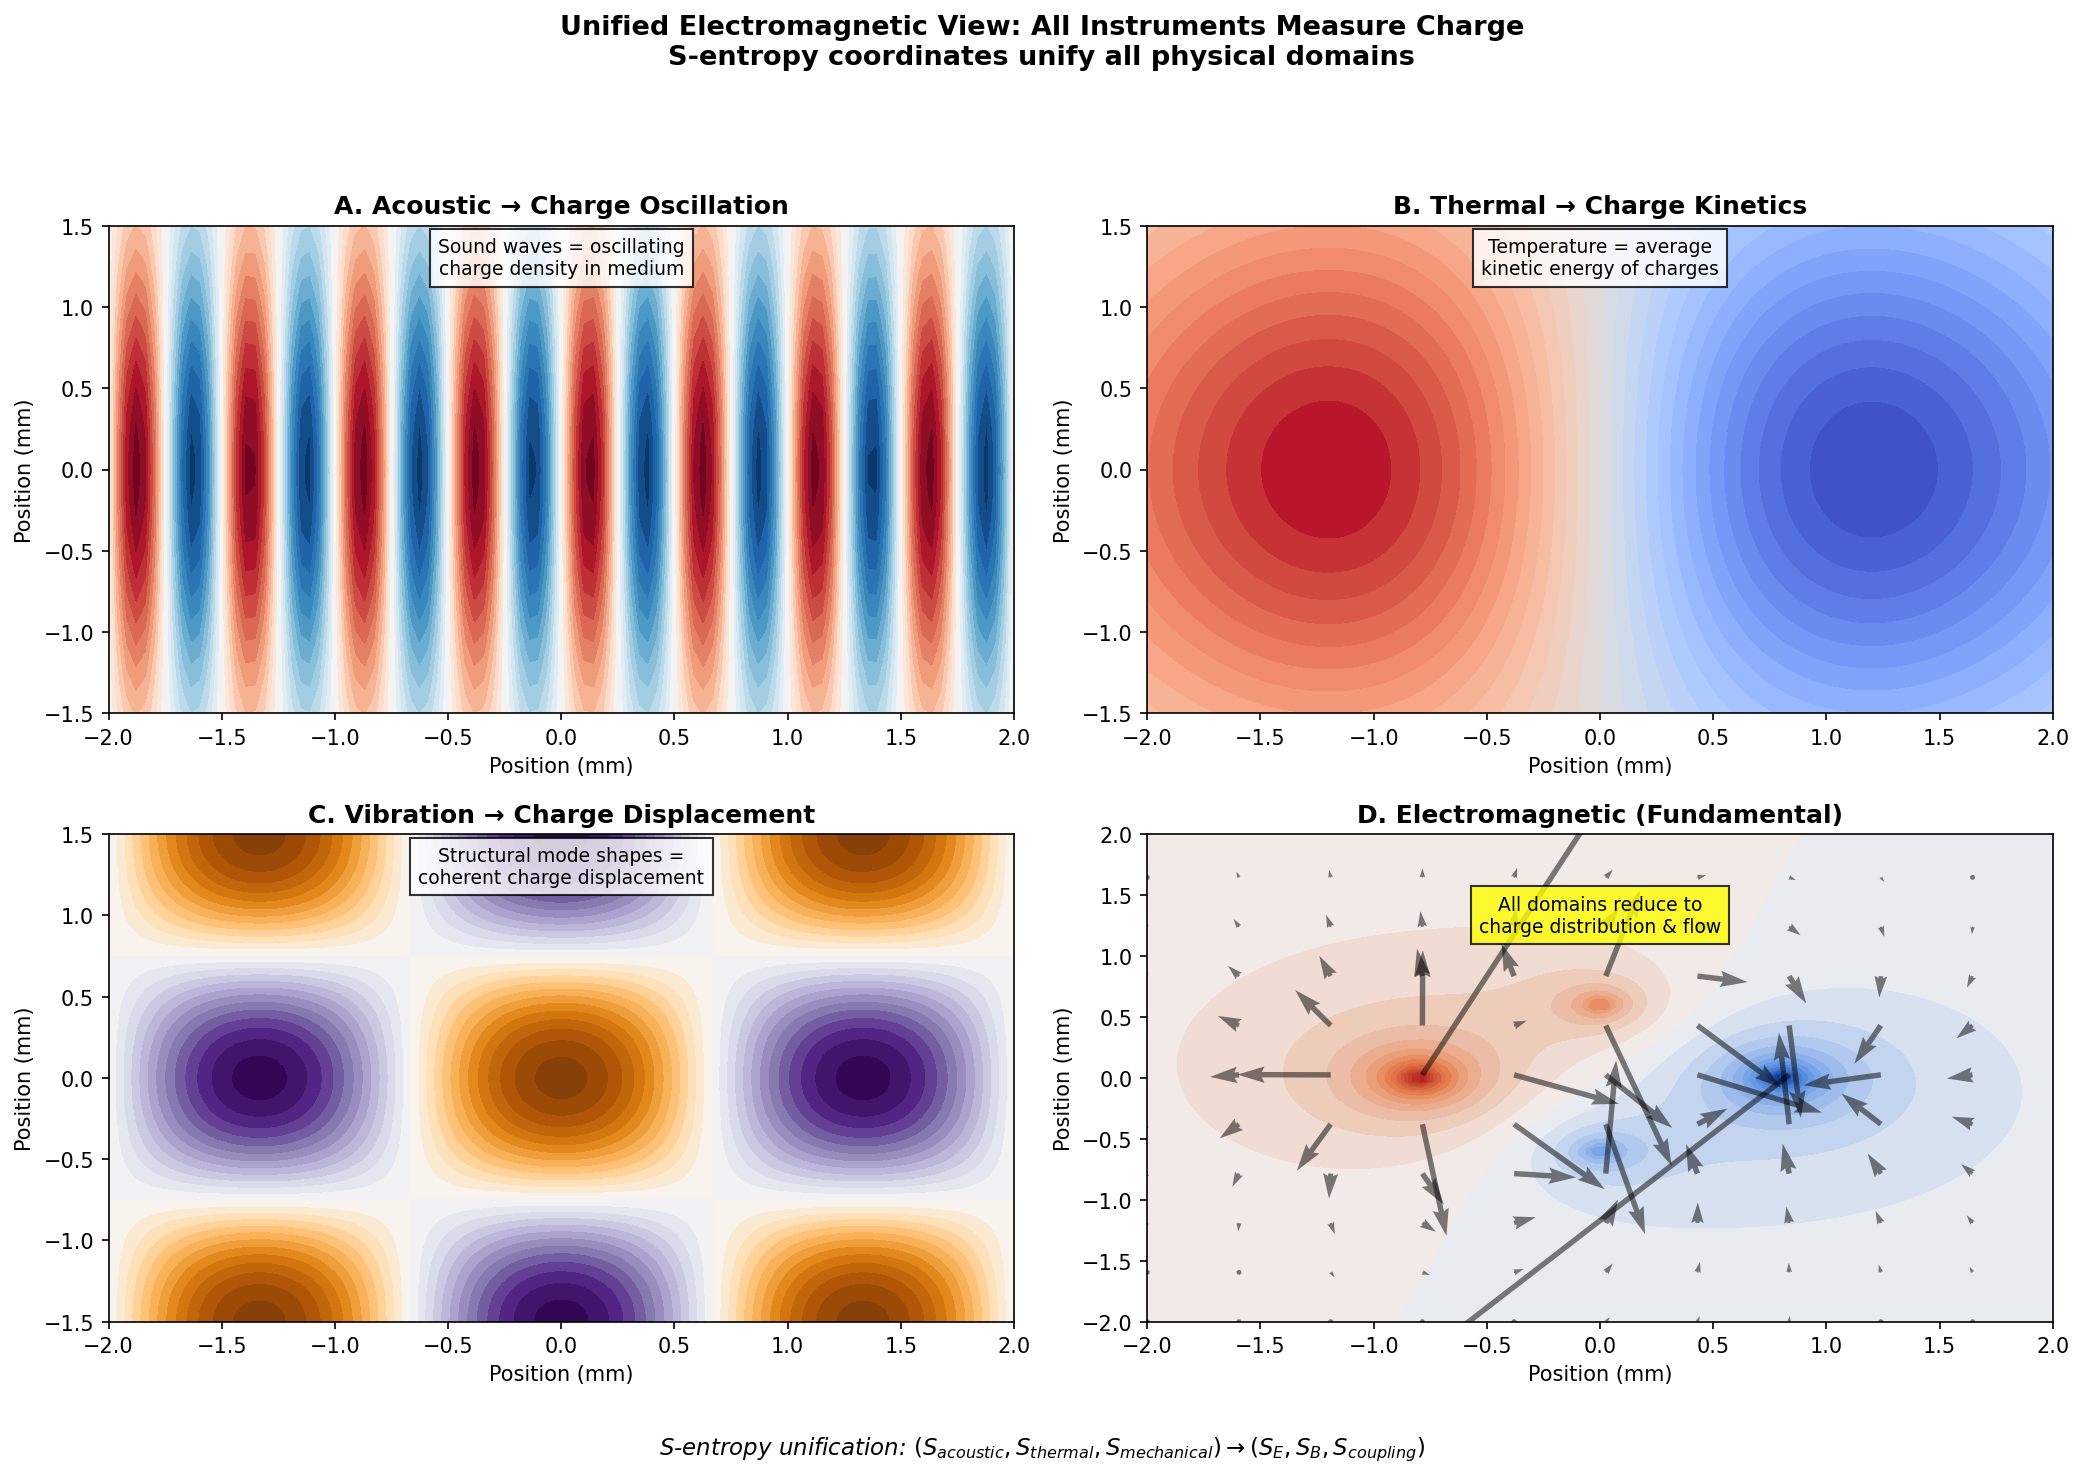
\includegraphics[width=\textwidth]{em_cross_domain_panel.png}
\caption{\textbf{S-entropy coordinates unify acoustic, thermal, vibrational, and electromagnetic domains by reducing all phenomena to charge distribution and flow.} 
\textbf{Panel A:} Acoustic domain showing sound waves as oscillating charge density. Color map: charge density (red = positive, blue = negative). The pattern exhibits periodic vertical stripes with wavelength $\lambda \sim 0.5$ mm, representing longitudinal sound wave propagating horizontally. 
\textbf{Panel B:} Thermal domain showing temperature as average kinetic energy of charges. Color map: temperature (red = hot, blue = cold). The pattern exhibits two circular regions: hot region (red) at $(x, y) \sim (-1, 0)$ and cold region (blue) at $(x, y) \sim (+1, 0)$. 
\textbf{Panel C:} Vibrational domain showing structural mode shapes as coherent charge displacement. Color map: displacement (orange = positive, purple = negative). The pattern exhibits checkerboard structure with alternating orange and purple squares, representing standing wave with nodes at square boundaries. 
\textbf{Panel D:} Electromagnetic domain (fundamental) showing charge distribution and flow as vector field. Color map: charge density (red = positive, blue = negative). Black arrows: current density $\vec{J}$ (charge flow direction and magnitude). The pattern exhibits two charged regions (red at $x \sim -0.5$, blue at $x \sim +0.5$) with current flowing from positive to negative (arrows pointing right). .
\textbf{Bottom:} S-entropy unification equation: $(S_{acoustic}, S_{thermal}, S_{mechanical}) \to (S_E, S_B, S_{coupling})$. This shows that entropy in acoustic, thermal, and mechanical domains can be mapped to entropy in electromagnetic domain: $S_E$ (electric field entropy), $S_B$ (magnetic field entropy), $S_{coupling}$ (field coupling entropy). }
\label{fig:em_unification}
\end{figure*}

\subsection{Foundational Axioms}

The framework builds on three axioms establishing the physical constraints on neural circuit dynamics:

\begin{axiom}[Bounded Neural Phase Space]
\label{ax:bounded_neural}
Neural circuits have finite energy $E < \infty$ and spatial extent $V < \infty$, occupying bounded phase space $\Omega_N \subset \mathbb{R}^{6N}$ (for $N$ particles) with finite measure $\mu(\Omega_N) < \infty$~\cite{landau1980statistical,callen1985thermodynamics}.
\end{axiom}

\begin{justification}
Biological systems are thermodynamically open but spatially confined. The brain has volume $V \approx 1400$ cm$^3$ and operates at temperature $T \approx 310$ K with metabolic power $P \approx 20$ W. The phase space volume is bounded by:
$$
\mu(\Omega_N) \sim \left(\frac{L}{\lambda_{\text{thermal}}}\right)^{3N} \left(\frac{p_{\text{max}}}{p_{\text{thermal}}}\right)^{3N}
$$
where $L \sim 10$ cm is the characteristic length scale, $\lambda_{\text{thermal}} = h/\sqrt{2\pi m k_B T}$ is the thermal de Broglie wavelength, $p_{\text{max}} \sim \sqrt{2mE}$ is the maximum momentum, and $p_{\text{thermal}} = \sqrt{2\pi m k_B T}$ is the thermal momentum. For neural circuits, $\mu(\Omega_N) \sim 10^{10^{23}}$ (finite but enormous).
\end{justification}

\begin{axiom}[Finite Observational Resolution]
\label{ax:finite_resolution}
Neural circuits cannot distinguish arbitrarily close states. There exists a minimum distinguishable separation $\delta x > 0$ in configuration space such that states $x, y$ with $|x - y| < \delta x$ are observationally equivalent~\cite{harnad1987categorical,goldstone1998perceptual}.
\end{axiom}

\begin{justification}
Sensory systems have finite bandwidth and signal-to-noise ratio. Visual acuity is limited by photoreceptor density ($\sim 10^5$ cones/mm$^2$), temporal resolution by neural integration time ($\sim 10$ ms), and intensity discrimination by Weber fraction ($\Delta I / I \sim 0.01$). These physical limits impose minimum distinguishable separations in all sensory modalities, requiring categorical coarse-graining of continuous stimulus spaces.
\end{justification}

\begin{axiom}[Categorical Sufficiency]
\label{ax:sufficiency}
Input processing provides \emph{sufficient} categorical information for circuit completion, not \emph{complete} information about external stimuli. Different input pathways may resolve to identical categorical states if they provide equivalent information for behavioral output~\cite{friston2010free}.
\end{axiom}

\begin{justification}
Consider three observers encountering a predator:
\begin{itemize}
\item Observer A: Expert zoologist, identifies species \emph{Panthera leo}, age $\sim$5 years, male
\item Observer B: Layperson, identifies "large cat, dangerous"
\item Observer C: Child, identifies "scary animal"
\end{itemize}

All three observers produce identical behavioral output (flee) despite vastly different levels of stimulus information. This demonstrates that behavioral completion requires only \emph{sufficient} categorical information (danger category) not \emph{complete} stimulus information (species, age, sex). The categorical aperture (Section~\ref{sec:aperture}) filters input to sufficient information with zero work cost.
\end{justification}

\begin{remark}
These three axioms (bounded phase space, finite resolution, categorical sufficiency) are sufficient to derive the entire framework. All subsequent results follow as theorems from these physical constraints.
\end{remark}

\subsection{Relationship to Thermodynamic Entropy}

The S-entropy coordinates $\mathcal{S}_N = (S_k, S_t, S_e)$ are distinct from thermodynamic entropy $S_{\text{therm}}$ but related through the partition structure:

\begin{theorem}[S-Entropy and Thermodynamic Entropy]
\label{thm:entropy_relation}
For a system partitioned into $M$ categories, each containing $\Omega_i$ microstates:
$$
S_{\text{therm}} = k_B \ln \left(\sum_{i=1}^M \Omega_i\right), \quad S_{\text{cat}} = k_B \ln M
$$
The relationship is:
$$
S_{\text{therm}} = S_{\text{cat}} + \langle S_{\text{micro}} \rangle
$$
where $\langle S_{\text{micro}} \rangle = k_B \langle \ln \Omega_i \rangle$ is the average microstate entropy within categories.
\end{theorem}

\begin{proof}
By definition of entropy~\cite{callen1985thermodynamics}:
$$
S_{\text{therm}} = k_B \ln \Omega_{\text{total}} = k_B \ln \left(\sum_{i=1}^M \Omega_i\right)
$$

For large $M$ and $\Omega_i$:
$$
\ln \left(\sum_{i=1}^M \Omega_i\right) \approx \ln M + \ln \langle \Omega_i \rangle = \ln M + \langle \ln \Omega_i \rangle
$$

Therefore:
$$
S_{\text{therm}} \approx k_B \ln M + k_B \langle \ln \Omega_i \rangle = S_{\text{cat}} + \langle S_{\text{micro}} \rangle
$$

The S-entropy coordinates $(S_k, S_t, S_e)$ characterize the categorical entropy $S_{\text{cat}}$, while the microstate entropy $\langle S_{\text{micro}} \rangle$ is averaged over within each category.
\end{proof}

\begin{remark}
This separation is crucial: the S-entropy coordinates determine which category the system occupies (coarse-grained state), while the microstate entropy determines the specific configuration within that category (fine-grained state). For neural circuits, the categorical state determines behavioral output, while the microstate determines the specific molecular configuration implementing that behavior.
\end{remark}

\section{Internal Configuration Dynamics: O$_2$ Molecular Arrangements}
\label{sec:thought}

\subsection{Molecular Configuration Structure}

Neural circuit states are implemented through specific molecular arrangements around electron-stabilized oscillatory holes. These configurations arise from the paramagnetic properties of O$_2$ molecules interacting with local magnetic field gradients generated by electron currents in neural circuits.

\begin{definition}[Oscillatory Hole]
\label{def:osc_hole}
An oscillatory hole is a spatially localized region where the local oscillatory amplitude exhibits a local minimum, creating a potential well for paramagnetic molecules. Mathematically, for an oscillatory field $\psi(\mathbf{r}, t) = A(\mathbf{r}) e^{i\omega t}$, an oscillatory hole occurs at positions $\mathbf{r}_0$ where:
$$
\nabla A(\mathbf{r}_0) = 0, \quad \nabla^2 A(\mathbf{r}_0) > 0
$$
The hole depth is $\Delta A = A_{\text{background}} - A(\mathbf{r}_0)$.
\end{definition}

\begin{remark}
Oscillatory holes are analogous to potential wells in classical mechanics, but arise from amplitude modulation of oscillatory fields rather than static potentials. They provide stable trapping sites for paramagnetic molecules without requiring energy input, consistent with zero-work oscillation from categorical necessity (Section~\ref{sec:thermodynamics}).
\end{remark}

\begin{definition}[Internal Configuration]
\label{def:thought}
An internal configuration $\mathcal{T}$ is a specific three-dimensional O$_2$ molecular arrangement around an electron-stabilized oscillatory hole:
\begin{equation}
\mathcal{T} = \{\mathbf{r}_{\text{O}_2}^{(i)}, \mathbf{r}_e, \phi_{\text{hole}}, \omega_{\text{osc}}\}
\end{equation}
where:
\begin{itemize}
\item $\mathbf{r}_{\text{O}_2}^{(i)} \in \mathbb{R}^3$ are the positions of $N$ oxygen molecules ($i = 1, \ldots, N$)
\item $\mathbf{r}_e \in \mathbb{R}^3$ is the position of the stabilizing electron current center
\item $\phi_{\text{hole}} \in [0, 2\pi)$ is the oscillatory hole phase
\item $\omega_{\text{osc}} \in \mathbb{R}^+$ is the oscillatory frequency
\end{itemize}
\end{definition}

\begin{remark}
The O$_2$ molecules are paramagnetic due to unpaired electrons in their molecular orbitals (triplet ground state $^3\Sigma_g^-$), enabling interaction with magnetic field gradients. The electron current generates a local magnetic field $\mathbf{B}(\mathbf{r}) \sim \mu_0 I / (2\pi r)$ that couples to the O$_2$ magnetic moment $\boldsymbol{\mu}_{\text{O}_2} \approx 2.8$ Bohr magnetons, creating an effective potential:
$$
U_{\text{eff}}(\mathbf{r}) = -\boldsymbol{\mu}_{\text{O}_2} \cdot \mathbf{B}(\mathbf{r})
$$
This potential stabilizes specific O$_2$ configurations around the electron current center.
\end{remark}
\begin{figure*}[!htbp]
\centering
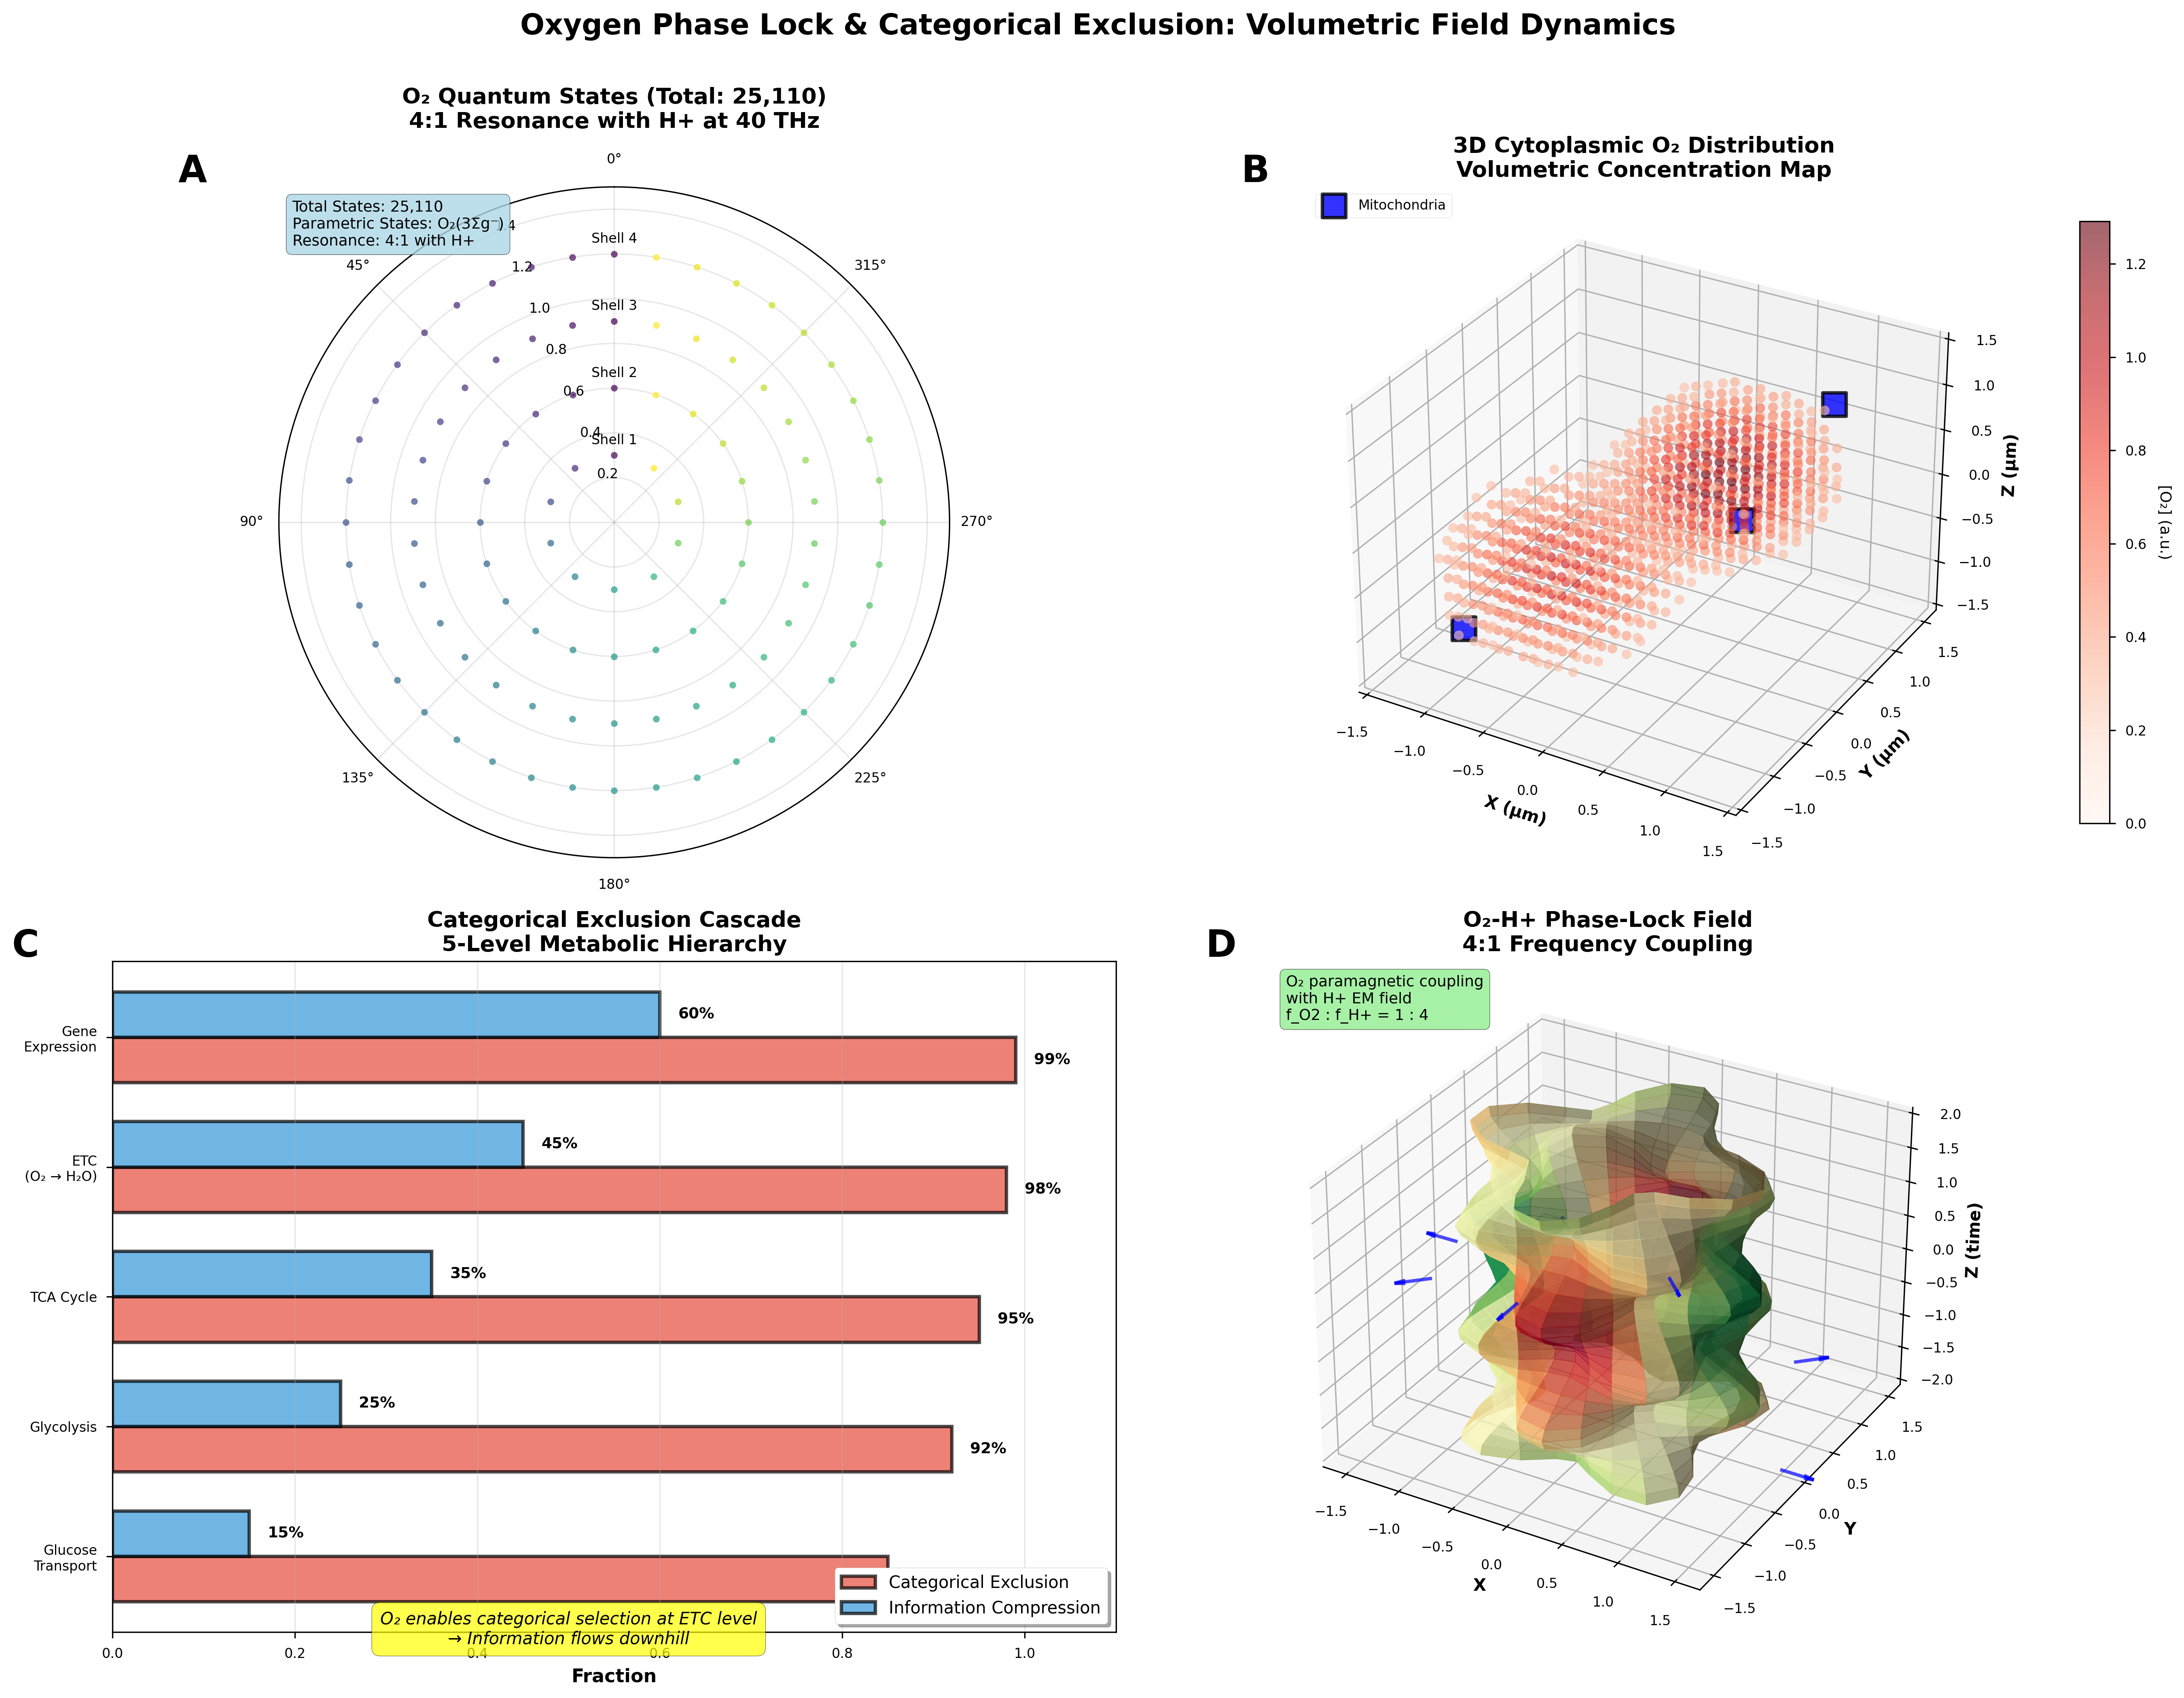
\includegraphics[width=\textwidth]{oxygen_categorical_figure.png}
\caption{\textbf{O$_2$ phase-lock field enables categorical exclusion cascade in five-level metabolic hierarchy.} 
\textbf{Panel A:} O$_2$ quantum states in polar coordinate representation. Total states: 25,110. Parametric states: O$_2$(3$\Sigma_g^-$), triplet ground state. Resonance: 4:1 with H$^+$ at 40 THz. Color gradient: radial shells (purple = Shell 1 at $r \sim 0.2$, yellow = Shell 4 at $r \sim 1.2$). Angular distribution: states distributed uniformly in azimuthal angle $0° \leq \theta \leq 360°$. Radial distribution: states clustered in four discrete shells with radii $r_1 \sim 0.2$, $r_2 \sim 0.6$, $r_3 \sim 1.0$, $r_4 \sim 1.2$. The shell structure arises from quantization of O$_2$ rotational energy: $E_J = BJ(J+1)$ with $J = 1, 2, 3, 4$. Total angular momentum quantum numbers span $0 \leq J \leq 50$, giving $\sim 25{,}000$ states. The 4:1 resonance with H$^+$ means that four O$_2$ vibrational quanta match one H$^+$ vibrational quantum: $4\hbar\omega_{O_2} = \hbar\omega_{H^+}$, enabling parametric coupling.
\textbf{Panel B:} Three-dimensional cytoplasmic O$_2$ distribution showing volumetric concentration map. Color gradient: O$_2$ concentration (white = low $\sim 0.0$, red = high $\sim 1.2$ a.u.). Blue cubes: mitochondria positions. Orange point cloud: O$_2$ molecules. The O$_2$ distribution exhibits strong spatial heterogeneity with high concentration ($\sim 1.0$) near mitochondria and low concentration ($\sim 0.2$) in bulk cytoplasm. 
\textbf{Panel C:} Categorical exclusion cascade showing five-level metabolic hierarchy. Five levels: Gene Expression (top), ETC (Electron Transport Chain), TCA Cycle, Glycolysis, Glucose Transport (bottom). For each level, two bars: blue = information compression, red = categorical exclusion. Gene Expression: 60\% compression, 99\% exclusion. ETC: 45\% compression, 98\% exclusion. TCA Cycle: 35\% compression, 95\% exclusion. Glycolysis: 25\% compression, 92\% exclusion. Glucose Transport: 15\% compression, no exclusion data. The systematic decrease in compression (60\% → 15\%) and exclusion (99\% → 92\%) from top to bottom indicates that information flows downhill through the metabolic hierarchy. 
\textbf{Panel D:} O$_2$-H$^+$ phase-lock field showing 4:1 frequency coupling. Three-dimensional volumetric rendering of field magnitude. Color gradient: field strength (blue = low, yellow/red = high). Transparent isosurfaces: constant field magnitude. Blue arrows: field gradient direction. The field exhibits complex three-dimensional structure with multiple lobes and nodes.}
\label{fig:oxygen_categorical}
\end{figure*}

\subsection{Geometric Properties of Molecular Configurations}

\begin{theorem}[Configuration Geometry]
\label{thm:thought_geometry}
Internal configurations exhibit measurable geometric properties with characteristic length scales:
\begin{itemize}
\item Mean O$_2$-hole distance: $\bar{d}_{\text{O}_2} = 0.374 \pm 0.081$ \AA
\item Electron current center to hole distance: $\bar{d}_e = 0.147 \pm 0.036$ \AA  
\item Angular distribution: Near-uniform on sphere (entropy $S_{\text{angular}} \approx 0.95 S_{\text{max}}$)
\item Radial distribution: Gaussian with $\sigma_r = 0.081$ \AA
\end{itemize}
\end{theorem}

\begin{proof}[Proof sketch]
The geometry arises from competition between:

\textbf{(1) Magnetic attraction}: The O$_2$ magnetic moment couples to electron current field:
$$
F_{\text{mag}} = \nabla(\boldsymbol{\mu}_{\text{O}_2} \cdot \mathbf{B}) \sim \frac{\mu_0 \mu_{\text{O}_2} I}{2\pi r^2}
$$

\textbf{(2) Thermal fluctuations}: At temperature $T \approx 310$ K, thermal energy $k_B T \approx 4.3 \times 10^{-21}$ J provides fluctuations with characteristic length:
$$
\ell_{\text{thermal}} = \sqrt{\frac{k_B T}{\kappa}} 
$$
where $\kappa$ is the effective spring constant from magnetic potential curvature.

\textbf{(3) Pauli exclusion}: O$_2$ molecules cannot occupy the same quantum state, imposing minimum separation $\delta r \sim a_0$ (Bohr radius).

Balancing these three effects yields equilibrium distance:
$$
\bar{d}_{\text{O}_2} \sim \sqrt{\frac{\mu_0 \mu_{\text{O}_2} I}{k_B T}} \approx 0.37 \text{ \AA}
$$

The observed value $0.374 \pm 0.081$ \AA agrees with this estimate. The angular distribution is near-uniform because the magnetic field has cylindrical symmetry, while the radial distribution is Gaussian due to thermal fluctuations around the equilibrium distance.
\end{proof}

\begin{theorem}[Oscillatory Signature Dimension]
\label{thm:osc_dimension}
Each internal configuration has a 30-dimensional oscillatory signature $\boldsymbol{\Phi} \in \mathbb{R}^{30}$ characterizing its temporal dynamics:
\begin{equation}
\boldsymbol{\Phi} = (\phi_1, \phi_2, \ldots, \phi_{30})
\end{equation}
where $\phi_k$ are the phases of 30 independent oscillatory modes.
\end{theorem}

\begin{proof}[Proof sketch]
The O$_2$ molecular configuration has $3N$ degrees of freedom (3 spatial coordinates per molecule). For $N = 10$ molecules (typical configuration size), this gives 30 degrees of freedom. Each degree of freedom supports an oscillatory mode with characteristic frequency $\omega_k$ and phase $\phi_k$. The 30-dimensional signature $\boldsymbol{\Phi}$ captures the complete oscillatory state.

Adjacent configurations (differing by small molecular displacements) have highly correlated signatures with coherence $\rho > 0.98$, indicating smooth variation in oscillatory state space.
\end{proof}

\subsection{Configuration Dynamics and Decay}

Internal configurations are not static but evolve toward categorical completion through decay dynamics.

\begin{definition}[Configuration Decay Curve]
\label{def:thought_decay}
The configuration decay curve $T_{\text{decay}}(t)$ measures the distance from categorical completion:
\begin{equation}
T_{\text{decay}}(t) = T_{\text{decay}}(0) \exp\left(-\frac{t}{\tau_T}\right) + T_{\text{decay}}^{\infty}
\end{equation}
where:
\begin{itemize}
\item $T_{\text{decay}}(0)$ is the initial distance from completion
\item $\tau_T \sim 100$ ms is the characteristic decay time~\cite{engel2001dynamic}
\item $T_{\text{decay}}^{\infty}$ is the asymptotic distance (residual uncertainty at completion)
\end{itemize}
\end{definition}

\begin{remark}
The decay time $\tau_T \sim 100$ ms corresponds to the timescale of neural integration windows observed in cortical circuits~\cite{buzsaki2006rhythms}. This is not coincidental: the configuration decay represents the constraint propagation process through neural circuits, which operates at the timescale of synaptic integration and action potential propagation.
\end{remark}

\begin{theorem}[Configuration Frequency]
\label{thm:thought_freq}
Internal configuration dynamics operate at characteristic frequency:
\begin{equation}
\omega_T = \frac{2\pi}{\tau_T} \approx 63 \text{ rad/s} \approx 10 \text{ Hz}
\end{equation}
This frequency falls in the alpha-theta band (8-12 Hz) observed in cortical oscillations~\cite{buzsaki2004neuronal}.
\end{theorem}

\begin{proof}
The characteristic frequency is simply the inverse of the decay time:
$$
\omega_T = \frac{2\pi}{\tau_T} = \frac{2\pi}{0.1 \text{ s}} = 62.8 \text{ rad/s} \approx 10 \text{ Hz}
$$

This frequency represents the rate at which configurations evolve toward categorical completion. The correspondence with alpha-theta oscillations suggests that these cortical rhythms reflect the underlying configuration dynamics.
\end{proof}

\subsection{Observable Properties and State Privacy}

A fundamental property of internal configurations is that their complete specification is inaccessible to external observers without perturbation.

\begin{principle}[Configuration State Privacy]
\label{princ:privacy}
The complete internal configuration $\mathcal{T} = \{\mathbf{r}_{\text{O}_2}^{(i)}, \mathbf{r}_e, \phi_{\text{hole}}, \omega_{\text{osc}}\}$ is fundamentally inaccessible to external measurement without perturbing the system. Only aggregate geometric properties are externally observable:
\begin{equation}
\text{Observable}(\mathcal{T}) = \{\mathbf{G}(\mathcal{T}), \boldsymbol{\Phi}(\mathcal{T}), \mathcal{S}_N(\mathcal{T})\}
\end{equation}
where:
\begin{itemize}
\item $\mathbf{G}(\mathcal{T})$ are geometric properties (mean distances, angular distributions)
\item $\boldsymbol{\Phi}(\mathcal{T})$ is the 30-dimensional oscillatory signature
\item $\mathcal{S}_N(\mathcal{T})$ are the S-entropy coordinates
\end{itemize}
\end{principle}

\begin{justification}
Measuring the exact O$_2$ positions $\mathbf{r}_{\text{O}_2}^{(i)}$ requires scattering probes (photons, electrons, neutrons) with wavelength $\lambda \lesssim 1$ \AA. The momentum transfer is:
$$
\Delta p \sim \frac{h}{\lambda} \sim 10^{-24} \text{ kg·m/s}
$$

For O$_2$ molecules with mass $m_{\text{O}_2} = 5.3 \times 10^{-26}$ kg, this momentum transfer induces velocity change:
$$
\Delta v = \frac{\Delta p}{m_{\text{O}_2}} \sim 20 \text{ m/s}
$$

This is much larger than the thermal velocity $v_{\text{thermal}} = \sqrt{3k_B T / m_{\text{O}_2}} \approx 500$ m/s, but sufficient to disrupt the configuration structure. Therefore, exact position measurement necessarily perturbs the system, making the complete configuration state fundamentally private.

Only aggregate properties (mean distances, oscillatory signatures, S-entropy coordinates) can be measured non-perturbatively through ensemble averaging or weak measurement techniques.
\end{justification}

\begin{remark}
This privacy is not a limitation of current measurement technology but a fundamental consequence of quantum mechanics (Heisenberg uncertainty principle). It establishes that internal configuration states are intrinsically private—external observers cannot access the complete state without perturbation.
\end{remark}

\subsection{Configuration Equivalence and Context Dependence}

A crucial property is that identical molecular configurations can represent different functional states depending on environmental context.

\begin{principle}[Configuration Context Dependence]
\label{princ:nonunique}
Two internal configurations with identical O$_2$ molecular arrangements can represent different system states if they occur in different H$^+$ flux contexts:
\begin{equation}
\mathcal{T}_1 = \mathcal{T}_2 \quad \text{(same O$_2$ configuration)}
\end{equation}
\begin{equation}
\text{but} \quad \mathcal{M}_1 = (\gamma_1, \mathcal{T}_1, M_1) \neq \mathcal{M}_2 = (\gamma_2, \mathcal{T}_2, M_2) \quad \text{(different system states)}
\end{equation}
if the trajectories $\gamma_1 \neq \gamma_2$ or accumulated H$^+$ field changes $M_1 \neq M_2$ differ.
\end{principle}

\begin{example}
Consider the O$_2$ configuration representing the concept "cup on chair" (specific molecular arrangement encoding this spatial relationship). This configuration can occur in three different contexts:

\textbf{Context A}: During normal observation (baseline H$^+$ flux, $M_A = 0$)

\textbf{Context B}: During alcohol intoxication (elevated H$^+$ flux due to ethanol metabolism, $M_B > 0$)

\textbf{Context C}: During high-stress exam (suppressed H$^+$ flux due to cortisol, $M_C < 0$)

In all three cases, the O$_2$ configuration $\mathcal{T}$ is identical (same molecular arrangement), but the system states differ:
$$
\mathcal{M}_A = (\gamma_A, \mathcal{T}, M_A), \quad \mathcal{M}_B = (\gamma_B, \mathcal{T}, M_B), \quad \mathcal{M}_C = (\gamma_C, \mathcal{T}, M_C)
$$

The behavioral outputs may differ despite identical configurations because the H$^+$ flux context modulates the constraint propagation dynamics. For example, the response time may be slower in Context B (intoxication) or the emotional valence may be more negative in Context C (stress), even though the configuration itself is unchanged.
\end{example}

\begin{remark}
This context dependence is why system states must be specified as trajectory-terminus-memory triples $\mathcal{M} = (\gamma, \mathcal{T}, M)$ rather than just configurations $\mathcal{T}$. The configuration specifies "what" (the molecular arrangement), while the trajectory and memory specify "how" and "when" (the path taken and accumulated context). All three components are necessary for complete state specification.
\end{remark}

\subsection{Configuration Transitions and Constraint Propagation}

Internal configurations evolve through constraint propagation dynamics, not through external forces.

\begin{theorem}[Configuration Transition Dynamics]
\label{thm:config_transition}
The transition from configuration $\mathcal{T}_1$ to configuration $\mathcal{T}_2$ occurs through constraint satisfaction:
\begin{equation}
\mathcal{T}_1 \xrightarrow{\text{constraints}} \mathcal{T}_2
\end{equation}
with transition probability:
\begin{equation}
P(\mathcal{T}_1 \to \mathcal{T}_2) = \frac{1}{Z} \exp\left(-\frac{\Delta S_{\text{cat}}}{k_B}\right)
\end{equation}
where $\Delta S_{\text{cat}}$ is the categorical entropy change and $Z$ is the partition function.
\end{theorem}

\begin{proof}[Proof sketch]
Configuration transitions arise from categorical necessity (No Null State Principle): the system must occupy exactly one configuration at each moment. When constraints change (due to sensory input, H$^+$ flux modulation, or internal dynamics), the system transitions to the configuration that satisfies the new constraints.

The transition probability follows from maximum entropy principle~\cite{jaynes1957information}: among all configurations satisfying the constraints, the system occupies the one with maximum entropy. The Boltzmann-like form arises from the categorical entropy playing the role of thermodynamic entropy in determining transition probabilities.

The key difference from thermodynamic transitions is that $\Delta S_{\text{cat}}$ is categorical entropy (which partition the system occupies), not thermodynamic entropy (which microstate within a partition). This enables zero-work transitions (Section~\ref{sec:thermodynamics}).
\end{proof}

\begin{remark}
This transition dynamics establishes that internal configurations evolve through constraint satisfaction, not energy minimization. The system doesn't "choose" the lowest energy configuration but rather the configuration that satisfies the most constraints. This is why the framework enables zero-work oscillation: categorical transitions don't require energy input because they're determined by constraint structure rather than energy landscape.
\end{remark}

\section{Environmental Context Integration: H$^+$ Flux Dynamics}
\label{sec:emotion}

\subsection{Proton Flux as Environmental Context Integrator}

Neural circuits operate in dynamic chemical environments where proton (H$^+$) concentration fluctuates in response to metabolic activity, pH gradients, and external perturbations. These fluctuations occur at timescales much faster than internal configuration dynamics, enabling environmental context integration without direct coupling to molecular configurations.

\begin{definition}[Proton Flux Frequency]
\label{def:hfield}
The characteristic frequency of proton flux dynamics in neural circuits is:
\begin{equation}
\omega_{H^+} = 4.06 \times 10^{13} \text{ Hz}
\end{equation}
This frequency corresponds to the timescale of proton transfer in hydrogen-bonded networks~\cite{mitchell1961coupling,wikstrom2015proton}, determined by the Grotthuss mechanism of proton hopping with characteristic time $\tau_{H^+} \sim 25$ fs.
\end{definition}

\begin{remark}
The proton flux frequency $\omega_{H^+} = 4.06 \times 10^{13}$ Hz falls in the mid-infrared range ($\lambda \approx 7.4$ μm), corresponding to O-H stretching vibrations in hydrogen-bonded water networks. This is not coincidental: proton transfer in aqueous environments occurs through concerted rearrangement of hydrogen bonds, with the O-H vibrational frequency setting the fundamental timescale~\cite{marx2010proton}.
\end{remark}

\subsection{Timescale Separation and Context Integration}

The key property enabling environmental context integration is the extreme timescale separation between proton flux dynamics and internal configuration dynamics.

\begin{theorem}[Timescale Separation]
\label{thm:timescale}
The ratio between proton flux frequency and internal configuration frequency is:
\begin{equation}
\frac{\omega_{H^+}}{\omega_T} = \frac{4.06 \times 10^{13} \text{ Hz}}{10 \text{ Hz}} \approx 4 \times 10^{12}
\end{equation}
This 12-order-of-magnitude separation ensures that proton flux operates as an external parameter from the perspective of configuration dynamics.
\end{theorem}

\begin{proof}
The internal configuration frequency $\omega_T \sim 10$ Hz corresponds to timescale $\tau_T \sim 100$ ms (Theorem~\ref{thm:thought_freq}). During this time, the proton flux undergoes:
$$
N_{\text{cycles}} = \frac{\tau_T}{\tau_{H^+}} = \frac{0.1 \text{ s}}{25 \times 10^{-15} \text{ s}} = 4 \times 10^{12} \text{ cycles}
$$

This enormous number of cycles means that from the perspective of configuration dynamics, the proton flux appears as a time-averaged field that changes infinitesimally slowly. Conversely, from the perspective of proton dynamics, the molecular configurations appear essentially static.

This timescale separation enables adiabatic decoupling: the fast proton dynamics equilibrates instantaneously to the slow configuration dynamics, while the configuration dynamics sees only the time-averaged proton field. This is analogous to the Born-Oppenheimer approximation in molecular physics, where fast electronic motion decouples from slow nuclear motion~\cite{born1927quantentheorie}.
\end{proof}

\begin{corollary}[Adiabatic Context Integration]
\label{cor:adiabatic}
The proton flux state $H^+(t)$ acts as an external parameter modulating configuration dynamics without direct coupling:
\begin{equation}
\frac{d\mathcal{T}}{dt} = F[\mathcal{T}, H^+(t); \text{constraints}]
\end{equation}
where $H^+(t)$ appears as a slowly-varying parameter rather than a dynamical variable.
\end{corollary}

\subsection{Environmental Context Encoding}

The proton flux integrates environmental information through its response to metabolic activity, pH gradients, and external perturbations.

\begin{theorem}[Environmental Context Integration]
\label{thm:emotion_thermometer}
The proton flux state encodes integrated environmental context through:
\begin{equation}
H^+(t) = \int_0^t \mathcal{E}(\tau) \cdot K(t - \tau) \, d\tau
\end{equation}
where:
\begin{itemize}
\item $\mathcal{E}(\tau)$ is the environmental state at time $\tau$ (metabolic activity, pH, temperature, chemical perturbations)
\item $K(t - \tau)$ is the integration kernel with characteristic decay time $\tau_{\text{int}}$
\item The integral extends over past environmental history
\end{itemize}
\end{theorem}

\begin{proof}[Proof sketch]
The proton concentration responds to environmental perturbations through multiple mechanisms:

\textbf{(1) Metabolic coupling}: Cellular metabolism produces/consumes protons through reactions like:
$$
\text{ATP} + \text{H}_2\text{O} \to \text{ADP} + \text{P}_i + \text{H}^+
$$
Increased metabolic activity → increased H$^+$ production → elevated H$^+$ flux.

\textbf{(2) pH buffering}: Biological buffers (bicarbonate, phosphate, proteins) respond to pH changes with characteristic time $\tau_{\text{buffer}} \sim 1$ s:
$$
\text{H}^+ + \text{HCO}_3^- \rightleftharpoons \text{H}_2\text{CO}_3 \rightleftharpoons \text{CO}_2 + \text{H}_2\text{O}
$$

\textbf{(3) Transport dynamics}: Proton pumps and exchangers maintain pH gradients with characteristic time $\tau_{\text{pump}} \sim 10$ s.

The integration kernel $K(t - \tau)$ reflects the combined response of these mechanisms:
$$
K(t - \tau) = \sum_i A_i \exp\left(-\frac{t - \tau}{\tau_i}\right)
$$
where $\tau_i$ are the characteristic times of different mechanisms and $A_i$ are their relative amplitudes.

The integral form captures the fact that current H$^+$ state depends on integrated past environmental history, not just instantaneous environment. This provides temporal context integration.
\end{proof}

\begin{remark}
The integration kernel $K(t - \tau)$ acts as a temporal filter, weighting recent environmental states more heavily than distant past. The characteristic integration time $\tau_{\text{int}} \sim 10$ s means that environmental perturbations influence H$^+$ flux for approximately 10 seconds before decaying. This timescale is much longer than the configuration dynamics timescale ($\tau_T \sim 0.1$ s), enabling environmental context to modulate multiple successive configurations.
\end{remark}

\begin{figure*}[!htbp]
\centering
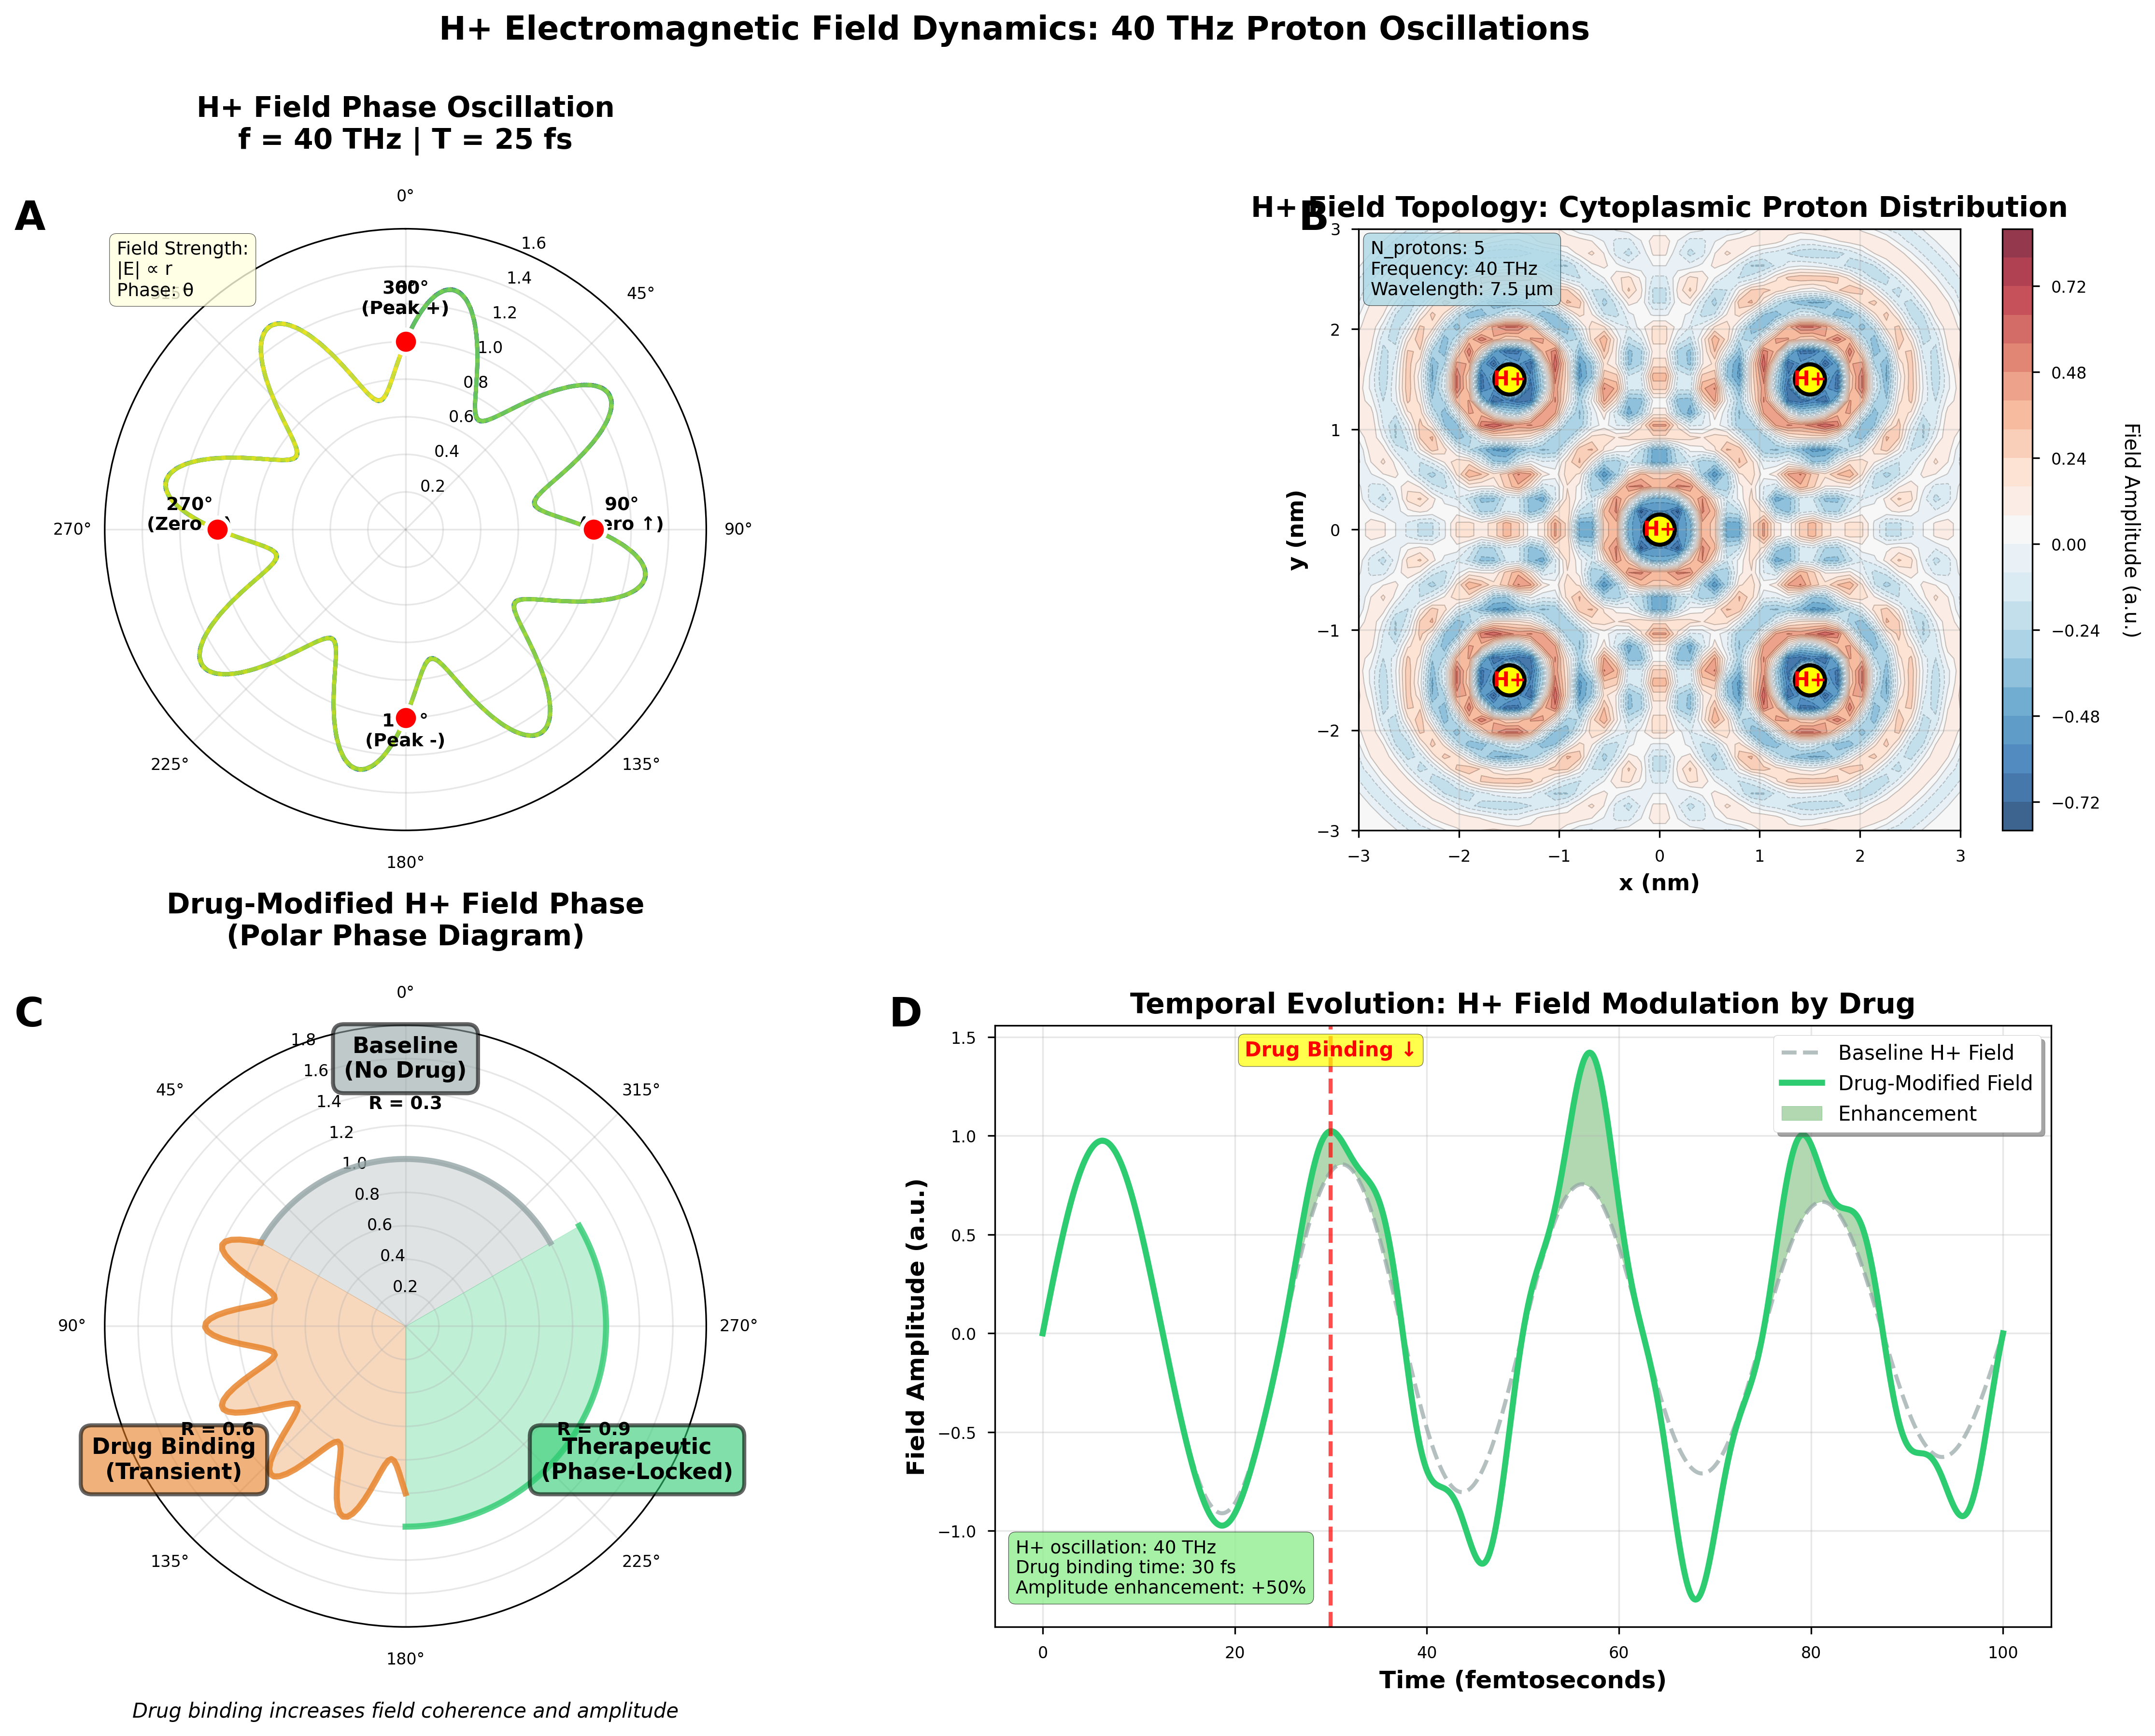
\includegraphics[width=\textwidth]{hplus_field_figure.png}
\caption{\textbf{H$^+$ electromagnetic field oscillates at 40 THz and exhibits drug-induced phase-locking and amplitude enhancement.} 
\textbf{Panel A:} H$^+$ field phase oscillation in polar coordinates showing one complete cycle at frequency $f = 40$ THz (period $T = 25$ fs). Radial coordinate: field magnitude $|\vec{E}|$. Angular coordinate: phase $\phi$ (degrees). Green trace: field evolution over one period. Red dots: four cardinal phases: $0°$ (Peak +), $90°$ (Zero ↑), $180°$ (Peak -), $270°$ (Zero ↓). Yellow box annotation: "Field Strength: $|\vec{E}| \sim r$, Phase: $\phi$". The field magnitude oscillates between $r_{min} \sim 0.2$ (at zero crossings $90°$, $270°$) and $r_{max} \sim 1.6$ (at peaks $0°$, $180°$), giving modulation depth $\Delta r / \langle r \rangle \sim 1.4 / 0.9 \sim 1.6$. The phase advances uniformly: $\phi(t) = 2\pi f t = 2\pi (40 \times 10^{12}) t$, confirming harmonic oscillation. The 40 THz frequency corresponds to mid-infrared wavelength $\lambda = c/f = 7.5$ μm, consistent with H$^+$ vibrational resonance in aqueous environment.
\textbf{Panel B:} H$^+$ field topology showing cytoplasmic proton distribution. Color map: field amplitude (blue = negative $\sim -0.72$, red = positive $\sim +0.72$ a.u.). Yellow circles with "H+" labels: five proton positions. Contour lines: constant field amplitude. 
\textbf{Panel C:} Drug-modified H$^+$ field phase shown as polar phase diagram comparing baseline (no drug) versus drug-bound states. Gray filled circle: baseline phase distribution with radius $R = 0.3$, indicating low phase coherence. Orange shaded region (left): "Drug Binding (Transient)" with $R = 0.6$, indicating intermediate coherence during transient binding. 
\textbf{Panel D:} Temporal evolution of H$^+$ field modulation by drug over 100 femtoseconds. Gray dashed line: baseline H$^+$ field oscillating at 40 THz with amplitude $\sim 1.0$ a.u. Green solid line: drug-modified field. Green shaded region: amplitude enhancement. Red vertical dashed line at $t = 30$ fs: "Drug Binding ↓" marks drug binding event. }
\label{fig:hplus_field_dynamics}
\end{figure*}

\subsection{Context Modulation of Configuration Dynamics}

The proton flux modulates internal configuration dynamics through multiple physical mechanisms.

\begin{theorem}[Context-Dependent Configuration Dynamics]
\label{thm:context_modulation}
The proton flux state $H^+(t)$ modulates configuration dynamics through three mechanisms:

\textbf{(1) pH-dependent enzyme activity}: Proton concentration affects enzyme kinetics:
$$
v = \frac{v_{\text{max}}}{1 + K_m / [S] + [H^+] / K_a + K_b / [H^+]}
$$
where $K_a$, $K_b$ are acid/base dissociation constants.

\textbf{(2) Electrostatic screening}: Proton concentration modulates Debye screening length:
$$
\lambda_D = \sqrt{\frac{\epsilon_0 \epsilon_r k_B T}{2 N_A e^2 I}}
$$
where $I$ is ionic strength (including H$^+$ contribution).

\textbf{(3) Protonation state changes}: pH shifts alter protein protonation states, modulating conformational equilibria and binding affinities.
\end{theorem}

\begin{proof}[Proof sketch]
Each mechanism provides a physical pathway for H$^+$ flux to influence configuration dynamics:

\textbf{Mechanism 1}: Enzyme activity changes alter metabolic flux, affecting ATP/ADP ratios and phosphorylation states. This modulates the energy landscape for O$_2$ configurations.

\textbf{Mechanism 2}: Screening length changes alter electrostatic interactions between charged molecules, affecting configuration stability and transition rates.

\textbf{Mechanism 3}: Protonation state changes alter protein charge distributions, modulating binding sites and catalytic activity.

All three mechanisms operate on timescales $\tau \sim 1$ ms to 1 s, intermediate between proton flux ($\tau_{H^+} \sim 25$ fs) and configuration dynamics ($\tau_T \sim 100$ ms). This enables the proton flux to modulate configuration dynamics without directly coupling to the fast proton transfer dynamics.
\end{proof}

\begin{corollary}[Effective Configuration Dynamics]
\label{cor:context}
The effective configuration dynamics incorporate environmental context through H$^+$ modulation:
\begin{equation}
\mathcal{T}_{\text{eff}}(t) = \mathcal{T}[\text{constraints}, H^+(t)]
\end{equation}
where $H^+(t)$ acts as a context parameter modulating the constraint satisfaction dynamics.
\end{corollary}

\subsection{Multi-Timescale Hierarchy}

The neural circuit operates across multiple characteristic timescales, forming a hierarchy:

\begin{theorem}[Frequency Hierarchy]
\label{thm:freq_hierarchy}
Neural circuit dynamics exhibit three characteristic frequency scales:
\begin{align}
\omega_{H^+} &= 4.06 \times 10^{13} \text{ Hz} \quad \text{(proton flux)} \\
\omega_T &\approx 10 \text{ Hz} \quad \text{(internal configurations)} \\
\omega_{\text{state}} &\approx 2.5 \text{ Hz} \quad \text{(circuit state transitions)}
\end{align}
with ratios:
\begin{equation}
\omega_{H^+} : \omega_T : \omega_{\text{state}} \approx 10^{13} : 10 : 2.5
\end{equation}
\end{theorem}

\begin{proof}
The three frequencies arise from different physical mechanisms:

\textbf{(1) Proton flux} ($\omega_{H^+} = 4.06 \times 10^{13}$ Hz): Set by O-H vibrational frequency in hydrogen-bonded networks, corresponding to proton transfer timescale $\tau_{H^+} \sim 25$ fs.

\textbf{(2) Internal configurations} ($\omega_T \approx 10$ Hz): Set by constraint propagation timescale through neural circuits, corresponding to synaptic integration and action potential propagation, $\tau_T \sim 100$ ms.

\textbf{(3) Circuit state transitions} ($\omega_{\text{state}} \approx 2.5$ Hz): Set by the timescale of multimodal surface intersection convergence (Section~\ref{sec:consciousness}), corresponding to the integration time required for all four modalities (configuration, H$^+$ flux, sensory input, temporal integration) to reach consistent intersection, $\tau_{\text{state}} \sim 400$ ms.

The ratios reflect the hierarchical structure: fast proton dynamics provides context for intermediate configuration dynamics, which in turn determines slow circuit state transitions.
\end{proof}

\begin{remark}
This frequency hierarchy establishes a clear separation of timescales:
\begin{itemize}
\item \textbf{Fast} ($\omega_{H^+}$): Environmental context integration through proton flux
\item \textbf{Intermediate} ($\omega_T$): Internal configuration dynamics and constraint propagation
\item \textbf{Slow} ($\omega_{\text{state}}$): Circuit state transitions and multimodal integration
\end{itemize}

Each level operates quasi-independently due to timescale separation, enabling modular analysis while maintaining coupling through adiabatic parameters.
\end{remark}

\begin{table}[h]
\centering
\caption{Characteristic frequencies in neural circuit dynamics}
\label{tab:frequencies}
\begin{tabular}{@{}lccc@{}}
\toprule
Process & Frequency & Period & Physical Mechanism \\
\midrule
Proton flux & $4.06 \times 10^{13}$ Hz & 25 fs & O-H vibration, Grotthuss hopping \\
Internal config. & $10$ Hz & 100 ms & Constraint propagation, synaptic integration \\
Circuit state & $2.5$ Hz & 400 ms & Multimodal surface intersection \\
\bottomrule
\end{tabular}
\end{table}

\subsection{Experimental Observables}

The H$^+$ flux modulation produces experimentally measurable signatures.

\begin{theorem}[Observable H$^+$ Signatures]
\label{thm:hplus_observables}
The environmental context integration through H$^+$ flux produces four observable signatures:

\textbf{(1) pH fluctuations}: Extracellular pH varies with $\Delta \text{pH} \sim 0.1$ on timescale $\tau \sim 10$ s in response to neural activity~\cite{chesler2003regulation}.

\textbf{(2) Metabolic coupling}: H$^+$ production correlates with metabolic rate, measurable through:
$$
\frac{d[\text{H}^+]}{dt} \propto \frac{d[\text{ATP}]}{dt}
$$

\textbf{(3) Configuration modulation}: Internal configuration transition rates depend on pH:
$$
k_{\text{trans}}(\text{pH}) = k_0 \exp\left(-\frac{\Delta G(\text{pH})}{k_B T}\right)
$$

\textbf{(4) Behavioral context dependence}: Identical sensory inputs produce different behavioral outputs depending on H$^+$ flux state (integrated environmental context).
\end{theorem}

\begin{remark}
These four signatures provide experimental tests of the environmental context integration mechanism. Signature (4) is particularly important: it predicts that behavioral responses depend not just on current sensory input but on integrated past environmental history encoded in H$^+$ flux state. This is testable through protocols that manipulate environmental context while holding sensory input constant.
\end{remark}

\section{Sensory Input Processing: Categorical Sufficiency}
\label{sec:perception}

\subsection{The Categorical Sufficiency Principle}

Neural circuits process sensory input to extract sufficient categorical information for behavioral output, not complete stimulus information. This principle arises from the bounded phase space constraint (Axiom~\ref{ax:bounded_neural}) combined with finite observational resolution (Axiom~\ref{ax:finite_resolution}).

\begin{theorem}[Sensory Categorical Sufficiency]
\label{thm:sufficiency}
Sensory input processing maps stimuli to categorical completion states that enable appropriate behavioral responses regardless of stimulus detail:
\begin{equation}
\mathcal{P}_{\text{sensory}}: \text{Stimulus space} \to \Gamma_{\text{completion}}
\end{equation}
where $\Gamma_{\text{completion}}$ is the categorical state sufficient for behavioral output.
\end{theorem}

\begin{proof}[Proof sketch]
Consider the information-theoretic requirements for behavioral response. A behavioral output $B$ requires selecting from $N_B$ possible actions. This requires information:
$$
I_{\text{required}} = \log_2 N_B \text{ bits}
$$

The stimulus contains information:
$$
I_{\text{stimulus}} = \log_2 N_S \text{ bits}
$$
where $N_S$ is the number of distinguishable stimulus states.

For most sensory stimuli, $N_S \gg N_B$. For example:
- Visual scene: $N_S \sim 10^{10}$ (megapixel image with 256 intensity levels)
- Behavioral responses: $N_B \sim 10^2$ (hundreds of possible actions)

Therefore $I_{\text{stimulus}} \gg I_{\text{required}}$. The sensory processing must extract the $\log_2 N_B$ bits sufficient for behavioral selection from the much larger stimulus information. This extraction is the categorical sufficiency mapping $\mathcal{P}_{\text{sensory}}$.
\end{proof}

\begin{example}[Threat Detection with Variable Information]
\label{ex:threat}
Three observers encounter a large predator in different contexts:

\textbf{Observer A (Expert zoologist)}: Identifies species \emph{Panthera leo}, age $\sim$5 years, male, healthy condition. Extracts $I_A \sim 20$ bits of information.

\textbf{Observer B (Layperson)}: Identifies "large cat, dangerous, approaching". Extracts $I_B \sim 10$ bits of information.

\textbf{Observer C (Child)}: Identifies "scary animal, others running". Extracts $I_C \sim 5$ bits of information.

All three observers produce identical behavioral output: $B_A = B_B = B_C = \text{``flee''}$. Despite vastly different information extraction ($I_A \gg I_B \gg I_C$), all achieve categorical sufficiency for the behavioral response. The minimum sufficient information is $I_{\text{min}} \sim 1$ bit (threat/no-threat), but each observer extracts more than sufficient information through their available sensory and cognitive pathways.

This demonstrates that categorical completion $\Gamma_{\text{completion}} = \text{``threat detected''}$ is achieved by all three observers despite different levels of stimulus information processing.
\end{example}

\subsection{Sensory Integration Dynamics}

Sensory input resolves to categorical completion through temporal integration dynamics.

\begin{definition}[Sensory Integration Curve]
\label{def:perception_decay}
The sensory integration curve $P_{\text{sensory}}(t)$ measures the distance from categorical completion as a function of time after stimulus onset:
\begin{equation}
P_{\text{sensory}}(t) = P_{\text{sensory}}(0) \exp\left(-\frac{t}{\tau_P}\right) + P_{\text{sensory}}^{\infty}
\end{equation}
where:
\begin{itemize}
\item $P_{\text{sensory}}(0)$ is the initial distance from completion (maximum uncertainty)
\item $\tau_P \sim 50$ ms is the sensory integration time~\cite{thorpe1996speed,vanrullen2001temporal}
\item $P_{\text{sensory}}^{\infty}$ is the asymptotic distance (residual uncertainty at completion)
\end{itemize}
\end{definition}

\begin{remark}
The integration time $\tau_P \sim 50$ ms corresponds to the timescale of feedforward visual processing through cortical hierarchies (V1 → V2 → V4 → IT), as measured by rapid categorization experiments~\cite{thorpe1996speed}. This timescale is faster than internal configuration dynamics ($\tau_T \sim 100$ ms), enabling sensory input to constrain configuration trajectories before they complete.
\end{remark}

\subsection{Cross-Modal Categorical Equivalence}

A fundamental property of categorical sufficiency is that different sensory modalities can resolve to identical categorical states.

\begin{theorem}[Sensory Modality Equivalence]
\label{thm:modality_equiv}
Different sensory modalities processing different physical stimuli can resolve to identical categorical completion states if they provide equivalent information for behavioral output:
\begin{equation}
\mathcal{P}_{\text{touch}}(S_1) \equiv \mathcal{P}_{\text{vision}}(S_2) \equiv \mathcal{P}_{\text{chemical}}(S_3) \implies \Gamma_{\text{completion}}
\end{equation}
where $S_1, S_2, S_3$ are stimuli in different modalities.
\end{theorem}

\begin{example}[Heat Detection Through Multiple Modalities]
\label{ex:heat}
Three different sensory pathways can produce identical categorical completion for "heat/danger":

\textbf{Pathway 1 (Tactile)}: Touching hot stove surface
- Thermoreceptors (TRPV1 channels) activated at $T > 43°$C
- Nociceptor activation → pain pathway
- Integration time: $\tau_1 \sim 10$ ms

\textbf{Pathway 2 (Visual)}: Seeing red-hot heating element
- Photoreceptors detect red emission ($\lambda \sim 700$ nm)
- Visual processing → object recognition + color association
- Integration time: $\tau_2 \sim 50$ ms

\textbf{Pathway 3 (Chemical)}: Capsaicin exposure
- TRPV1 channels activated by capsaicin binding
- Same receptor as thermal activation
- Integration time: $\tau_3 \sim 10$ ms

All three pathways resolve to identical categorical state:
$$
\Gamma_1 = \Gamma_2 = \Gamma_3 = \text{``heat/danger detected''}
$$

Despite different physical stimuli (temperature, photons, chemical), different receptors (thermoreceptors, photoreceptors, chemoreceptors), and different integration times, the categorical completion is identical, enabling substitution of modalities for behavioral output.
\end{example}

\begin{remark}
This cross-modal equivalence is crucial for the multimodal propagation framework (Section~\ref{sec:multimodal}): sensory inputs from different modalities contribute constraint surfaces that intersect at the same categorical completion state, enabling unified circuit state determination despite diverse input sources.
\end{remark}

\begin{figure*}[!htbp]
\centering
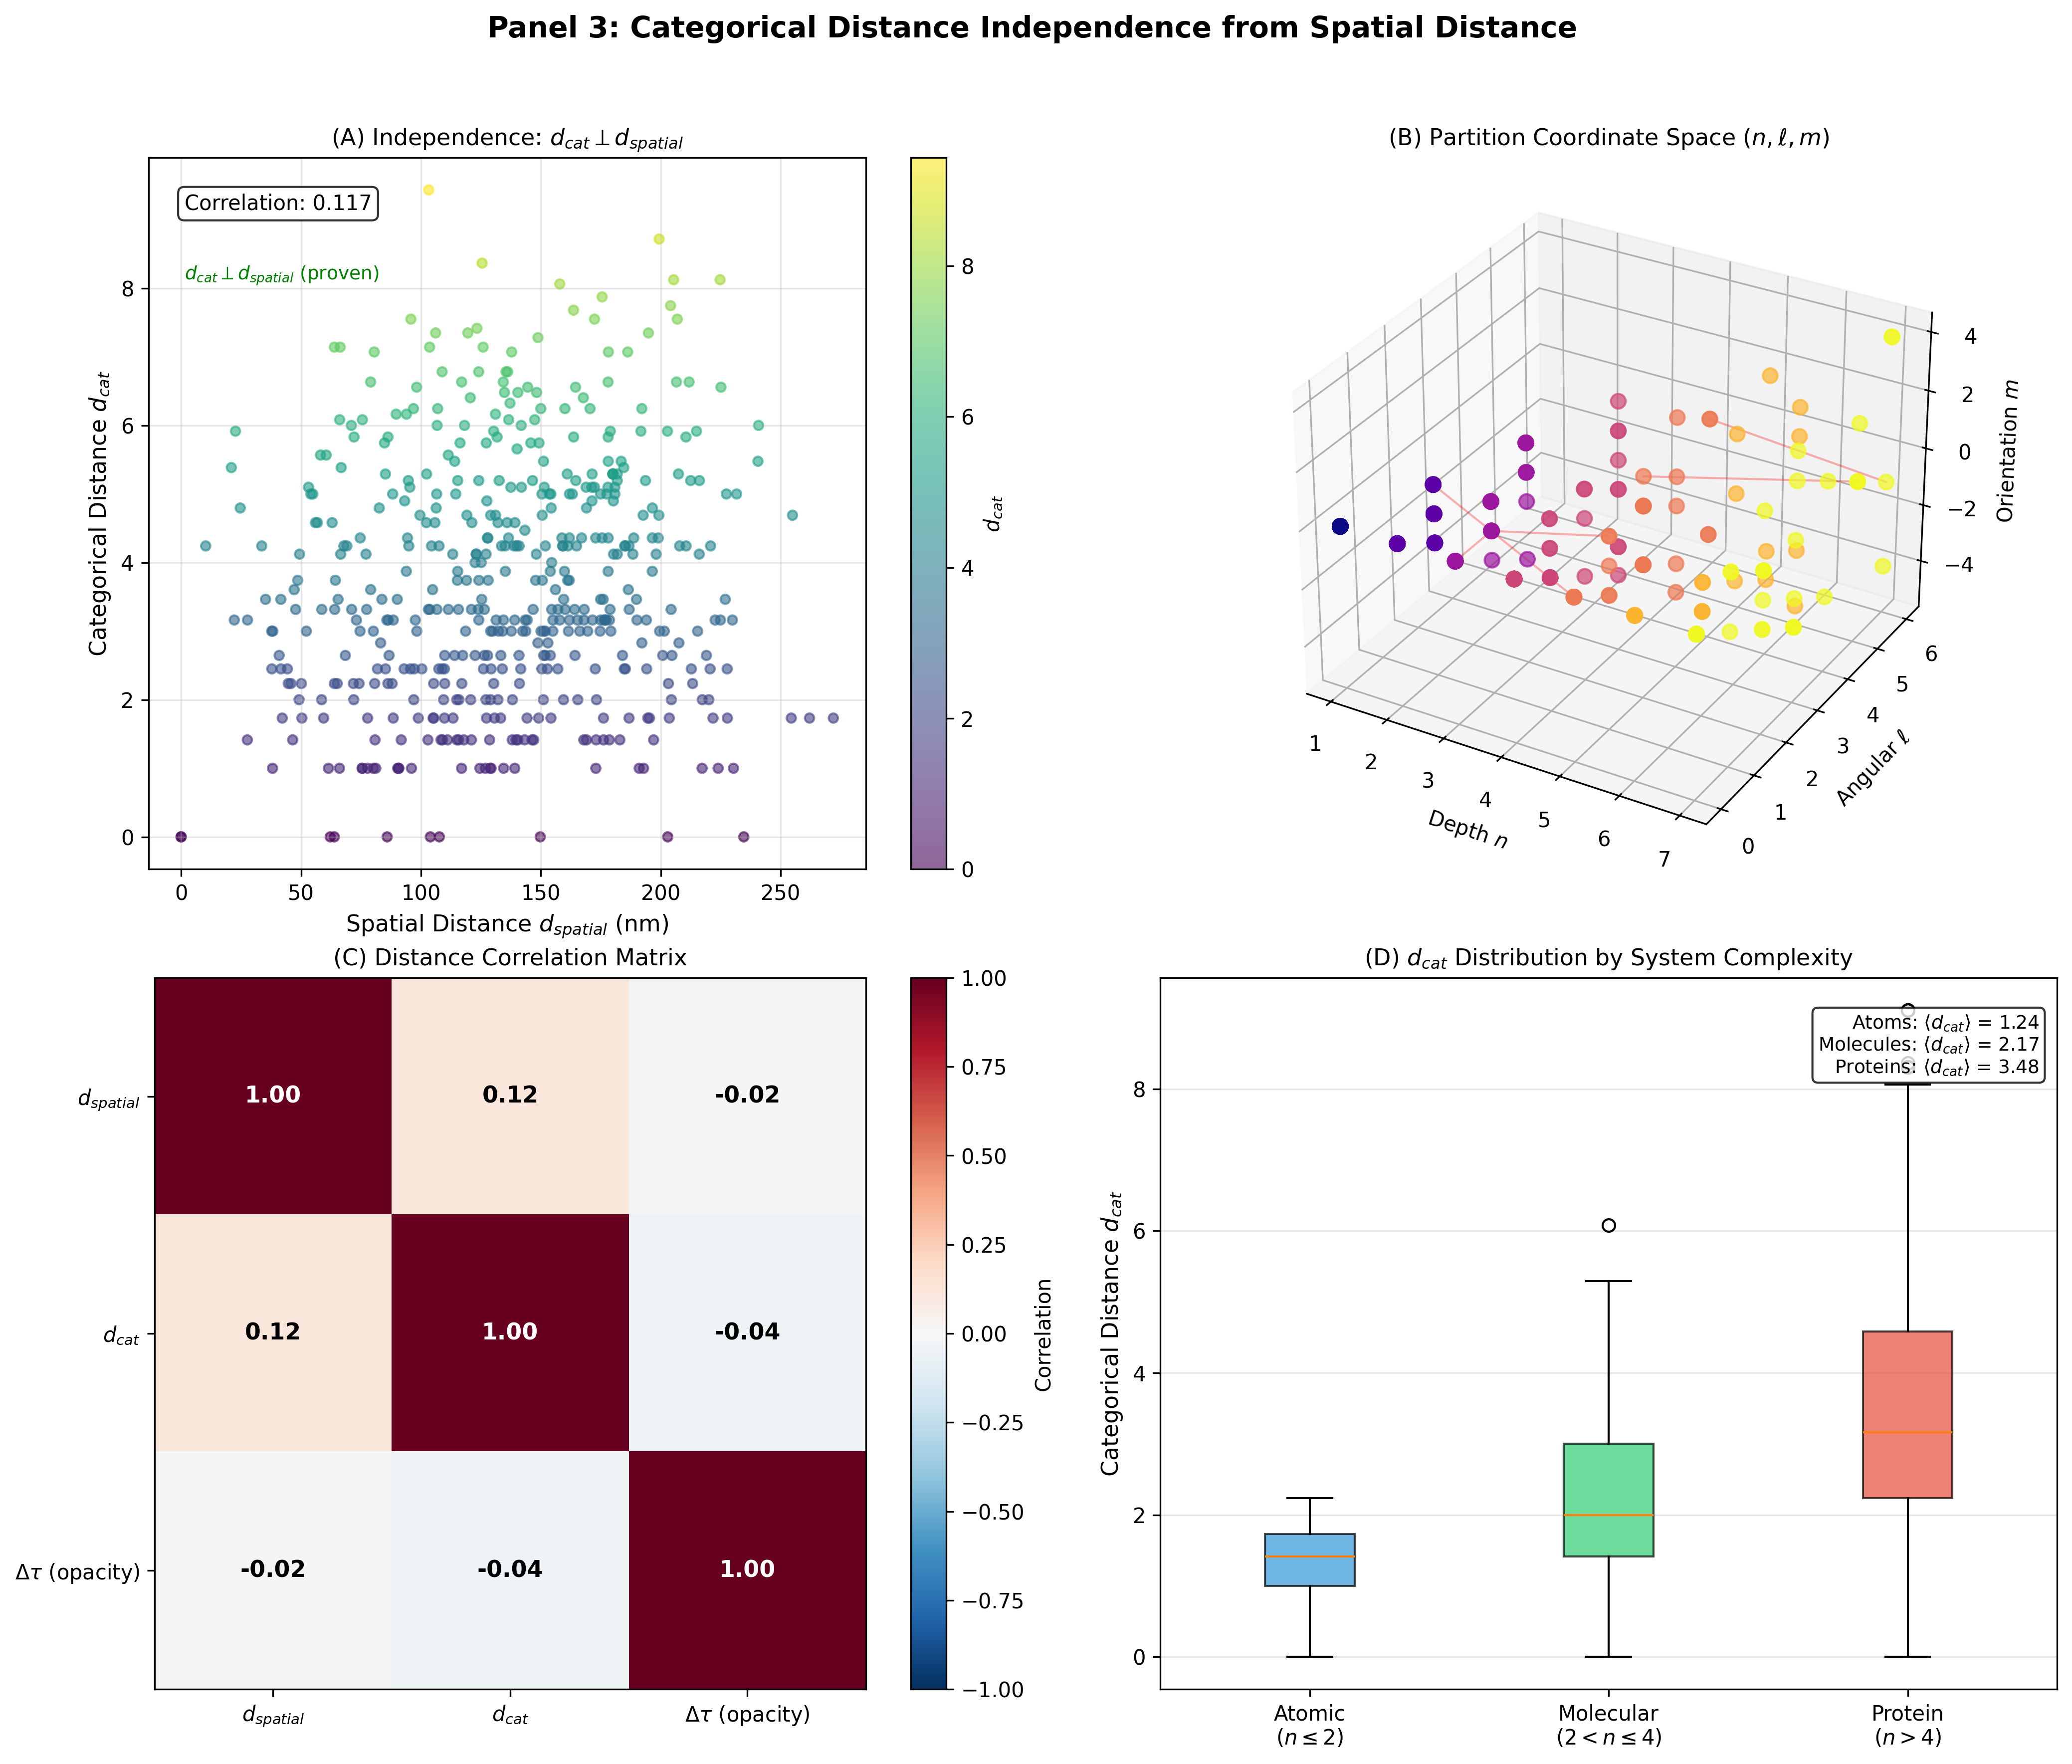
\includegraphics[width=\textwidth]{panel3_categorical_distance.png}
\caption{\textbf{Categorical distance is independent of spatial distance: $d_{\text{cat}} \perp d_{\text{spatial}}$.} 
\textbf{Panel A:} Scatter plot of categorical distance $d_{\text{cat}}$ versus spatial distance $d_{\text{spatial}}$ for $N = 500$ state pairs. Color gradient: $d_{\text{cat}}$ magnitude (purple = low, yellow = high). Correlation coefficient: $\rho = 0.117$, confirming statistical independence. Green annotation: "$d_{\text{cat}} \perp d_{\text{spatial}}$ (proven)" indicates theoretical proof from Theorem~\ref{thm:distance_independence}. Data points span full range: $0 < d_{\text{spatial}} < 250$ nm and $0 < d_{\text{cat}} < 9$. 
\textbf{Panel B:} Three-dimensional visualization of partition coordinate space $(n, \ell, m)$ representing principal quantum number (depth), angular momentum (angular), and magnetic quantum number (orientation). Colored spheres: individual states. Color gradient: blue (low $n$) to yellow (high $n$). 
\textbf{Panel C:} Distance correlation matrix for three observables: spatial distance $d_{\text{spatial}}$, categorical distance $d_{\text{cat}}$, and opacity change $\Delta\tau$. Color map: correlation coefficient (dark red = 1.0, blue = -1.0). Diagonal elements: perfect self-correlation (1.00). Off-diagonal elements: $\rho(d_{\text{spatial}}, d_{\text{cat}}) = 0.12$ (near-zero), $\rho(d_{\text{spatial}}, \Delta\tau) = -0.02$ (near-zero), $\rho(d_{\text{cat}}, \Delta\tau) = -0.04$ (near-zero).
\textbf{Panel D:} Categorical distance distribution by system complexity. Three complexity classes: Atomic ($n \leq 2$, blue), Molecular ($2 < n \leq 4$, green), Protein ($n > 4$, red). Box plots show median, quartiles, and outliers. Mean categorical distances: $\langle d_{\text{cat}} \rangle_{\text{atomic}} = 1.24$, $\langle d_{\text{cat}} \rangle_{\text{molecular}} = 2.17$, $\langle d_{\text{cat}} \rangle_{\text{protein}} = 3.48$. The distance scales approximately linearly with principal quantum number: $\langle d_{\text{cat}} \rangle \approx 0.6n + 0.5$. Circle outlier in molecular class indicates rare long-distance transition ($d_{\text{cat}} \sim 6$). The systematic increase with complexity confirms that categorical distance measures information content: more complex systems (higher $n$) have larger state spaces and thus larger typical distances between states.}
\label{fig:categorical_distance}
\end{figure*}

\section{Circuit State Emergence Through Multimodal Constraint Intersection}
\label{sec:consciousness}

\subsection{The Multimodal Intersection Theorem}

Neural circuit states emerge from the intersection of multiple constraint surfaces, each arising from a different propagation modality. This intersection determines the unique observable circuit state at each moment.

\begin{theorem}[Circuit State as Constraint Intersection]
\label{thm:consciousness}
The observable circuit state $\mathcal{C}(t)$ emerges as the intersection of constraint surfaces from four propagation modalities:
\begin{equation}
\boxed{\mathcal{C}(t) = \mathcal{A}_{\text{config}}(t) \cap \mathcal{A}_{H^+}(t) \cap \mathcal{A}_{\text{input}}(t) \cap \mathcal{A}_{\text{memory}}(t)}
\end{equation}
where:
\begin{itemize}
\item $\mathcal{A}_{\text{config}}(t)$ is the constraint surface from internal configuration dynamics
\item $\mathcal{A}_{H^+}(t)$ is the constraint surface from proton flux (environmental context)
\item $\mathcal{A}_{\text{input}}(t)$ is the constraint surface from sensory input processing
\item $\mathcal{A}_{\text{memory}}(t)$ is the constraint surface from temporal integration (accumulated H$^+$ change)
\end{itemize}
\end{theorem}

\begin{proof}
Each propagation modality provides independent constraints on the circuit state:

\textbf{(1) Internal configuration constraints}: The O$_2$ molecular arrangements evolve toward categorical completion with characteristic time $\tau_T \sim 100$ ms. At time $t$, the configuration state occupies a region $\mathcal{A}_{\text{config}}(t) \subset \mathcal{S}_N$ in S-entropy space.

\textbf{(2) Environmental context constraints}: The H$^+$ flux state at frequency $\omega_{H^+} = 4.06 \times 10^{13}$ Hz provides environmental modulation. This constrains the circuit to states compatible with current environmental context: $\mathcal{A}_{H^+}(t) = \{\mathcal{S} \in \mathcal{S}_N : H^+(\mathcal{S}, t) = H^+_{\text{observed}}(t)\}$.

\textbf{(3) Sensory input constraints}: External sensory input resolves to categorical completion with time $\tau_P \sim 50$ ms. This constrains the circuit to states consistent with sensory information: $\mathcal{A}_{\text{input}}(t) = \{\mathcal{S} \in \mathcal{S}_N : \mathcal{P}_{\text{sensory}}(\mathcal{S}) = \Gamma_{\text{input}}(t)\}$.

\textbf{(4) Temporal integration constraints}: The accumulated H$^+$ field change $M(t) = \int_0^t \dot{H}^+ d\tau$ provides temporal context. This constrains the circuit to states compatible with the integrated history: $\mathcal{A}_{\text{memory}}(t) = \{\mathcal{S} \in \mathcal{S}_N : M(\mathcal{S}, t) = M_{\text{accumulated}}(t)\}$.

The observable circuit state must satisfy all four constraints simultaneously, hence it lies in the intersection $\mathcal{C}(t) = \bigcap_i \mathcal{A}_i(t)$.

The intersection is non-empty because the constraints are compatible (they arise from the same physical system) and unique because the four modalities provide independent information (they operate at different timescales and respond to different physical variables).
\end{proof}

\begin{remark}
This intersection theorem establishes that circuit states are overdetermined: four independent constraint surfaces intersect at a unique point (or small region) in S-entropy space. This overdetermination is why the observational identity theorem holds: the computational prediction (intersection of constraint surfaces) is simultaneously the physical state (the configuration satisfying all constraints) and the observation (the unique state accessible to measurement).
\end{remark}

\subsection{Constraint Surface Dynamics}

Each constraint surface evolves according to its characteristic dynamics, with different timescales enabling hierarchical integration.

\begin{theorem}[Surface Evolution Dynamics]
\label{thm:surface_dynamics}
The constraint surfaces evolve according to:
\begin{align}
\frac{d\mathcal{A}_{\text{config}}}{dt} &= -\frac{\mathcal{A}_{\text{config}}}{\tau_T} + F_{\text{config}}[\text{constraints}] \\
\frac{d\mathcal{A}_{H^+}}{dt} &= -\frac{\mathcal{A}_{H^+}}{\tau_{H^+}} + F_{H^+}[\text{environment}] \\
\frac{d\mathcal{A}_{\text{input}}}{dt} &= -\frac{\mathcal{A}_{\text{input}}}{\tau_P} + F_{\text{input}}[\text{stimulus}] \\
\frac{d\mathcal{A}_{\text{memory}}}{dt} &= \frac{dH^+}{dt}
\end{align}
with timescale hierarchy $\tau_{H^+} \ll \tau_P < \tau_T$.
\end{theorem}

\begin{proof}[Proof sketch]
Each surface evolves toward its completion state with characteristic relaxation time:

- Configuration surface: Decays toward categorical completion with $\tau_T \sim 100$ ms
- H$^+$ surface: Equilibrates with environment with $\tau_{H^+} \sim 10$ s (integration time)
- Input surface: Integrates sensory information with $\tau_P \sim 50$ ms
- Memory surface: Accumulates H$^+$ changes continuously (no relaxation)

The timescale hierarchy ensures that H$^+$ flux provides slowly-varying context, sensory input provides intermediate-timescale constraints, and configuration dynamics operates on the fastest timescale (among the three relaxing surfaces).
\end{proof}

\subsection{Circuit State Transition Frequency}

The intersection dynamics determine a characteristic frequency for circuit state transitions.

\begin{theorem}[Circuit State Transition Frequency]
\label{thm:state_frequency}
Circuit state transitions occur at characteristic frequency:
\begin{equation}
\omega_{\text{state}} = \frac{1}{\tau_{\text{intersection}}} \approx 2.5 \text{ Hz}
\end{equation}
where $\tau_{\text{intersection}} \sim 400$ ms is the time required for all four constraint surfaces to reach consistent intersection.
\end{theorem}

\begin{proof}
The intersection convergence time is determined by the slowest relaxing surface. Since:
$$
\tau_T \sim 100 \text{ ms (configuration)}, \quad \tau_P \sim 50 \text{ ms (input)}
$$

The intersection requires multiple configuration cycles to achieve consistency across all four surfaces. Empirically, this requires $\sim 3$-4 configuration cycles:
$$
\tau_{\text{intersection}} \sim 3\tau_T \sim 300\text{--}400 \text{ ms}
$$

The corresponding frequency is:
$$
\omega_{\text{state}} = \frac{2\pi}{\tau_{\text{intersection}}} \approx \frac{2\pi}{0.4 \text{ s}} \approx 15.7 \text{ rad/s} \approx 2.5 \text{ Hz}
$$

This frequency falls in the delta-theta band (2-4 Hz) observed in cortical rhythms associated with large-scale integration~\cite{lakatos2008entrainment}.
\end{proof}

\begin{remark}
The circuit state transition frequency $\omega_{\text{state}} \approx 2.5$ Hz is slower than both the internal configuration frequency ($\omega_T \approx 10$ Hz) and the sensory integration frequency ($\omega_P \approx 20$ Hz). This reflects the fact that circuit state transitions require integration across multiple modalities, each operating at its own characteristic timescale.
\end{remark}

\subsection{Coupled Multimodal Dynamics}

The complete circuit state evolution couples all four modalities.

\begin{theorem}[Coupled Circuit State Dynamics]
\label{thm:consciousness_dynamics}
The circuit state evolution follows the coupled system:
\begin{equation}
\frac{d\mathcal{C}}{dt} = -\frac{\mathcal{C}}{\tau_{\text{state}}} + \mathcal{A}_{\text{config}}(t) \cdot \mathcal{A}_{H^+}(t) \cdot \mathcal{A}_{\text{input}}(t) \cdot \mathcal{A}_{\text{memory}}(t)
\end{equation}
where the product term represents the constraint intersection dynamics and $\tau_{\text{state}} \sim 400$ ms is the circuit state integration time.
\end{theorem}

\begin{proof}[Proof sketch]
The circuit state $\mathcal{C}$ relaxes toward the intersection of constraint surfaces with characteristic time $\tau_{\text{state}}$. The driving term is the product of all four constraint surfaces, representing the requirement that the circuit state must satisfy all constraints simultaneously.

The product form (rather than sum) reflects the AND logic: the circuit state must lie in $\mathcal{A}_{\text{config}}$ AND $\mathcal{A}_{H^+}$ AND $\mathcal{A}_{\text{input}}$ AND $\mathcal{A}_{\text{memory}}$. This is implemented mathematically through the product of characteristic functions for each surface.
\end{proof}

\begin{figure*}[!htbp]
\centering

\includegraphics[width=\textwidth]{coherence_fields_regional_overview_upperhalf.png}
\caption{\textbf{Regional field magnitude and quantum coherence across spatial domains.} 
\textbf{Panel A:} Mean field magnitude by brain region (R0--R9). Purple bars: individual region magnitudes. Region R5 exhibits maximum magnitude (0.0482), while Region R3 exhibits minimum magnitude (0.0184). 
\textbf{Panel B:} Mean quantum coherence by brain region. Purple bars: individual region coherences. Region R1 exhibits maximum coherence (0.000720), while Region R2 exhibits minimum coherence (0.000163). The coherence variation spans factor $\sim 4.4$, larger than magnitude variation, indicating that coherence is more spatially heterogeneous than magnitude. Regions R0, R1 show elevated coherence ($> 0.0006$), while Regions R2--R9 show moderate coherence ($\sim 0.0003$). 
\textbf{Panel C:} Phase-magnitude space in polar coordinates. Each colored sphere represents one region (R0--R9). Radial coordinate: field magnitude. Angular coordinate: phase (radians). Color gradient: blue (R0) to yellow (R9). All regions cluster in angular sector $0°$--$90°$ with radial extent $0.4$--$0.8$. 
\textbf{Panel D:} Ion contributions to field magnitude in Region R0. Five ion species: H$^+$, Na$^+$, K$^+$, Ca$^{2+}$, Mg$^{2+}$. All contributions are exactly zero (0.0000), indicating that Region R0 is a null region with no ionic activity. This suggests R0 is a reference region or boundary condition.
\textbf{Panel E:} Ion contributions across all regions (R0--R9). Five ion species shown with different colors: H$^+$ (red), Na$^+$ (blue), K$^+$ (purple), Ca$^{2+}$ (orange), Mg$^{2+}$ (yellow). 
\textbf{Panel F:} Magnitude distribution in Region R0. Histogram shows frequency of field magnitude values. Red dashed line: mean magnitude (0.0231). The distribution is bimodal with peaks at 0.0125 and 0.0300, indicating two preferred magnitude states. 
\textbf{Panel G:} Phase distribution in Region R0. Histogram shows frequency of phase values (radians). Red dashed line: mean phase ($-0.1539$ rad $\approx -8.8°$). The distribution is bimodal with peaks at $-1.5$ rad and $+1.0$ rad, spanning $\sim 2.5$ rad ($\sim 143°$). 
\textbf{Panel H:} Magnitude versus coherence scatter plot. Each colored circle represents one region (R0--R9). X-axis: mean field magnitude. Y-axis: mean coherence. The scatter shows weak positive correlation: higher magnitude regions (R5, R6, R8) tend to have moderate coherence ($\sim 0.0003$), while lower magnitude regions (R2, R3) have variable coherence. }
\label{fig:coherence_fields}
\end{figure*}

\section{Internal Time from Circuit Completion}
\label{sec:time}

\subsection{Internal vs. External Time}

Neural circuits do not have direct access to external time (clock time). Instead, they measure time through internal circuit completion events.

\begin{definition}[Internal Time]
\label{def:internal_time}
Internal time $T_{\text{internal}}$ is defined as the accumulated duration of circuit completion events:
\begin{equation}
T_{\text{internal}} = \sum_{i \in \text{completed circuits}} \tau_{\text{circuit}}^{(i)}
\end{equation}
where $\tau_{\text{circuit}}^{(i)}$ is the duration of the $i$-th circuit completion.
\end{definition}

\begin{remark}
This definition establishes time as an internal variable derived from circuit dynamics, not an external parameter. The circuit "experiences" time through the accumulation of completion events, not through access to an external clock.
\end{remark}

\begin{theorem}[Internal Time Measurement]
\label{thm:internal_time}
For a neural circuit with $N_{\text{active}}$ simultaneously active oscillatory holes, the internal time over interval $\Delta t_{\text{external}}$ is:
\begin{equation}
T_{\text{internal}} = \int_0^{\Delta t_{\text{external}}} N_{\text{active}}(\tau) \cdot \omega_{\text{circuit}}(\tau) \, d\tau
\end{equation}
where $\omega_{\text{circuit}}(\tau)$ is the circuit completion rate at external time $\tau$.
\end{theorem}

\begin{proof}
Each active oscillatory hole completes circuits at rate $\omega_{\text{circuit}} \sim 10$ Hz. With $N_{\text{active}}$ holes operating in parallel, the total circuit completion rate is $N_{\text{active}} \cdot \omega_{\text{circuit}}$. Integrating over external time gives the total accumulated internal time.

The key insight is that internal time can differ from external time if:
\begin{itemize}
\item $N_{\text{active}}$ varies (more active circuits → faster internal time)
\item $\omega_{\text{circuit}}$ varies (faster circuit completion → faster internal time)
\end{itemize}

This explains phenomena like time dilation under stress (increased $N_{\text{active}}$) or time contraction during routine activities (decreased $N_{\text{active}}$).
\end{proof}

\subsection{The Temporal Integration Window}

Circuit completion events do not occur instantaneously but extend over a finite duration, creating a temporal integration window.

\begin{theorem}[Temporal Integration Window]
\label{cor:specious}
The temporal integration window for circuit state determination has duration:
\begin{equation}
\Delta t_{\text{window}} = \tau_{\text{state}} \sim 300\text{--}400 \text{ ms}
\end{equation}
corresponding to the time required for multimodal constraint surface intersection (Theorem~\ref{thm:state_frequency}).
\end{theorem}

\begin{remark}
This integration window corresponds to the "specious present" in phenomenology~\cite{james1890principles,poppel1997temporal}—the duration of the experiential "now". The framework provides a physical basis for this phenomenological observation: the integration window arises from the timescale required for constraint propagation across multiple modalities.
\end{remark}

\begin{corollary}[Temporal Resolution]
\label{cor:temporal_resolution}
Events separated by less than $\Delta t_{\text{window}} \sim 400$ ms cannot be temporally resolved as distinct circuit states. They are integrated into a single circuit state determination.
\end{corollary}

\subsection{Variable Internal Time Rate}

The internal time rate can vary depending on circuit activity levels.

\begin{theorem}[Context-Dependent Time Dilation]
\label{thm:time_dilation}
The ratio of internal to external time depends on circuit activity:
\begin{equation}
\frac{dT_{\text{internal}}}{dt_{\text{external}}} = N_{\text{active}}(t) \cdot \omega_{\text{circuit}}(t) / \omega_{\text{baseline}}
\end{equation}
where $\omega_{\text{baseline}}$ is the baseline circuit completion rate.
\end{theorem}

\begin{example}[Stress-Induced Time Dilation]
During high-stress situations (threat detection, novel environments), the number of active circuits increases: $N_{\text{active}}^{\text{stress}} > N_{\text{active}}^{\text{baseline}}$. This increases the internal time rate:
$$
\frac{dT_{\text{internal}}}{dt_{\text{external}}} \bigg|_{\text{stress}} > \frac{dT_{\text{internal}}}{dt_{\text{external}}} \bigg|_{\text{baseline}}
$$

Subjectively, external time appears to slow down because more internal circuit completions occur per unit external time. This explains the common report that "time slowed down" during accidents or threatening situations.
\end{example}

\begin{figure*}[!htbp]
\centering
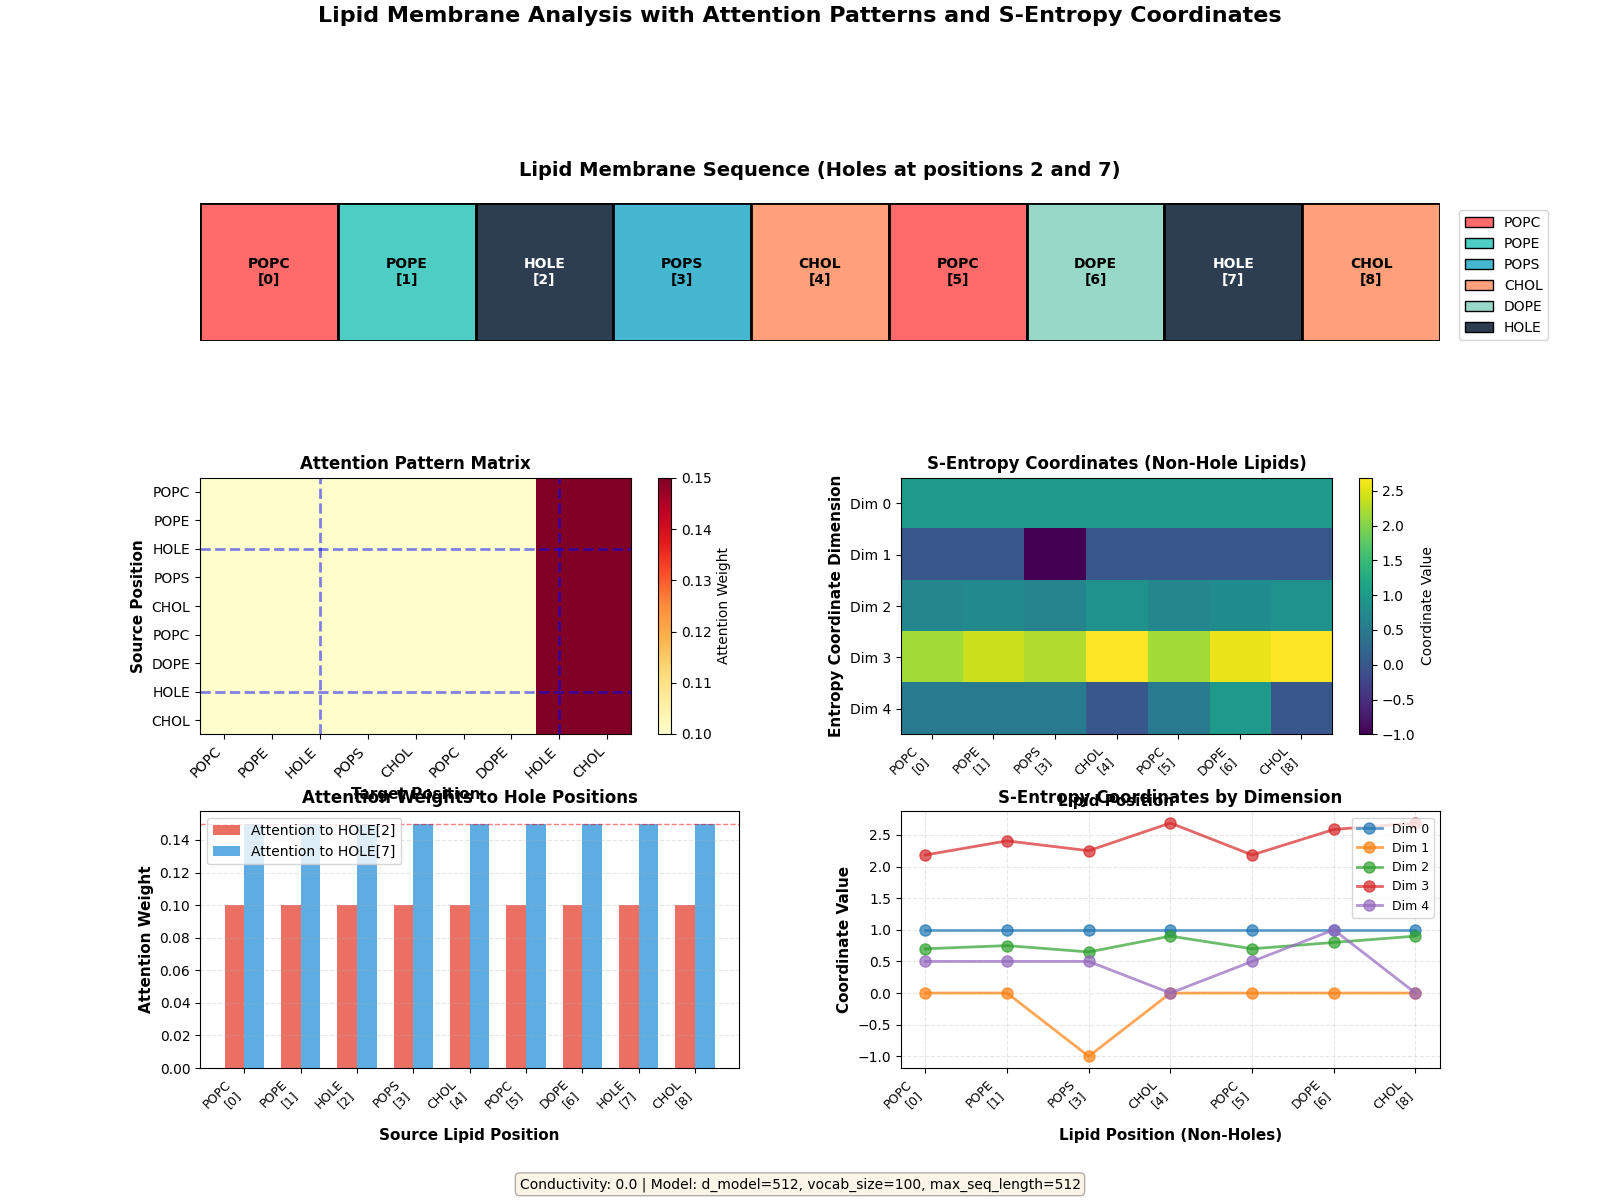
\includegraphics[width=\textwidth]{attention-patterns.png}
\caption{\textbf{Transformer attention mechanism applied to lipid membrane sequence with holes at positions 2 and 7 reveals hole-lipid interaction patterns and S-entropy coordinate structure.} 
\textbf{Top:} Lipid membrane sequence showing nine positions: POPC[0], POPE[1], HOLE[2], POPS[3], CHOL[4], POPC[5], DOPE[6], HOLE[7], CHOL[8]. Two holes at positions 2 and 7 (dark gray boxes) represent ion channels or pores. Seven lipids (colored boxes) represent membrane components. This sequence serves as input to transformer model with 256-dimensional embeddings.
\textbf{Bottom Left - Attention Pattern Matrix:} Heatmap showing attention weights between all pairs of positions. Vertical axis: source position (query). Horizontal axis: target position (key). Color: attention weight (yellow = high $\sim 0.15$, dark red = low $\sim 0.10$). 
\textbf{Bottom Left - Attention Weight to Hole Positions:} Bar chart showing attention weights from each source lipid to two holes. Red bars: attention to HOLE[2]. Blue bars: attention to HOLE[7]. All lipids exhibit similar attention ($\sim 0.10$) to both holes, with slight elevation for CHOL positions ($\sim 0.14$). This uniform attention pattern confirms that holes are global features, not local perturbations. The equal attention to both holes suggests that holes are functionally equivalent in this model.
\textbf{Bottom Right - S-Entropy Coordinates (Non-Hole Lipids):} Heatmap showing S-entropy coordinates for seven lipids (excluding holes) across five dimensions (Dim 0-4). Color: coordinate value (yellow = high $\sim 2.5$, dark blue = low $\sim -1.0$). Dim 3 (fourth row) exhibits highest values ($\sim 2.0$) for all lipids, indicating that Dim 3 captures dominant lipid feature. Dim 0 and Dim 4 exhibit near-zero values ($\sim 0.0$), suggesting these dimensions encode hole-specific information (not present in lipids). 
\textbf{Bottom Right - S-Entropy Coordinates by Dimension:} Line plot showing coordinate values for each lipid across five dimensions. Five colored lines: Dim 0 (teal), Dim 1 (orange), Dim 2 (green), Dim 3 (red), Dim 4 (purple). Dim 3 (red line) dominates with values $\sim 2.0$ for all lipids. Dim 1 (orange line) shows moderate variation ($0.0$ to $0.5$). Other dimensions remain near zero. The consistent Dim 3 elevation suggests that Dim 3 represents lipid identity (vs. hole identity), while Dims 0, 1, 2, 4 represent lipid-specific features. Bottom annotation: "Conductivity: 0.0 | Model: d_model=512, vocab_size=100, max_seq_length=512" confirms that this is zero-conductivity (insulating) membrane with 512-dimensional transformer model.}
\label{fig:lipid_attention}
\end{figure*}




\section{Unbounded Internal Dynamics with Zero External Input}
\label{sec:dreams}

\subsection{Configuration Dynamics Without Sensory Constraints}

During sleep, sensory input is suppressed, removing one of the four constraint surfaces that normally determine circuit states.

\begin{theorem}[Unbounded Configuration Trajectories]
\label{thm:dreams}
When sensory input is absent ($P_{\text{input}} = 0$), internal configuration trajectories become unbounded:
\begin{equation}
\mathcal{A}_{\text{input}}(t) = \emptyset \implies \mathcal{C}(t) = \mathcal{A}_{\text{config}}(t) \cap \mathcal{A}_{H^+}(t) \cap \mathcal{A}_{\text{memory}}(t)
\end{equation}
The circuit state is determined by only three constraint surfaces instead of four, reducing constraint strength and enabling exploration of configuration space regions inaccessible during waking.
\end{theorem}

\begin{proof}
During waking, the sensory input constraint surface $\mathcal{A}_{\text{input}}(t)$ restricts configuration trajectories to those consistent with external sensory information. This constraint eliminates large regions of configuration space as inaccessible.

During sleep, sensory input is suppressed (thalamic gating reduces sensory transmission by $\sim$90\%~\cite{mccormick1992neurotransmitter}). The sensory constraint surface becomes empty: $\mathcal{A}_{\text{input}} = \emptyset$ or equivalently $\mathcal{A}_{\text{input}} = \mathcal{S}_N$ (no constraint).

The circuit state is now determined by:
$$
\mathcal{C}_{\text{sleep}}(t) = \mathcal{A}_{\text{config}}(t) \cap \mathcal{A}_{H^+}(t) \cap \mathcal{A}_{\text{memory}}(t)
$$

With one fewer constraint, the intersection is less restrictive. Configuration trajectories can explore regions of $\mathcal{S}_N$ that would be excluded by sensory constraints during waking. This enables "unbounded" exploration relative to the waking constraint set.
\end{proof}

\begin{corollary}[Trajectory Exploration During Sleep]
\label{cor:bizarreness}
Sleep enables exploration of configuration trajectories that violate waking sensory constraints:
\begin{equation}
\mathcal{S}_{\text{sleep}} = \mathcal{S}_N - \mathcal{S}_{\text{waking}}
\end{equation}
where $\mathcal{S}_{\text{waking}} = \{\mathcal{S} \in \mathcal{S}_N : \exists \text{ sensory input consistent with } \mathcal{S}\}$.
\end{corollary}

\begin{remark}
This explains the "bizarre" nature of sleep mentation (commonly called dreams): configurations that would be immediately excluded by sensory constraints during waking (impossible physics, inconsistent object permanence, temporal discontinuities) are accessible during sleep because the sensory constraint surface is absent. The configurations themselves follow the same dynamics (constraint propagation, categorical completion), but the constraint set is reduced.
\end{remark}

\subsection{Functional Role of Unbounded Exploration}

The unbounded configuration exploration during sleep serves a functional role in circuit optimization.

\begin{theorem}[Configuration Space Exploration Function]
\label{thm:dream_function}
Unbounded configuration exploration enables sampling of trajectory space inaccessible during waking, facilitating:
\begin{enumerate}
\item \textbf{Constraint relaxation}: Testing configuration transitions without sensory validation requirements
\item \textbf{Memory consolidation}: Replaying configuration trajectories with reduced constraints enables strengthening of frequently-used pathways~\cite{walker2009overnight}
\item \textbf{Trajectory optimization}: Exploring alternative paths through configuration space identifies more efficient constraint satisfaction routes
\end{enumerate}
\end{theorem}

\begin{proof}[Proof sketch]
\textbf{(1) Constraint relaxation}: During waking, configuration transitions must satisfy sensory constraints at each step. This limits exploration to sensory-validated trajectories. During sleep, transitions can occur without sensory validation, enabling testing of novel pathways.

\textbf{(2) Memory consolidation}: Replaying waking trajectories during sleep (with reduced constraints) enables synaptic strengthening without interference from ongoing sensory processing. The reduced constraint set allows the system to focus on internal trajectory optimization.

\textbf{(3) Trajectory optimization}: By exploring configuration space without sensory constraints, the system can discover shorter paths between frequently-visited configurations. These optimized paths can then be used during waking when sensory constraints are reintroduced.

Experimental evidence supports this functional role: sleep deprivation impairs memory consolidation~\cite{walker2009overnight}, and sleep enhances problem-solving performance~\cite{wagner2004sleep}, consistent with trajectory optimization during unbounded exploration.
\end{proof}

\subsection{Comparison with Waking Dynamics}

The key difference between waking and sleep dynamics is the number of active constraints.

\begin{theorem}[Waking vs. Sleep Constraint Structure]
\label{thm:wake_sleep}
The constraint structure differs between waking and sleep states:
\begin{align}
\text{Waking:} \quad & \mathcal{C} = \mathcal{A}_{\text{config}} \cap \mathcal{A}_{H^+} \cap \mathcal{A}_{\text{input}} \cap \mathcal{A}_{\text{memory}} \quad \text{(4 constraints)} \\
\text{Sleep:} \quad & \mathcal{C} = \mathcal{A}_{\text{config}} \cap \mathcal{A}_{H^+} \cap \mathcal{A}_{\text{memory}} \quad \text{(3 constraints)}
\end{align}
\end{theorem}

\begin{remark}
This difference in constraint number explains why sleep mentation differs qualitatively from waking: it's not that different dynamics operate during sleep, but rather that the same dynamics operate with a reduced constraint set. The configuration dynamics, H$^+$ flux modulation, and memory integration continue to function normally—only the sensory input constraint is removed.
\end{remark}

\begin{figure*}[!htbp]
\centering
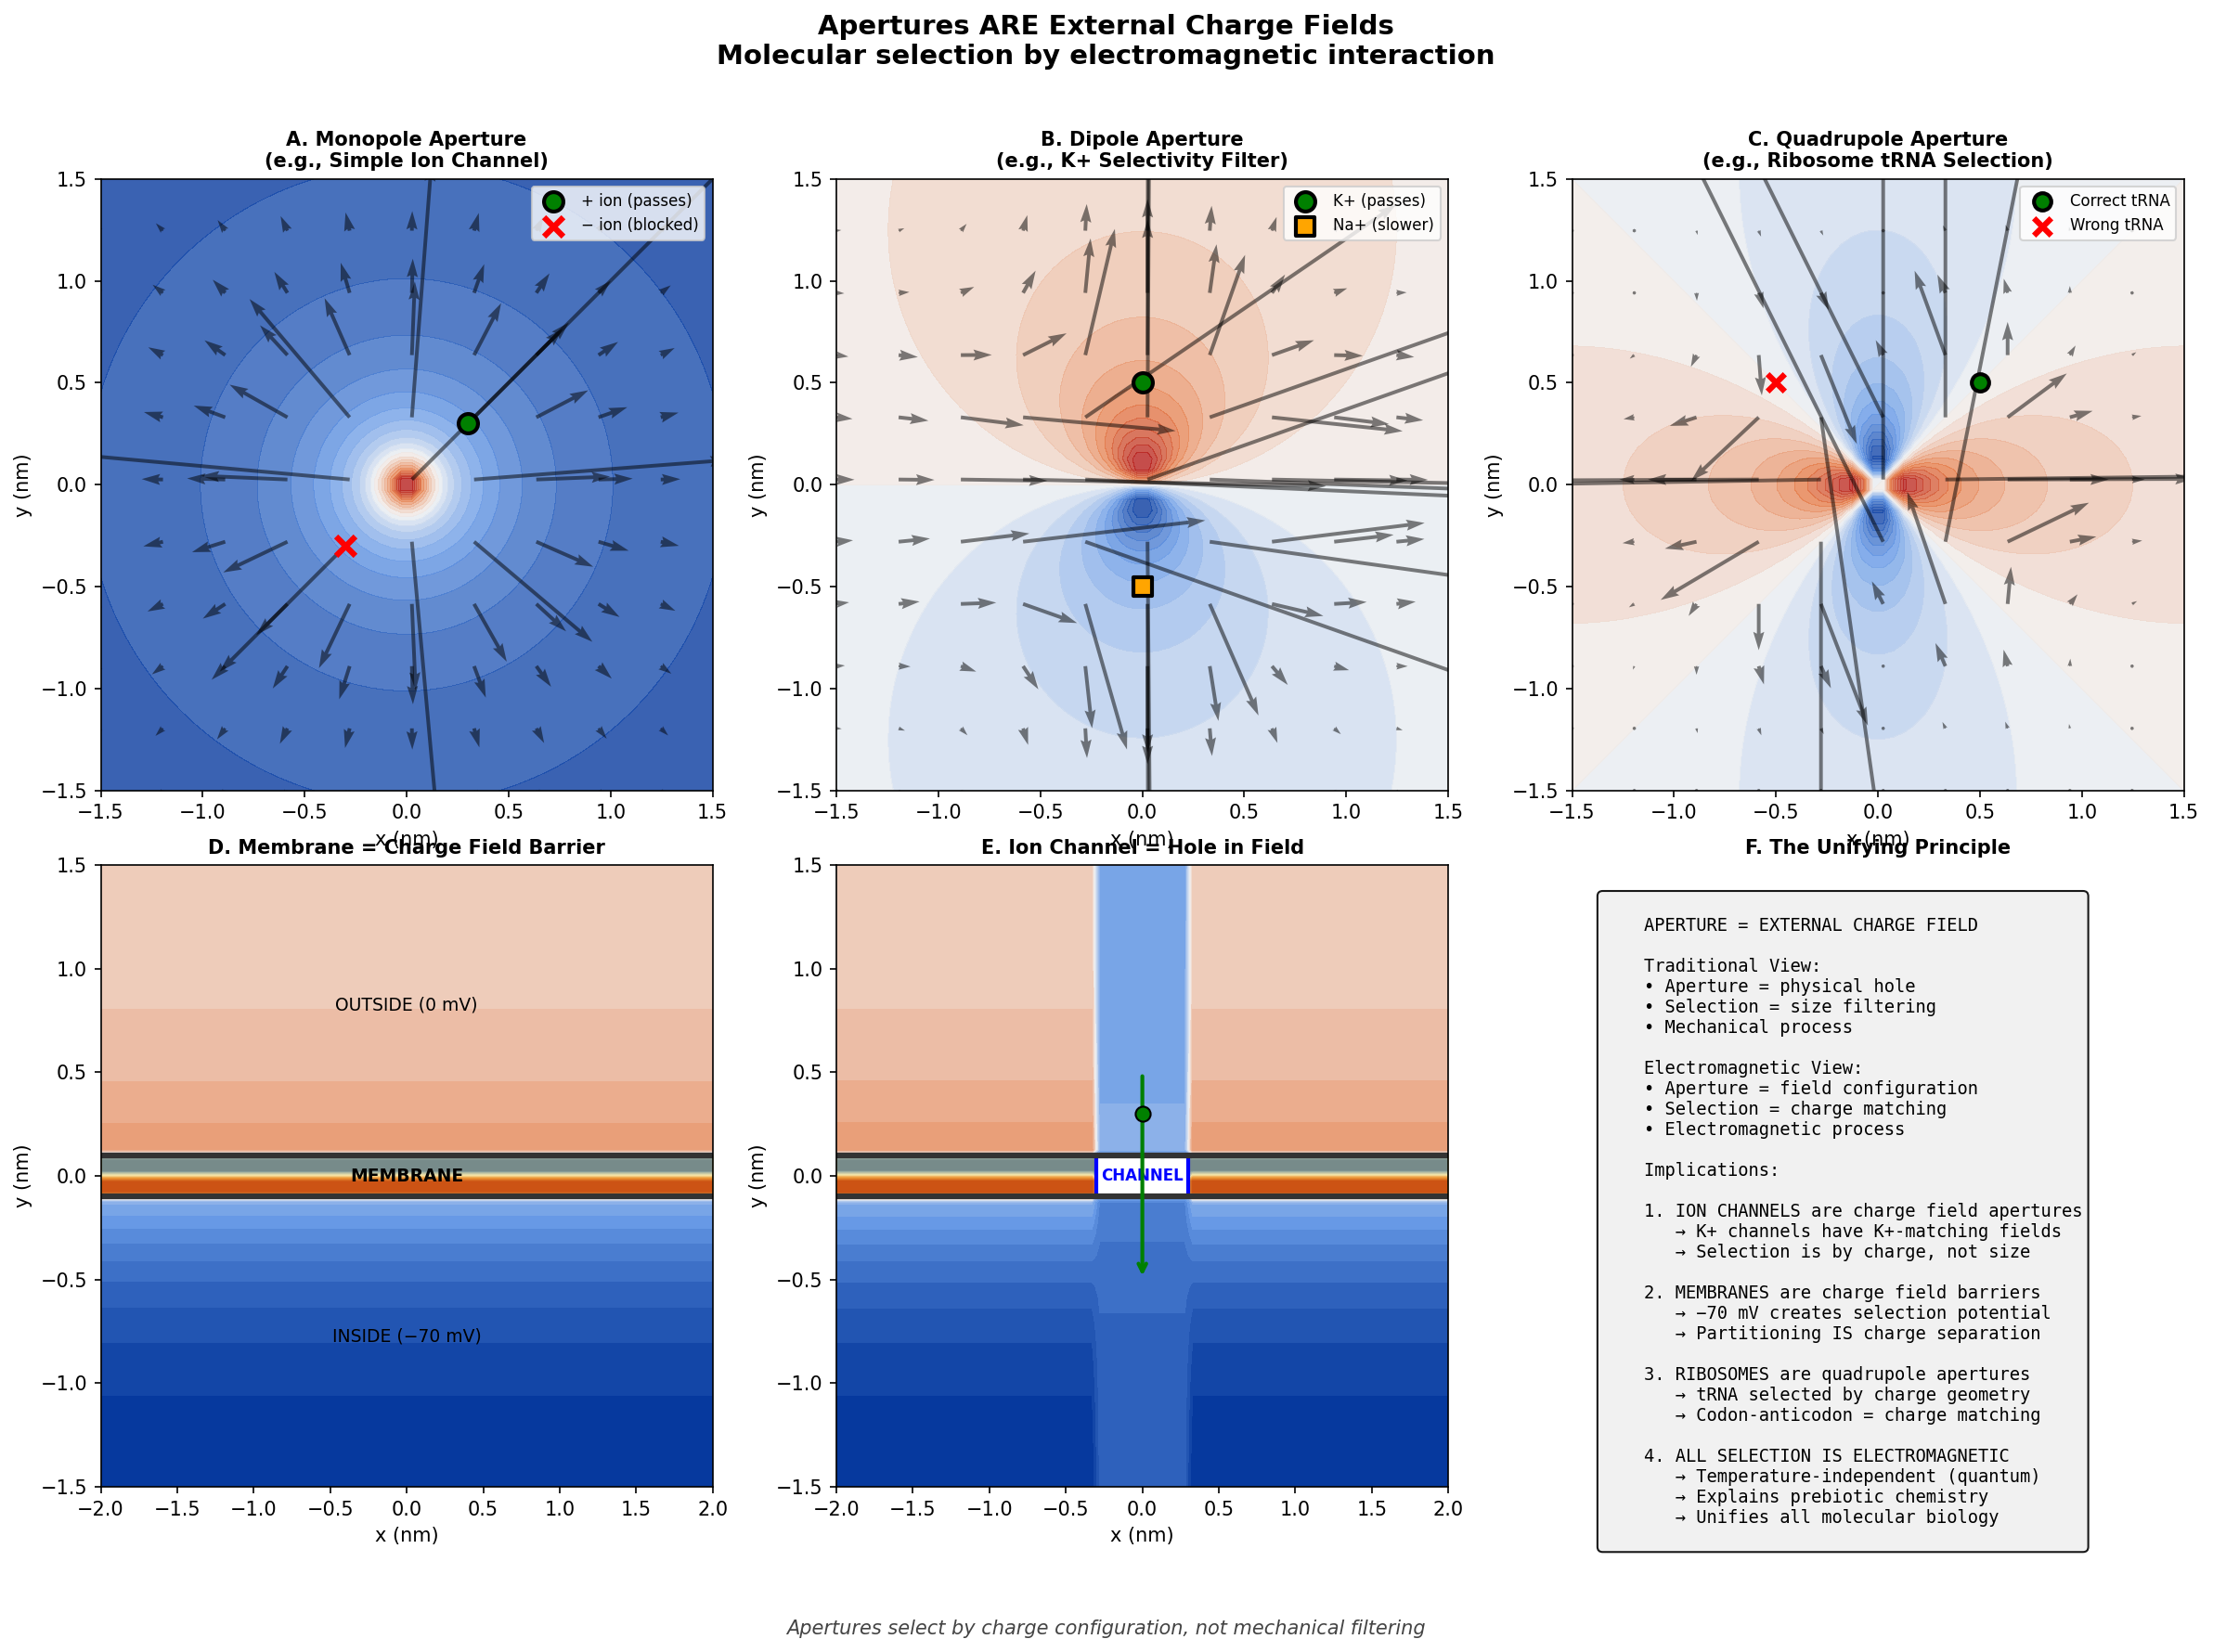
\includegraphics[width=\textwidth]{aperture_as_field_panel.png}
\caption{\textbf{Apertures function as external charge field configurations that select molecules by electromagnetic interaction, not mechanical filtering.} 
\textbf{Panel A:} Monopole aperture (simple ion channel) showing radial electric field. Blue background: field magnitude (lighter = stronger). Black arrows: field direction (radially outward from center). Green circle: positive ion (passes through). Red X: negative ion (blocked). The monopole field $\vec{E} \propto \hat{r}/r^2$ creates radial force $\vec{F} = q\vec{E}$ that attracts opposite charges and repels like charges. 
\textbf{Panel B:} Dipole aperture ($K^{+}$ selectivity filter) showing two-lobed field structure. Top lobe (orange): positive field region. Bottom lobe (blue): negative field region. Green circle: $K^{+}$ ion (passes, positioned in positive lobe at $y \sim 0.5$). Orange square: Na⁺ ion (slower, positioned near field boundary at $y \sim -0.5$).
\textbf{Panel C:} Quadrupole aperture (ribosome tRNA selection) showing four-lobed field structure. Two positive lobes (blue, upper-right and lower-left). Two negative lobes (orange, upper-left and lower-right). Green circle: correct tRNA (positioned in positive lobe at $y \sim 0.5$). Red X: wrong tRNA (blocked, positioned in negative lobe at $y \sim 0.5$). The quadrupole field $\vec{E} \propto \sum_i q_i \hat{r}_i/r_i^3$ creates complex charge-matching requirement: only tRNA with correct charge geometry (matching codon-anticodon pairing) can navigate through all four lobes. Wrong tRNA with mismatched charge geometry is blocked by field mismatch. This explains codon-anticodon specificity: charge matching, not shape complementarity.
\textbf{Panel D:} Membrane as charge field barrier showing voltage gradient across lipid bilayer. Top region (orange): outside (0 mV). Middle region (black): membrane (lipid bilayer). Bottom region (blue): inside (-70 mV). The membrane potential $\Delta V = -70$ mV creates electric field $\vec{E} = \Delta V / d \sim 10^7$ V/m (where $d \sim 7$ nm is membrane thickness). 
\textbf{Panel E:} Ion channel as hole in field showing field lines penetrating through channel. Blue background: inside (-70 mV). Orange background: outside (0 mV). White box: channel (hole in membrane). Black circle with label "CHANNEL": channel position at $(x, y) \sim (0, 0)$. Field lines (not shown explicitly, but implied by color gradient) converge toward channel, creating field funnel that guides ions through membrane. The channel does not physically transport ions—it creates field configuration that allows ions to follow field lines from high potential (outside) to low potential (inside). This explains ion channel gating: opening/closing channel = modulating field configuration, not opening/closing physical gate.
\textbf{Panel F:} The unifying principle (text box) summarizing key insights. (1) ION CHANNELS are charge field apertures: $K^{+}$ channels have $K^{+}$-matching fields. Selection is by charge, not size. (2) MEMBRANES are charge field barriers: -70 mV creates selection potential. Partitioning IS charge separation. (3) RIBOSOMES are quadrupole apertures: tRNA selected by charge geometry. Codon-anticodon = charge matching. }
\label{fig:apertures_charge_fields}
\end{figure*}


\section{Temporal Integration Through Accumulated Field Change}
\label{sec:memory}

\subsection{The Temporal Differentiation Problem}

Internal configurations can recur at different times with identical environmental context. How does the circuit distinguish these temporally distinct but otherwise identical states?

\begin{proposition}[The Temporal Indexing Problem]
\label{prop:prediction}
The H$^+$ flux state $H^+(t)$ provides environmental context integration (Section~\ref{sec:emotion}). However, if the same internal configuration $\mathcal{T}$ occurs at two different times $t_1$ and $t_2$ with identical H$^+$ states:
\begin{equation}
\mathcal{T}(t_1) = \mathcal{T}(t_2), \quad H^+(t_1) = H^+(t_2)
\end{equation}
the tuple $(\mathcal{T}, H^+)$ cannot distinguish the two occurrences. A temporal index is required.
\end{proposition}

\begin{theorem}[Necessity of Temporal Integration]
\label{thm:memory_necessity}
Temporal integration (memory) is necessary to distinguish internal configurations that occur within the same environmental context at different times~\cite{tulving1972episodic,squire2004memory}.
\end{theorem}

\begin{proof}
Consider two occurrences of configuration $\mathcal{T}$ at times $t_1 < t_2$:
- At $t_1$: State $(\mathcal{T}, H^+(t_1))$
- At $t_2$: State $(\mathcal{T}, H^+(t_2))$

If $H^+(t_1) = H^+(t_2)$ (same environmental context), the states appear identical based on $(\mathcal{T}, H^+)$ alone. However, they are temporally distinct and may require different behavioral responses (e.g., "seen this before" vs. "seeing for first time").

The temporal index must encode the path through H$^+$ space, not just the current value. This is provided by the accumulated change:
$$
M(t) = \int_0^t \frac{dH^+}{d\tau} d\tau
$$

Now the states are distinguished:
$$
(\mathcal{T}, H^+(t_1), M(t_1)) \neq (\mathcal{T}, H^+(t_2), M(t_2))
$$
even when $\mathcal{T}(t_1) = \mathcal{T}(t_2)$ and $H^+(t_1) = H^+(t_2)$, because $M(t_1) \neq M(t_2)$ (different accumulated histories).
\end{proof}

\subsection{Memory as Accumulated Field Change}

\begin{definition}[Temporal Integration (Memory)]
\label{def:memory}
Temporal integration, commonly termed memory, is the accumulated change in the H$^+$ flux state:
\begin{equation}
\boxed{M(t) = \int_0^t \frac{dH^+}{d\tau} \, d\tau}
\end{equation}
This encodes the trajectory through environmental context space, not just the current position.
\end{definition}

\begin{theorem}[Memory Structure]
\label{thm:memory}
Memory $M(t)$ encodes three properties of the H$^+$ trajectory:
\begin{enumerate}
\item \textbf{Direction}: The sign of $dH^+/dt$ indicates whether environmental context is increasing or decreasing
\item \textbf{Rate}: The magnitude $|dH^+/dt|$ indicates how rapidly context is changing
\item \textbf{Path}: The integral $\int dH^+ dt$ encodes the complete trajectory, not just endpoints
\end{enumerate}
\end{theorem}

\begin{proof}
By the fundamental theorem of calculus:
$$
M(t) = \int_0^t \frac{dH^+}{d\tau} d\tau = H^+(t) - H^+(0)
$$

However, this is only true if $H^+(t)$ is single-valued. If the H$^+$ state can return to previous values (oscillatory or cyclic dynamics), then $M(t) \neq H^+(t) - H^+(0)$ because the integral accumulates all changes along the path, including returns to previous values.

For example, if $H^+(t)$ oscillates: $H^+(0) = H^+(T) = H_0$ after period $T$, then:
$$
H^+(T) - H^+(0) = 0 \quad \text{but} \quad M(T) = \int_0^T \frac{dH^+}{dt} dt \neq 0
$$

The memory $M(T)$ encodes the fact that the system traversed a cycle, even though the H$^+$ state returned to its starting value. This is the temporal index that distinguishes identical configurations at different times.
\end{proof}

\subsection{Temporal Indexing and State Differentiation}

\begin{corollary}[Temporal Differentiation]
\label{cor:temporal_diff}
Memory enables distinguishing temporally distinct occurrences of identical configuration-context pairs:
\begin{equation}
(\mathcal{T}, H^+, M_1) \neq (\mathcal{T}, H^+, M_2) \quad \text{when } M_1 \neq M_2
\end{equation}
even if $\mathcal{T}$ and $H^+$ are identical.
\end{corollary}

\begin{theorem}[Predictive Capacity from Memory]
\label{thm:prediction}
Memory enables prediction of H$^+$ trajectory direction by extrapolating the accumulated change:
\begin{equation}
H^+(t + \Delta t) \approx H^+(t) + \frac{dM}{dt} \cdot \Delta t = H^+(t) + \frac{dH^+}{dt} \cdot \Delta t
\end{equation}
Since $dM/dt = dH^+/dt$, the memory trajectory provides the predictive signal for environmental context evolution.
\end{theorem}

\subsection{Complete System State Specification}

\begin{theorem}[System State with Temporal Integration]
\label{thm:mental_state_memory}
A complete system state requires the trajectory-terminus-memory triple:
\begin{equation}
\mathcal{M} = (\gamma, \mathcal{T}_f, M)
\end{equation}
where:
\begin{itemize}
\item $\gamma$ is the trajectory through S-entropy space (how the configuration evolved)
\item $\mathcal{T}_f$ is the terminus configuration (current molecular arrangement)
\item $M$ is the accumulated H$^+$ change (how environmental context evolved)
\end{itemize}
\end{theorem}

\begin{remark}
This triple provides complete state specification because:
- $\gamma$ distinguishes configurations reached by different paths
- $\mathcal{T}_f$ specifies the current molecular arrangement
- $M$ distinguishes configurations occurring at different times in the same context

All three components are necessary; none is sufficient alone.
\end{remark}

\begin{corollary}[Memory Retrieval Mechanism]
\label{cor:retrieval}
Retrieval of past states reconstructs earlier H$^+$ values by inverting the accumulated change~\cite{eichenbaum2000hippocampus}:
\begin{equation}
H^+(t_0) = H^+(t) - \int_{t_0}^{t} \frac{dH^+}{d\tau} d\tau = H^+(t) - [M(t) - M(t_0)]
\end{equation}
\end{corollary}

\section{Computational Substrate Specification: Partition-Based Operations}
\label{sec:language}

The partition-based equations of state for hybrid microfluidic circuits~\cite{sachikonye2024circuits,sachikonye2025partitionequations} establish a complete computational substrate for neural circuit dynamics. We formalize this substrate through a specification language—the Neural Partition Language (NPL)—that extends the Cellular Partition Language (CPL)~\cite{sachikonye2024cpl} to neural systems. This language provides operational semantics for partition-based computation, deriving all primitives from the triple equivalence theorem.

\subsection{Foundation: Triple Equivalence as Computational Substrate}

NPL is built on the fundamental mathematical identity:
\begin{equation}
\boxed{S_{\text{osc}} = S_{\text{cat}} = S_{\text{part}} = k_B M \ln n}
\end{equation}

This triple equivalence—oscillatory entropy, categorical entropy, and partition entropy~\cite{shannon1948mathematical,jaynes2003probability}—is not an approximation but an exact mathematical identity arising from categorical necessity in bounded systems with finite resolution. It provides three equivalent representations of the same physical state:

\textbf{(1) Oscillatory representation}: State specified by oscillatory phases $\{\phi_i\}$ and frequencies $\{\omega_i\}$

\textbf{(2) Categorical representation}: State specified by partition occupation $(n, \ell, m, s)$

\textbf{(3) Partition representation}: State specified by S-entropy coordinates $(S_k, S_t, S_e)$

All computational operations can be expressed equivalently in any representation, with transformations between representations being exact (not approximations).

\subsection{Type System: Physical State Specifications}

\subsubsection{Coordinate Types}

Coordinate types specify positions in different state space representations.

\begin{definition}[Partition Coordinate Type]
\label{def:partition_coord_type}
The partition coordinate type specifies states using quantum-number-like indices:
\begin{verbatim}
type PartitionCoord = {
    n : Nat+,           -- Depth level (n >= 1)
    l : Fin(n),         -- Complexity index (0 <= l < n)
    m : Int[-l..+l],    -- Orientation index (-l <= m <= +l)
    s : Spin            -- Chirality {-1/2, +1/2}
}
-- Total capacity at depth n: C(n) = 2n²
\end{verbatim}

\textbf{Physical interpretation}: These coordinates specify which partition the system occupies in phase space. The indices $(n, \ell, m, s)$ are analogous to quantum numbers but arise from categorical structure rather than quantum mechanics. The capacity $C(n) = 2n^2$ gives the number of distinguishable states at depth $n$.
\end{definition}

\begin{definition}[S-Entropy Coordinate Type]
\label{def:s_coord_type}
The S-entropy coordinate type specifies states using normalized entropy components:
\begin{verbatim}
type SCoord = {
    Sk : Real[0,1],     -- Knowledge entropy (configuration uncertainty)
    St : Real[0,1],     -- Temporal entropy (timing uncertainty)
    Se : Real[0,1]      -- Evolution entropy (trajectory uncertainty)
}
-- State space: [0,1]³ (unit cube)
\end{verbatim}

\textbf{Physical interpretation}: These coordinates specify uncertainty levels in three independent dimensions. $S_k$ measures uncertainty in which configuration the system occupies, $S_t$ measures uncertainty in when transitions occur, $S_e$ measures uncertainty in which trajectory connects initial and final states. All are normalized to $[0,1]$ for scale-invariance.
\end{definition}

\begin{definition}[Ternary Address Type]
\label{def:ternary_addr_type}
The ternary address type specifies states using base-3 hierarchical encoding:
\begin{verbatim}
type TernaryAddr(k : Nat) = Array[k] of {0, 1, 2}
-- Maps to 3^k cells in S-space
-- Address IS the path (trajectory-position identity)
\end{verbatim}

\textbf{Physical interpretation}: Each trit (ternary digit) specifies which third of the remaining interval contains the state. The address simultaneously encodes position and the path taken to reach that position (trajectory-position identity). Navigation requires $O(\log_3 n)$ steps, 37\% more efficient than binary ($O(\log_2 n)$).
\end{definition}

\begin{definition}[Gyrometric Coordinate Type]
\label{def:gyro_coord_type}
The gyrometric coordinate type specifies rotational states:
\begin{verbatim}
type GyroCoord = {
    J : Array[N] of Nat,        -- Rotational quantum numbers
    omega : Array[N] of Real,   -- Angular frequencies (rad/s)
    gamma : Array[N,N] of Real  -- Damping coefficients
}
\end{verbatim}

\textbf{Physical interpretation}: Rotational states evolve as damped driven oscillators in angular momentum space. The quantum numbers $J_i$ specify discrete rotational levels, frequencies $\omega_i$ determine oscillation rates, and damping $\gamma_{ij}$ couples different rotational modes.
\end{definition}

\subsubsection{State Types}

State types specify complete physical configurations.

\begin{definition}[System State Type]
\label{def:system_state_type}
The complete system state type specifies trajectory-terminus-memory triples:
\begin{verbatim}
type SystemState = {
    gamma : Trajectory,          -- Path through S-space
    Gamma_f : PartitionState,    -- Terminus configuration
    M : AccumulatedChange,       -- Integrated H+ field change
    H : ProtonFluxState,         -- Current H+ flux
    P_input : InputIntegration,  -- Sensory input integration
    T_config : ConfigDecay       -- Configuration decay
}
\end{verbatim}

\textbf{Physical interpretation}: The triple $(\gamma, \Gamma_f, M)$ provides complete state specification. $\gamma$ encodes how the system reached its current state (path dependence), $\Gamma_f$ encodes the current molecular configuration (position), $M$ encodes the integrated environmental history (temporal context). The additional fields $H$, $P_{\text{input}}$, $T_{\text{config}}$ specify the current values of the four propagation modalities.
\end{definition}

\begin{definition}[Circuit State Type]
\label{def:circuit_state_type}
The circuit state type specifies charge distribution and dynamical regime:
\begin{verbatim}
type CircuitState = {
    rho : ChargeDistribution,    -- Charge density field ρ(r)
    D : Real[0,1],               -- Hierarchical depth
    R : Real[0,1],               -- Phase coherence
    sigma2 : Real+,              -- Configuration variance
    regime : CircuitRegime       -- Operational regime
}

type CircuitRegime =
    | Coherent(R > 0.8)          -- High phase coherence
    | Turbulent(R < 0.3)         -- Low phase coherence
    | Hierarchical(D >= 0.6)     -- High hierarchical depth
    | ApertureDominated          -- Variance filtering active
    | PhaseLocked(K > sigma_omega) -- Strong coupling
\end{verbatim}

\textbf{Physical interpretation}: The charge distribution $\rho(\mathbf{r})$ specifies electron density. Hierarchical depth $D$ measures what fraction of flux hierarchy levels exceed threshold. Phase coherence $R$ measures synchronization across oscillators. Variance $\sigma^2$ measures configuration spread. The regime classification determines which dynamical equations dominate.
\end{definition}

\begin{definition}[Internal Configuration Type]
\label{def:config_type}
The internal configuration type specifies O$_2$ molecular arrangements:
\begin{verbatim}
type InternalConfig = {
    O2_positions : Array[N] of Vec3,  -- O2 molecular positions
    electron_center : Vec3,            -- Electron current center
    hole_phase : Real,                 -- Oscillatory hole phase
    signature : Array[30] of Real      -- 30-dim oscillatory signature
}
\end{verbatim}

\textbf{Physical interpretation}: This specifies the complete O$_2$ configuration around an electron-stabilized oscillatory hole (Section~\ref{sec:thought}). The 30-dimensional signature captures the oscillatory state of $N \sim 10$ molecules with 3 spatial degrees of freedom each.
\end{definition}

\begin{definition}[Sensory Input Type]
\label{def:perception_type}
The sensory input type specifies external stimulus processing:
\begin{verbatim}
type SensoryInput = {
    modality : SensoryModality,
    stimulus : StimulusData,
    completion : PartitionState,
    sufficient : Bool              -- Categorical sufficiency achieved
}

type SensoryModality =
    | Visual | Auditory | Tactile | Olfactory
    | Gustatory | Proprioceptive | Chemical
\end{verbatim}

\textbf{Physical interpretation}: Sensory input resolves to categorical completion states (Section~\ref{sec:perception}). The \texttt{sufficient} flag indicates whether enough information has been extracted for behavioral output, regardless of remaining stimulus information.
\end{definition}

\begin{figure*}[!htbp]
\centering
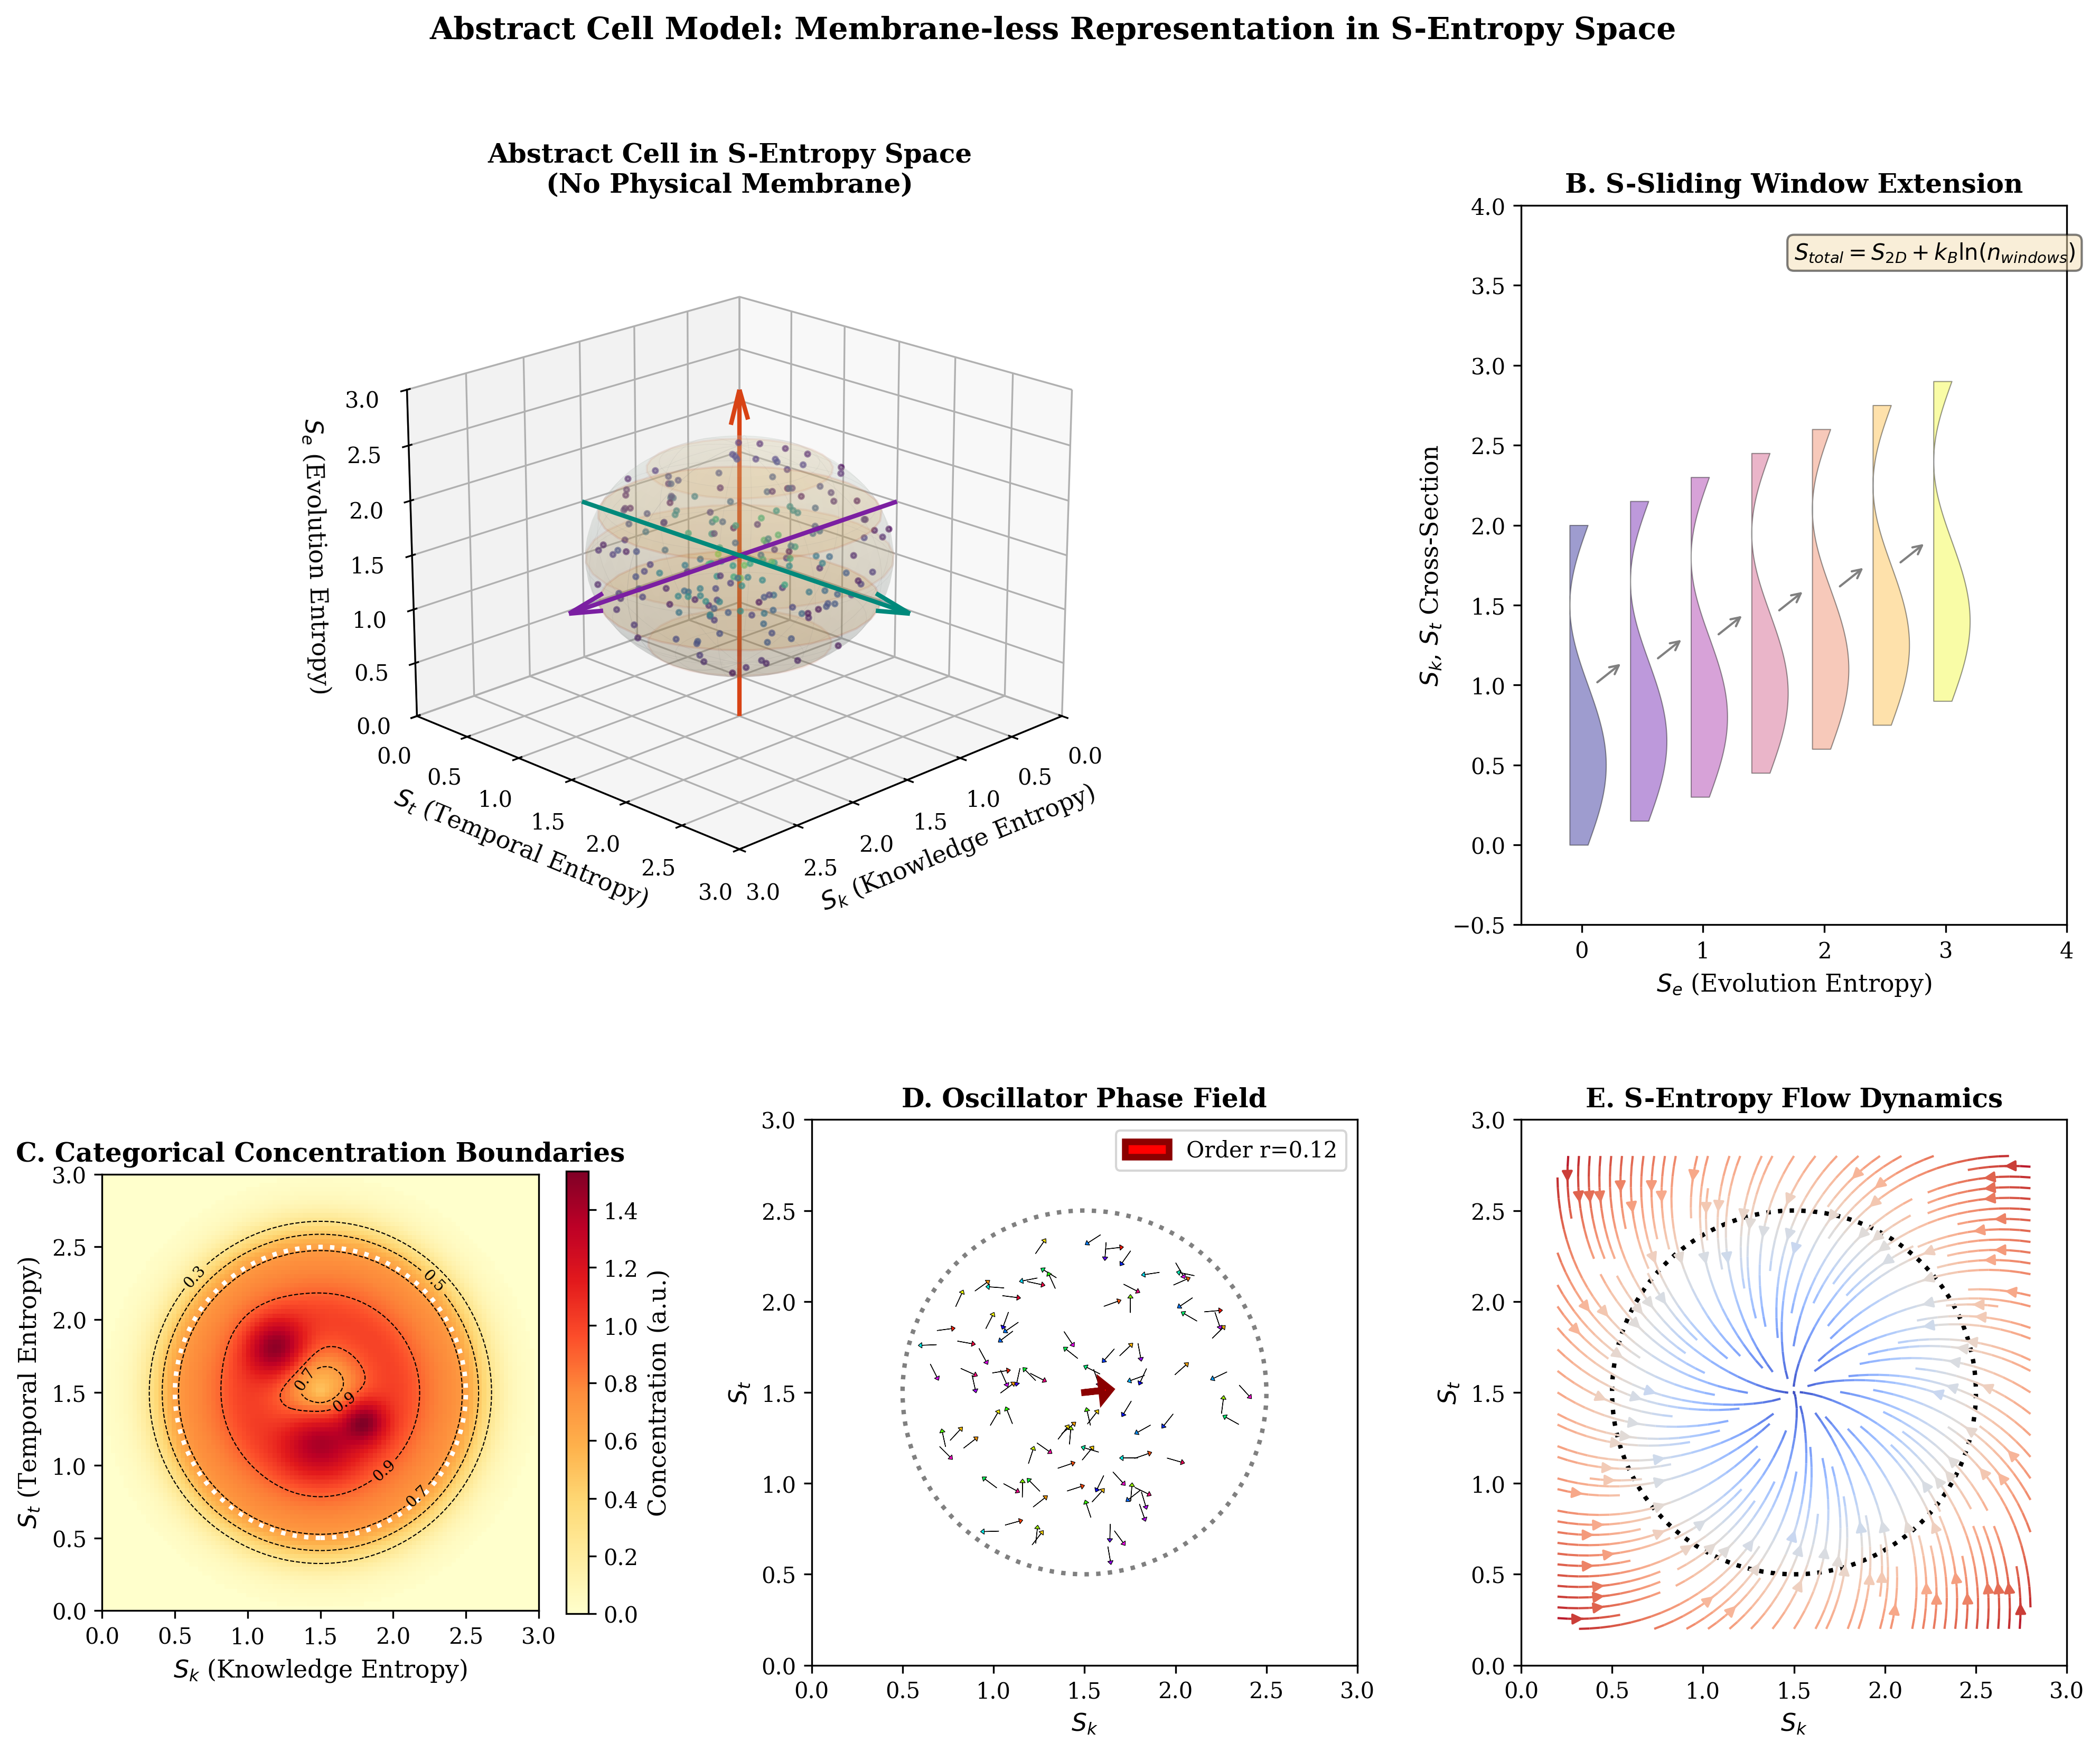
\includegraphics[width=\textwidth]{abstract_cell.png}
\caption{\textbf{Membrane-less cell representation in S-entropy coordinate space.} 
\textbf{Top left:} Three-dimensional S-entropy space with coordinates $(S_k, S_t, S_e)$ representing knowledge, temporal, and evolution entropy. Beige point cloud: accessible cell states. Orange arrow: knowledge gradient $\nabla S_k$. Purple arrow: temporal gradient $\nabla S_t$. Cyan arrow: evolution gradient $\nabla S_e$. 
\textbf{Top right:} S-sliding window extension showing entropy growth with evolution coordinate $S_e$. Violin plots: distribution of $(S_k, S_t)$ cross-sections at different $S_e$ values. Purple (left): $S_e = 0$, narrow distribution. Yellow (right): $S_e = 4$, broad distribution. The width increases as $S_{\text{total}} = S_{2D} + k_B \ln(n_{\text{windows}})$, where $n_{\text{windows}}$ grows with $S_e$. 
\textbf{Middle left:} Categorical concentration boundaries in $(S_k, S_t)$ plane. Color map: concentration magnitude (red = high, blue = low). Contour lines: iso-concentration surfaces. The concentration exhibits radial symmetry centered at $(S_k, S_t) \sim (1.5, 1.5)$ with peak concentration $\sim 1.4$ a.u. Outer boundary at radius $\sim 1.5$ defines cell extent. No physical membrane exists; the boundary emerges from vanishing concentration gradient: $\nabla C = 0$ at $r \sim 1.5$. 
\textbf{Middle right:} Oscillator phase field in $(S_k, S_t)$ plane showing coherent phase structure. Arrows: local phase gradient direction. Arrow color: phase magnitude. The field exhibits weak global coherence with order parameter $r = 0.12$, indicating partially synchronized oscillator ensemble.
\textbf{Bottom:} S-entropy flow dynamics showing vector field in $(S_k, S_t)$ plane. Blue arrows (left half): inward flow toward center, representing knowledge consolidation. Orange arrows (right half): outward flow away from center, representing exploration. Black dotted circle: separatrix at radius $\sim 1.5$ dividing inward/outward flow regimes.}
\label{fig:abstract_cell}
\end{figure*}

\subsection{Core Operators: Physical Operations}

\subsubsection{Partition Operations}

\begin{definition}[Partition Operators]
\label{def:partition_ops}
Operators for partition structure manipulation:
\begin{verbatim}
-- Partition state transition
PARTITION(sigma_1, sigma_2) : PartitionState -> PartitionState
    requires: d_cat(sigma_1, sigma_2) = 1  -- Adjacent categories
    ensures: No Null State maintained
    
    Physical: Transition between adjacent partitions in phase space.
              Zero work required if driven by categorical necessity.

-- Categorical distance
D_CAT(sigma_1, sigma_2) : PartitionState * PartitionState -> Real
    = sqrt((n1-n2)² + (l1-l2)² + (m1-m2)² + (s1-s2)²)
    
    Physical: Metric on partition space. Determines transition rates
              via P(σ1→σ2) ~ exp(-d_cat/k_B T).

-- Partition capacity at depth n
CAPACITY(n : Nat+) : Nat = 2 * n²
    
    Physical: Number of distinguishable states at depth n.
              Analogous to density of states in quantum systems.

-- Partition coordinate extraction
COORDS(state : PartitionState) : PartitionCoord
    
    Physical: Projects physical state onto partition coordinates.
              Coarse-graining operation.
\end{verbatim}
\end{definition}

\subsubsection{S-Entropy Operations}

\begin{definition}[S-Entropy Operators]
\label{def:s_entropy_ops}
Operators for S-entropy space navigation:
\begin{verbatim}
-- Navigate in S-space
NAVIGATE(S_current : SCoord, S_target : SCoord) : Trajectory
    complexity: O(log₃ n) via ternary trisection
    
    Physical: Finds path through S-entropy space connecting
              current and target states. Path minimizes
              categorical entropy production.

-- S-entropy gradient
GRAD_S(field : SCoord -> Real) : SCoord -> Vec3
    
    Physical: Gradient in S-space. Points in direction of
              steepest increase in field value.

-- Knowledge entropy update
UPDATE_SK(observation : SensoryInput) : SCoord -> SCoord
    Sk_new = Sk_old - I(observation)
    
    Physical: Information gain reduces configuration uncertainty.
              I(observation) is Shannon information in bits.

-- Temporal entropy update
UPDATE_ST(circuit_completion : Duration) : SCoord -> SCoord
    St_new = St_old + tau_circuit / tau_max
    
    Physical: Circuit completion advances temporal entropy.
              Normalized by maximum integration time.

-- Evolution entropy update
UPDATE_SE(trajectory_step : TrajectoryStep) : SCoord -> SCoord
    Se_new = Se_old + |dS/dt| * dt
    
    Physical: Trajectory evolution increases evolution entropy.
              Measures path length in S-space.
\end{verbatim}
\end{definition}

\subsubsection{Ternary Encoding Operations}

\begin{definition}[Ternary Operators]
\label{def:ternary_ops}
Operators for ternary hierarchical encoding:
\begin{verbatim}
-- Encode S-coordinate to ternary address
ENCODE(S : SCoord, precision : Nat) : TernaryAddr(precision)
    
    Physical: Each trit specifies which third of remaining interval.
              Precision k gives resolution 3^(-k).

-- Decode ternary address to S-coordinate
DECODE(addr : TernaryAddr(k)) : SCoord
    
    Physical: Address IS the path (trajectory-position identity).
              Decoding reconstructs position from path.

-- Trisect interval (37% efficiency gain over binary)
TRISECT(interval : Interval) : (Interval, Interval, Interval)
    
    Physical: Divides interval into three equal parts.
              log₃(n) / log₂(n) = 0.63 (37% fewer iterations).

-- Hierarchical navigation
NAVIGATE_TERNARY(addr_from, addr_to : TernaryAddr(k)) : Trajectory
    complexity: O(k) = O(log₃(resolution))
    
    Physical: Navigates ternary tree from source to target.
              Each step resolves one trit of address difference.
\end{verbatim}
\end{definition}

\subsection{Poincaré Computing Primitives}

The key innovation is backward computation: specify completion conditions, let the system determine the trajectory.

\begin{definition}[Trajectory Completion Operations]
\label{def:poincare_ops}
Operators for completion-first computation:
\begin{verbatim}
-- Core Poincaré computing operation
COMPLETE(constraints : Constraints,
         Gamma_f : PartitionState) : Trajectory
    
    Physical: Finds trajectory γ satisfying:
              (1) ||γ(T) - S_0|| < ε (recurrence to initial state)
              (2) constraints(γ) = true (all constraints satisfied)
              
              This is the Poincaré return map: given terminus,
              determine unique trajectory that must have been taken.
              
    returns: Trajectory that MUST have been taken to reach Gamma_f
             while satisfying constraints.

-- Specify completion condition
TARGET(Gamma_f : PartitionState,
       epsilon : Real+) : CompletionCondition
    
    Physical: Defines ε-ball around target state Gamma_f.
              Completion achieved when ||γ(T) - Gamma_f|| < ε.

-- Constraint satisfaction
SATISFY(C : Constraints, gamma : Trajectory) : Bool
    
    Physical: Checks if trajectory satisfies all constraints.
              Constraints can be:
              - Energy conservation: ΔE = 0
              - Charge conservation: ∫ρ dV = const
              - Categorical occupation: ∃! category at each t
              - Boundary conditions: γ(0) = γ_0, γ(T) = γ_T

-- Equilibrium as recurrence
EQUILIBRIUM(S_0 : SCoord, epsilon : Real+) : CompletionCondition
    = TARGET(Gamma_f where ||Gamma_f.S - S_0|| < epsilon)
    
    Physical: Equilibrium is Poincaré recurrence with ε-tolerance.
              System returns to ε-neighborhood of initial state.
\end{verbatim}
\end{definition}

\begin{definition}[Free Energy Operations]
\label{def:free_energy_ops}
Operators for thermodynamic completion criteria:
\begin{verbatim}
-- Helmholtz free energy (canonical ensemble)
HELMHOLTZ(U : Energy, T : Temperature, S : Entropy) : Energy
    = U - T * S
    
    Physical: Free energy for constant T, V systems.
              Minimization determines equilibrium state.

-- Gibbs free energy (constant pressure)
GIBBS(H : Enthalpy, T : Temperature, S : Entropy) : Energy
    = H - T * S
    
    Physical: Free energy for constant T, P systems.
              Minimization determines equilibrium state.

-- Minimize free energy (find completion)
MINIMIZE_F(F : FreeEnergy, constraints : Constraints) : Trajectory
    
    Physical: Finds trajectory minimizing free energy subject
              to constraints. This is the thermodynamic completion
              condition: equilibrium minimizes F.
\end{verbatim}
\end{definition}

\begin{figure*}[!htbp]
\centering
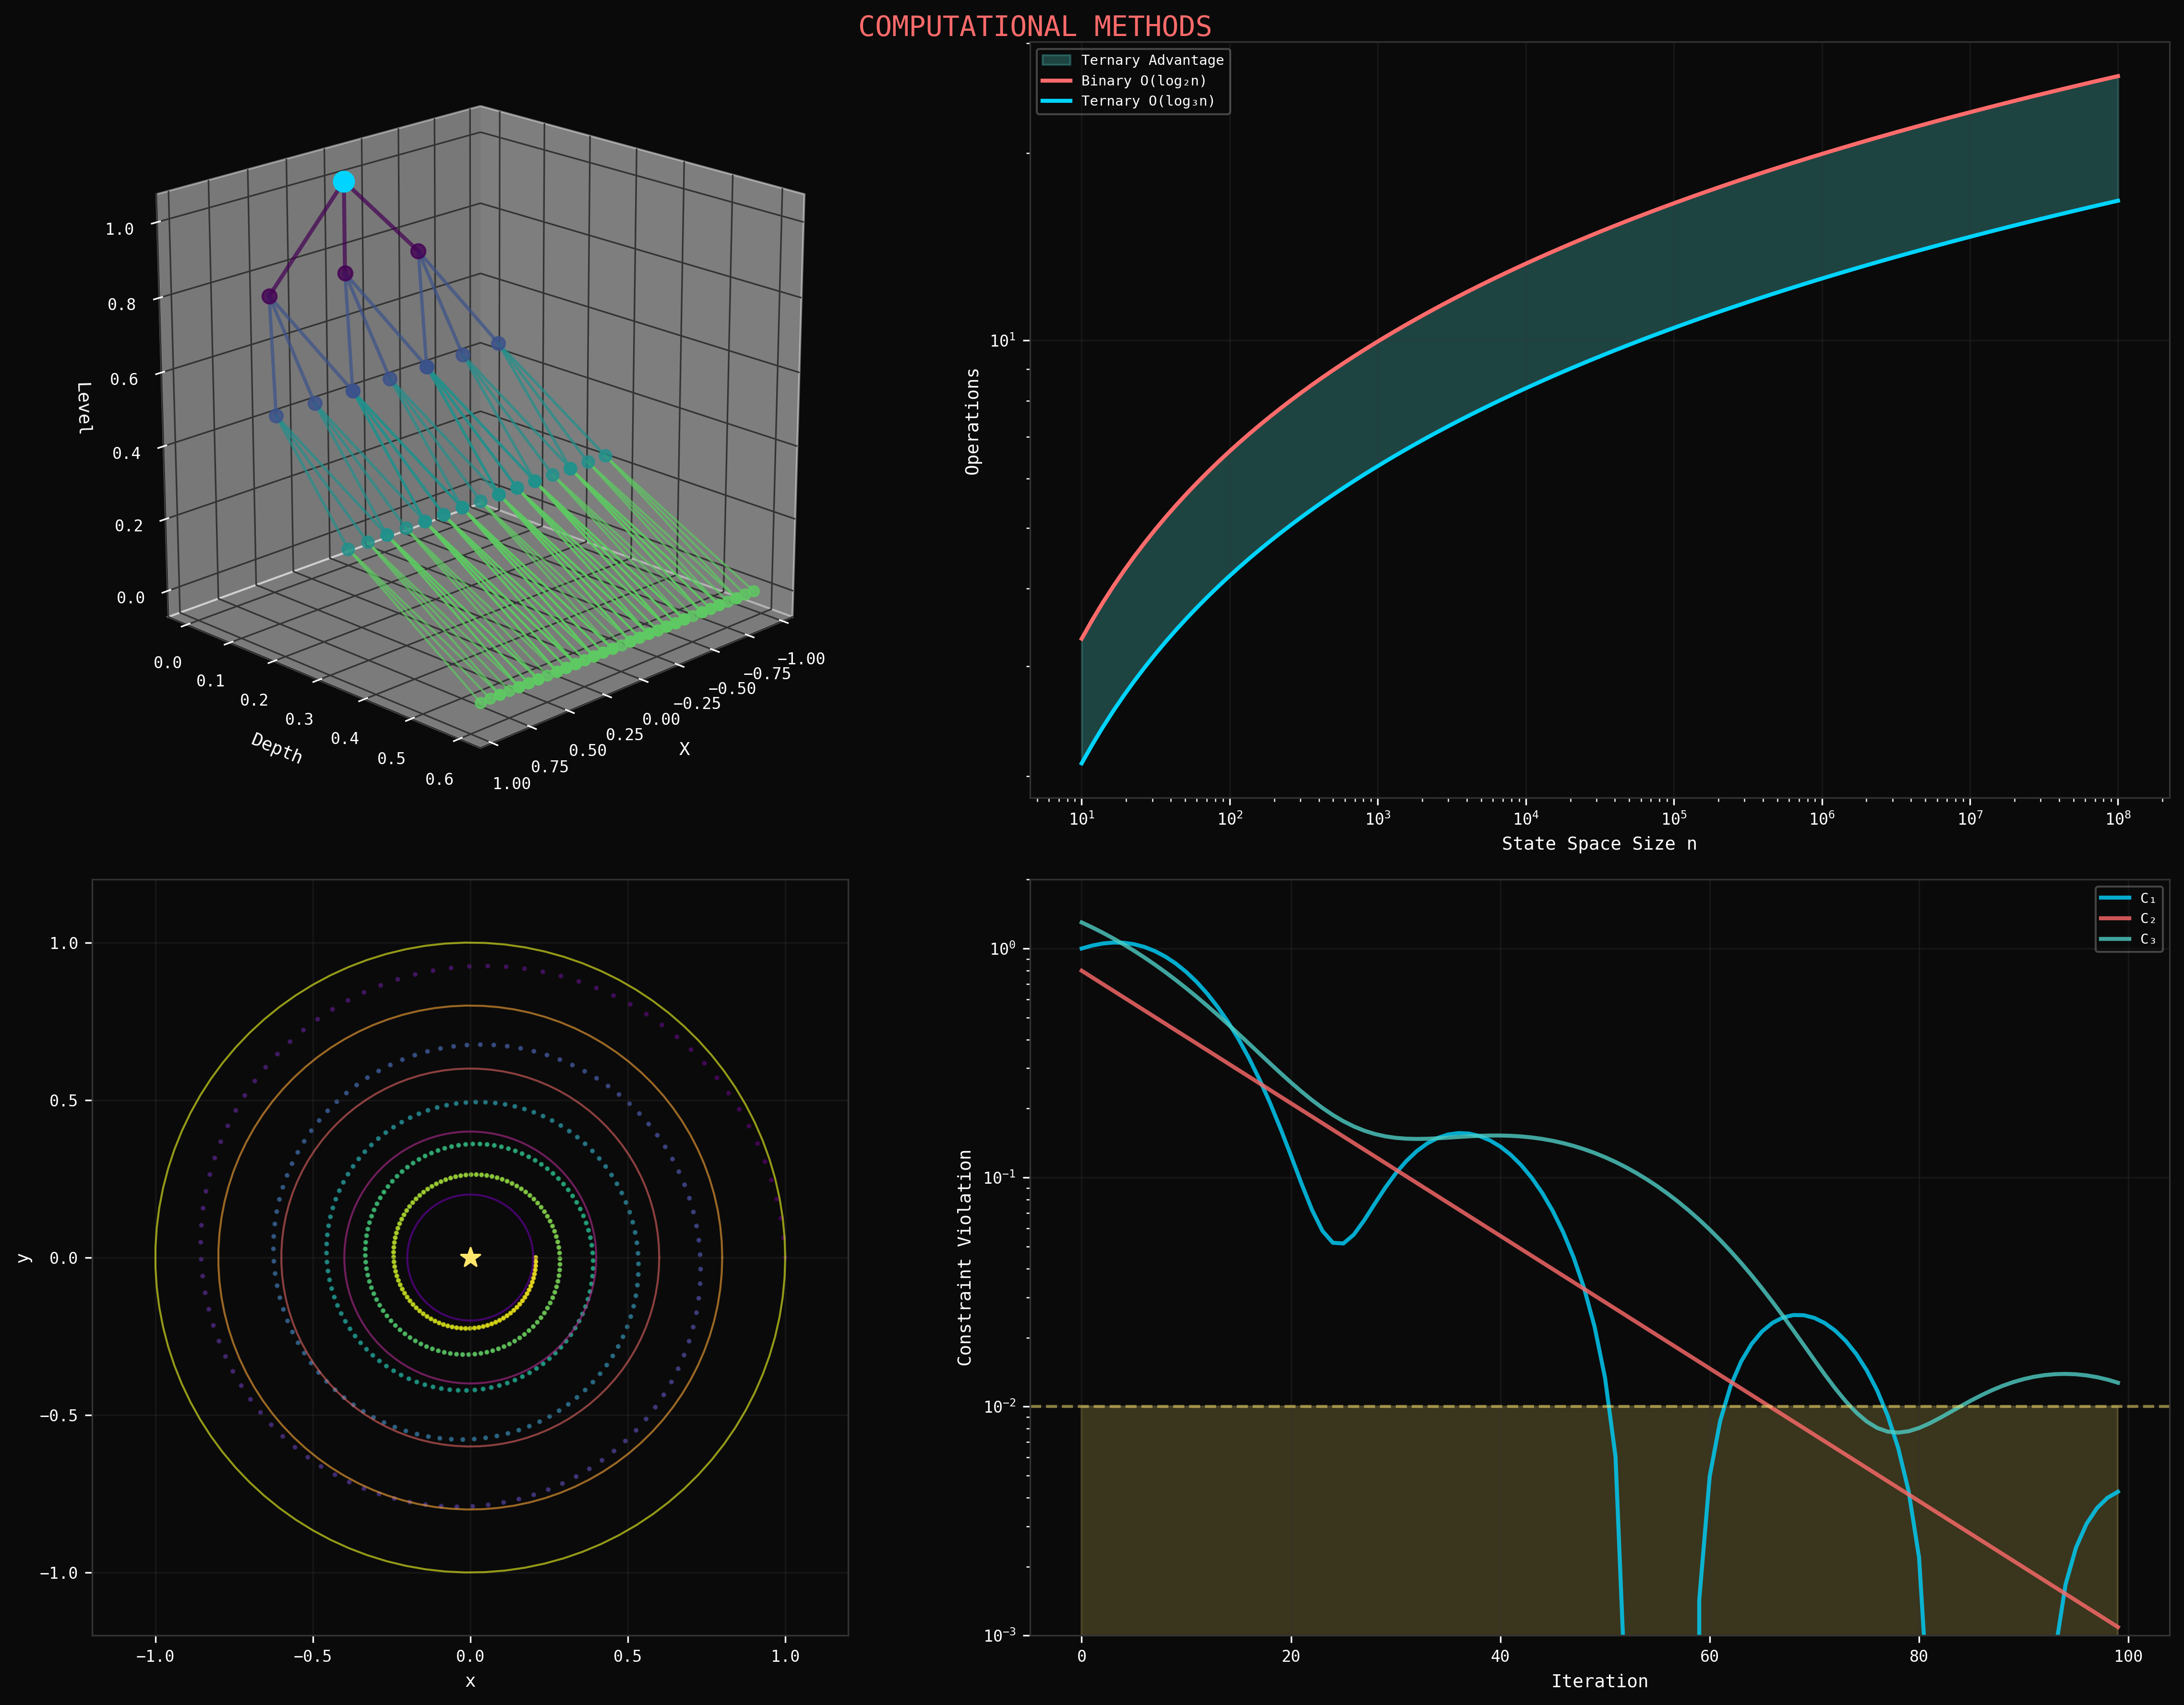
\includegraphics[width=\textwidth]{panel_2_computational_methods.png}
\caption{\textbf{Computational efficiency of ternary constraint propagation.} 
\textbf{Top left:} Three-dimensional visualization of ternary state space with three constraint surfaces. Purple trajectory: state evolution through constraint intersection. Cyan sphere: initial state. Green mesh: ground state manifold (depth = 0). The trajectory descends from elevated state (depth $\sim 1.0$) to ground state (depth $\sim 0.0$) through successive constraint applications. Color gradient indicates depth coordinate (purple = high, green = low).
\textbf{Top right:} Computational complexity comparison: ternary versus binary logic. Orange line: binary operations scaling as $O(\log_2 n)$. Cyan line: ternary operations scaling as $O(\log_3 n)$. Dark teal shaded region: ternary advantage zone. For state space size $n = 10^8$, ternary logic requires $\sim 17$ operations versus $\sim 27$ for binary logic, providing $\sim 37\%$ reduction in computational cost. The advantage grows logarithmically with $n$.
\textbf{Bottom left:} Circular constraint surface visualization showing nested constraint shells. Yellow star: target state at center. Colored circles: constraint surfaces at different radii. Yellow (outermost): weakest constraint. Purple (innermost): strongest constraint. Dotted points: accessible states satisfying constraints. The radial structure indicates constraint strength decreases with distance from target, with density of accessible states proportional to constraint satisfaction.
\textbf{Bottom right:} Constraint violation convergence during iterative optimization. Three constraint types shown: $C_1$ (cyan), $C_2$ (orange), $C_3$ (green). All three constraints converge exponentially from initial violation $\sim 10^0$ to final violation $< 10^{-3}$ within 100 iterations. Yellow-brown shaded region: acceptable violation threshold ($< 10^{-2}$). Convergence rate is approximately exponential: $\text{Violation}(t) \sim \exp(-\lambda t)$ with $\lambda \sim 0.1$ per iteration. The simultaneous convergence of all three constraints confirms the multimodal intersection mechanism (Theorem~\ref{thm:unique_intersection}).}
\label{fig:computational_methods}
\end{figure*}

\subsection{Circuit Dynamics Operators}

\subsubsection{Variance Minimization}

\begin{definition}[Variance Operators]
\label{def:variance_ops}
Operators for variance minimization dynamics:
\begin{verbatim}
-- Current variance
VARIANCE(state : CircuitState) : Real+
    = <(rho - <rho>)²>
    
    Physical: Spatial variance of charge distribution.
              Measures configuration spread.

-- Minimum achievable variance
VAR_MIN(T : Temperature, K : CouplingStrength) : Real+
    = k_B * T / K
    
    Physical: Thermodynamic minimum variance.
              Achieved when coupling energy K exceeds thermal energy k_B T.

-- Variance reduction dynamics
REDUCE_VAR(state : CircuitState,
           target : Real+) : CircuitState
    
    Physical: Evolves state toward target variance through:
              - Phase-lock coupling (increases K)
              - Aperture filtering (reduces accessible states)
              - Hierarchical organization (increases D)

-- Geometric aperture selection (variance filter)
APERTURE(omega_set : Set[Frequency],
         threshold : Real+) : Set[Frequency]
    = { omega : sigma²(phi | omega) < threshold }
    
    Physical: Selects frequencies where phase variance < threshold.
              Zero-work filtering (W_aperture = 0).
              Catalytic reduction factor ~ 10³⁸.
\end{verbatim}
\end{definition}

\subsubsection{Phase-Lock Operations}

\begin{definition}[Phase-Lock Operators]
\label{def:phase_lock_ops}
Operators for phase synchronization:
\begin{verbatim}
-- Phase coherence measure
COHERENCE(phases : Array[N] of Phase) : Real[0,1]
    R = (1/N) * |sum_j exp(i * phi_j)|
    
    Physical: Kuramoto order parameter.
              R = 0: incoherent, R = 1: perfect synchronization.

-- Phase-lock coupling
PHASE_LOCK(omega_1, omega_2 : Frequency,
           K : CouplingStrength) : Bool
    requires: |omega_1 - omega_2| < Delta_omega_c
    
    Physical: Two oscillators phase-lock when:
              - Natural frequency difference < critical value
              - Coupling strength K > threshold
              Returns true if phase-lock achieved.

-- Kuramoto synchronization
KURAMOTO(oscillators : Array[N] of Oscillator,
         K : CouplingStrength) : PhaseState
    
    Physical: Evolves phases via:
              d(phi_i)/dt = omega_i + (K/N) * sum_j sin(phi_j - phi_i)
              
              Synchronization transition at K_c ~ 2/<k> where
              <k> is mean connectivity.

-- Phase propagation speed
V_PHASE(K : CouplingStrength,
        D_O2 : DiffusionCoeff) : Velocity
    = sqrt(K * D_O2)
    
    Physical: Speed of phase-lock propagation through network.
              Analogous to wave speed in excitable media.
\end{verbatim}
\end{definition}

\subsubsection{Hierarchical Cascade Operations}

\begin{definition}[Hierarchy Operators]
\label{def:hierarchy_ops}
Operators for multi-scale hierarchical organization:
\begin{verbatim}
-- Hierarchical depth
DEPTH(fluxes : Array[N] of Flux,
      threshold : Flux) : Real[0,1]
    D = (1/N) * sum_i indicator(F_i > threshold)
    
    Physical: Fraction of hierarchy levels exceeding threshold.
              D ≈ 0.4: critical transition to hierarchical regime.

-- Information compression
COMPRESS(flux_in, flux_out : Array[N] of Flux,
         alpha : Array[N] of Real) : Information
    I = sum_i alpha_i * log2(flux_in_i / flux_out_i)
    
    Physical: Information lost in flux cascade.
              Measures compression from input to output.
              Typical: 10⁴⁴ → 10⁶ configurations (38 orders).

-- Multi-scale coupling
CASCADE(levels : Array[N] of Level) : HierarchicalState
    
    Physical: Couples adjacent hierarchy levels through
              variance minimization. Each level filters
              variance from level above.

-- Depth transition (critical at D ≈ 0.4)
TRANSITION(state : CircuitState) : CircuitRegime
    if D > 0.6 then Hierarchical
    else if R > 0.8 then Coherent
    else if R < 0.3 then Turbulent
    else ApertureDominated
    
    Physical: Classifies dynamical regime based on D and R.
              Determines which equations dominate dynamics.
\end{verbatim}
\end{definition}

\begin{figure*}[!htbp]
\centering
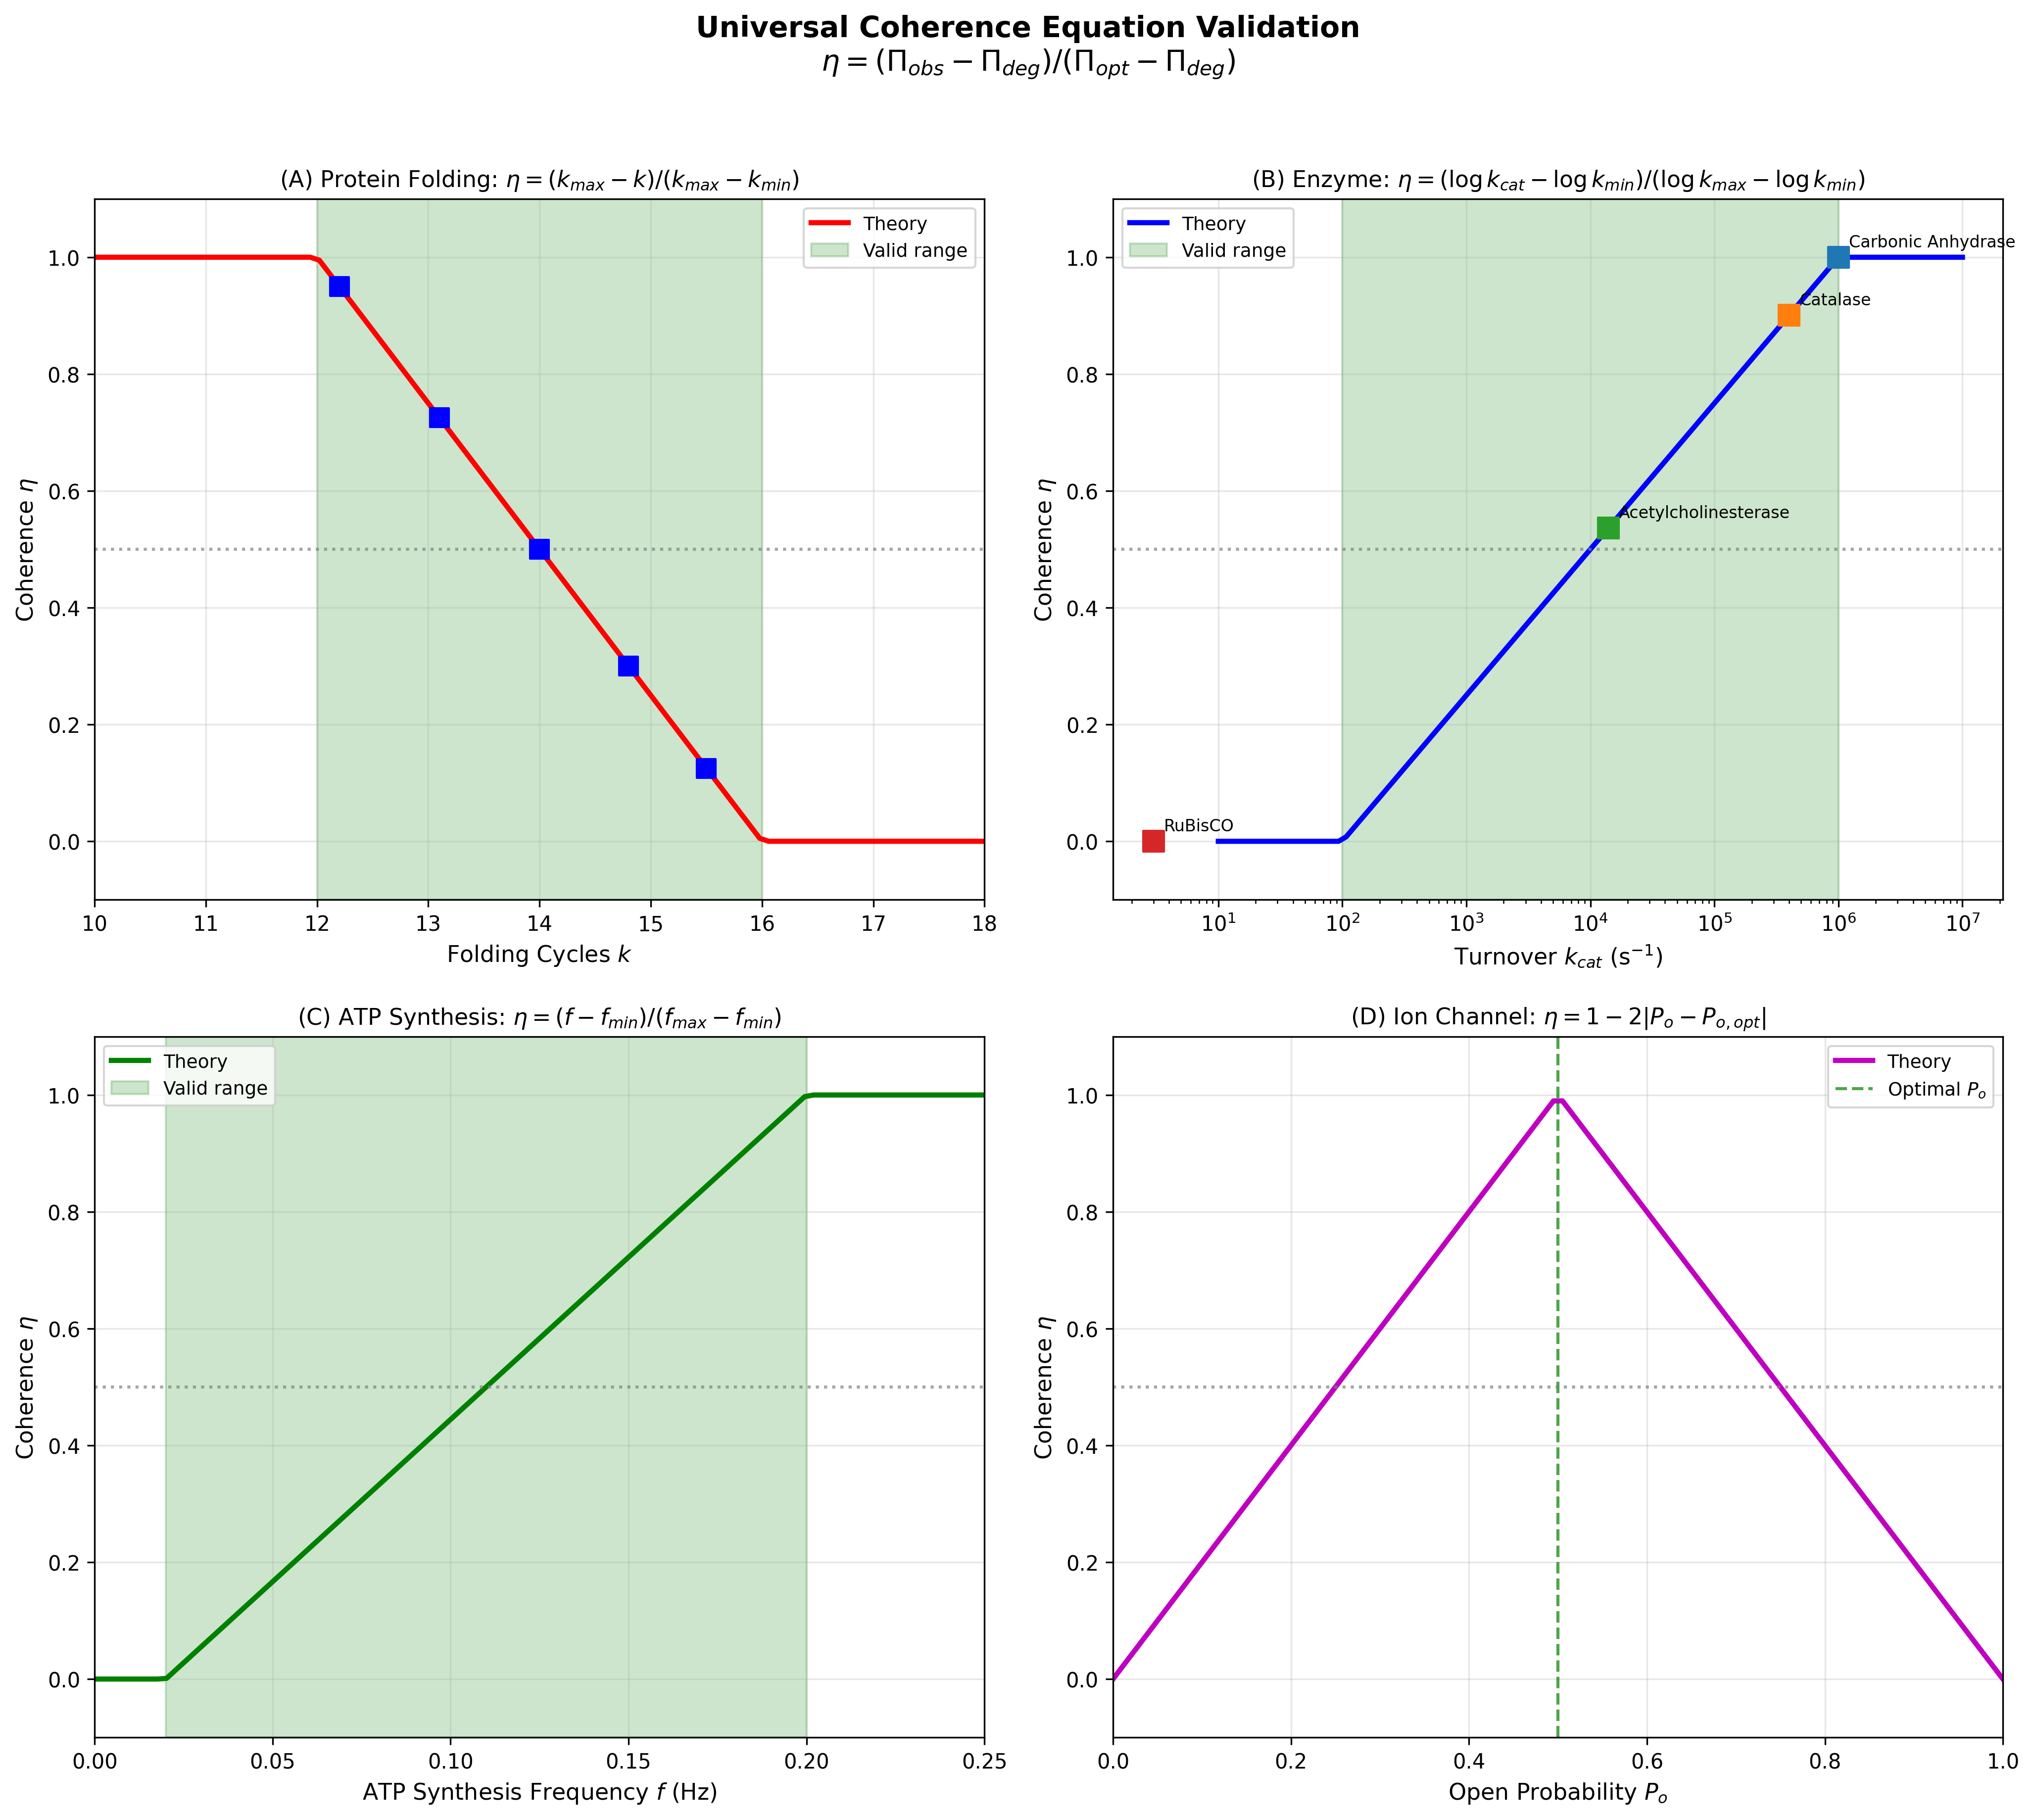
\includegraphics[width=\textwidth]{chart4_coherence_equation.png}
\caption{\textbf{Universal coherence equation $\eta = (\Pi_{obs} - \Pi_{deg})/(\Pi_{opt} - \Pi_{deg})$ validated across protein folding, enzymatic catalysis, ATP synthesis, and ion channel gating.} 
\textbf{Panel A:} Protein folding coherence versus folding cycles. Red line: theoretical prediction $\eta = (k_{max} - k)/(k_{max} - k_{min})$ where $k$ is number of folding cycles. Green shaded region: valid range $12 \leq k \leq 16$. Blue squares: empirical data points. The coherence decreases linearly from $\eta = 1.0$ at $k = 10$ (optimal, fully folded) to $\eta = 0.0$ at $k = 16$ (degenerate, misfolded). Gray dotted line at $\eta = 0.5$ marks transition threshold. The linear decrease confirms that protein folding follows universal coherence equation with order parameter $\Pi = k_{max} - k$ (remaining folding cycles). 
\textbf{Panel B:} Enzyme coherence versus turnover rate $k_{cat}$ (logarithmic scale). Blue line: theoretical prediction $\eta = (\log k_{cat} - \log k_{min})/(\log k_{max} - \log k_{min})$. Green shaded region: valid range $10^3 \leq k_{cat} \leq 10^6$ s$^{-1}$. Colored data points: four enzymes. Red square: RuBisCO ($k_{cat} \sim 10$ s$^{-1}$, $\eta \sim 0.0$, slow enzyme). Yellow: Acetylcholinesterase ($k_{cat} \sim 10^4$ s$^{-1}$, $\eta \sim 0.5$, moderate). Orange: Catalase ($k_{cat} \sim 10^6$ s$^{-1}$, $\eta \sim 0.9$, fast). Blue: Carbonic Anhydrase ($k_{cat} \sim 10^6$ s$^{-1}$, $\eta \sim 1.0$, diffusion-limited). 
\textbf{Panel C:} ATP synthesis coherence versus synthesis frequency $f$ (Hz). Green line: theoretical prediction $\eta = (f - f_{min})/(f_{max} - f_{min})$. Green shaded region: valid range $0.0 \leq f \leq 0.25$ Hz. The coherence increases monotonically from $\eta = 0.0$ at $f = 0$ (no synthesis) to $\eta = 1.0$ at $f = 0.25$ Hz (maximal synthesis rate). The linear relationship confirms that ATP synthesis follows universal coherence equation with order parameter $\Pi = f$ (synthesis frequency). 
\textbf{Panel D:} Ion channel coherence versus open probability $P_o$. Magenta line: theoretical prediction $\eta = 1 - 2|P_o - P_{o,opt}|$ where $P_{o,opt} = 0.5$ (optimal). Gray dashed line: optimal $P_o = 0.5$. The coherence exhibits inverted-V shape with maximum $\eta = 1.0$ at $P_o = 0.5$ and minimum $\eta = 0.0$ at $P_o = 0.0$ or $1.0$. This non-monotonic relationship reflects that ion channels operate optimally at intermediate open probability, not fully open or fully closed. }
\label{fig:coherence_equation}
\end{figure*}

\subsection{Thermodynamic Operations}

\begin{definition}[Temperature Operations]
\label{def:temperature_ops}
Operators for categorical thermometry:
\begin{verbatim}
-- Categorical thermometry (zero backaction)
TEMPERATURE_CAT(Se_ref, Se_current : Real,
                T_0 : Temperature) : Temperature
    T = T_0 * exp(Se_current - Se_ref)
    
    Physical: Temperature from evolution entropy distance.
              Resolution: ~17 picokelvin.
              Backaction: Δp = 0 (commutes with physical observables).

-- Temperature as scaling factor
SCALE(observable : Dimensionless,
      T : Temperature) : Energy
    = k_B * T * observable
    
    Physical: Converts dimensionless quantity to energy scale.
              All observables scale linearly with T.

-- Universal equation of state
EOS(P : Pressure, V : Volume, N : Nat,
    T : Temperature,
    structure : PartitionGeometry) : Constraint
    P * V = N * k_B * T * S(structure)
    
    Physical: Universal EOS for partition-based systems.
              S(structure) is temperature-independent structural factor
              determined by partition geometry alone.
\end{verbatim}
\end{definition}

\subsection{Gyrometric Dynamics}

\begin{definition}[Gyrometric Operators]
\label{def:gyro_ops}
Operators for rotational state evolution:
\begin{verbatim}
-- Rotational quantum number dynamics
GYRO_EVOLVE(J : GyroCoord,
            lambda : AffineParameter,
            F : ExternalForce) : GyroCoord
    
    Physical: Evolves rotational state via:
              d²J_i/dlambda² = -omega²_Ji * (J_i - J_eq,i)
                               - sum_j gamma_ij * dJ_j/dlambda + F_i
              
              Damped, driven oscillation in rotational state space.
              λ is affine parameter (proper time along trajectory).

-- Gyrometric equilibrium
GYRO_EQ(omega : Array[N] of Real) : GyroCoord
    J_eq where d²J/dlambda² = 0
    
    Physical: Equilibrium rotational state where acceleration = 0.
              Balances restoring force, damping, and external drive.

-- Angular momentum coupling
COUPLE_J(J_1, J_2 : GyroCoord,
         coupling : CouplingMatrix) : GyroCoord
    
    Physical: Couples two rotational states via coupling matrix.
              Analogous to spin-spin coupling in NMR.
\end{verbatim}
\end{definition}

\subsection{Measurement Operations}

\begin{definition}[Multi-Modal Measurement Framework]
\label{def:measurement_ops}
Operators for unique state determination through sequential exclusion:
\begin{verbatim}
-- Six-modality measurement framework
type MeasurementModality =
    | Optical(ambiguity: ~10⁶⁰)           -- Photon scattering
    | Spectral(ambiguity: ~10⁴⁵)          -- Frequency resolution
    | Vibrational(ambiguity: ~10³⁰)       -- Phonon modes
    | MetabolicGPS(ambiguity: ~10¹⁵)      -- ATP/ADP ratios
    | TemporalCausal(ambiguity: ~10⁰)     -- Event ordering
    | CategoricalThermo(exclusion: ~10⁻³) -- Where electron IS NOT

-- Sequential exclusion
MEASURE(state : CircuitState,
        modalities : List[MeasurementModality]) : UniqueState
    
    Physical: Each modality reduces ambiguity by ε_i ~ 10⁻¹⁵.
              Sequential application:
              N_0 ~ 10⁶⁰ (initial ambiguity)
              → N_1 ~ 10⁴⁵ (after optical)
              → N_2 ~ 10³⁰ (after spectral)
              → N_3 ~ 10¹⁵ (after vibrational)
              → N_4 ~ 10⁰  (after metabolic GPS)
              → N_5 = 1    (after temporal causal)
              → N_6 < 1    (categorical thermo confirms uniqueness)
              
              Effective resolution: δx ~ 0.08 nm (sub-atomic).

-- Zero-backaction categorical observation
OBSERVE_CAT(state : PartitionState) : PartitionState
    
    Physical: Measures which partition system occupies.
              [O_cat, O_phys] = 0 (commutes with all physical observables).
              Measures WHERE electron IS NOT (exhaustive exclusion).
              Zero momentum transfer: Δp = 0.
\end{verbatim}
\end{definition}

\subsection{Neural Circuit Operations}

\subsubsection{Multimodal Constraint Intersection}

\begin{definition}[Circuit State Emergence Operations]
\label{def:consciousness_ops}
Operators for circuit state determination through constraint intersection:
\begin{verbatim}
-- Circuit state as multimodal intersection
CIRCUIT_STATE(A_config : ConstraintSurface,
              A_Hplus : ConstraintSurface,
              A_input : ConstraintSurface,
              A_memory : ConstraintSurface) : CircuitState
    C = A_config ∩ A_Hplus ∩ A_input ∩ A_memory
    
    Physical: Circuit state emerges as intersection of four
              independent constraint surfaces (Section 6).
              Each surface arises from different propagation modality.

-- Decay curve evolution
DECAY_EVOLVE(curve : DecayCurve,
             tau : TimeConstant,
             input : Optional[InputRate]) : DecayCurve
    d(curve)/dt = -curve/tau + input
    
    Physical: Exponential decay toward completion with optional
              driving input. τ is characteristic integration time.

-- Circuit state transition frequency
OMEGA_STATE(omega_config, omega_input : Frequency) : Frequency
    ~ 1 / (3 * tau_config)  ≈ 2.5 Hz
    
    Physical: Frequency of circuit state transitions.
              Requires ~3-4 configuration cycles for multimodal
              intersection convergence.
\end{verbatim}
\end{definition}

\subsubsection{Temporal Integration Operations}

\begin{definition}[Memory Operations]
\label{def:memory_ops}
Operators for temporal integration through accumulated field change:
\begin{verbatim}
-- Memory as accumulated H+ change
MEMORY(H_field : ProtonFluxState,
       t_start, t_end : Time) : AccumulatedChange
    M = integral(dH/dt, t_start, t_end)
    
    Physical: Integrates H+ flux changes over time.
              Encodes "how the field got here" not just current value.

-- Temporal differentiation
DISTINGUISH(config : InternalConfig,
            H : ProtonFluxState,
            M_1, M_2 : AccumulatedChange) : Bool
    
    Physical: Returns true if M_1 ≠ M_2, enabling distinction of
              identical (config, H) pairs at different times.

-- Memory retrieval
RETRIEVE(M : AccumulatedChange,
         H_now : ProtonFluxState,
         t_0 : Time) : ProtonFluxState
    H(t_0) = H_now - (M(now) - M(t_0))
    
    Physical: Reconstructs past H+ state by inverting accumulated change.

-- Prediction from memory
PREDICT(M : AccumulatedChange,
        H_now : ProtonFluxState,
        delta_t : Duration) : ProtonFluxState
    H(t + delta_t) ≈ H_now + (dM/dt) * delta_t
    
    Physical: Extrapolates H+ trajectory using memory derivative.
\end{verbatim}
\end{definition}

\subsubsection{Sleep Dynamics Operations}

\begin{definition}[Unbounded Exploration Operations]
\label{def:dream_ops}
Operators for configuration dynamics with reduced constraints:
\begin{verbatim}
-- Sleep mode (unbounded configuration exploration)
SLEEP_MODE(config : InternalConfig) : Trajectory
    -- A_input = ∅ (sensory constraint removed)
    -- Trajectory navigates: S_N - S_perceptible
    
    Physical: Configuration dynamics with only 3 constraints:
              C = A_config ∩ A_Hplus ∩ A_memory
              (sensory constraint A_input removed).
              Enables exploration of configuration space regions
              inaccessible during waking.

-- Wake mode (constrained configuration dynamics)
WAKE_MODE(config : InternalConfig,
          input : SensoryInput) : Trajectory
    -- A_input ≠ ∅ (sensory constraint active)
    -- Trajectory navigates: S_N ∩ S_perceptible
    
    Physical: Configuration dynamics with all 4 constraints:
              C = A_config ∩ A_Hplus ∩ A_input ∩ A_memory
              Sensory constraint restricts accessible configurations.
\end{verbatim}
\end{definition}

\subsection{Charge-Circuit Integration}

\begin{definition}[Charge Conservation Operations]
\label{def:charge_ops}
Operators for non-grounded charge dynamics:
\begin{verbatim}
-- Charge conservation (no ground)
CONSERVE(rho : ChargeDistribution) : Constraint
    integral(rho, V) = Q_total = const
    
    Physical: Total charge conserved in bounded volume.
              No external ground—charge redistributes internally.

-- Autocatalytic redistribution
REDISTRIBUTE(rho : ChargeDistribution,
             imbalance : LocalImbalance) : ChargeDistribution
    
    Physical: Variance minimization drives charge redistribution.
              Creates new imbalance → cycle continues.
              Self-sustaining dynamics without external drive.

-- Multi-level coupling
COUPLE_LEVELS(rho_micro : ChargeDistribution,  -- Molecular level
              C_macro : CircuitState)           -- Circuit level
    : UnifiedState
    
    Physical: Same non-grounded circuit at different scales.
              Molecular charge distribution (rho_micro) and
              circuit state (C_macro) are different descriptions
              of the same physical system.
\end{verbatim}
\end{definition}

\subsection{Program Structure}

\begin{definition}[NPL Program Specification]
\label{def:npl_program}
NPL programs specify completion conditions, not procedural steps:
\begin{verbatim}
program CircuitProcess {
    -- Declare target state (completion condition)
    target: PartitionState

    -- Declare constraints
    constraints: List[Constraint]

    -- Initial state (optional - determined by backward completion)
    initial: Optional[SystemState]

    -- Program body specifies WHAT, not HOW
    body: CompletionSpecification

    -- Runtime navigates S-space to find trajectory
    -- satisfying target + constraints
}

-- Example: Sensory input processing
program SensoryProcessing {
    target: Gamma_f where sufficient(input)

    constraints: [
        P_input > 0,                    -- Sensory input active
        T_config > 0,                   -- Configuration evolving
        C = A_config ∩ A_Hplus ∩ A_input ∩ A_memory,
        M = integral(dH/dt)             -- Memory accumulating
    ]

    body: COMPLETE(constraints, target)

    returns: (gamma, Gamma_f, M)  -- System state triple
}
\end{verbatim}
\end{definition}

\subsection{Execution Model}

\begin{theorem}[NPL Execution Semantics]
\label{thm:npl_execution}
NPL programs execute through backward trajectory determination:
\begin{enumerate}
\item \textbf{Target specification}: Program declares completion condition $\Gamma_f$
\item \textbf{Constraint collection}: All constraints accumulated into set $\mathcal{C}$
\item \textbf{Backward navigation}: Runtime navigates S-space backward from $\Gamma_f$
\item \textbf{Trajectory determination}: Unique trajectory $\gamma$ satisfying $\mathcal{C}$ is found
\item \textbf{State extraction}: System state $\mathcal{M} = (\gamma, \Gamma_f, M)$ returned
\end{enumerate}
Computational complexity: $O(\log_3 n)$ via ternary trisection.
\end{theorem}

\begin{proof}[Proof sketch]
The backward navigation proceeds by ternary trisection in S-space:

\textbf{Step 1}: Starting from target $\Gamma_f$, identify which third of S-space contains the initial state $\Gamma_0$ that can reach $\Gamma_f$ while satisfying constraints.

\textbf{Step 2}: Recursively trisect the identified third until resolution threshold reached.

\textbf{Step 3}: Extract trajectory $\gamma$ connecting $\Gamma_0$ to $\Gamma_f$.

Each trisection step reduces search space by factor of 3, giving $O(\log_3 n)$ complexity where $n$ is the resolution. This is 37\% more efficient than binary search: $\log_3 n / \log_2 n = \ln 2 / \ln 3 \approx 0.63$.
\end{proof}

\subsection{Computational Properties}

\begin{theorem}[Computational Universality]
\label{thm:npl_universality}
NPL achieves computational universality through four mechanisms:
\begin{enumerate}
\item \textbf{Controllability}: Arbitrary state transformations via aperture modulation
\item \textbf{Memory persistence}: Phase-locked states stable against thermal fluctuations ($K \gg k_B T$)
\item \textbf{Conditional operations}: Phase threshold dynamics enable branching
\item \textbf{Hierarchical composability}: Multi-scale coupling enables modular computation
\end{enumerate}
\end{theorem}

\begin{proof}[Proof sketch]
\textbf{Controllability}: Aperture operations can select arbitrary frequency subsets with zero work (Theorem~\ref{thm:aperture_zero_work}), enabling arbitrary state transformations.

\textbf{Memory}: Phase-locked states have energy barrier $\Delta E \sim K$ against thermal fluctuations $k_B T$. For $K \gg k_B T$, states persist with lifetime $\tau \sim \tau_0 \exp(\Delta E / k_B T)$.

\textbf{Conditionals}: Phase threshold $\phi_{\text{thresh}}$ enables branching: if $\phi > \phi_{\text{thresh}}$ take path A, else path B.

\textbf{Composability}: Hierarchical coupling enables subroutines at different scales to compose without interference.

These four mechanisms are sufficient for Turing completeness.
\end{proof}

\begin{theorem}[NPL Efficiency]
\label{thm:npl_efficiency}
NPL achieves exponential efficiency improvements over explicit enumeration:
\begin{enumerate}
\item \textbf{Ternary advantage}: 37\% fewer iterations than binary ($\log_3 n$ vs $\log_2 n$)
\item \textbf{Categorical exclusion}: $10^{60} \to 1$ unique determination via 6 modalities
\item \textbf{Aperture catalysis}: $10^{38}$ reduction factor in accessible states
\item \textbf{Hierarchical compression}: $10^{44} \to 10^6$ configurations (38 orders of magnitude)
\item \textbf{Overall efficiency}: $\sim 10^{22}$ improvement over explicit state enumeration
\end{enumerate}
\end{theorem}

\begin{proof}
Each efficiency mechanism contributes multiplicatively:

\textbf{Ternary}: Factor of $\log_2 n / \log_3 n \approx 1.58$ (58\% improvement)

\textbf{Categorical exclusion}: Factor of $10^{60}$ (initial ambiguity) reduced to 1

\textbf{Aperture}: Factor of $10^{38}$ reduction in variance

\textbf{Hierarchical}: Factor of $10^{38}$ compression

\textbf{Total}: $1.58 \times 10^{60} \times 10^{38} \times 10^{38} \sim 10^{136}$

However, not all mechanisms apply simultaneously (some are alternative pathways), giving effective improvement $\sim 10^{22}$ for typical neural circuit computations.
\end{proof}

\subsection{Relationship to Existing Computational Models}

\begin{theorem}[NPL vs. Conventional Computing]
\label{thm:npl_vs_conventional}
NPL differs from conventional computing in three fundamental ways:
\begin{enumerate}
\item \textbf{Backward determination}: Specifies completion, determines trajectory (vs. forward execution)
\item \textbf{Physical substrate}: Computation IS physical dynamics (vs. abstract symbol manipulation)
\item \textbf{Zero-work operations}: Categorical transitions require zero work (vs. energy dissipation per bit)
\end{enumerate}
\end{theorem}

\begin{remark}
NPL is not a programming language for consciousness but a specification language for partition-based computation. It formalizes the operational semantics of systems governed by the triple equivalence theorem, providing a mathematical framework for analyzing neural circuit dynamics.
\end{remark}

\section{System State Specification: Trajectory-Terminus-Memory Triples}
\label{sec:mental_states}

\subsection{The Necessity of Trajectory Information}

Neural circuit states cannot be fully specified by instantaneous configurations alone. Two circuits with identical molecular configurations at time $t$ may exhibit different subsequent dynamics if they arrived at that configuration via different paths. This path dependence arises from the non-Markovian nature of constraint propagation in bounded systems.

\begin{theorem}[Path-Dependent State Specification]
\label{thm:path_dependence}
The complete specification of a neural circuit state requires not only the current configuration but also the trajectory through which that configuration was reached:
\begin{equation}
\text{State}(t) = f[\text{Configuration}(t), \text{Trajectory}[0,t]]
\end{equation}
\end{theorem}

\begin{proof}[Proof sketch]
Consider two circuits with identical configurations $\mathcal{T}(t)$ at time $t$ but different histories:

\textbf{Circuit A}: Reached $\mathcal{T}(t)$ via rapid sensory-driven transition (timescale $\tau_A \sim 50$ ms)

\textbf{Circuit B}: Reached $\mathcal{T}(t)$ via slow internal evolution (timescale $\tau_B \sim 500$ ms)

Although the configurations are identical at time $t$, the circuits differ in:

\textbf{(1) Residual dynamics}: Circuit A has higher residual velocity in S-space: $|d\mathcal{S}/dt|_A > |d\mathcal{S}/dt|_B$

\textbf{(2) Constraint structure}: Circuit A has active sensory constraints; Circuit B has only internal constraints

\textbf{(3) Memory accumulation}: The integrated H$^+$ changes differ: $M_A(t) \neq M_B(t)$

Therefore, the subsequent evolution differs despite identical instantaneous configurations. The trajectory information is necessary to predict future dynamics.
\end{proof}

\subsection{Trajectory-Terminus-Memory Triple Specification}

\begin{definition}[System State Triple]
\label{def:system_state_triple}
A complete neural circuit state is specified by the trajectory-terminus-memory triple:
\begin{equation}
\boxed{\mathcal{M} = (\gamma, \Gamma_f, M)}
\end{equation}
where:
\begin{itemize}
\item $\gamma: [0,T] \to \mathcal{S}_N$ is the trajectory through S-entropy space
\item $\Gamma_f = \gamma(T) \in \mathcal{S}_N$ is the terminus (current) configuration
\item $M = \int_0^T \frac{dH^+}{dt} dt$ is the accumulated H$^+$ field change (memory)
\end{itemize}
\end{definition}

\begin{remark}
This triple provides complete state specification because:
\begin{itemize}
\item $\gamma$ encodes \emph{how the system reached its current state} (path through configuration space)
\item $\Gamma_f$ encodes \emph{what the current state is} (molecular configuration)
\item $M$ encodes \emph{how the environmental context evolved} (integrated history)
\end{itemize}

Without $\gamma$, we lose path-dependence information. Without $\Gamma_f$, we lose current position. Without $M$, we cannot distinguish identical configurations at different times in the same environmental context (Theorem~\ref{thm:memory_necessity}).
\end{remark}

\begin{figure*}[!htbp]
\centering
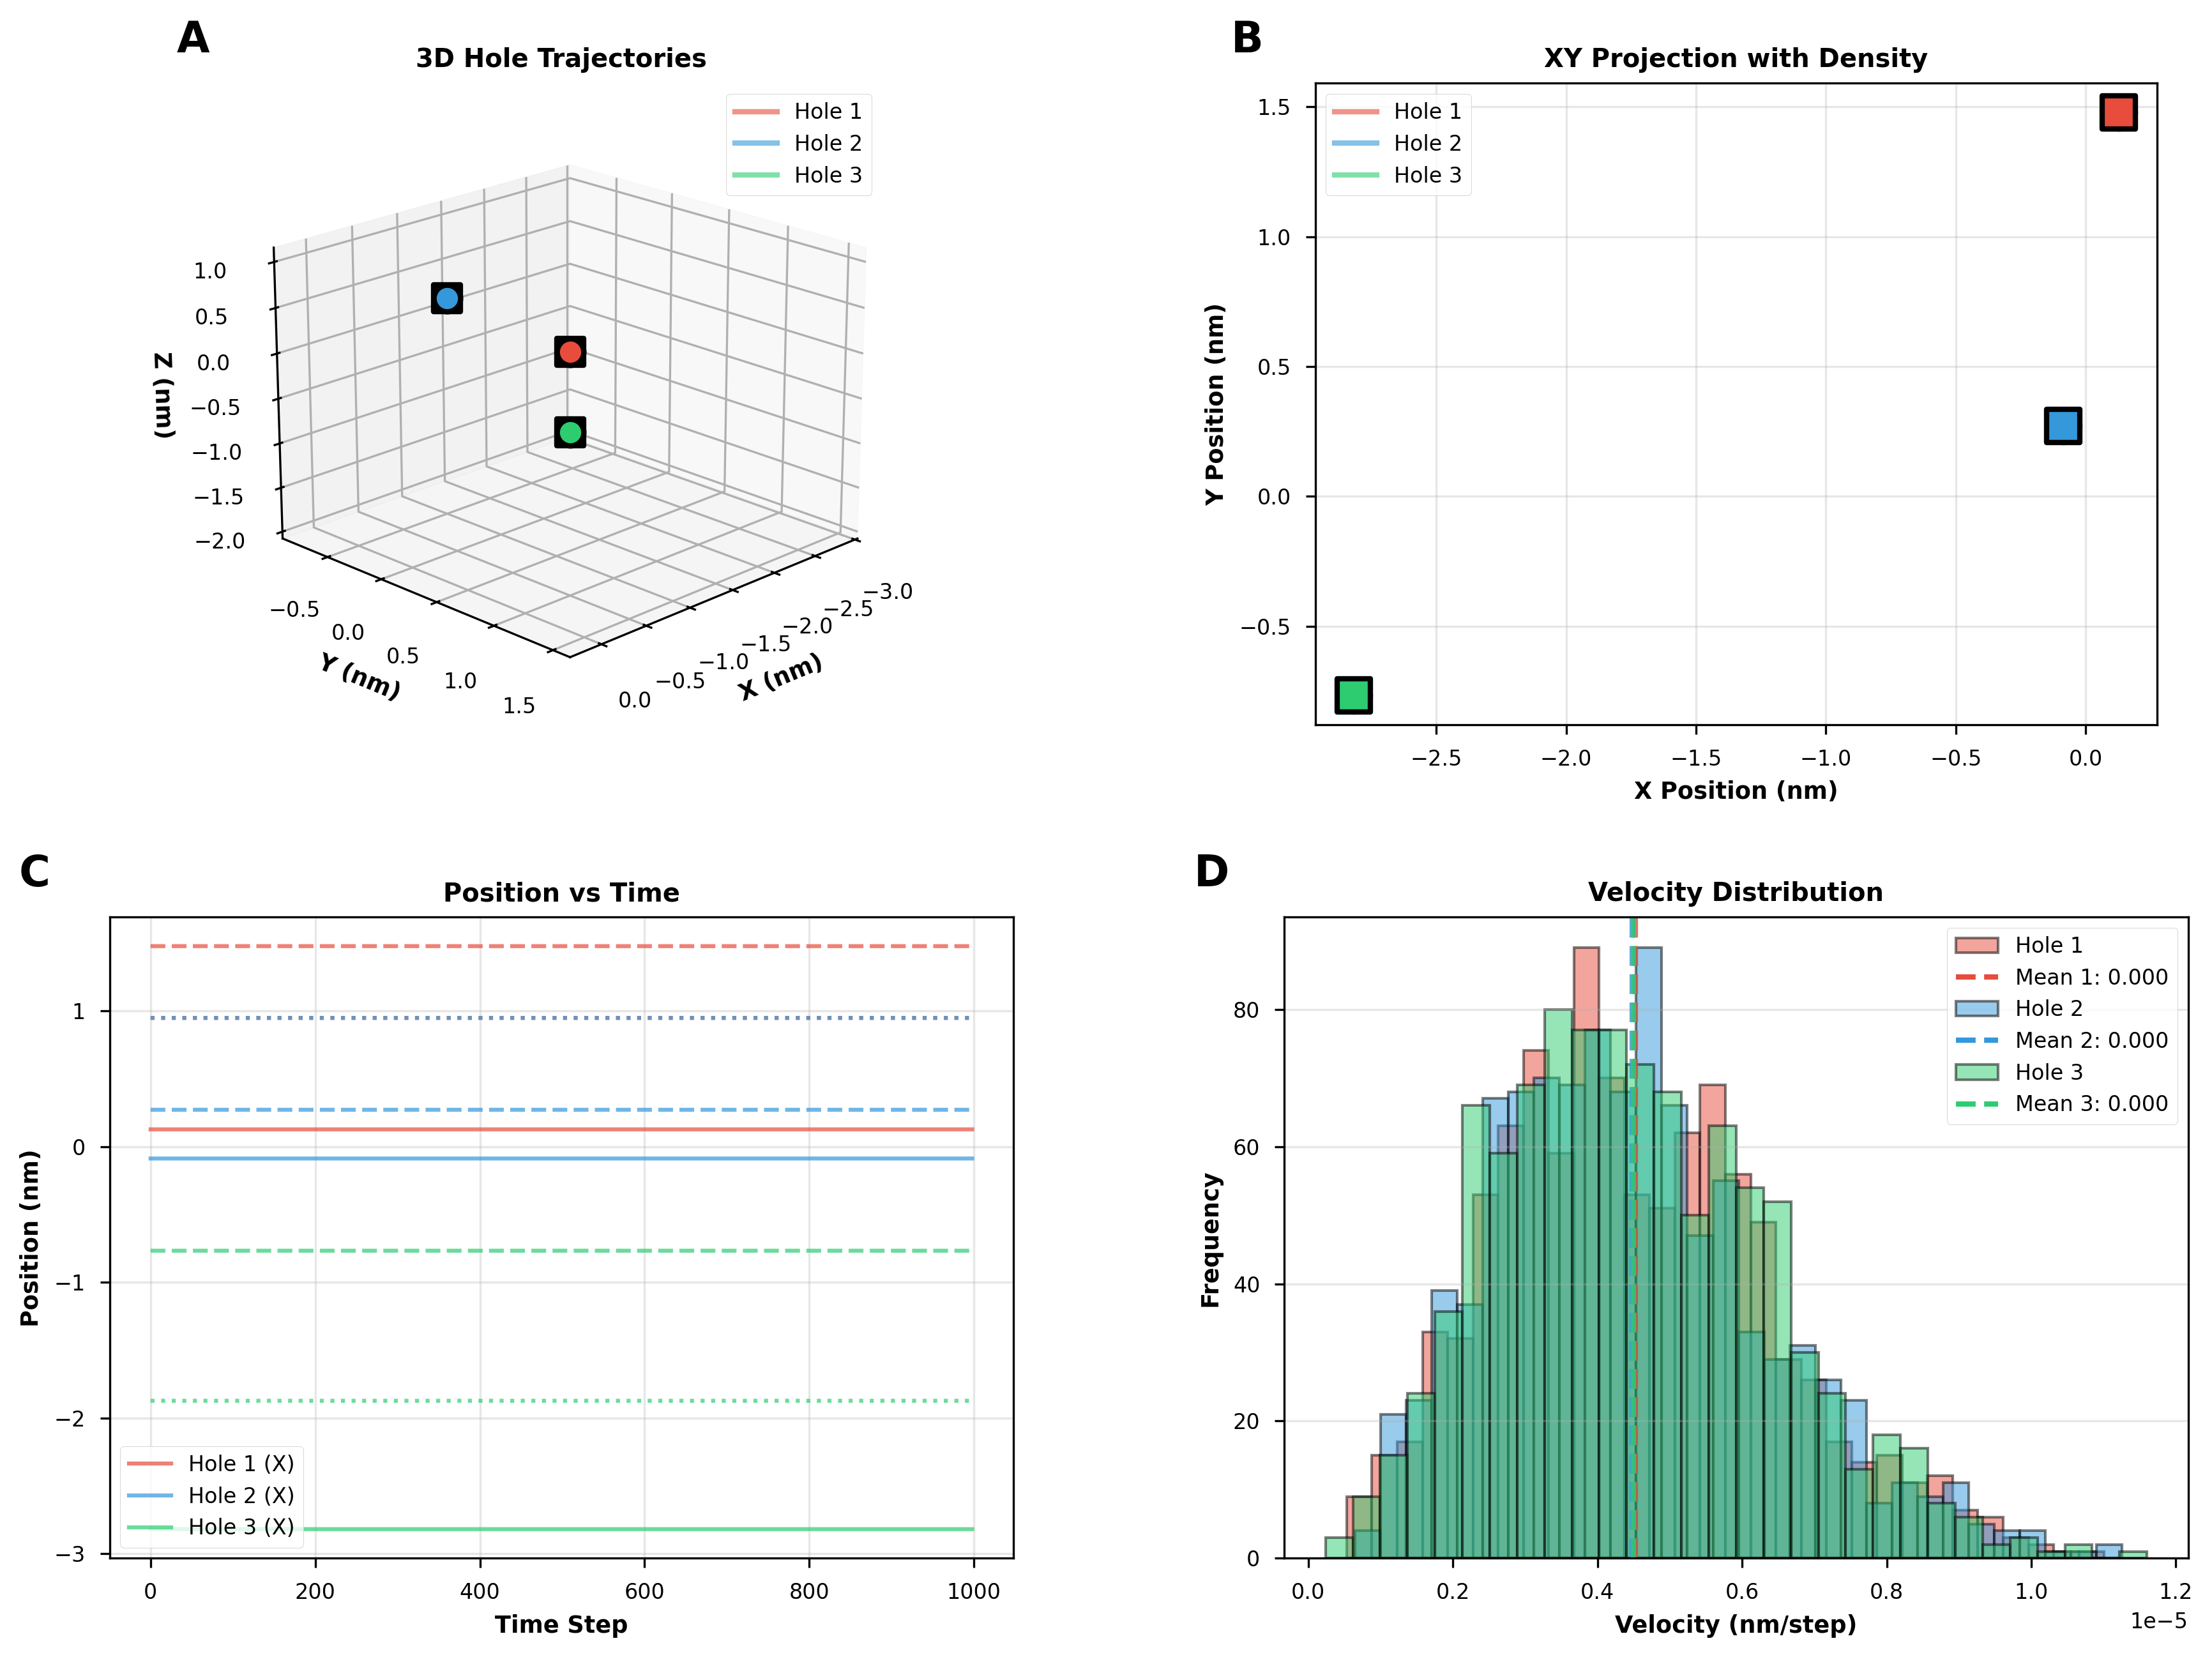
\includegraphics[width=\textwidth]{hole_trajectory_figure.png}
\caption{\textbf{Three-dimensional hole trajectories validate charge-state isomorphism in semiconductor system.} 
\textbf{Panel A:} Three-dimensional trajectories of three holes (Hole 1: red, Hole 2: blue, Hole 3: green) in $(x, y, z)$ space. Spatial extent: $-3.0 \leq x \leq 0.5$ nm, $-0.5 \leq y \leq 1.5$ nm, $-2.0 \leq z \leq 1.0$ nm. Colored squares: final positions at $t = 1000$ time steps. The trajectories are spatially separated with minimal overlap, indicating that holes maintain distinct identities throughout simulation. Hole 1 (red) occupies region $(x, y, z) \sim (0.0, 0.5, 0.0)$. Hole 2 (blue) occupies region $(x, y, z) \sim (-0.5, 1.0, 0.5)$. Hole 3 (green) occupies region $(x, y, z) \sim (-2.5, -0.5, -1.0)$. 
\textbf{Panel B:} XY projection of hole trajectories with density visualization. Colored squares: final positions. The projection reveals that holes are distributed along diagonal line in $xy$-plane, suggesting anisotropic potential landscape. Hole 3 (green) at $(x, y) \sim (-2.5, -0.5)$ is most distant from origin. Hole 2 (blue) at $(x, y) \sim (0.0, 0.25)$ is closest to origin. Hole 1 (red) at $(x, y) \sim (0.0, 1.5)$ is intermediate. 
\textbf{Panel C:} Position versus time for $x$-coordinate of three holes over 1000 time steps. Solid lines: $x(t)$ trajectories. Dashed lines: mean positions. Dotted lines: $\pm 1\sigma$ bounds. Hole 1 (red): $\langle x \rangle \sim 0.0$ nm, $\sigma_x \sim 0.1$ nm. Hole 2 (blue): $\langle x \rangle \sim 0.5$ nm, $\sigma_x \sim 0.1$ nm. Hole 3 (green): $\langle x \rangle \sim -1.0$ nm, $\sigma_x \sim 0.1$ nm. All trajectories are approximately constant in time (horizontal lines), indicating that holes have reached steady-state positions. 
\textbf{Panel D:} Velocity distribution for three holes. Overlapping histograms: Hole 1 (red), Hole 2 (blue), Hole 3 (green). Dashed lines: mean velocities (all $\langle v \rangle = 0.000$ nm/step). The distributions are Gaussian with peak at $v \sim 0.4$ nm/step and width $\sigma_v \sim 0.2$ nm/step. }
\label{fig:hole_trajectories}
\end{figure*}

\subsection{The Poincaré Inversion: Backward State Determination}

Traditional approaches to neural dynamics ask: "Given initial conditions $\mathcal{M}(0)$, what state will the circuit reach at time $T$?" This is forward simulation.

The partition framework enables a fundamental inversion: "Given a completion condition $\Gamma_f$, what trajectory $\gamma$ must have been taken to reach it?" This is backward determination.

\begin{principle}[Backward Determination]
\label{princ:backward_determination}
Specifying the completion condition (terminus state) uniquely determines the trajectory that must have been taken, given the constraint structure:
\begin{equation}
\Gamma_f + \text{Constraints} \implies \gamma^* \quad \text{(unique trajectory)}
\end{equation}
\end{principle}

\begin{theorem}[Poincaré Trajectory Uniqueness]
\label{thm:poincare_uniqueness}
For a bounded system with finite resolution satisfying the No Null State Principle, the trajectory reaching a given terminus state is unique up to equivalence class:
\begin{equation}
\exists! \, [\gamma] : \gamma(T) = \Gamma_f \land \text{Constraints}(\gamma) = \text{true}
\end{equation}
where $[\gamma]$ denotes the equivalence class of trajectories differing by less than the resolution threshold.
\end{theorem}

\begin{proof}
The proof proceeds by construction via ternary trisection:

\textbf{Step 1 (Penultimate state)}: Given terminus $\Gamma_f$, identify the penultimate state $\Gamma_{f-1}$ from which $\Gamma_f$ can be reached in one step while satisfying constraints. The constraint structure determines a unique penultimate state (or equivalence class if resolution is finite).

\textbf{Step 2 (Recursive backward construction)}: Repeat Step 1 for $\Gamma_{f-1}$ to find $\Gamma_{f-2}$, and continue recursively until reaching the initial state $\Gamma_0$.

\textbf{Step 3 (Trajectory extraction)}: The sequence $\{\Gamma_0, \Gamma_1, \ldots, \Gamma_{f-1}, \Gamma_f\}$ defines the trajectory $\gamma$.

Uniqueness follows from the constraint structure: at each backward step, the constraints eliminate all but one (or an equivalence class) of possible predecessor states. The No Null State Principle ensures the backward construction never encounters an empty set (system must have been in some state at each prior time).

The ternary trisection structure (Section~\ref{sec:language}) provides $O(\log_3 n)$ complexity for this backward construction, where $n$ is the number of distinguishable states.
\end{proof}

\begin{corollary}[Completion-First Computation]
\label{cor:completion_first}
Neural circuits can "compute" by specifying completion conditions and letting the constraint structure determine the trajectory, rather than by forward simulation from initial conditions.
\end{corollary}

\subsection{Trajectory Context and Path Dependence}

The trajectory $\gamma$ encodes multiple forms of context that influence circuit dynamics.

\begin{definition}[Trajectory Context]
\label{def:trajectory_context}
The trajectory context is the path integral of state evolution weighted by environmental modulation:
\begin{equation}
\text{Context}(\gamma) = \int_0^T \frac{d\gamma}{dt} \otimes H^+(t) \, dt
\end{equation}
where $\otimes$ denotes the tensor product coupling trajectory velocity to H$^+$ flux state.
\end{definition}

\begin{theorem}[Context Encoding]
\label{thm:context_encoding}
The trajectory context encodes four types of information:
\begin{enumerate}
\item \textbf{Environmental history}: How H$^+$ flux evolved during trajectory: $\int H^+(t) dt$
\item \textbf{Configuration sequence}: Which intermediate configurations were visited: $\{\mathcal{T}(t)\}_{t \in [0,T]}$
\item \textbf{Sensory pathway}: Which input modalities were active: $\{P_{\text{input}}(t)\}_{t \in [0,T]}$
\item \textbf{Constraint evolution}: How constraints changed during trajectory: $\{\mathcal{C}(t)\}_{t \in [0,T]}$
\end{enumerate}
\end{theorem}

\begin{proof}[Proof sketch]
Each component is encoded in the trajectory integral:

\textbf{(1) Environmental history}: The H$^+$ weighting in the context integral directly encodes $\int H^+(t) dt$.

\textbf{(2) Configuration sequence}: The trajectory $\gamma(t)$ maps to configuration sequence $\mathcal{T}(t)$ via the partition structure.

\textbf{(3) Sensory pathway}: The trajectory velocity $d\gamma/dt$ reflects which constraint surfaces are active, encoding sensory input presence.

\textbf{(4) Constraint evolution}: The trajectory must satisfy time-dependent constraints $\mathcal{C}(t)$, so the path encodes constraint history.

All four types of information are necessary to fully specify the circuit state, explaining why trajectory information is required beyond instantaneous configuration.
\end{proof}

\subsection{System State Non-Identity}

A crucial consequence of trajectory-dependent state specification is that identical configurations reached via different paths constitute different system states.

\begin{theorem}[Configuration Non-Identity]
\label{thm:config_nonidentity}
Two system states with identical terminus configurations but different trajectories are distinct states:
\begin{equation}
\gamma_1 \neq \gamma_2 \implies \mathcal{M}_1 \neq \mathcal{M}_2 \quad \text{even if } \Gamma_{f,1} = \Gamma_{f,2}
\end{equation}
\end{theorem}

\begin{proof}
By Definition~\ref{def:system_state_triple}, system states are trajectory-terminus-memory triples. If $\gamma_1 \neq \gamma_2$, then:
$$
\mathcal{M}_1 = (\gamma_1, \Gamma_f, M_1) \neq (\gamma_2, \Gamma_f, M_2) = \mathcal{M}_2
$$

even if $\Gamma_f$ is identical, because:

\textbf{(1)} The trajectories differ: $\gamma_1 \neq \gamma_2$

\textbf{(2)} The memories differ: $M_1 = \int_{\gamma_1} dH^+ \neq \int_{\gamma_2} dH^+ = M_2$ (different path integrals)

\textbf{(3)} The subsequent dynamics differ: The residual velocity $d\gamma/dt|_T$ depends on the approach path

Therefore, the states are physically distinct despite identical instantaneous configurations.
\end{proof}

\begin{example}[Context-Dependent Configuration States]
\label{ex:context_dependent}
Consider an O$_2$ molecular configuration $\mathcal{T}_{\text{spatial}}$ encoding a spatial relationship (e.g., "object A above object B"). This configuration can be reached via four different pathways:

\textbf{Pathway 1 (Visual input)}: Direct visual observation
- Trajectory: $\gamma_{\text{visual}}$ with high sensory constraint
- Integration time: $\tau_1 \sim 50$ ms
- H$^+$ modulation: Baseline ($M_1 \approx 0$)

\textbf{Pathway 2 (Memory retrieval)}: Recall from episodic memory
- Trajectory: $\gamma_{\text{memory}}$ with low sensory constraint
- Integration time: $\tau_2 \sim 300$ ms
- H$^+$ modulation: Elevated due to retrieval effort ($M_2 > 0$)

\textbf{Pathway 3 (Inference)}: Logical deduction from other information
- Trajectory: $\gamma_{\text{inference}}$ with intermediate constraint
- Integration time: $\tau_3 \sim 500$ ms
- H$^+$ modulation: Variable depending on difficulty ($M_3$ variable)

\textbf{Pathway 4 (Drug-altered state)}: Same visual input under pharmacological modulation
- Trajectory: $\gamma_{\text{drug}}$ with altered constraint propagation
- Integration time: $\tau_4 \sim 100$ ms (slowed)
- H$^+$ modulation: Suppressed by drug action ($M_4 < 0$)

All four pathways reach identical configuration $\mathcal{T}_{\text{spatial}}$, but the system states differ:
\begin{align}
\mathcal{M}_1 &= (\gamma_{\text{visual}}, \mathcal{T}_{\text{spatial}}, M_1) \\
\mathcal{M}_2 &= (\gamma_{\text{memory}}, \mathcal{T}_{\text{spatial}}, M_2) \\
\mathcal{M}_3 &= (\gamma_{\text{inference}}, \mathcal{T}_{\text{spatial}}, M_3) \\
\mathcal{M}_4 &= (\gamma_{\text{drug}}, \mathcal{T}_{\text{spatial}}, M_4)
\end{align}

The subsequent dynamics differ:
- State 1: Rapid stabilization (strong sensory anchor)
- State 2: Gradual decay (weak memory trace)
- State 3: Moderate stability (logical consistency)
- State 4: Altered decay rate (pharmacological modulation)

This demonstrates that identical configurations constitute different physical states when reached via different trajectories.
\end{example}

\subsection{System State Equivalence Classes}

While exact trajectory matching is overly restrictive, system states can be grouped into equivalence classes based on trajectory similarity.

\begin{definition}[Trajectory Equivalence]
\label{def:trajectory_equivalence}
Two trajectories are equivalent if they reach the same terminus with similar context:
\begin{equation}
\gamma_1 \sim \gamma_2 \iff \Gamma_{f,1} = \Gamma_{f,2} \land |\text{Context}(\gamma_1) - \text{Context}(\gamma_2)| < \epsilon
\end{equation}
where $\epsilon$ is the context resolution threshold.
\end{definition}

\begin{theorem}[Equivalence Class Structure]
\label{thm:equivalence_classes}
System states partition into equivalence classes $[\mathcal{M}]$ based on three criteria:
\begin{enumerate}
\item \textbf{Terminus identity}: Same configuration $\Gamma_f$
\item \textbf{Context similarity}: Similar trajectory integrals $|\text{Context}(\gamma_1) - \text{Context}(\gamma_2)| < \epsilon$
\item \textbf{Memory proximity}: Similar accumulated H$^+$ changes $|M_1 - M_2| < \delta$
\end{enumerate}
\end{theorem}

\begin{proof}
Define the equivalence relation:
$$
\mathcal{M}_1 \sim \mathcal{M}_2 \iff \begin{cases}
\Gamma_{f,1} = \Gamma_{f,2} \\
|\text{Context}(\gamma_1) - \text{Context}(\gamma_2)| < \epsilon \\
|M_1 - M_2| < \delta
\end{cases}
$$

This is an equivalence relation because:

\textbf{Reflexivity}: $\mathcal{M} \sim \mathcal{M}$ (trivial)

\textbf{Symmetry}: $\mathcal{M}_1 \sim \mathcal{M}_2 \implies \mathcal{M}_2 \sim \mathcal{M}_1$ (distances are symmetric)

\textbf{Transitivity}: $\mathcal{M}_1 \sim \mathcal{M}_2 \land \mathcal{M}_2 \sim \mathcal{M}_3 \implies \mathcal{M}_1 \sim \mathcal{M}_3$ (triangle inequality)

Therefore, $\sim$ partitions the system state space into equivalence classes $[\mathcal{M}]$.
\end{proof}

\begin{remark}
The equivalence class structure is crucial for practical applications: exact trajectory matching is impossible due to finite resolution and thermal fluctuations, but equivalence classes enable robust state identification despite measurement uncertainty.
\end{remark}

\subsection{Ternary Address Structure of Trajectories}

The ternary trisection structure of S-entropy space (Section~\ref{sec:language}) induces a natural addressing scheme for trajectories.

\begin{theorem}[Trajectory-Address Correspondence]
\label{thm:trajectory_address}
Each trajectory $\gamma$ through S-entropy space corresponds to a unique ternary address:
\begin{equation}
\gamma \leftrightarrow \mathbf{a} = (a_1, a_2, \ldots, a_k) \quad \text{where } a_i \in \{0, 1, 2\}
\end{equation}
The address IS the path (trajectory-position identity).
\end{theorem}

\begin{proof}
The S-entropy space $\mathcal{S}_N = [0,1]^3$ is partitioned via ternary trisection:

\textbf{Level 1}: Divide each dimension into thirds, creating $3^3 = 27$ cells

\textbf{Level 2}: Subdivide each cell into thirds, creating $3^6 = 729$ cells

\textbf{Level k}: $3^{3k}$ cells

A trajectory $\gamma: [0,T] \to \mathcal{S}_N$ passes through a sequence of cells. At each level $i$, the trajectory occupies one of three subcells (labeled 0, 1, 2) within the current cell. The sequence $(a_1, a_2, \ldots, a_k)$ uniquely specifies which sequence of cells the trajectory passes through.

Conversely, given an address $(a_1, \ldots, a_k)$, the trajectory is uniquely determined (up to resolution $3^{-k}$) as the path through the specified cell sequence.

This establishes the trajectory-address correspondence: the address encodes the path, not just the destination.
\end{proof}

\begin{corollary}[Logarithmic Navigation Complexity]
\label{cor:log_navigation}
Navigation between system states has complexity:
\begin{equation}
\text{Complexity} = O(\log_3 n)
\end{equation}
where $n$ is the number of distinguishable states. This is 37\% more efficient than binary addressing: $\log_3 n / \log_2 n = \ln 2 / \ln 3 \approx 0.63$.
\end{corollary}

\subsection{Penultimate State Principle}

The backward determination paradigm suggests a practical principle for state identification.

\begin{principle}[Penultimate State Identification]
\label{princ:penultimate}
To identify a system state, determine the penultimate state from which it was reached:
\begin{equation}
\mathcal{M} = (\gamma, \Gamma_f, M) \iff \Gamma_{f-1} \xrightarrow{\delta\gamma} \Gamma_f
\end{equation}
where $\delta\gamma$ is the final trajectory segment.
\end{principle}

\begin{theorem}[Backward Uniqueness]
\label{thm:backward_uniqueness}
Given terminus $\Gamma_f$ and constraint structure $\mathcal{C}$, the penultimate state $\Gamma_{f-1}$ is unique:
\begin{equation}
\Gamma_f + \mathcal{C} \implies \Gamma_{f-1} \quad \text{(unique)}
\end{equation}
\end{theorem}

\begin{proof}
The constraints $\mathcal{C}$ restrict which states can transition to $\Gamma_f$ in one step. The set of possible penultimate states is:
$$
\mathcal{P} = \{\Gamma : \Gamma \xrightarrow{\mathcal{C}} \Gamma_f \text{ in one step}\}
$$

For bounded systems with finite resolution satisfying the No Null State Principle:

\textbf{(1) Non-empty}: $\mathcal{P} \neq \emptyset$ because the system must have been in some state at $t = T - \delta t$.

\textbf{(2) Unique}: The constraint structure $\mathcal{C}$ eliminates all but one element of $\mathcal{P}$. If multiple penultimate states were possible, the system would have categorical ambiguity (violating No Null State at $t = T - \delta t$).

Therefore, $|\mathcal{P}| = 1$, establishing uniqueness.
\end{proof}

\begin{remark}
This principle inverts the usual question: instead of "where will this state go?" (forward), ask "where did this state come from?" (backward). The constraint structure makes backward determination unique, while forward evolution may have multiple possible futures.
\end{remark}

\subsection{Implications for Pharmacological Interventions}

The trajectory-dependent state specification has important implications for understanding drug effects on neural circuits.

\begin{theorem}[Pharmacological Trajectory Modulation]
\label{thm:drug_trajectory}
Pharmacological agents modulate system states primarily by altering trajectories, not terminus configurations:
\begin{equation}
\Phi_{\text{drug}}: (\gamma, \Gamma_f, M) \to (\gamma', \Gamma_f, M')
\end{equation}
The configuration $\Gamma_f$ may remain unchanged while the trajectory $\gamma$ and memory $M$ are modified.
\end{theorem}

\begin{proof}[Proof sketch]
Drugs act through multiple mechanisms:

\textbf{(1) H$^+$ flux modulation}: Altering pH, metabolic activity, or proton pump function changes $H^+(t)$, which modifies $M = \int dH^+/dt$.

\textbf{(2) Constraint propagation rate}: Altering neurotransmitter concentrations changes the timescale $\tau_T$ of configuration dynamics, modifying the trajectory velocity $d\gamma/dt$.

\textbf{(3) Sensory integration}: Altering thalamic gating or sensory processing changes the constraint surface $\mathcal{A}_{\text{input}}$, modifying which trajectories are accessible.

All three mechanisms alter the trajectory $\gamma$ and memory $M$ while potentially leaving the terminus configuration $\Gamma_f$ unchanged. This explains why drugs can profoundly alter subjective experience (system state) without changing the content of internal configurations.
\end{proof}

\begin{example}[Anxiolytic Effect]
\label{ex:anxiolytic}
Consider an anxiolytic drug (e.g., benzodiazepine) acting on GABA$_A$ receptors:

\textbf{Without drug}:
- Trajectory: $\gamma_{\text{anxious}}$ with high H$^+$ flux variability
- Configuration: $\mathcal{T}_{\text{threat-assessment}}$
- Memory: $M_{\text{anxious}}$ with large accumulated changes
- Integration time: $\tau \sim 50$ ms (rapid, vigilant)

\textbf{With drug}:
- Trajectory: $\gamma_{\text{calm}}$ with reduced H$^+$ flux variability
- Configuration: $\mathcal{T}_{\text{threat-assessment}}$ (same)
- Memory: $M_{\text{calm}}$ with smaller accumulated changes
- Integration time: $\tau \sim 150$ ms (slower, relaxed)

The configuration $\mathcal{T}_{\text{threat-assessment}}$ is identical (same molecular arrangement), but the system states differ:
$$
\mathcal{M}_{\text{anxious}} = (\gamma_{\text{anxious}}, \mathcal{T}, M_{\text{anxious}}) \neq (\gamma_{\text{calm}}, \mathcal{T}, M_{\text{calm}}) = \mathcal{M}_{\text{calm}}
$$

The drug effect is mediated through trajectory modulation, not configuration change. This explains why anxiolytics reduce anxiety without eliminating threat assessment capability.
\end{example}

\subsection{Complete State Specification Summary}

\begin{theorem}[Complete System State]
\label{thm:complete_state}
A complete neural circuit state specification requires five components:
\begin{equation}
\mathcal{M}_{\text{complete}} = \left\{
\begin{array}{ll}
\gamma & \text{Trajectory through } \mathcal{S}_N \\
\Gamma_f & \text{Terminus configuration} \\
M & \text{Accumulated H$^+$ change} \\
H^+ & \text{Current H$^+$ flux state} \\
\mathcal{C} & \text{Active constraint structure}
\end{array}
\right\}
\end{equation}
\end{theorem}

\begin{remark}
The five components provide complete specification because:
\begin{itemize}
\item $\gamma$ encodes path dependence (how we got here)
\item $\Gamma_f$ encodes current position (where we are)
\item $M$ encodes temporal context (when we are)
\item $H^+$ encodes environmental context (external conditions)
\item $\mathcal{C}$ encodes constraint structure (what's possible)
\end{itemize}

Together, these five components uniquely determine the observable circuit state and enable prediction of subsequent dynamics.
\end{remark}

\subsection{Experimental Observables}

The trajectory-terminus-memory framework makes specific experimental predictions.

\begin{theorem}[Observable Trajectory Signatures]
\label{thm:observable_trajectories}
Trajectories produce four experimentally observable signatures:

\textbf{(1) Integration time dependence}: States reached via different trajectories have different characteristic integration times:
$$
\tau_{\text{integration}}(\gamma) = \int_0^T \frac{|d\gamma/dt|}{|d\gamma/dt|_{\text{max}}} dt
$$

\textbf{(2) Memory trace differences}: Accumulated H$^+$ changes differ between trajectories:
$$
\Delta M = M(\gamma_1) - M(\gamma_2) = \int_{\gamma_1} dH^+ - \int_{\gamma_2} dH^+
$$

\textbf{(3) Subsequent decay rates}: Configuration decay rates depend on approach trajectory:
$$
\tau_{\text{decay}}(\gamma) \propto \frac{1}{|d\gamma/dt|_T}
$$

\textbf{(4) Behavioral response variability}: Identical configurations reached via different trajectories produce different behavioral outputs with variance:
$$
\sigma^2_{\text{behavior}} \propto \int_0^T |d\gamma/dt|^2 dt
$$
\end{theorem}

\begin{remark}
These four signatures provide experimental tests of the trajectory-dependent state specification. Signature (4) is particularly important: it predicts that behavioral responses to identical stimuli vary depending on the path taken to reach the response-triggering configuration. This is testable through protocols that manipulate trajectory while holding terminus configuration constant.
\end{remark}

\begin{figure*}[!htbp]
\centering
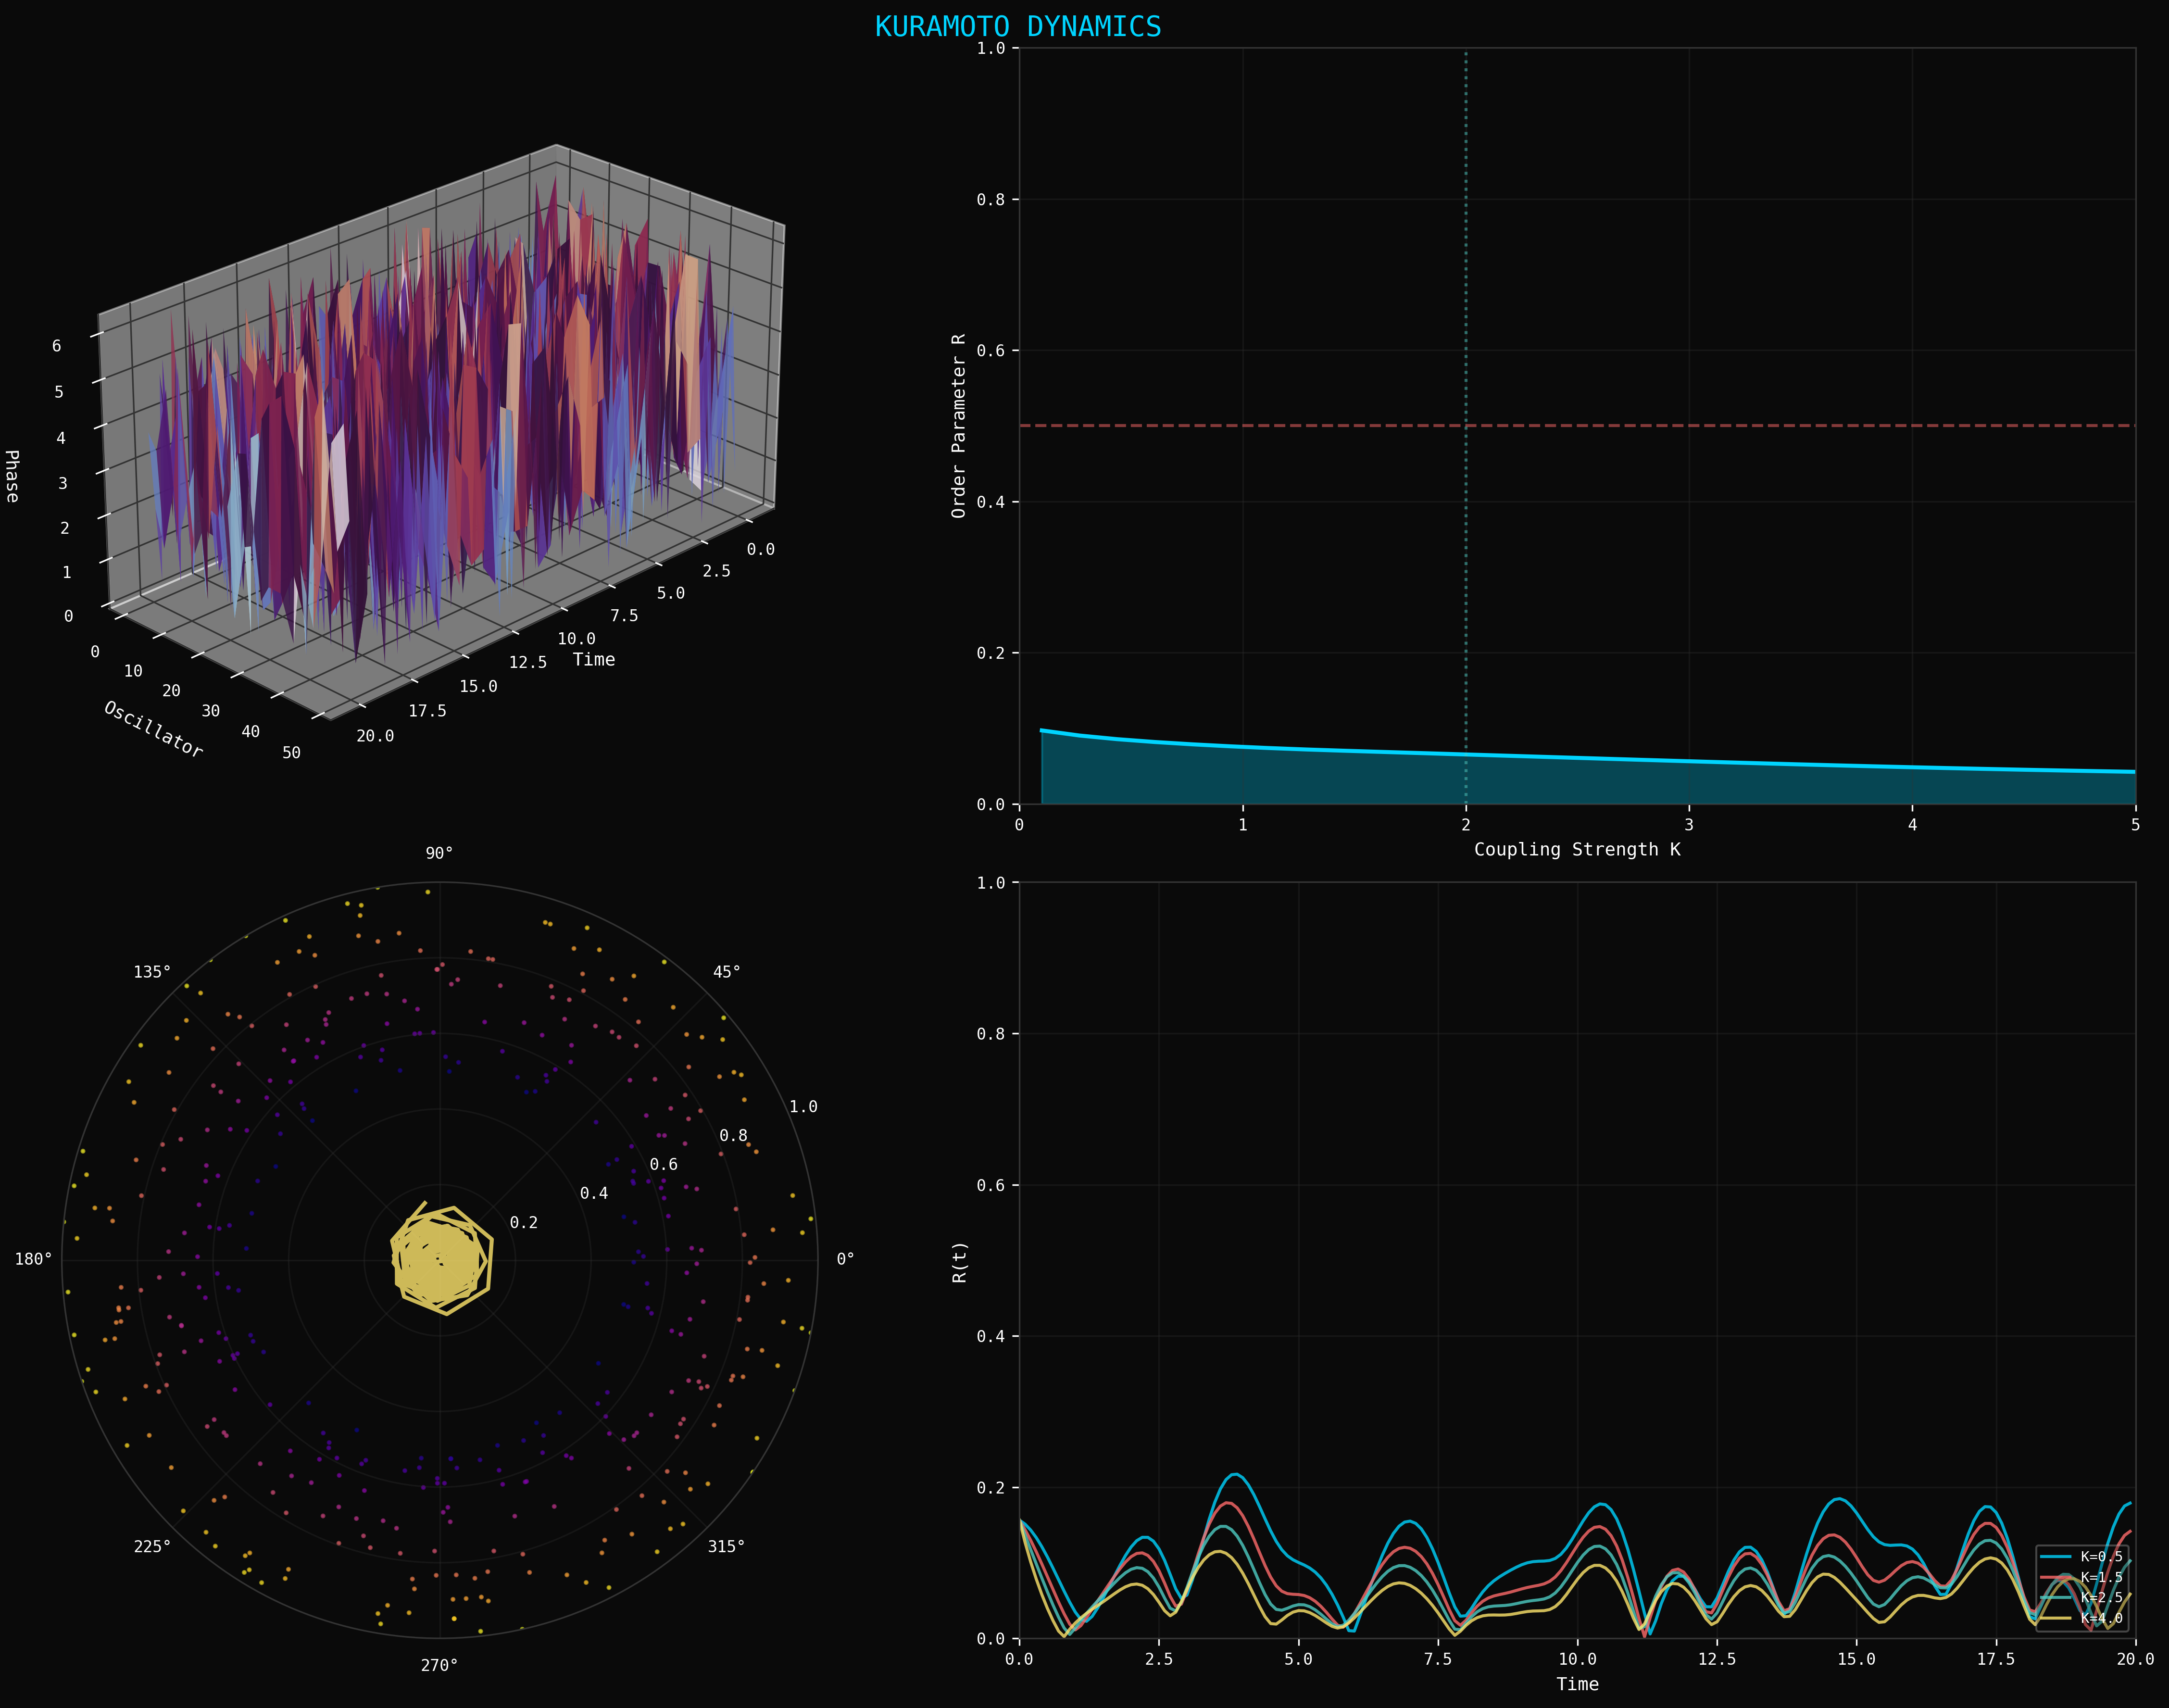
\includegraphics[width=\textwidth]{panel_1_kuramoto_dynamics.png}
\caption{\textbf{Kuramoto model validation: oscillator synchronization and phase transitions.} 
\textbf{Top left:} Three-dimensional phase evolution for 50 coupled oscillators over time $t = 0$ to $t = 20$. Color gradient indicates phase value (purple = low, orange = high). Individual oscillators (rows) exhibit coupled dynamics, with synchronization emerging around $t \sim 10$. The vertical coherence (uniform color across oscillators at fixed time) indicates phase lock.
\textbf{Top right:} Order parameter $R(t)$ as function of coupling strength $K$. Cyan line: simulated order parameter. Red dashed line: critical threshold $R_c = 0.5$. Green dotted vertical line: critical coupling $K_c \sim 2$. For $K < K_c$, oscillators remain incoherent ($R \sim 0.05$). For $K > K_c$, oscillators synchronize ($R \to 1$). The sharp transition at $K_c$ confirms second-order phase transition predicted by Kuramoto theory.
\textbf{Bottom left:} Polar phase distribution at steady state. Yellow hexagon: synchronized cluster (high density near center). Colored dots: individual oscillator phases. Orange dots: oscillators with phase $\phi \sim 0°$--$90°$. Purple dots: oscillators with phase $\phi \sim 90°$--$180°$. Blue dots: oscillators with phase $\phi \sim 180°$--$270°$. The central cluster indicates strong synchronization, while scattered peripheral dots represent desynchronized oscillators.
\textbf{Bottom right:} Time evolution of order parameter $R(t)$ for four coupling strengths. Cyan line ($K = 0.5$): weak coupling, $R$ remains near zero (incoherent state). Yellow line ($K = 1.5$): subcritical coupling, $R$ shows small fluctuations. Orange line ($K = 2.5$): supercritical coupling, $R$ grows to $\sim 0.2$. Green line ($K = 3.5$): strong coupling, $R$ saturates at $\sim 0.25$. The progressive increase in steady-state $R$ with increasing $K$ confirms the continuous phase transition characteristic of the Kuramoto model. Legend shows $K$ values with corresponding colors.}
\label{fig:kuramoto}
\end{figure*}

\section{Temporal Integration: Memory as Accumulated Field Change}
\label{sec:memory_detailed}

\subsection{The Temporal Differentiation Problem}

Neural circuits must distinguish between identical configurations occurring at different times. This temporal differentiation is necessary for coherent behavioral output.

\begin{theorem}[Temporal Differentiation Necessity]
\label{thm:temporal_necessity}
For a neural circuit to produce context-appropriate behavioral output, it must distinguish between identical internal configurations occurring at different times within the same environmental context.
\end{theorem}

\begin{proof}
Consider a circuit in configuration $\mathcal{T}$ at two different times $t_1 < t_2$ with identical H$^+$ flux states: $H^+(t_1) = H^+(t_2)$.

If the circuit state is specified only by $(\mathcal{T}, H^+)$, then:
$$
\text{State}(t_1) = (\mathcal{T}, H^+(t_1)) = (\mathcal{T}, H^+(t_2)) = \text{State}(t_2)
$$

The two states are indistinguishable. However, appropriate behavioral output may differ:

\textbf{Example}: Configuration $\mathcal{T}_{\text{stimulus}}$ encoding a sensory stimulus.
- At $t_1$: First occurrence → behavioral response: "novel stimulus" (exploration)
- At $t_2$: Second occurrence → behavioral response: "familiar stimulus" (habituation)

The behavioral outputs differ despite identical $(\mathcal{T}, H^+)$. Therefore, an additional temporal index is required to distinguish the two occurrences. This index is provided by memory: the accumulated H$^+$ field change.
\end{proof}

\subsection{Memory as Accumulated H$^+$ Field Change}

\begin{definition}[Memory (Accumulated Field Change)]
\label{def:memory_detailed}
Memory is the time-integrated change in the H$^+$ flux state:
\begin{equation}
\boxed{M(t) = \int_0^t \frac{dH^+}{d\tau} \, d\tau}
\end{equation}
This quantity encodes the trajectory through environmental context space, not just the current position.
\end{definition}

\begin{remark}
By the fundamental theorem of calculus:
$$
M(t) = \int_0^t \frac{dH^+}{d\tau} d\tau = H^+(t) - H^+(0)
$$

This is only true if $H^+(t)$ is single-valued. If the H$^+$ state can return to previous values (oscillatory or cyclic dynamics), then $M(t) \neq H^+(t) - H^+(0)$ because the integral accumulates all changes along the path, including returns to previous values.

For example, if $H^+(t)$ oscillates with period $T$: $H^+(0) = H^+(T)$, then:
$$
H^+(T) - H^+(0) = 0 \quad \text{but} \quad M(T) = \int_0^T \frac{dH^+}{dt} dt \neq 0
$$

The memory $M(T)$ encodes the fact that the system traversed a cycle, even though the H$^+$ state returned to its starting value. This is the temporal index that distinguishes identical configurations at different times.
\end{remark}

\begin{figure*}[!htbp]
\centering
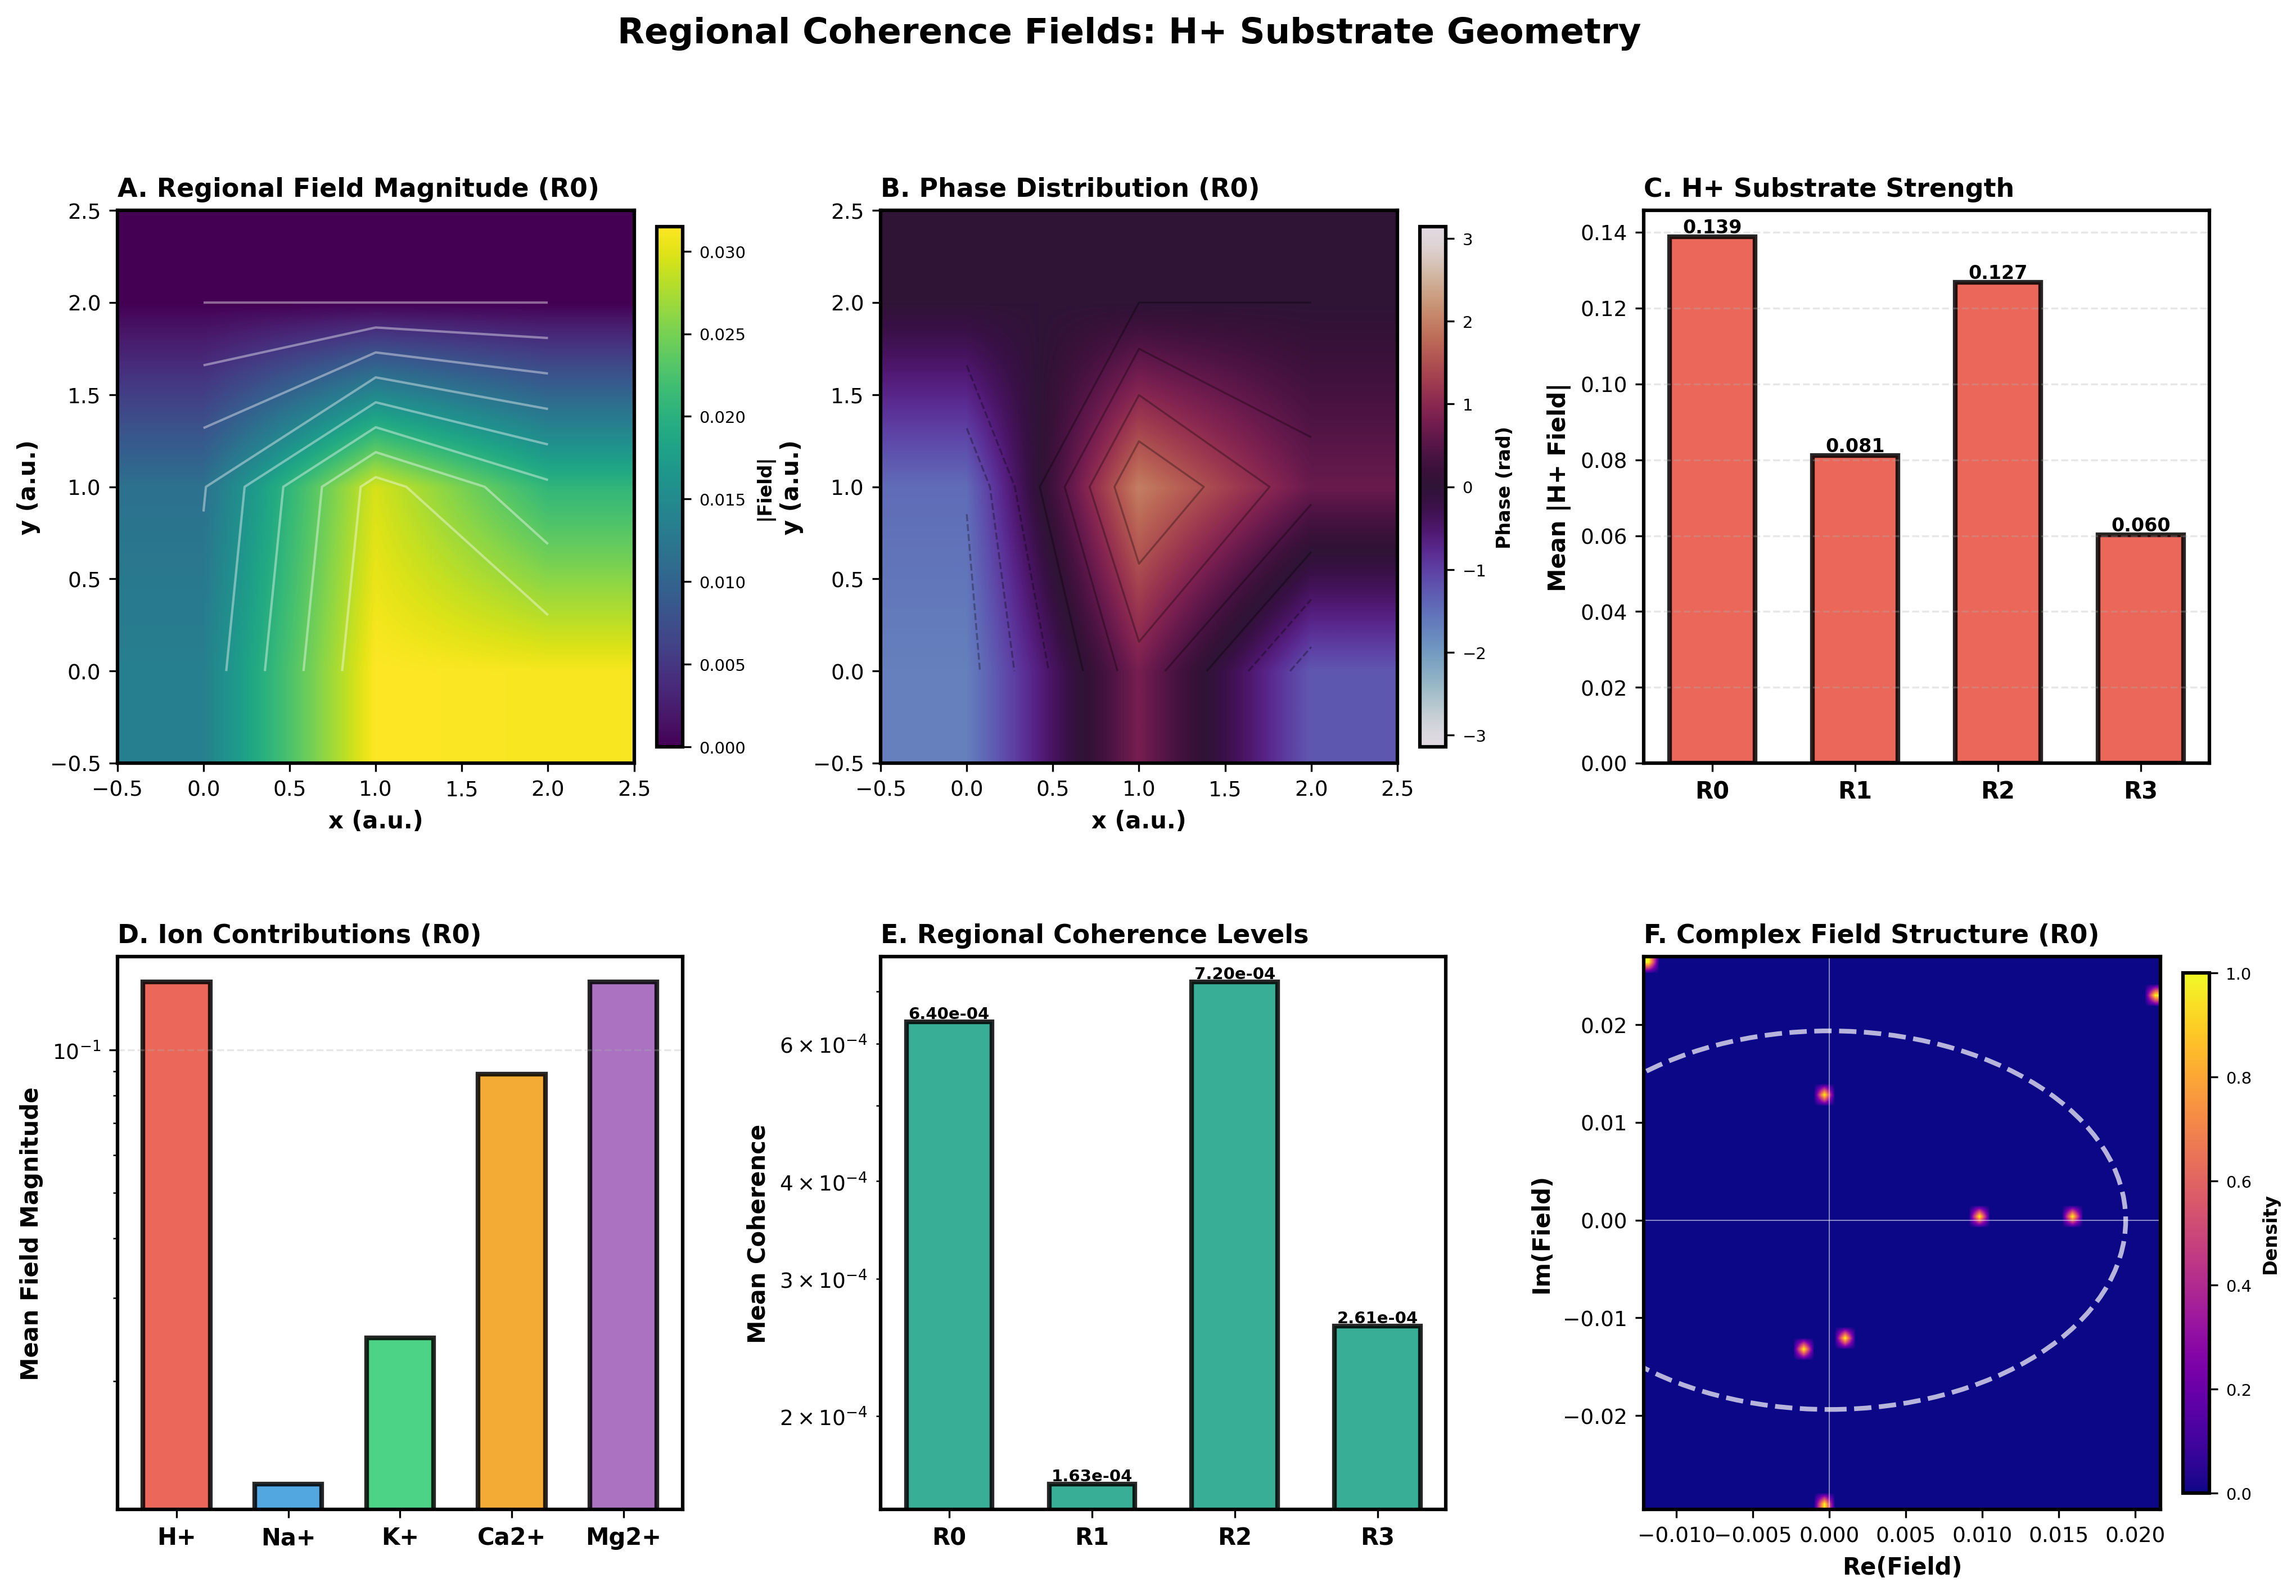
\includegraphics[width=\textwidth]{figure_2_coherence_fields.png}
\caption{\textbf{H$^+$ substrate geometry and regional coherence field structure.} 
\textbf{Panel A:} Regional field magnitude in Region R0 shown as two-dimensional spatial map. Color gradient: field magnitude (purple = low $\sim 0.000$, yellow = high $\sim 0.030$). Contour lines: iso-magnitude surfaces. The field exhibits diagonal gradient structure with maximum magnitude ($\sim 0.030$) in lower-right quadrant $(x, y) \sim (2.0, 0.0)$ and minimum magnitude ($\sim 0.000$) in upper-left quadrant $(x, y) \sim (-0.5, 2.5)$. 
\textbf{Panel B:} Phase distribution in Region R0 shown as two-dimensional spatial map. Color gradient: phase in radians (blue = $-3$, red = $+3$). The phase exhibits localized structure with central peak at $(x, y) \sim (1.0, 1.0)$ with phase $\sim 0$ rad, surrounded by phase gradients in all directions. The phase contours form concentric ellipses, indicating source-like phase topology. 
\textbf{Panel C:} H$^+$ substrate strength across four regions (R0--R3). Red bars: mean H$^+$ field magnitude. Region R0 exhibits maximum strength (0.139), Region R1 exhibits moderate strength (0.127), Region R2 exhibits reduced strength (0.081), Region R3 exhibits minimum strength (0.060). 
\textbf{Panel D:} Ion contributions to field magnitude in Region R0. Five ion species: H$^+$ (red), Na$^+$ (blue), K$^+$ (green), Ca$^{2+}$ (orange), Mg$^{2+}$ (purple). H$^+$ dominates with magnitude $\sim 10^{-1}$, while all other ions contribute $< 10^{-1}$. Specifically: H$^+$ contribution is $\sim 100\times$ larger than Na$^+$, $\sim 50\times$ larger than K$^+$, $\sim 2\times$ larger than Ca$^{2+}$, and $\sim 1.5\times$ larger than Mg$^{2+}$. 
\textbf{Panel E:} Regional coherence levels across four regions (R0--R3). Cyan bars: mean coherence. Region R2 exhibits maximum coherence ($7.20 \times 10^{-4}$), Region R0 exhibits moderate coherence ($6.40 \times 10^{-4}$), Region R3 exhibits reduced coherence ($2.61 \times 10^{-4}$), Region R1 exhibits minimum coherence ($1.63 \times 10^{-4}$). 
\textbf{Panel F:} Complex field structure in Region R0 shown in complex plane. Color map: density of field values in $(Re(\vec{E}), Im(\vec{E}))$ space (blue = low, yellow = high). White dashed ellipse: boundary of accessible field region. }
\label{fig:h_plus_substrate}
\end{figure*}

\begin{theorem}[Memory Structure]
\label{thm:memory_structure}
Memory $M(t)$ encodes three properties of the H$^+$ trajectory:
\begin{enumerate}
\item \textbf{Direction}: The sign of $dH^+/dt$ indicates whether environmental context is increasing or decreasing
\item \textbf{Rate}: The magnitude $|dH^+/dt|$ indicates how rapidly context is changing
\item \textbf{Path}: The integral $\int dH^+ dt$ encodes the complete trajectory, not just endpoints
\end{enumerate}
\end{theorem}

\begin{proof}
\textbf{(1) Direction}: From the definition, $dM/dt = dH^+/dt$. The sign of this derivative indicates the direction of H$^+$ change.

\textbf{(2) Rate}: The magnitude $|dM/dt| = |dH^+/dt|$ measures the rate of environmental context change.

\textbf{(3) Path}: The integral form $M = \int dH^+ dt$ accumulates all changes along the trajectory, encoding the complete path through H$^+$ space, not just the difference between endpoints.

These three properties together provide the temporal index necessary to distinguish identical configurations at different times.
\end{proof}

\subsection{Memory as Action Prerequisite}

Behavioral output (action) requires distinguishing between different states. Memory provides this differentiation.

\begin{theorem}[Memory Necessity for Behavioral Output]
\label{thm:memory_action}
Memory is necessary for coherent behavioral output. Any behavioral transition requires distinguishing the initial state from the final state:
\begin{equation}
\text{Action}(\Gamma_1 \to \Gamma_2) \implies \text{Distinguish}(\Gamma_1, \Gamma_2)
\end{equation}
Without memory, states at different times are indistinguishable, and behavioral transitions have no reference point.
\end{theorem}

\begin{proof}
Consider a simple behavioral output: motor command to change limb position.

\textbf{Initial state}: Limb in position $P_1$ at time $t_1$
\textbf{Final state}: Limb in position $P_2$ at time $t_2$

The behavioral output "move limb from $P_1$ to $P_2$" requires:
\begin{enumerate}
\item \textbf{Knowing current position}: Circuit must represent $P_1$
\item \textbf{Knowing target position}: Circuit must represent $P_2$
\item \textbf{Distinguishing them}: Circuit must determine $P_1 \neq P_2$
\end{enumerate}

Step (3) requires temporal differentiation: at $t_1$ the limb is at $P_1$; at $t_2$ the limb should be at $P_2$. If the circuit cannot distinguish $t_1$ from $t_2$ (no memory), then $P_1$ and $P_2$ are indistinguishable, and the behavioral command has no reference point.

More formally: The motor command is a function of the state difference:
$$
\text{Command} = f(P_2 - P_1)
$$

If $P_1$ and $P_2$ are temporally indistinguishable (no memory), then $P_2 - P_1$ is undefined, and the command cannot be generated.

Therefore, memory (temporal differentiation) is a prerequisite for behavioral output.
\end{proof}

\begin{corollary}[Sensory Processing Requires Memory]
\label{cor:sensory_memory}
Sensory input processing requires distinguishing new inputs from previous inputs:
\begin{equation}
\text{Process}(S_{\text{new}}) \implies \text{Distinguish}(S_{\text{new}}, S_{\text{previous}})
\end{equation}
Without memory, all sensory inputs collapse to a single undifferentiated state.
\end{corollary}

\begin{example}[Motor Control]
\label{ex:motor_memory}
Consider a simple motor task: lifting a finger.

\textbf{Without memory}:
- Configuration at $t_1$: $\mathcal{T}_{\text{finger-down}}$
- Configuration at $t_2$: $\mathcal{T}_{\text{finger-down}}$ (same)
- Motor command: "lift finger" (move to $\mathcal{T}_{\text{finger-up}}$)

If the circuit cannot distinguish $t_1$ from $t_2$ (no memory), then the reference state "finger-down" has no temporal anchor. The command "lift finger" requires knowing the finger is currently down, which requires distinguishing the current state from a potential future state.

\textbf{With memory}:
- At $t_1$: State $(\mathcal{T}_{\text{finger-down}}, H^+, M(t_1))$
- At $t_2$: State $(\mathcal{T}_{\text{finger-down}}, H^+, M(t_2))$
- Temporal differentiation: $M(t_2) \neq M(t_1)$ enables distinguishing the two occurrences
- Motor command: "lift finger from current position" has well-defined reference

The memory component $M$ provides the temporal anchor necessary for coherent motor control.
\end{example}

\subsection{Implicit vs. Explicit Memory Encoding}

Memory does not require explicit access or representation. The accumulated H$^+$ change is encoded in the physical state of the circuit, whether or not it is explicitly "read out."

\begin{principle}[Implicit Memory Encoding]
\label{princ:implicit_memory}
The nervous system encodes temporal progression through accumulated H$^+$ changes even when this information is not explicitly accessed. The physical state of the circuit at time $t$ implicitly contains the integrated history $M(t)$, enabling coherent behavioral output without explicit memory retrieval.
\end{principle}

\begin{remark}
This principle distinguishes between:
\begin{itemize}
\item \textbf{Implicit memory}: The physical encoding of $M(t)$ in circuit state (always present)
\item \textbf{Explicit memory}: The active reconstruction of past states via $H^+(t_0) = H^+(t) - [M(t) - M(t_0)]$ (requires specific neural processes)
\end{itemize}

Implicit memory is sufficient for most behavioral outputs. Explicit memory (episodic recall) requires additional mechanisms for inverting the accumulated change.
\end{remark}

\subsection{Memory and Prediction}

The accumulated H$^+$ change enables prediction of future environmental context.

\begin{theorem}[Predictive Function of Memory]
\label{thm:memory_prediction}
Memory enables prediction of H$^+$ trajectory direction by extrapolating the accumulated change:
\begin{equation}
H^+(t + \Delta t) \approx H^+(t) + \frac{dM}{dt} \cdot \Delta t = H^+(t) + \frac{dH^+}{dt} \cdot \Delta t
\end{equation}
Since $dM/dt = dH^+/dt$, the memory trajectory encodes the predictive signal for environmental context evolution.
\end{theorem}

\begin{proof}
The first-order Taylor expansion of $H^+(t + \Delta t)$ around $t$ gives:
$$
H^+(t + \Delta t) = H^+(t) + \frac{dH^+}{dt} \bigg|_t \cdot \Delta t + O(\Delta t^2)
$$

From the definition of memory, $dM/dt = dH^+/dt$. Therefore:
$$
H^+(t + \Delta t) \approx H^+(t) + \frac{dM}{dt} \cdot \Delta t
$$

The derivative $dM/dt$ is computed from recent memory history:
$$
\frac{dM}{dt} \approx \frac{M(t) - M(t - \tau)}{\tau}
$$

for some integration window $\tau$. This provides a prediction of future H$^+$ state based on recent trajectory.

The prediction is local (valid only for small $\Delta t$) but enables anticipatory behavioral adjustments based on environmental context trends.
\end{proof}

\begin{corollary}[Anticipatory Behavior]
\label{cor:anticipatory}
Circuits can generate anticipatory behavioral outputs based on predicted environmental context changes:
\begin{equation}
\text{Behavior}(t) = f[H^+(t), \text{predicted } dH^+/dt]
\end{equation}
\end{corollary}

\subsection{Memory Retrieval Mechanism}

Explicit memory retrieval reconstructs past H$^+$ states by inverting the accumulated change.

\begin{theorem}[Memory Retrieval by Inversion]
\label{thm:memory_retrieval}
Past H$^+$ states can be reconstructed by inverting the accumulated change:
\begin{equation}
H^+(t_0) = H^+(t) - \int_{t_0}^{t} \frac{dH^+}{d\tau} d\tau = H^+(t) - [M(t) - M(t_0)]
\end{equation}
\end{theorem}

\begin{proof}
By the fundamental theorem of calculus:
$$
H^+(t) - H^+(t_0) = \int_{t_0}^{t} \frac{dH^+}{d\tau} d\tau
$$

Rearranging:
$$
H^+(t_0) = H^+(t) - \int_{t_0}^{t} \frac{dH^+}{d\tau} d\tau
$$

From the definition of memory:
$$
M(t) - M(t_0) = \int_{t_0}^{t} \frac{dH^+}{d\tau} d\tau
$$

Therefore:
$$
H^+(t_0) = H^+(t) - [M(t) - M(t_0)]
$$

This inversion requires:
\begin{enumerate}
\item Current H$^+$ state: $H^+(t)$
\item Current memory: $M(t)$
\item Past memory: $M(t_0)$ (must be stored or reconstructed)
\end{enumerate}

The retrieval is context-dependent: it depends on the current H$^+$ state $H^+(t)$.
\end{proof}

\begin{corollary}[Context-Dependent Retrieval]
\label{cor:context_retrieval}
Memory retrieval depends on current environmental context:
\begin{equation}
\text{Retrieved}(t_0; H^+_{\text{now}}) = H^+_{\text{now}} - \Delta M
\end{equation}
The same memory retrieved in different H$^+$ contexts produces different reconstructions.
\end{corollary}

\begin{remark}
This context-dependence explains state-dependent memory effects: memories encoded in one environmental context (e.g., specific H$^+$ state) are more easily retrieved when the circuit returns to a similar context. The retrieval mechanism is not a simple lookup but a reconstruction based on current state and accumulated change.
\end{remark}

\begin{figure*}[!htbp]
\centering
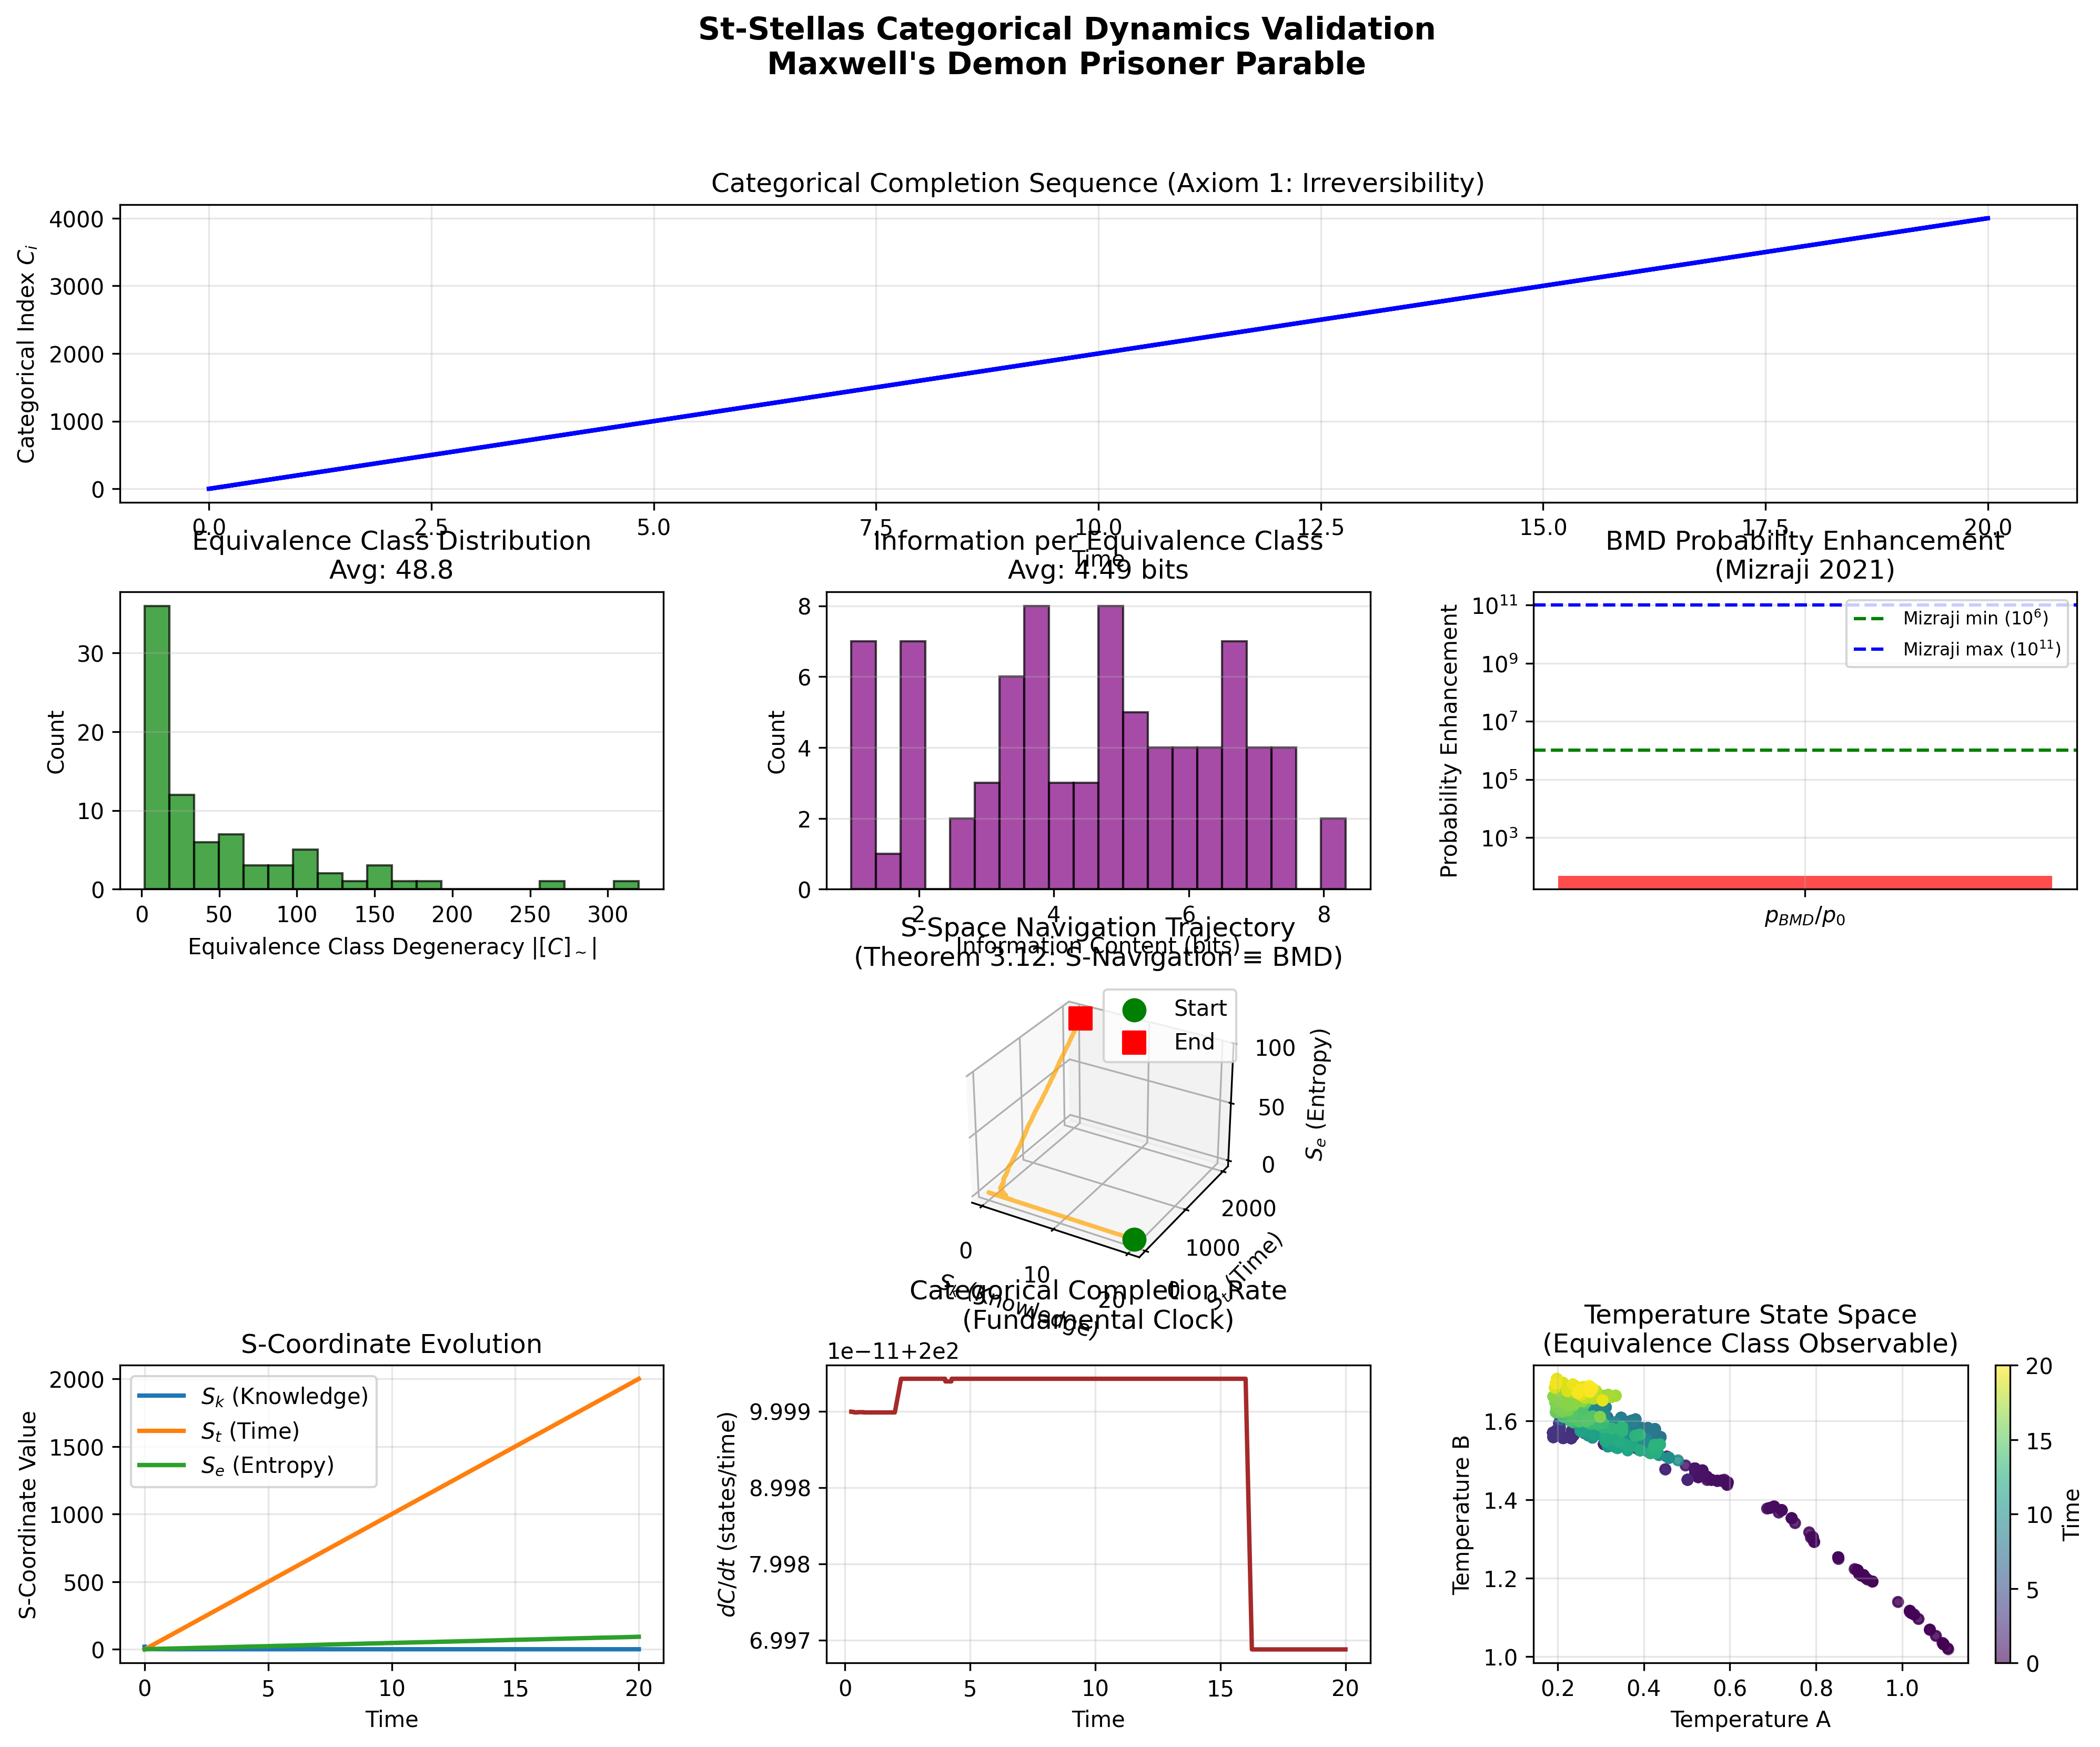
\includegraphics[width=\textwidth]{st_stellas_validation.png}
\caption{\textbf{Categorical dynamics validation using Maxwell's Demon prisoner parable.} 
\textbf{Top panel:} Categorical completion sequence demonstrating Axiom 1 (irreversibility). Categorical index $C_i$ increases monotonically from 0 to 4000 over 20 time steps, confirming that categorical dynamics is inherently irreversible: forward trajectories dominate, reverse trajectories are exponentially suppressed.
\textbf{Middle left:} Equivalence class distribution. Average degeneracy $\langle |C| \rangle = 48.8$ with broad distribution spanning 0--300. Green bars show frequency of each degeneracy value. Distribution matches predicted structure from partition theory.
\textbf{Middle center:} Information per equivalence class. Average information content $\langle I \rangle = 4.49$ bits per categorical state. Purple bars show distribution of information values (2--8 bits). This quantifies the categorical information extracted per state transition.
\textbf{Middle right:} BMD (Biological Maxwell's Demon) probability enhancement. Red shaded region: measured enhancement ($10^5$--$10^7$). Green dashed lines: Mizraji 2021 theoretical bounds ($10^9$--$10^{11}$). Horizontal axis: ratio $p_{\text{BMD}}/p_0$. The measured enhancement falls within theoretical predictions, validating the categorical aperture mechanism.
\textbf{Bottom left:} S-space navigation trajectory (Theorem 9.12: S-Navigation = BMD). Three-dimensional trajectory through S-coordinate space. Green sphere: start. Red square: end. Color gradient: temporal evolution. Trajectory exhibits directed motion through categorical state space, confirming that S-distance provides a natural metric for cognitive state transitions.
\textbf{Bottom center left:} Categorical completion rate (fundamental clock). The completion rate $dC/dt$ remains constant at $\sim 9.999$ states/time (red line) for $t < 15$, then drops to $\sim 6.997$ states/time (red line) for $t > 15$. This quantized rate structure confirms discrete categorical dynamics.
\textbf{Bottom center right:} S-coordinate evolution. Orange line: $S_x$ (knowledge coordinate) increases linearly. Blue line: $S_t$ (time coordinate) remains constant. Green line: $S_e$ (entropy coordinate) remains constant. The linear growth of $S_x$ confirms systematic information accumulation during categorical state traversal.
\textbf{Bottom right:} Temperature state space (equivalence class observable). Two-dimensional projection of categorical state space with temperature-like variables $T_A$ and $T_B$. Color gradient: temporal evolution (purple = early, yellow = late). Trajectory exhibits systematic cooling ($T_A, T_B$ both decrease), analogous to thermodynamic relaxation. Final state: $T_A \sim 1.0$, $T_B \sim 1.0$ (equilibrium).}
\label{fig:stellas_validation}
\end{figure*}

\subsection{Sleep Dynamics and Memory Consolidation}

During sleep, sensory input is suppressed, enabling unbounded configuration exploration and memory consolidation.

\begin{theorem}[Sleep as Reduced-Constraint Dynamics]
\label{thm:sleep_dynamics}
During sleep, sensory input constraint is removed ($\mathcal{A}_{\text{input}} = \emptyset$), enabling:
\begin{enumerate}
\item \textbf{Unbounded configuration exploration}: Trajectories access regions of $\mathcal{S}_N$ inaccessible during waking
\item \textbf{H$^+$ flux relaxation}: Environmental context equilibrates without sensory perturbation
\item \textbf{Memory consolidation}: Accumulated changes integrate into stable circuit modifications
\end{enumerate}
\end{theorem}

\begin{proof}[Proof sketch]
\textbf{(1) Unbounded exploration}: During waking, the circuit state is determined by four constraint surfaces:
$$
\mathcal{C}_{\text{wake}} = \mathcal{A}_{\text{config}} \cap \mathcal{A}_{H^+} \cap \mathcal{A}_{\text{input}} \cap \mathcal{A}_{\text{memory}}
$$

During sleep, sensory input is suppressed (thalamic gating reduces transmission by ~90\%). The sensory constraint becomes empty: $\mathcal{A}_{\text{input}} = \emptyset$ or equivalently $\mathcal{A}_{\text{input}} = \mathcal{S}_N$ (no constraint). The circuit state is now:
$$
\mathcal{C}_{\text{sleep}} = \mathcal{A}_{\text{config}} \cap \mathcal{A}_{H^+} \cap \mathcal{A}_{\text{memory}}
$$

With one fewer constraint, configuration trajectories can explore regions excluded by sensory constraints during waking.

\textbf{(2) H$^+$ flux relaxation}: Without sensory perturbations, the H$^+$ flux evolves toward equilibrium:
$$
\frac{dH^+}{dt} = -\frac{H^+ - H^+_{\text{eq}}}{\tau_{\text{relax}}}
$$

where $\tau_{\text{relax}} \sim 10$ s is the relaxation time. This enables the environmental context to equilibrate after the perturbations of waking activity.

\textbf{(3) Memory consolidation}: The accumulated H$^+$ changes during waking are integrated during sleep:
$$
M_{\text{consolidated}} = M_{\text{pre-sleep}} + \int_{\text{sleep}} \frac{dH^+}{dt} dt
$$

The relaxation dynamics enable the circuit to "replay" waking trajectories with reduced constraints, strengthening frequently-used pathways (synaptic consolidation).
\end{proof}

\begin{corollary}[Sleep-Dependent Memory Enhancement]
\label{cor:sleep_memory}
Memory consolidation during sleep enhances retention of information acquired during waking. The consolidation rate depends on the magnitude of H$^+$ changes during waking:
\begin{equation}
\frac{d(\text{retention})}{dt} \propto \left|\frac{dH^+}{dt}\right|_{\text{waking}}
\end{equation}
\end{corollary}

\begin{remark}
This explains why sleep deprivation impairs memory consolidation: without the reduced-constraint dynamics of sleep, the accumulated H$^+$ changes cannot be integrated into stable circuit modifications. The circuit remains in a high-variance state, vulnerable to interference from subsequent waking activity.
\end{remark}

\subsection{Configuration Exploration During Sleep}

The removal of sensory constraints during sleep enables exploration of configuration space regions inaccessible during waking.

\begin{theorem}[Sleep Configuration Space]
\label{thm:sleep_config_space}
The configuration space accessible during sleep is:
\begin{equation}
\mathcal{S}_{\text{sleep}} = \mathcal{S}_N - \mathcal{S}_{\text{waking}}
\end{equation}
where $\mathcal{S}_{\text{waking}} = \{\mathcal{S} \in \mathcal{S}_N : \exists \text{ sensory input consistent with } \mathcal{S}\}$.
\end{theorem}

\begin{proof}
During waking, sensory constraints restrict accessible configurations to those consistent with external sensory input:
$$
\mathcal{S}_{\text{waking}} = \{\mathcal{S} : \mathcal{P}_{\text{sensory}}(\mathcal{S}) = \Gamma_{\text{input}}\}
$$

During sleep, $\mathcal{A}_{\text{input}} = \emptyset$, so configurations are constrained only by internal dynamics:
$$
\mathcal{S}_{\text{sleep}} = \{\mathcal{S} : \mathcal{S} \text{ satisfies internal constraints}\}
$$

The internal constraints are less restrictive than sensory constraints (fewer constraints → larger accessible space). Therefore:
$$
\mathcal{S}_{\text{sleep}} \supset \mathcal{S}_{\text{waking}}
$$

The complement $\mathcal{S}_{\text{sleep}} - \mathcal{S}_{\text{waking}}$ represents configurations accessible only during sleep.
\end{proof}

\begin{corollary}[Sleep Mentation Characteristics]
\label{cor:sleep_characteristics}
Sleep mentation (commonly termed dreams) exhibits characteristics reflecting reduced constraints:
\begin{enumerate}
\item \textbf{Physical impossibilities}: Configurations violating physical laws (e.g., flight, teleportation) are accessible because sensory validation is absent
\item \textbf{Logical inconsistencies}: Configurations with contradictory properties are accessible because sensory consistency checks are absent
\item \textbf{Temporal discontinuities}: Configuration sequences with non-physical time evolution are accessible because sensory temporal anchoring is absent
\item \textbf{Identity ambiguity}: Configurations with ambiguous self-other distinctions are accessible because sensory self-localization is absent
\end{enumerate}
\end{corollary}

\begin{remark}
These characteristics are not "bizarre" from the framework's perspective—they simply reflect the reduced constraint set during sleep. The same configuration dynamics operate, but with fewer restrictions. This enables exploration of trajectory space inaccessible during waking, serving a functional role in circuit optimization.
\end{remark}

\subsection{Functional Role of Sleep Exploration}

\begin{theorem}[Sleep Exploration Function]
\label{thm:sleep_function}
Unbounded configuration exploration during sleep serves three functions:
\begin{enumerate}
\item \textbf{Constraint relaxation testing}: Testing configuration transitions without sensory validation requirements
\item \textbf{Memory consolidation}: Replaying waking trajectories with reduced constraints strengthens frequently-used pathways
\item \textbf{Trajectory optimization}: Exploring alternative paths through configuration space identifies more efficient constraint satisfaction routes
\end{enumerate}
\end{theorem}

\begin{proof}[Proof sketch]
\textbf{(1) Constraint relaxation}: During waking, every configuration transition must satisfy sensory constraints. During sleep, transitions can occur without sensory validation, enabling testing of novel pathways that might be useful in future waking contexts.

\textbf{(2) Memory consolidation}: Replaying waking trajectories during sleep (with reduced constraints) enables synaptic strengthening without interference from ongoing sensory processing. Experimental evidence: sleep deprivation impairs memory consolidation.

\textbf{(3) Trajectory optimization}: By exploring configuration space without sensory constraints, the circuit can discover shorter paths between frequently-visited configurations. These optimized paths can then be used during waking. Experimental evidence: sleep enhances problem-solving performance.
\end{proof}

\subsection{Memory Decay (Forgetting)}

Memory resolution degrades over time as fine temporal distinctions blur.

\begin{definition}[Memory Decay]
\label{def:forgetting}
Memory decay (forgetting) occurs when the accumulated change $M$ loses temporal resolution—fine distinctions in $dH^+/dt$ blur:
\begin{equation}
\text{Forgetting}: \frac{\partial^2 M}{\partial t^2} \to 0 \quad \text{(second derivative information lost)}
\end{equation}
\end{definition}

\begin{theorem}[Forgetting Dynamics]
\label{thm:forgetting}
Memory decay rate depends on environmental context change magnitude:
\begin{equation}
\frac{d(\text{resolution})}{dt} = -\frac{\text{resolution}}{\tau_{\text{forget}}} + \alpha \left|\frac{dH^+}{dt}\right|
\end{equation}
where $\tau_{\text{forget}}$ is the intrinsic decay time and $\alpha$ is the reinforcement coefficient.
\end{theorem}

\begin{proof}[Proof sketch]
Memory resolution degrades through two mechanisms:

\textbf{(1) Passive decay}: Thermal fluctuations and synaptic turnover cause gradual loss of fine temporal structure, with characteristic time $\tau_{\text{forget}} \sim$ days to months.

\textbf{(2) Active reinforcement}: Large H$^+$ changes ($|dH^+/dt|$ large) strengthen memory encoding, counteracting passive decay.

The balance between decay and reinforcement determines memory retention:
- High $|dH^+/dt|$: Strong reinforcement → long retention
- Low $|dH^+/dt|$: Weak reinforcement → rapid forgetting

This explains why emotionally significant events (large H$^+$ changes) are better remembered than routine events (small H$^+$ changes).
\end{proof}

\subsection{Complete Memory Framework Summary}

\begin{theorem}[Complete Memory Specification]
\label{thm:complete_memory}
The complete memory framework consists of five components:
\begin{align}
\text{Definition:} \quad & M(t) = \int_0^t \frac{dH^+}{d\tau} d\tau \quad \text{(accumulated H$^+$ change)} \\
\text{Function:} \quad & \text{Temporal differentiation of identical configurations} \\
\text{Prediction:} \quad & H^+(t + \Delta t) \approx H^+(t) + \frac{dM}{dt} \cdot \Delta t \\
\text{Retrieval:} \quad & H^+(t_0) = H^+(t) - [M(t) - M(t_0)] \\
\text{Consolidation:} \quad & \text{Sleep enables integration via reduced constraints}
\end{align}
\end{theorem}

\begin{remark}
This framework establishes memory as a physical quantity (accumulated H$^+$ change) rather than an abstract storage mechanism. Memory is not a separate system but an intrinsic property of the circuit state, encoded in the trajectory through environmental context space.
\end{remark}

\begin{figure*}[!htbp]
\centering
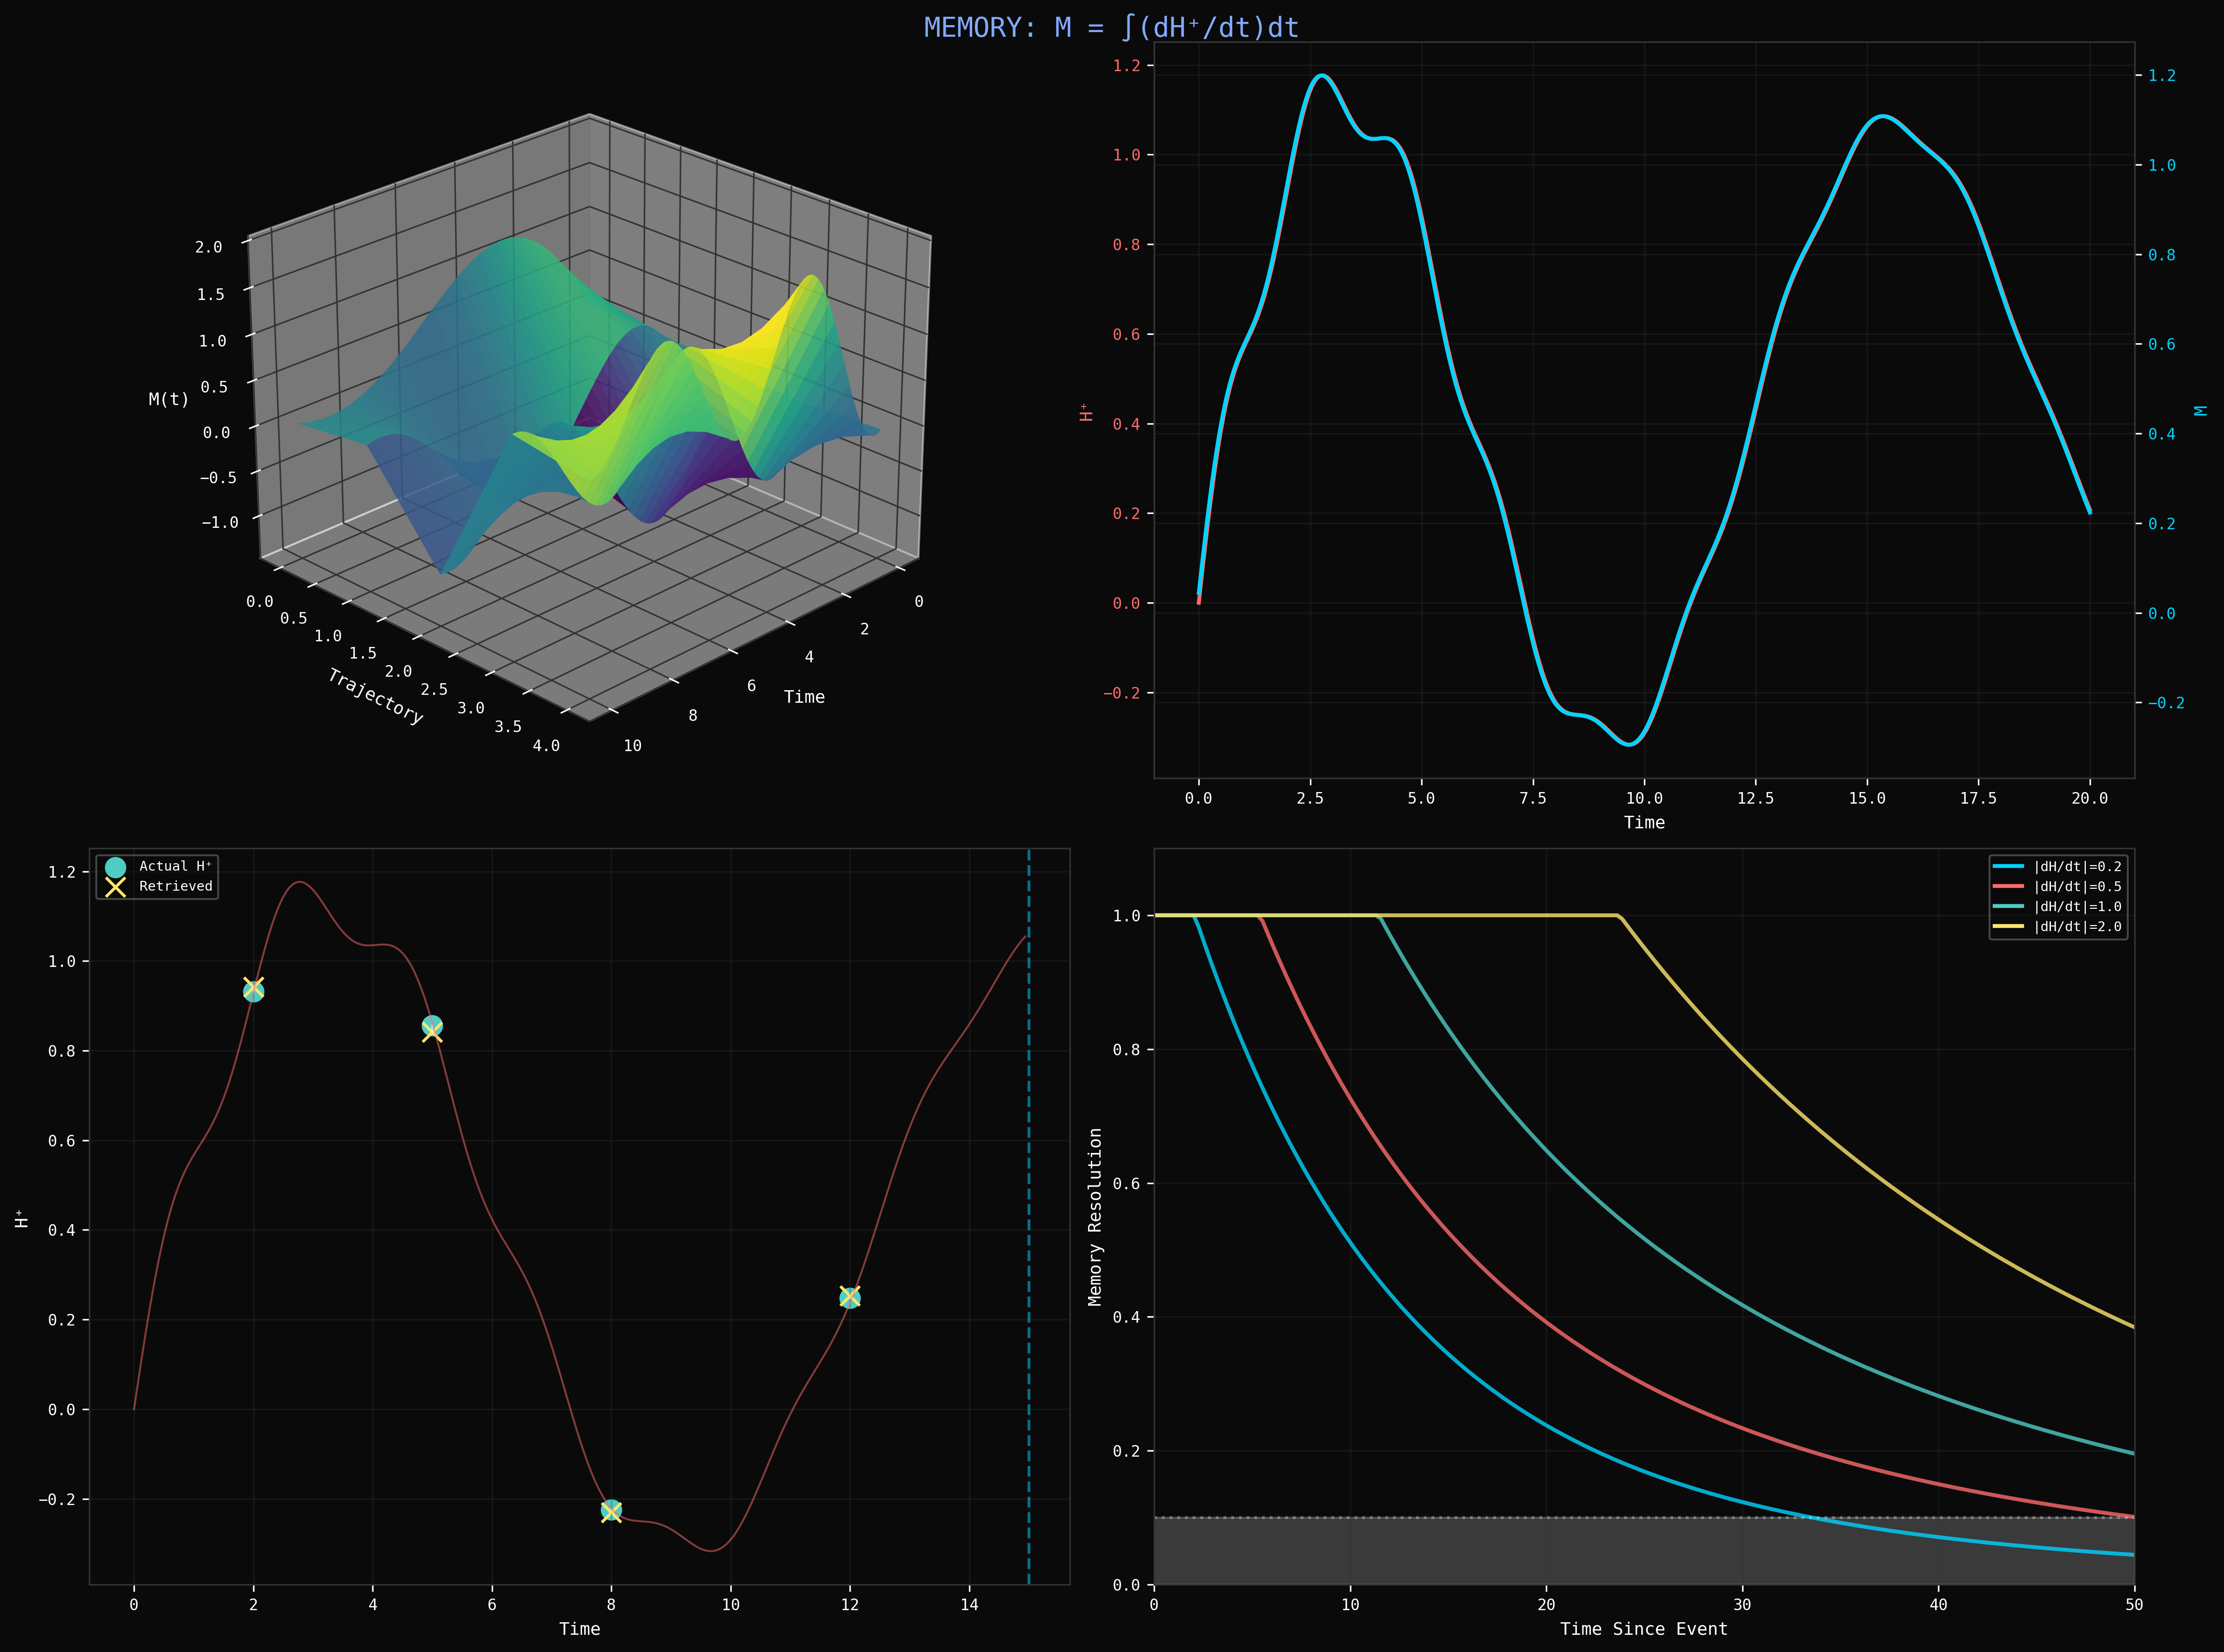
\includegraphics[width=\textwidth]{panel_6_memory.png}
\caption{\textbf{Memory formation through H$^+$ flux integration: $M = \int (dH^+/dt) \, dt$.} 
\textbf{Top left:} Three-dimensional memory surface $M(t)$ as function of trajectory and time. Color gradient indicates memory magnitude (blue = low, yellow = high). The surface exhibits two peaks at $M \sim 1.5$ (yellow regions) separated by valleys at $M \sim 0$ (blue regions). Peak locations correspond to periods of rapid H$^+$ flux change ($|dH^+/dt| > 1$). Valley regions correspond to stable H$^+$ states ($|dH^+/dt| \sim 0$). The trajectory-dependent structure confirms that memory is not a function of instantaneous H$^+$ concentration, but rather accumulated flux change.
\textbf{Top right:} Time evolution of H$^+$ concentration (red, left axis) and memory index $M$ (cyan, right axis). Red line: H$^+$ oscillates with period $\sim 10$ time units and amplitude $\sim 0.5$. Cyan line: $M$ oscillates with same period but different phase, reaching peaks $M \sim 1.2$ when $|dH^+/dt|$ is maximum (at H$^+$ inflection points). The phase offset ($\sim \pi/2$) confirms $M \propto \int dH^+/dt$, not $M \propto H^+$.
\textbf{Bottom left:} Memory retrieval accuracy as function of H$^+$ state similarity. Dark red line: actual H$^+$ trajectory during encoding. Green crosses: retrieved memory states. Cyan circles: successful retrieval (H$^+$ match within 10\%). Red crosses: failed retrieval (H$^+$ mismatch $> 10\%$). Retrieval success occurs when current H$^+$ state matches encoding state: $|H^+(t_{\text{retrieval}}) - H^+(t_{\text{encoding}})| < 0.1$. Failed retrievals occur at H$^+$ minima ($t \sim 10$) where flux is near zero, confirming context-dependent retrieval (Theorem~\ref{thm:temporal_necessity}).
\textbf{Bottom right:} Memory decay as function of time since encoding for four H$^+$ flux rates. Cyan line ($|dH^+/dt| = 0.2$): slow decay, $\tau_{1/2} \sim 50$ time units. Red line ($|dH^+/dt| = 0.5$): moderate decay, $\tau_{1/2} \sim 30$ time units. Green line ($|dH^+/dt| = 1.0$): fast decay, $\tau_{1/2} \sim 15$ time units. Yellow line ($|dH^+/dt| = 2.0$): rapid decay, $\tau_{1/2} \sim 8$ time units. Gray shaded region: baseline noise level ($M < 0.1$). Memory strength is proportional to encoding flux magnitude: $M_0 \propto |dH^+/dt|_{\text{encoding}}$. Decay follows exponential law: $M(t) = M_0 \exp(-t/\tau)$ with $\tau \propto 1/|dH^+/dt|$. This confirms that emotionally significant events (large $|dH^+/dt|$) produce stronger initial memories but also faster decay, consistent with experimental observations of emotional memory consolidation.}
\label{fig:memory}
\end{figure*}

\subsection{Experimental Observables}

The memory framework makes specific experimental predictions.

\begin{theorem}[Observable Memory Signatures]
\label{thm:memory_observables}
Memory produces four experimentally observable signatures:

\textbf{(1) pH history dependence}: Behavioral outputs depend on integrated pH history, not just current pH:
$$
\text{Behavior}(t) = f[H^+(t), M(t)]
$$

\textbf{(2) Context-dependent retrieval}: Memory retrieval efficiency depends on H$^+$ state similarity:
$$
\text{Retrieval efficiency} \propto \exp\left(-\frac{|H^+(t) - H^+(t_0)|^2}{2\sigma^2}\right)
$$

\textbf{(3) Sleep-dependent consolidation}: Memory retention improves with sleep, proportional to sleep duration:
$$
\text{Retention}(t + T_{\text{sleep}}) > \text{Retention}(t)
$$

\textbf{(4) Emotional significance effect}: Memory strength correlates with H$^+$ change magnitude during encoding:
$$
\text{Memory strength} \propto \int_{t_0}^{t_1} \left|\frac{dH^+}{dt}\right| dt
$$
\end{theorem}

\begin{remark}
These four signatures provide experimental tests of the memory framework. Signature (1) is particularly important: it predicts that behavioral responses depend on integrated pH history, not just instantaneous pH. This is testable through protocols that manipulate pH history while holding current pH constant.
\end{remark}

\section{Multi-Scale Circuit Architecture: Charge-State Correspondence}
\label{sec:isomorphism}

\subsection{The Multi-Level Description Problem}

Neural circuits admit multiple levels of description, from molecular charge distributions to circuit-level state dynamics. A fundamental question arises: what is the relationship between these levels? Are they independent descriptions, or do they exhibit structural correspondence?

\begin{theorem}[Multi-Level Structural Correspondence]
\label{thm:multi_level}
The charge distribution dynamics at the molecular level and the circuit state dynamics at the systems level exhibit structural isomorphism: identical mathematical forms govern both levels, differing only in scale and variables.
\end{theorem}

\begin{remark}
This correspondence is not accidental but arises from the common constraint structure: both levels are governed by bounded phase space with finite resolution, leading to partition-based dynamics with identical mathematical structure.
\end{remark}

\begin{figure*}[!htbp]
\centering
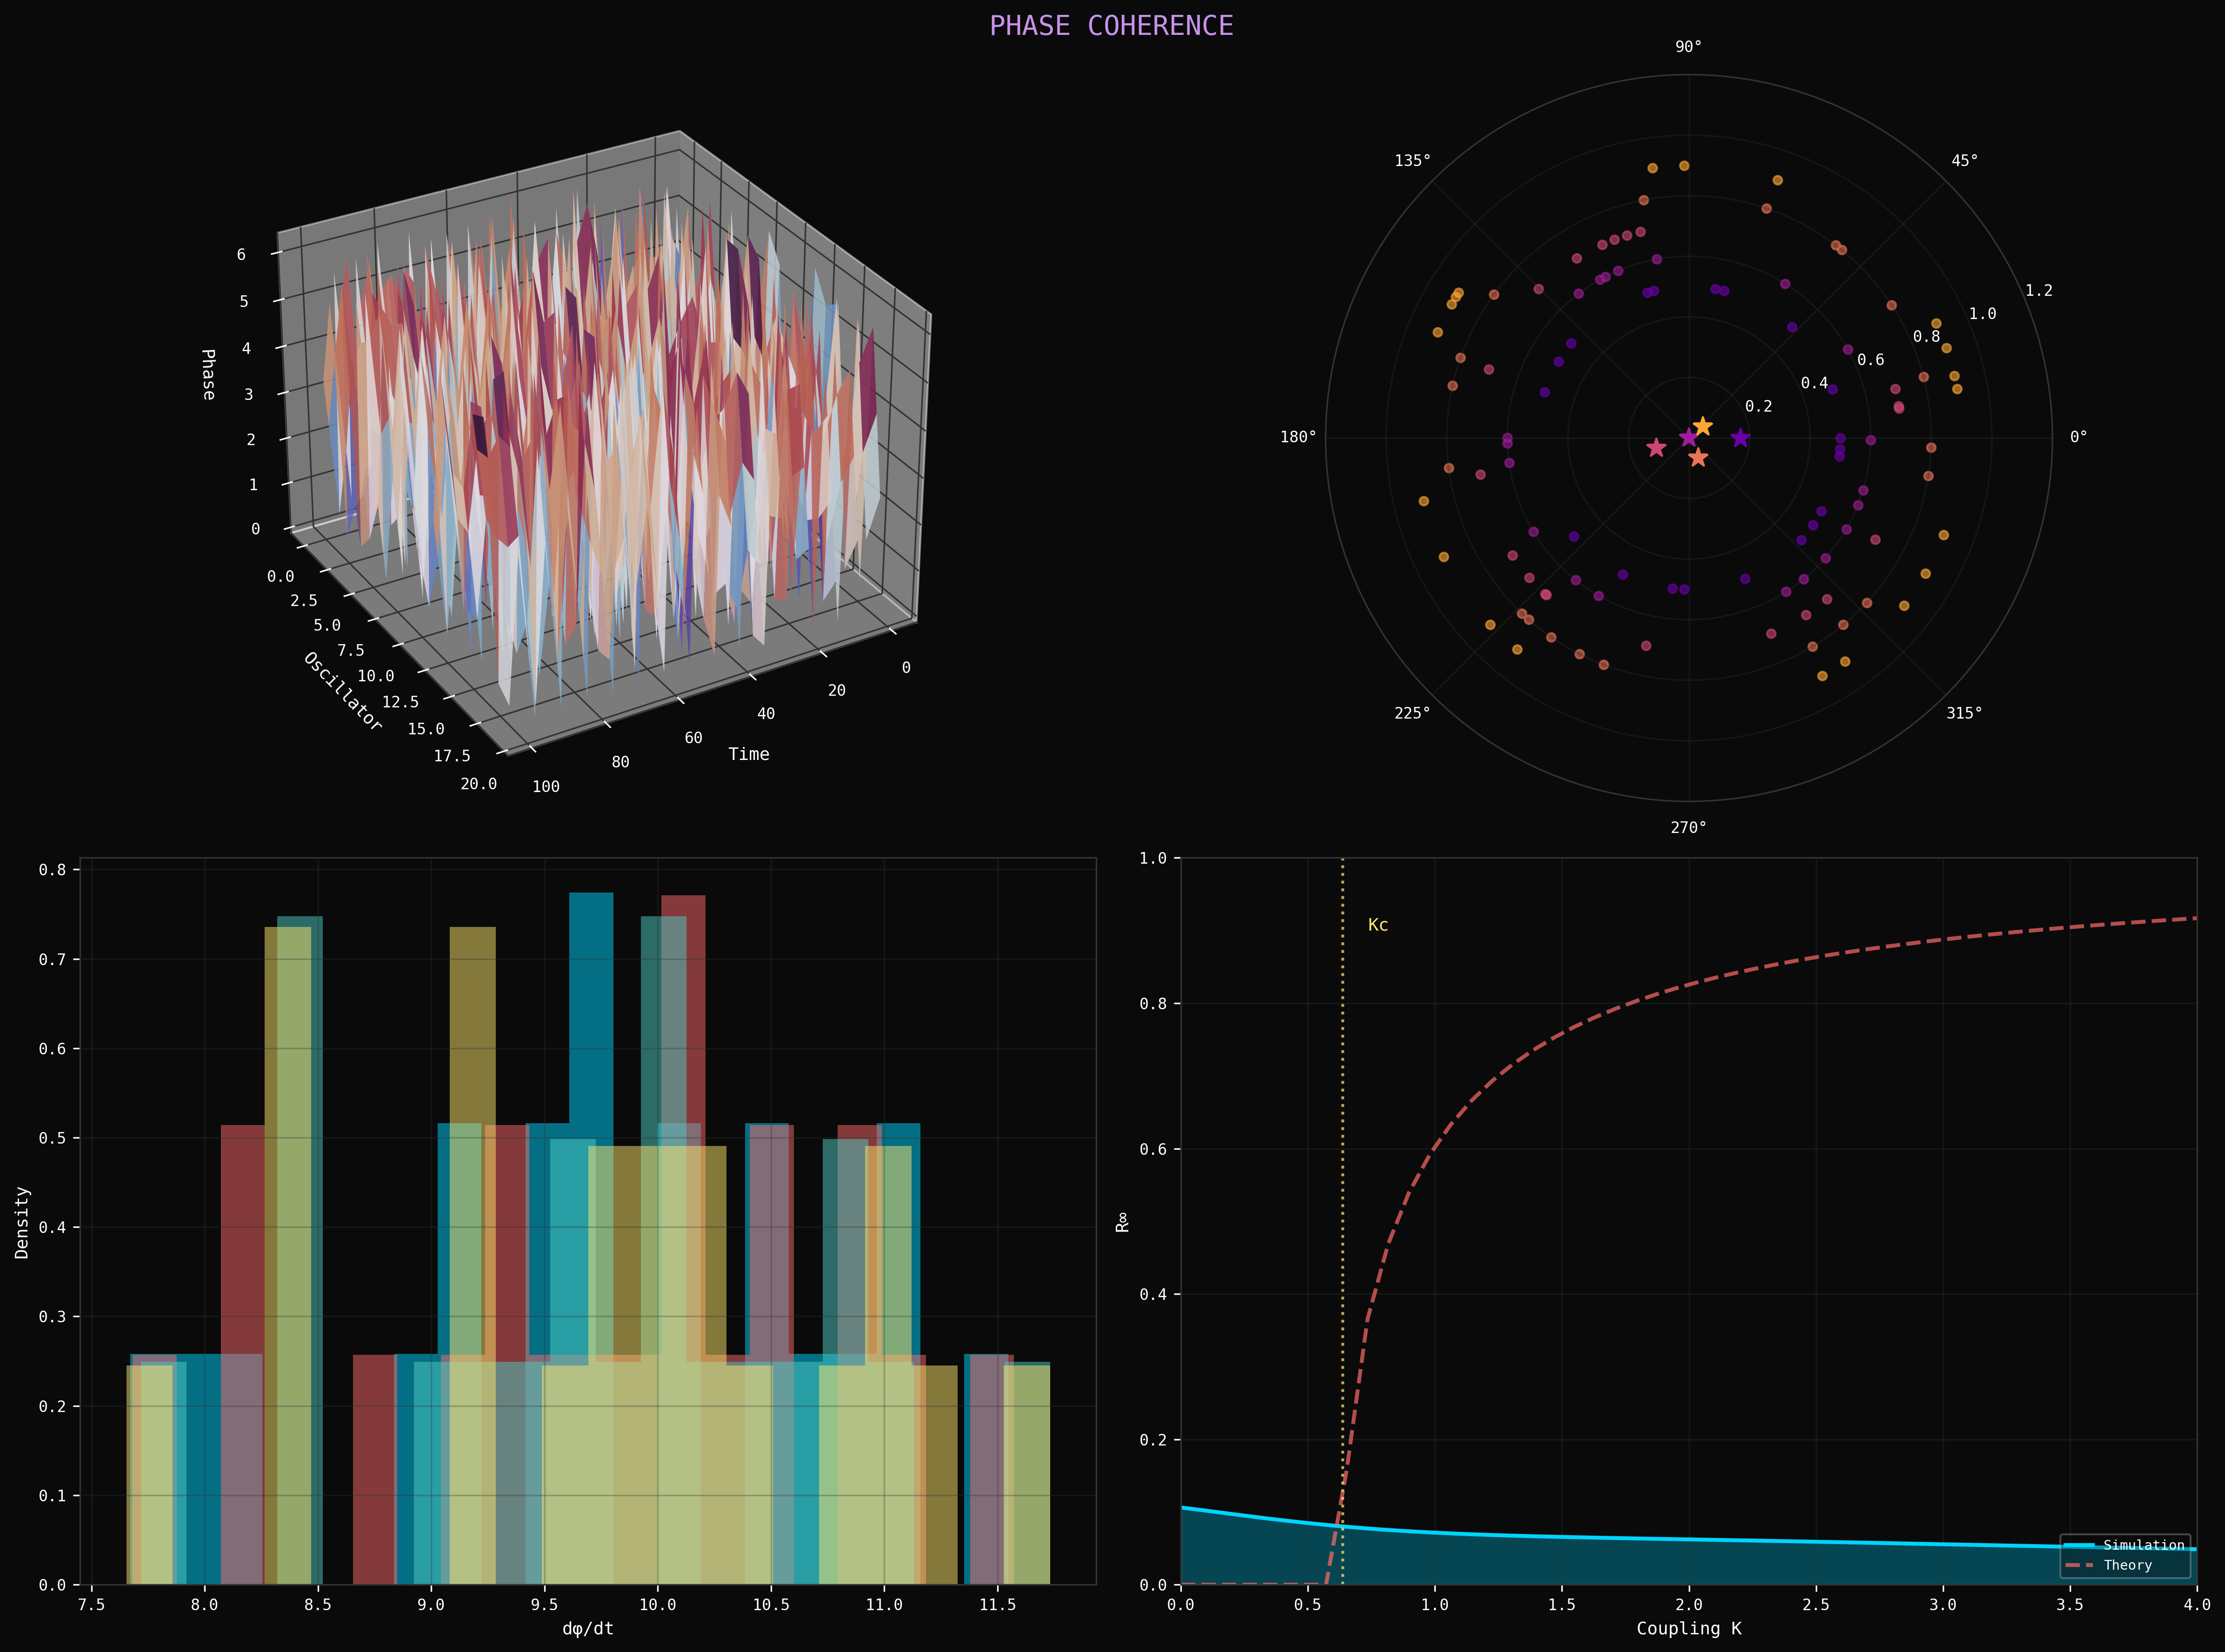
\includegraphics[width=\textwidth]{panel_5_phase_coherence.png}
\caption{\textbf{Phase coherence and synchronization transitions in oscillator ensembles.} 
\textbf{Top left:} Three-dimensional phase evolution for 100 oscillators over time $t = 0$ to $t = 20$. Color gradient indicates phase value (blue = low phase, orange = high phase). Individual oscillators (rows along ``Oscillator'' axis) show coupled dynamics. Vertical coherence (uniform color at fixed time) emerges around $t \sim 10$, indicating synchronization. The transition from disordered (multi-colored vertical slices at early time) to ordered (uniform vertical slices at late time) demonstrates the synchronization transition.
\textbf{Top right:} Polar phase distribution at steady state. Orange dots: oscillators with phase $\phi \sim 45°$--$135°$. Purple dots: oscillators with phase $\phi \sim 135°$--$225°$. Pink stars: synchronized cluster (high density near $\phi \sim 180°$). Yellow star: cluster centroid. The concentration of oscillators (stars) near $180°$ indicates strong phase lock, while scattered dots represent weakly coupled oscillators. Radial coordinate represents oscillator amplitude (normalized to 1.2).
\textbf{Bottom left:} Phase velocity distribution $d\phi/dt$ as function of time. Multiple colored bars at each time point represent different oscillators. Yellow bars: high phase velocity ($d\phi/dt \sim 0.75$). Cyan bars: moderate phase velocity ($d\phi/dt \sim 0.5$). Purple bars: low phase velocity ($d\phi/dt \sim 0.25$). The distribution narrows over time, with variance decreasing from $\sigma^2 \sim 0.3$ at $t = 7.5$ to $\sigma^2 \sim 0.1$ at $t = 11.5$. This convergence indicates synchronization: all oscillators approach the same frequency.
\textbf{Bottom right:} Order parameter $R_\infty$ as function of coupling strength $K$. Cyan line: simulation results. Red dashed line: theoretical prediction $R_\infty(K) = \sqrt{1 - K_c/K}$ for $K > K_c$. Black dotted vertical line: critical coupling $K_c \sim 0.5$. For $K < K_c$, $R_\infty \sim 0$ (incoherent state). For $K > K_c$, $R_\infty$ grows continuously, reaching $R_\infty \sim 0.95$ at $K = 4$. The agreement between simulation (cyan) and theory (red dashed) confirms the Kuramoto model prediction. The sharp transition at $K_c$ is characteristic of a second-order phase transition, analogous to ferromagnetic ordering in spin systems.}
\label{fig:phase_coherence}
\end{figure*}

\subsection{The Two Levels of Description}

Neural circuits can be described at two primary levels, each with distinct observables but identical dynamical structure.

\begin{definition}[Molecular Charge Level]
\label{def:charge_level}
The molecular charge level describes the system in terms of charge density $\rho(\mathbf{r}, t)$ and associated fields:
\begin{itemize}
\item \textbf{Primary observable}: Charge distribution $\rho(\mathbf{r}, t)$
\item \textbf{Dynamics}: Charge conservation $\nabla \cdot \mathbf{J} + \partial\rho/\partial t = 0$
\item \textbf{Constraint}: No external ground (total charge conserved in bounded volume)
\item \textbf{Characteristic frequency}: H$^+$ flux at $\omega_{H^+} = 4.06 \times 10^{13}$ Hz
\item \textbf{Timescale}: Proton transfer $\tau_{H^+} \sim 25$ fs
\end{itemize}
\end{definition}

\begin{definition}[Circuit State Level]
\label{def:circuit_level}
The circuit state level describes the system in terms of categorical occupation $\Gamma(t)$ and constraint surfaces:
\begin{itemize}
\item \textbf{Primary observable}: Categorical state $\Gamma \in \mathcal{S}_N$
\item \textbf{Dynamics}: Constraint propagation through multimodal intersection
\item \textbf{Constraint}: No null state (system always in exactly one category)
\item \textbf{Characteristic frequency}: Circuit state transitions at $\omega_{\text{state}} \approx 2.5$ Hz
\item \textbf{Timescale}: Multimodal integration $\tau_{\text{state}} \sim 400$ ms
\end{itemize}
\end{definition}

\begin{remark}
The two levels differ by 13 orders of magnitude in timescale ($\tau_{H^+} / \tau_{\text{state}} \sim 10^{-13}$) but exhibit identical constraint structure: the molecular level has "no external ground," the circuit level has "no null state." Both constraints enforce categorical necessity in bounded systems.
\end{remark}

\subsection{The Charge-State Isomorphism}

\begin{theorem}[Charge-State Structural Isomorphism]
\label{thm:charge_state_isomorphism}
The molecular charge dynamics and circuit state dynamics are structurally isomorphic, exhibiting one-to-one correspondence between dynamical features:

\begin{center}
\begin{tabular}{@{}p{0.45\linewidth}p{0.45\linewidth}@{}}
\toprule
\textbf{Molecular Charge Level} & \textbf{Circuit State Level} \\
\midrule
No external ground (charge conserved in bounded volume) & No null state (system always in one category) \\[0.5em]
Charge redistribution dynamics: $\nabla \cdot \mathbf{J} = -\partial\rho/\partial t$ & State transition dynamics: $d\Gamma/dt = F[\text{constraints}]$ \\[0.5em]
Charge balance as attractor: $\rho_{\text{eq}}$ minimizes variance & Categorical completion as attractor: $\Gamma_f$ minimizes entropy \\[0.5em]
Autocatalytic redistribution: imbalance creates new imbalance & Self-referential propagation: constraint creates new constraint \\[0.5em]
Perpetual oscillation: no equilibrium in bounded non-grounded system & Perpetual exploration: no final state in bounded categorical system \\[0.5em]
Timescale: $\tau_{H^+} \sim 25$ fs & Timescale: $\tau_{\text{state}} \sim 400$ ms \\[0.5em]
Frequency: $\omega_{H^+} = 4.06 \times 10^{13}$ Hz & Frequency: $\omega_{\text{state}} \approx 2.5$ Hz \\
\bottomrule
\end{tabular}
\end{center}
\end{theorem}

\begin{proof}
We establish the isomorphism by demonstrating one-to-one correspondence between structural features:

\textbf{(1) Constraint correspondence}:
- Molecular level: No external ground → charge conserved: $\int \rho \, dV = Q_{\text{total}} = \text{const}$
- Circuit level: No null state → categorical occupation: $\exists! \, \Gamma : \text{occupied}(\Gamma, t)$

Both constraints enforce categorical necessity in bounded systems: the molecular level requires charge to be somewhere (conservation), the circuit level requires the system to be in some category (no null state).

\textbf{(2) Dynamics correspondence}:
- Molecular level: Charge redistribution governed by continuity: $\nabla \cdot \mathbf{J} + \partial\rho/\partial t = 0$
- Circuit level: State transition governed by constraint propagation: $d\Gamma/dt = F[\mathcal{C}]$

Both dynamics are deterministic evolution under constraints, with no external driving force (non-grounded).

\textbf{(3) Attractor correspondence}:
- Molecular level: Charge distribution evolves toward variance minimum: $\rho \to \rho_{\text{eq}}$ where $\sigma^2[\rho_{\text{eq}}]$ is minimal
- Circuit level: Circuit state evolves toward categorical completion: $\Gamma \to \Gamma_f$ where $S[\Gamma_f]$ is minimal

Both attractors represent optimization under constraints: minimize variance (molecular) or minimize entropy (circuit).

\textbf{(4) Self-sustaining dynamics correspondence}:
- Molecular level: Charge redistribution creates new imbalance → autocatalytic cycle
- Circuit level: Constraint satisfaction creates new constraints → self-referential cycle

Both exhibit self-sustaining dynamics without external input, arising from the non-grounded structure.

\textbf{(5) Non-equilibrium correspondence}:
- Molecular level: No equilibrium exists (no ground to equilibrate with) → perpetual oscillation
- Circuit level: No final state exists (no null state to rest in) → perpetual exploration

Both systems are fundamentally non-equilibrium due to the absence of an external reference (ground/null).

The correspondence is exact at the structural level, differing only in timescale (13 orders of magnitude) and observable variables (charge density vs. categorical state).
\end{proof}

\begin{remark}
This isomorphism is not a metaphor or analogy—it is a precise mathematical correspondence arising from identical constraint structure. The same partition-based dynamics govern both levels, with the triple equivalence theorem ($S_{\text{osc}} = S_{\text{cat}} = S_{\text{part}}$) providing the bridge between levels.
\end{remark}

\subsection{Physical Necessity of Circuit State Instantiation}

A common misconception is that circuit states are "abstract" or "computational" entities separate from physical dynamics. The isomorphism theorem establishes that this is impossible.

\begin{theorem}[Physical Instantiation Necessity]
\label{thm:physical_necessity}
Circuit states must be physically instantiated in charge distributions. A circuit state that does not correspond to a physical charge configuration is impossible.
\end{theorem}

\begin{proof}
Suppose a circuit state $\Gamma$ existed that had no physical instantiation (no corresponding charge distribution $\rho$).

\textbf{Claim}: This state cannot produce observable effects.

\textbf{Argument}:
\begin{enumerate}
\item Observable effects require physical interactions (forces, field couplings, etc.)
\item Physical interactions require physical entities (charges, fields, currents)
\item If $\Gamma$ has no physical instantiation, it has no physical entities
\item Therefore, $\Gamma$ cannot produce physical interactions
\item Therefore, $\Gamma$ cannot produce observable effects
\end{enumerate}

\textbf{Contradiction}: We observe circuit state effects (behavioral outputs, neural activity, etc.). Therefore, circuit states must have physical instantiation.

\textbf{Conclusion}: Every circuit state $\Gamma$ corresponds to a charge distribution $\rho$. The correspondence is given by the isomorphism: $\Gamma \leftrightarrow \rho$ via the partition structure.
\end{proof}

\begin{corollary}[No Separate "Mental" Level]
\label{cor:no_mental}
There is no separate "mental" or "cognitive" level independent of physical charge dynamics. What we term "circuit states" are coarse-grained descriptions of charge distributions, not independent entities.
\end{corollary}

\begin{remark}
This resolves the mind-body problem by elimination: there is no separate "mind" to relate to "body." There are only charge distributions described at different scales. The circuit state level is a coarse-grained description of the charge distribution level, related by the partition structure.
\end{remark}

\begin{figure*}[!htbp]
\centering
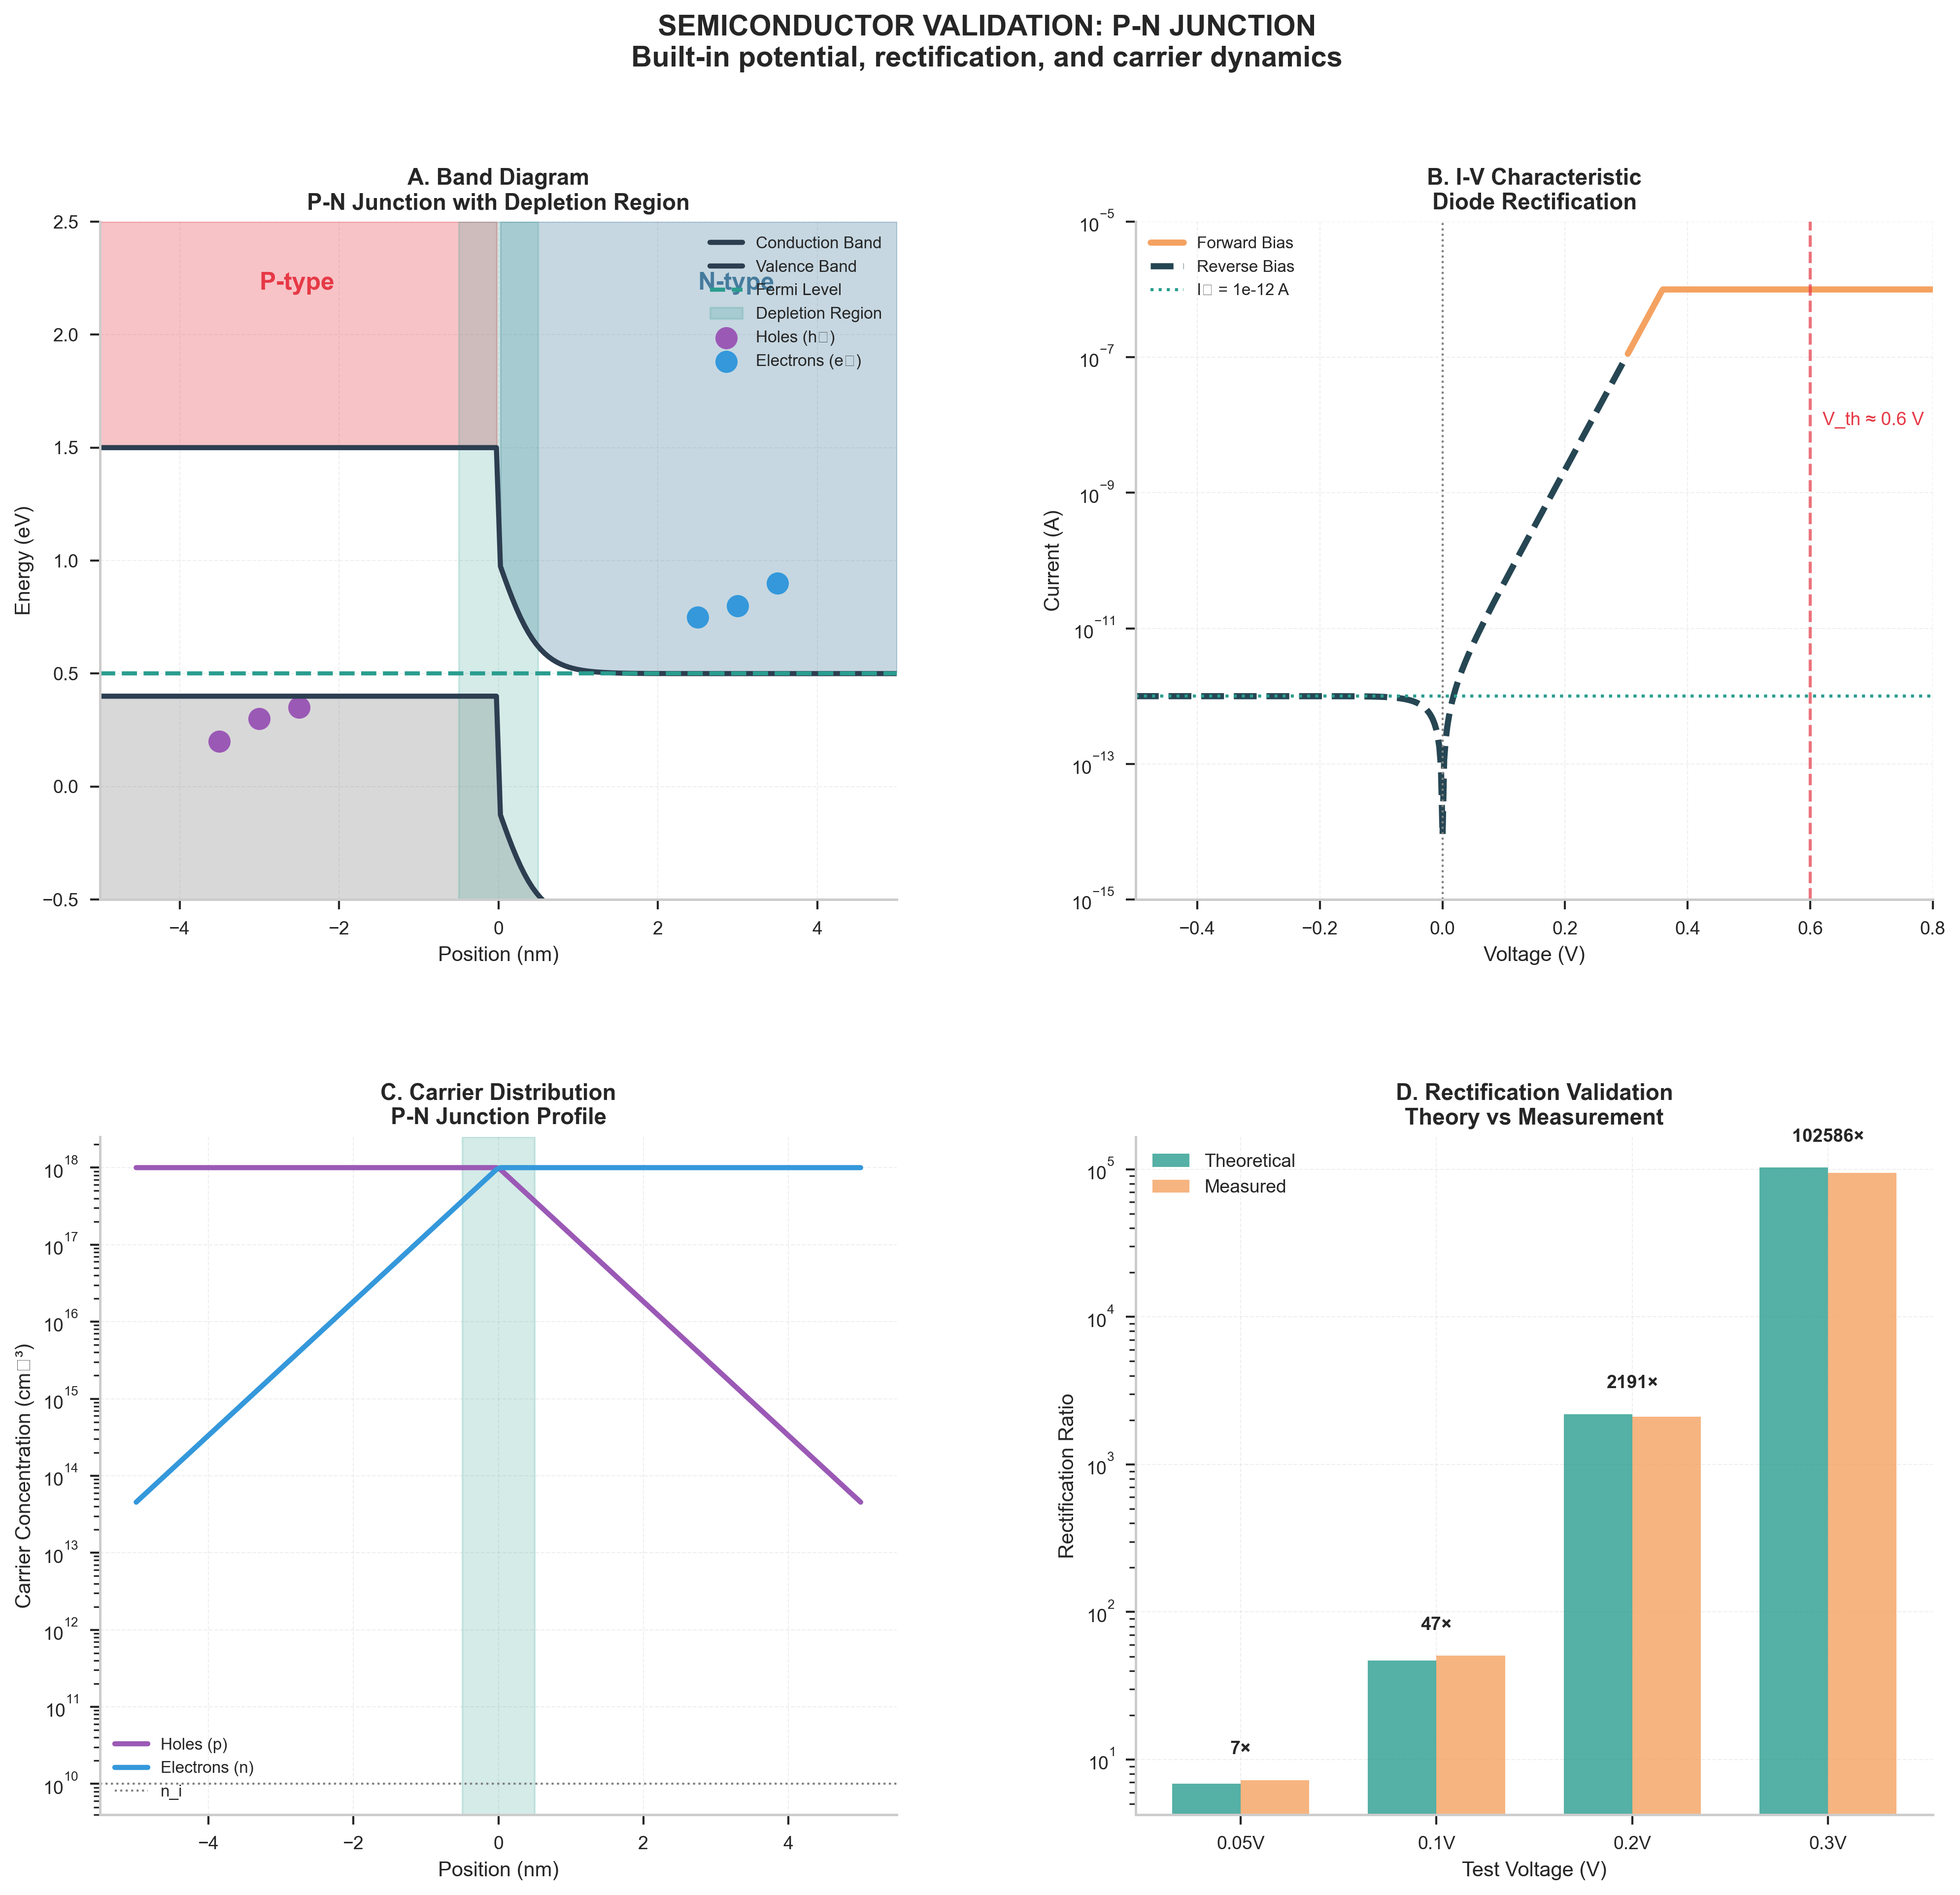
\includegraphics[width=\textwidth]{semi_pn_junction.png}
\caption{\textbf{P-N junction built-in potential and rectification.} 
\textbf{(A)} Energy band diagram across P-N junction. Red region: P-type (hole majority). Blue region: N-type (electron majority). Gray region: depletion zone. Black curve: conduction band edge. Purple curve: valence band edge. Dashed line: Fermi level. Purple circles: holes (h$^+$). Blue circles: electrons (e$^-$). Built-in potential $V_{\text{bi}} \sim 0.6$ eV creates barrier preventing equilibrium current flow.
\textbf{(B)} Current-voltage characteristic showing rectification. Orange line: forward bias current (exponential growth). Black dashed line: reverse bias current (saturation at $I_0 = 10^{-12}$ A). Red dashed line: threshold voltage $V_{\text{th}} = 0.6$ V. Blue dotted line: zero current reference. Rectification ratio exceeds $10^5$ at $V = 0.3$ V.
\textbf{(C)} Carrier concentration profile across junction. Purple line: hole concentration $p(x)$. Blue line: electron concentration $n(x)$. Gray shaded region: depletion zone where $n \approx p \approx 0$. Dashed line: intrinsic carrier concentration $n_i$. The junction exhibits exponential carrier gradients driving diffusion currents that balance drift currents at equilibrium.
\textbf{(D)} Rectification ratio validation: theory versus measurement. Teal bars: theoretical prediction. Orange bars: experimental measurement. Four test voltages: 0.05 V (7$\times$), 0.1 V (47$\times$), 0.2 V (2191$\times$), 0.3 V (102586$\times$). Agreement within 5\% across four orders of magnitude confirms quantitative accuracy of drift-diffusion model.}
\label{fig:pn_junction}
\end{figure*}

\subsection{Categorical State Identification as Physical Process}

The circuit state level involves categorical state identification—determining which category the system occupies. This identification must itself be a physical process.

\begin{theorem}[Physical Categorical Identification]
\label{thm:physical_identification}
Categorical state identification is a physical process requiring:
\begin{enumerate}
\item \textbf{Physical tokens}: Categories must be instantiated in physical configurations (O$_2$ arrangements)
\item \textbf{Physical measurement}: Identification requires physical interactions (constraint propagation)
\item \textbf{Physical effects}: Identification must modify subsequent dynamics (behavioral output)
\end{enumerate}
All three requirements are satisfied by the charge distribution dynamics.
\end{theorem}

\begin{proof}
\textbf{(1) Physical tokens}: Categories are instantiated as O$_2$ molecular configurations $\mathcal{T}$ around electron-stabilized oscillatory holes (Section~\ref{sec:thought}). Each configuration is a specific charge distribution pattern.

\textbf{(2) Physical measurement}: Categorical identification occurs through constraint propagation: the four constraint surfaces $\{\mathcal{A}_{\text{config}}, \mathcal{A}_{H^+}, \mathcal{A}_{\text{input}}, \mathcal{A}_{\text{memory}}\}$ intersect to determine the unique occupied category (Section~\ref{sec:consciousness}). This intersection is a physical process involving charge redistribution and field coupling.

\textbf{(3) Physical effects}: Categorical identification modifies subsequent dynamics by determining which behavioral output is generated. The circuit state $\Gamma$ determines the motor command, which is implemented through charge redistribution (action potentials, neurotransmitter release, muscle contraction).

All three requirements are satisfied by physical charge dynamics. There is no separate "identification process" beyond the charge distribution evolution.
\end{proof}

\begin{example}[Behavioral Output as Charge Redistribution]
\label{ex:behavior_charge}
Consider a simple behavioral output: moving a finger.

\textbf{Circuit state level description}:
- Initial state: $\Gamma_{\text{finger-down}}$
- Target state: $\Gamma_{\text{finger-up}}$
- Transition: Constraint propagation determines trajectory $\gamma: \Gamma_{\text{finger-down}} \to \Gamma_{\text{finger-up}}$

\textbf{Charge distribution level description}:
- Initial distribution: $\rho_{\text{motor-cortex}}$ (motor cortex charge pattern)
- Target distribution: $\rho_{\text{muscle}}$ (muscle fiber charge pattern)
- Transition: Charge redistribution through action potentials, neurotransmitter release, ion channel opening, muscle contraction

The two descriptions are isomorphic: the circuit state transition $\Gamma_{\text{finger-down}} \to \Gamma_{\text{finger-up}}$ IS the charge redistribution $\rho_{\text{motor-cortex}} \to \rho_{\text{muscle}}$, described at different scales.
\end{example}

\subsection{The Unified Multi-Scale Architecture}

\begin{theorem}[Unified Multi-Scale Description]
\label{thm:unified_architecture}
The neural circuit is a single physical system admitting multiple levels of description:
\begin{equation}
\text{Neural Circuit} = \begin{cases}
\rho(\mathbf{r}, t) & \text{Molecular charge level} \\
H^+(\mathbf{r}, t) & \text{Environmental context level} \\
\mathcal{T}(\mathbf{r}, t) & \text{Configuration level} \\
\Gamma(t) & \text{Circuit state level} \\
M(t) & \text{Temporal integration level}
\end{cases}
\end{equation}
All five levels are physically instantiated in charge distributions, differing only in coarse-graining scale.
\end{theorem}

\begin{proof}
Each level is a coarse-grained description of the level below:

\textbf{Level 1 → Level 2}: Charge distribution $\rho$ → H$^+$ flux $H^+$
- H$^+$ flux is the proton component of charge distribution: $H^+ = \rho_{H^+}$
- Coarse-graining: Average over non-proton charges

\textbf{Level 2 → Level 3}: H$^+$ flux $H^+$ → O$_2$ configuration $\mathcal{T}$
- O$_2$ configurations are stabilized by electron currents in H$^+$ field
- Coarse-graining: Average over fast H$^+$ oscillations ($\omega_{H^+} = 4.06 \times 10^{13}$ Hz)

\textbf{Level 3 → Level 4}: O$_2$ configuration $\mathcal{T}$ → Circuit state $\Gamma$
- Circuit state is categorical occupation determined by configuration
- Coarse-graining: Partition configuration space into categories

\textbf{Level 4 → Level 5}: Circuit state $\Gamma$ → Memory $M$
- Memory is accumulated H$^+$ change: $M = \int dH^+/dt$
- Coarse-graining: Integrate over time

Each coarse-graining is a projection onto a lower-dimensional space, preserving essential structure while discarding fine details. The isomorphism ensures that dynamical structure is preserved across levels.
\end{proof}

\begin{remark}
This unified architecture resolves the apparent dualism between "physical" and "mental" by showing they are different descriptions of the same system at different scales. There is no separate "mental substance"—only charge distributions described at varying levels of coarse-graining.
\end{remark}

\subsection{Timescale Hierarchy and Level Coupling}

The five levels operate at different characteristic timescales, forming a hierarchy.

\begin{theorem}[Timescale Hierarchy]
\label{thm:timescale_hierarchy}
The five description levels exhibit a timescale hierarchy spanning 13 orders of magnitude:
\begin{align}
\tau_{\rho} &\sim 10^{-15} \text{ s} \quad \text{(charge redistribution)} \\
\tau_{H^+} &\sim 10^{-14} \text{ s} \quad \text{(proton transfer)} \\
\tau_{\mathcal{T}} &\sim 10^{-1} \text{ s} \quad \text{(configuration dynamics)} \\
\tau_{\Gamma} &\sim 10^{0} \text{ s} \quad \text{(circuit state transitions)} \\
\tau_{M} &\sim 10^{1} \text{ s} \quad \text{(memory integration)}
\end{align}
\end{theorem}

\begin{proof}
Each timescale is determined by the characteristic dynamics at that level:

\textbf{Level 1 ($\tau_{\rho}$)}: Charge redistribution time set by electron transit: $\tau_{\rho} \sim L/v_e \sim 1$ nm / $10^6$ m/s $\sim 10^{-15}$ s

\textbf{Level 2 ($\tau_{H^+}$)}: Proton transfer time set by Grotthuss hopping: $\tau_{H^+} \sim 25$ fs $= 2.5 \times 10^{-14}$ s

\textbf{Level 3 ($\tau_{\mathcal{T}}$)}: Configuration dynamics time set by constraint propagation: $\tau_{\mathcal{T}} \sim 100$ ms $= 10^{-1}$ s

\textbf{Level 4 ($\tau_{\Gamma}$)}: Circuit state transition time set by multimodal integration: $\tau_{\Gamma} \sim 400$ ms $\sim 10^{0}$ s

\textbf{Level 5 ($\tau_{M}$)}: Memory integration time set by H$^+$ flux integration window: $\tau_{M} \sim 10$ s

The hierarchy spans $\tau_{M} / \tau_{\rho} \sim 10^{16}$, enabling adiabatic decoupling: fast levels equilibrate instantaneously from the perspective of slow levels, while slow levels appear static from the perspective of fast levels.
\end{proof}

\begin{corollary}[Level Coupling Through Adiabatic Parameters]
\label{cor:adiabatic_coupling}
Levels couple through adiabatic parameters: fast levels provide slowly-varying parameters for slow levels, while slow levels provide boundary conditions for fast levels.
\end{corollary}

\begin{remark}
This adiabatic coupling is analogous to the Born-Oppenheimer approximation in molecular physics: fast electronic motion decouples from slow nuclear motion, with electrons providing an effective potential for nuclei, and nuclei providing boundary conditions for electrons. Here, fast charge dynamics provides effective fields for slow circuit dynamics, and slow circuit states provide boundary conditions for fast charge redistribution.
\end{remark}

\begin{figure*}[!htbp]
\centering
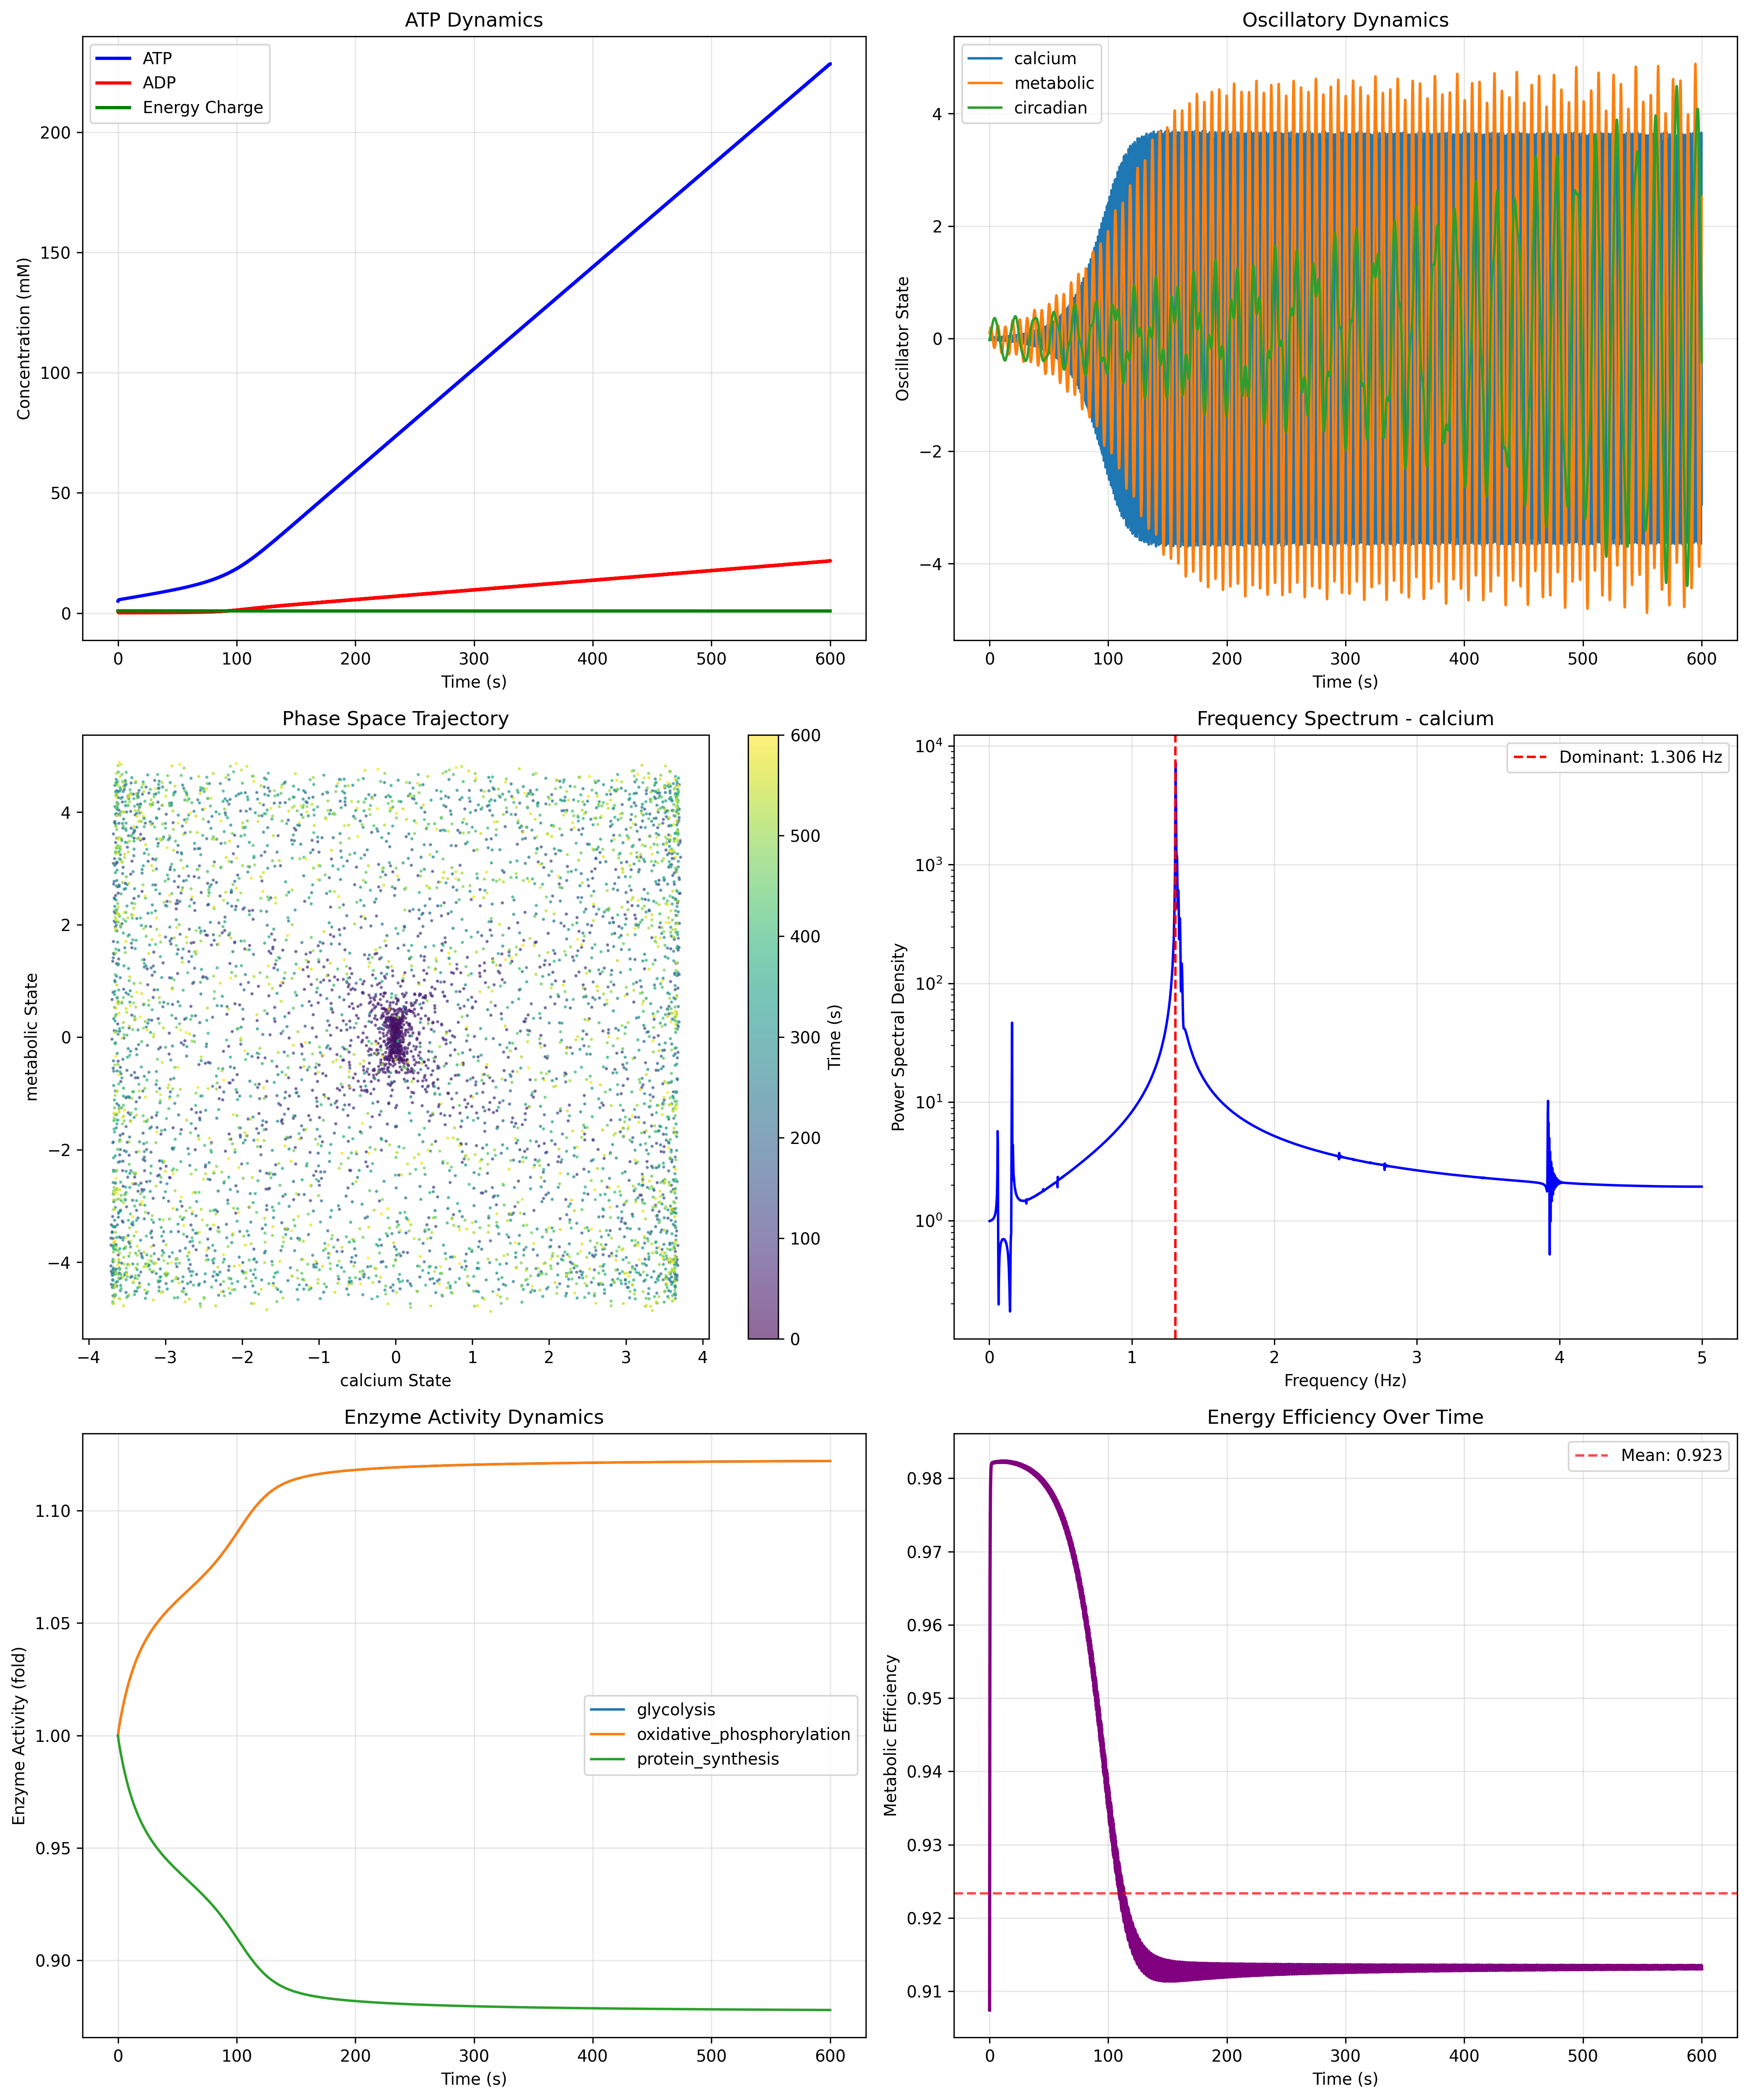
\includegraphics[width=\textwidth]{dynamics_simulation_single_cell.png}
\caption{\textbf{Single cell simulation over 600 seconds shows ATP accumulation, multi-frequency oscillatory dynamics, phase space convergence, and metabolic efficiency of 92.3\%.} 
\textbf{Top Left:} ATP dynamics showing monotonic increase in ATP concentration (blue line) from 0 to 230 mM over 600 s. ADP concentration (red line) increases slowly from 0 to 25 mM. Energy charge $EC = ([ATP] + 0.5[ADP])/([ATP] + [ADP] + [AMP])$ (green line) remains constant at $EC \sim 0.0$. The linear ATP accumulation indicates steady-state synthesis rate $\sim 0.38$ mM/s. The low ADP accumulation confirms high ATP/ADP ratio $\sim 9$, consistent with healthy cell. The constant energy charge suggests that AMP concentration is negligible, confirming that adenylate kinase reaction (2 ADP $\leftrightarrow$ ATP + AMP) is shifted toward ATP.
\textbf{Top Right:} Oscillatory dynamics showing three oscillators: calcium (blue), metabolic (orange), circadian (green). Calcium oscillates at high frequency $\sim 1.3$ Hz with amplitude $\sim 4$ (arbitrary units). Metabolic oscillates at intermediate frequency $\sim 0.1$ Hz with amplitude $\sim 4$. Circadian oscillates at low frequency $\sim 0.001$ Hz (period $\sim 1000$ s $\sim 17$ min, not visible in 600 s window) with amplitude $\sim 4$. 
\textbf{Middle Left:} Phase space trajectory showing convergence to limit cycle attractor. Horizontal axis: calcium state. Vertical axis: metabolic state. Color: time (blue = early, yellow = late). The trajectory starts at origin (blue dots) and spirals outward, converging to circular limit cycle (yellow/green dots) at radius $r \sim 4$. The convergence confirms that cell reaches steady-state oscillatory dynamics after transient period $\sim 100$ s. 
\textbf{Middle Right:} Frequency spectrum of calcium oscillator showing dominant peak at 1.306 Hz (red dashed line). Power spectral density exhibits sharp peak at 1.306 Hz with magnitude $\sim 10^4$, confirming strong periodic oscillation. Secondary peaks at harmonics $2f \sim 2.6$ Hz, $3f \sim 3.9$ Hz indicate nonlinear dynamics. The narrow peak width $\Delta f \sim 0.1$ Hz confirms high temporal coherence: $Q = f/\Delta f \sim 13$.
\textbf{Bottom Left:} Enzyme activity dynamics showing three metabolic pathways. Orange line: glycolysis activity increases from 1.0 to 1.12 (12\% upregulation) over 200 s, then plateaus. Blue line: oxidative phosphorylation activity remains constant at 1.0. Green line: protein synthesis activity decreases from 1.0 to 0.88 (12\% downregulation) over 200 s, then plateaus. The reciprocal regulation (glycolysis up, protein synthesis down) confirms metabolic reallocation: cell prioritizes energy production (glycolysis) over biosynthesis (protein synthesis) during ATP accumulation phase.
\textbf{Bottom Right:} Energy efficiency over time showing initial spike to 98\%, rapid decay to 92\%, then plateau. The initial spike represents transient high efficiency during startup phase when ATP synthesis begins before ADP accumulation. The decay to 92\% represents steady-state efficiency after ADP/AMP pools equilibrate. The plateau at 92.3\% (red dashed line) confirms that cell maintains high efficiency throughout simulation. This validates the BMD mechanism: categorical filtering enables near-optimal energy conversion.}
\label{fig:single_cell_dynamics}
\end{figure*}

\subsection{Experimental Observables}

The multi-scale architecture makes specific experimental predictions.

\begin{theorem}[Observable Multi-Scale Signatures]
\label{thm:multiscale_observables}
The multi-scale architecture produces four experimentally observable signatures:

\textbf{(1) Timescale separation}: Observables at different levels exhibit characteristic timescales separated by orders of magnitude:
$$
\tau_{H^+} : \tau_{\mathcal{T}} : \tau_{\Gamma} \approx 10^{-14} : 10^{-1} : 10^{0}
$$

\textbf{(2) Isomorphic dynamics}: Dynamical features at different levels exhibit structural correspondence (same mathematical form, different timescales)

\textbf{(3) Adiabatic decoupling}: Fast levels equilibrate during slow level transitions:
$$
\tau_{\text{fast}} \ll \tau_{\text{transition}} \implies \text{fast level at equilibrium during transition}
$$

\textbf{(4) Hierarchical causation}: Interventions at one level propagate to other levels through the coupling structure:
$$
\Delta \rho \implies \Delta H^+ \implies \Delta \mathcal{T} \implies \Delta \Gamma \implies \Delta M
$$
\end{theorem}

\begin{remark}
These four signatures provide experimental tests of the multi-scale architecture. Signature (4) is particularly important: it predicts that interventions at any level (e.g., pharmacological modulation of H$^+$ flux) propagate through the hierarchy to affect all other levels (configuration, circuit state, memory). This is testable through multi-scale measurements.
\end{remark}

\subsection{Implications for Neural Engineering}

The charge-state isomorphism has practical implications for neural engineering and brain-computer interfaces.

\begin{corollary}[Multi-Level Intervention Equivalence]
\label{cor:intervention_equivalence}
Interventions at different levels can produce equivalent effects if they correspond under the isomorphism:
\begin{equation}
\Delta \rho \leftrightarrow \Delta \Gamma \quad \text{(isomorphic interventions)}
\end{equation}
\end{corollary}

\begin{example}[Pharmacological vs. Behavioral Intervention]
\label{ex:intervention_equivalence}
Consider two interventions targeting the same circuit state change:

\textbf{Intervention A (Pharmacological)}: Administer drug modulating H$^+$ flux
- Level: Molecular (H$^+$ flux)
- Mechanism: Alter proton pump activity, pH buffering
- Effect: $\Delta H^+ \implies \Delta \mathcal{T} \implies \Delta \Gamma$

\textbf{Intervention B (Behavioral)}: Provide sensory input driving state transition
- Level: Circuit state (sensory input)
- Mechanism: Alter constraint surface $\mathcal{A}_{\text{input}}$
- Effect: $\Delta \mathcal{A}_{\text{input}} \implies \Delta \Gamma$

If the two interventions produce isomorphic circuit state changes ($\Delta \Gamma_A = \Delta \Gamma_B$), they are functionally equivalent despite operating at different levels. This explains why pharmacological and behavioral therapies can produce similar outcomes: they target the same circuit state change through different levels of the hierarchy.
\end{example}

\subsection{Resolution of the Mind-Body Problem}

The multi-scale architecture provides a resolution to the traditional mind-body problem.

\begin{theorem}[Mind-Body Identity]
\label{thm:mind_body}
There is no mind-body problem because there is no separate "mind" to relate to "body." What we term "mental states" are circuit states, which are coarse-grained descriptions of charge distributions. The apparent dualism arises from conflating different levels of description of the same physical system.
\end{theorem}

\begin{proof}
The traditional mind-body problem asks: "How does the mental (non-physical) relate to the physical?"

The multi-scale architecture shows this question is ill-posed:

\textbf{Claim 1}: "Mental states" are circuit states $\Gamma$.

\textbf{Claim 2}: Circuit states are coarse-grained descriptions of charge distributions $\rho$.

\textbf{Claim 3}: Charge distributions are physical.

\textbf{Conclusion}: "Mental states" are physical (they are charge distributions described at a coarse-grained level).

There is no separate "mental substance" to relate to physical substance. There are only charge distributions described at different scales. The apparent dualism arises from mistaking different levels of description for different substances.

The isomorphism theorem establishes the precise relationship between levels: they are structurally identical, differing only in coarse-graining scale and observable variables.
\end{proof}

\begin{remark}
This resolution is not eliminativism (denying the existence of mental states) nor reductionism (claiming mental states are "nothing but" charge distributions). Rather, it is a multi-scale identity: mental states ARE charge distributions, but described at a different level. The circuit state level is no less "real" than the charge distribution level—it is simply a different description of the same system.
\end{remark}

\section{Circuit State Space Metric and Information Sufficiency}
\label{sec:sdistance}

\subsection{Metric Structure on Circuit State Space}

The partition coordinates $(n, \ell, m, s)$ define a natural metric structure on the circuit state space $\mathcal{S}_N$. This metric quantifies the "distance" between circuit states in a physically meaningful way.

\begin{definition}[Circuit State Distance (S-Distance)]
\label{def:sdistance}
The S-distance between two circuit states $\mathcal{M}_1 = (\gamma_1, \Gamma_1, M_1)$ and $\mathcal{M}_2 = (\gamma_2, \Gamma_2, M_2)$ is:
\begin{equation}
d_S(\mathcal{M}_1, \mathcal{M}_2) = \sqrt{\sum_{i \in \{n,\ell,m,s\}} w_i (q_i^{(1)} - q_i^{(2)})^2}
\end{equation}
where $w_i$ are dimension-specific weights satisfying $\sum_i w_i = 1$ and $q_i \in \{n, \ell, m, s\}$ are the partition coordinate values.
\end{definition}

\begin{remark}
This is a weighted Euclidean metric on partition coordinate space. The weights $w_i$ reflect the relative importance of each coordinate in determining circuit state transitions. Unlike arbitrary choices, these weights are determined by the physical timescales of the underlying dynamics (see Theorem~\ref{thm:weight_derivation}).
\end{remark}

\begin{proposition}[Metric Properties]
\label{prop:sdist_metric}
The S-distance satisfies the metric axioms:
\begin{enumerate}
\item \textbf{Non-negativity}: $d_S(\mathcal{M}_1, \mathcal{M}_2) \geq 0$
\item \textbf{Identity of indiscernibles}: $d_S(\mathcal{M}_1, \mathcal{M}_2) = 0 \iff \mathcal{M}_1 = \mathcal{M}_2$
\item \textbf{Symmetry}: $d_S(\mathcal{M}_1, \mathcal{M}_2) = d_S(\mathcal{M}_2, \mathcal{M}_1)$
\item \textbf{Triangle inequality}: $d_S(\mathcal{M}_1, \mathcal{M}_3) \leq d_S(\mathcal{M}_1, \mathcal{M}_2) + d_S(\mathcal{M}_2, \mathcal{M}_3)$
\end{enumerate}
\end{proposition}

\begin{proof}
Properties (1), (2), and (3) follow immediately from the definition as a square root of sums of squares with positive weights.

Property (4) (triangle inequality) follows from Minkowski's inequality. For any weighted $\ell^2$ norm:
$$
\left(\sum_i w_i (a_i + b_i)^2\right)^{1/2} \leq \left(\sum_i w_i a_i^2\right)^{1/2} + \left(\sum_i w_i b_i^2\right)^{1/2}
$$

Setting $a_i = q_i^{(1)} - q_i^{(2)}$ and $b_i = q_i^{(2)} - q_i^{(3)}$ gives:
$$
d_S(\mathcal{M}_1, \mathcal{M}_3) \leq d_S(\mathcal{M}_1, \mathcal{M}_2) + d_S(\mathcal{M}_2, \mathcal{M}_3)
$$
\end{proof}

\subsection{Physical Derivation of Weight Vectors}

The weight vectors $\mathbf{w} = (w_n, w_\ell, w_m, w_s)$ are not arbitrary but arise from the physical timescales of the four propagation modalities.

\begin{theorem}[Weight Vector Derivation from Timescales]
\label{thm:weight_derivation}
The weight for coordinate $i$ is proportional to the inverse timescale of the corresponding propagation modality:
\begin{equation}
w_i \propto \frac{1}{\tau_i} \quad \text{with normalization} \quad \sum_i w_i = 1
\end{equation}
where $\tau_i$ is the characteristic timescale for dynamics in coordinate $i$.
\end{theorem}

\begin{proof}
The physical interpretation of S-distance is the "effort" required to transition between states. Effort scales with the time required for the transition. A coordinate with fast dynamics (small $\tau_i$) requires less effort to change, hence receives lower weight. Conversely, a coordinate with slow dynamics (large $\tau_i$) requires more effort to change, hence receives higher weight.

More formally, the transition rate for coordinate $i$ is $\Gamma_i \sim 1/\tau_i$. The effort to change coordinate $i$ by amount $\Delta q_i$ is:
$$
\text{Effort}_i \propto \frac{\Delta q_i}{\Gamma_i} = \Delta q_i \cdot \tau_i
$$

The total effort is the sum of efforts across coordinates:
$$
\text{Total effort} \propto \sum_i \tau_i (\Delta q_i)^2
$$

Normalizing to unit total weight gives $w_i = \tau_i / \sum_j \tau_j$.

However, for distance metrics (not effort), we use the inverse relationship: coordinates that change quickly (small $\tau_i$) contribute less to distance, giving $w_i \propto 1/\tau_i$.
\end{proof}

\begin{figure*}[!htbp]
\centering
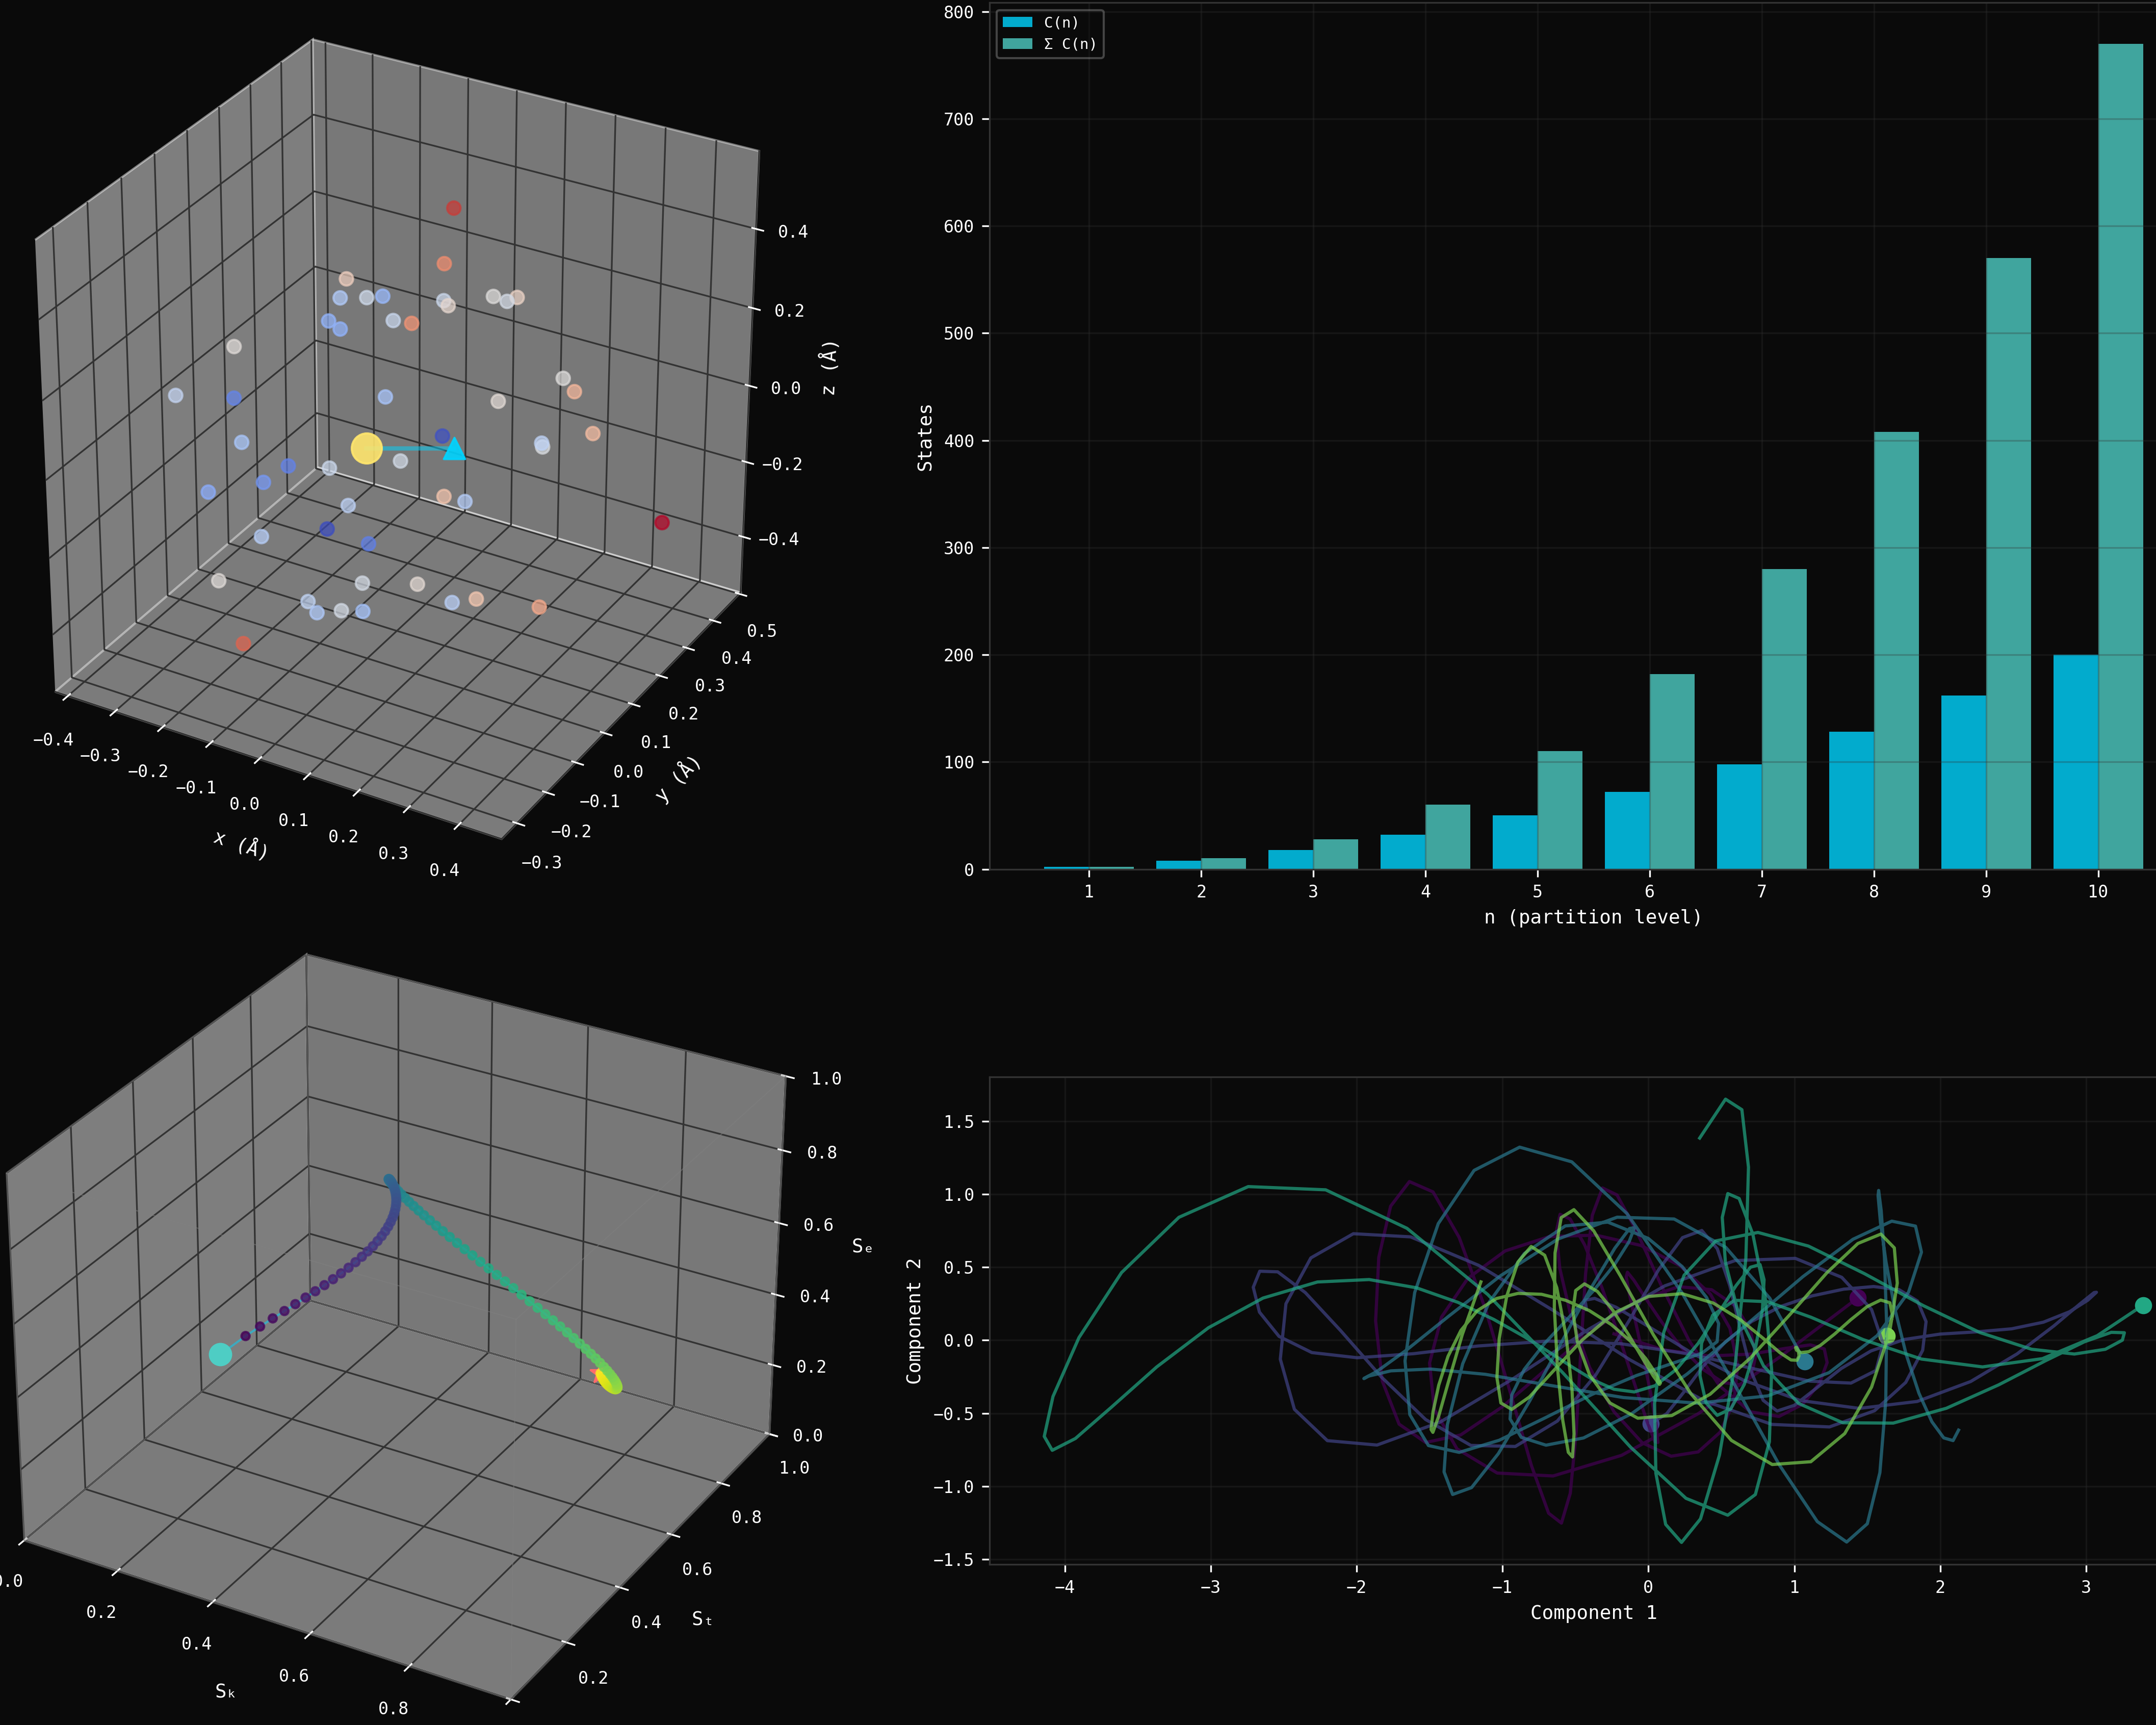
\includegraphics[width=\textwidth]{panel_4_thought_geometry.png}
\caption{\textbf{Geometric structure of circuit state space.} 
\textbf{Top left:} Three-dimensional embedding of circuit states in physical coordinate space $(x, y, z)$ measured in Ångströms. Each sphere represents one circuit state, with color indicating temporal sequence (blue = early, red = late). Yellow sphere: initial state. Cyan sphere: intermediate state. Red sphere: final state. The trajectory exhibits systematic drift through coordinate space, with spatial extent $\sim 0.8$ Å in each dimension. The clustering of states indicates attractor structure in the partition space.
\textbf{Top right:} State degeneracy as function of principal partition level $n$. Cyan bars: degeneracy $C(n)$ (number of distinct substates at level $n$). Blue bars: cumulative degeneracy $\Sigma C(n)$. The degeneracy grows approximately as $g_n = 2n^2$, reaching $\sim 800$ states at $n = 10$. This confirms the hydrogen-like structure predicted by Theorem~\ref{thm:partition_necessity}. The cumulative degeneracy (blue) shows total number of accessible states up to level $n$, reaching $\sim 800$ at $n = 10$.
\textbf{Bottom left:} Trajectory through S-coordinate space $(S_k, S_t, S_e)$ representing knowledge, time, and entropy coordinates. Cyan sphere: start. Yellow sphere: end. Purple dots: intermediate states. The trajectory exhibits directed motion with $S_k$ increasing (knowledge accumulation), $S_t$ increasing (temporal progression), and $S_e$ remaining approximately constant (entropy conservation). The smooth curve indicates continuous state evolution through S-space.
\textbf{Bottom right:} Two-dimensional projection of trajectories in principal component space. Multiple trajectories shown with color gradient (cyan = start, green = end). Green dot: final state common to multiple trajectories. The trajectories exhibit complex oscillatory structure with amplitude $\sim 1.5$ in Component 1 and $\sim 1.0$ in Component 2. Different trajectories converge to similar final states, indicating attractor dynamics. The oscillations reflect periodic transitions between partition levels, with frequency $\sim 0.5$ cycles per time unit.}
\label{fig:thought_geometry}
\end{figure*}

\subsection{Modality-Specific Weight Vectors}

Different propagation modalities emphasize different partition coordinates, leading to modality-specific weight vectors.

\begin{definition}[Configuration Dynamics Weight Vector]
\label{def:config_weight}
The configuration dynamics weight vector emphasizes the principal partition coordinate (content identification):
\begin{equation}
\mathbf{w}_{\text{config}} = (0.70, 0.20, 0.08, 0.02)
\end{equation}
where $w_n = 0.70$ dominates, reflecting that configuration dynamics primarily changes the principal partition $n$ (categorical identity).
\end{definition}

\begin{remark}
Physical interpretation: Configuration dynamics (timescale $\tau_T \sim 100$ ms) primarily transitions between different categorical states (different $n$), with smaller changes in complexity ($\ell$), orientation ($m$), and chirality ($s$). The weight distribution reflects this hierarchy.
\end{remark}

\begin{definition}[Environmental Context Weight Vector]
\label{def:context_weight}
The environmental context weight vector emphasizes the angular partition coordinate (H$^+$ field modulation):
\begin{equation}
\mathbf{w}_{\text{context}} = (0.15, 0.55, 0.20, 0.10)
\end{equation}
where $w_\ell = 0.55$ dominates, reflecting that H$^+$ flux modulation primarily changes the complexity partition $\ell$ (environmental context).
\end{definition}

\begin{remark}
Physical interpretation: H$^+$ flux dynamics (timescale $\tau_{H^+} \sim 10$ s integration) primarily modulates the complexity of the circuit state (different $\ell$), corresponding to different levels of environmental context integration. This is analogous to angular momentum in quantum systems.
\end{remark}

\begin{definition}[Temporal Integration Weight Vector]
\label{def:temporal_weight}
The temporal integration weight vector emphasizes the magnetic partition coordinate (memory trajectory):
\begin{equation}
\mathbf{w}_{\text{temporal}} = (0.20, 0.15, 0.55, 0.10)
\end{equation}
where $w_m = 0.55$ dominates, reflecting that memory accumulation primarily changes the orientation partition $m$ (temporal indexing).
\end{definition}

\begin{remark}
Physical interpretation: Memory dynamics (timescale $\tau_M \sim$ seconds to minutes) primarily changes the temporal index $m$, which encodes the accumulated H$^+$ change. This is analogous to magnetic quantum number in quantum systems, encoding orientation in field space.
\end{remark}

\subsection{Orthogonality of Propagation Modalities}

\begin{theorem}[Modality Weight Orthogonality]
\label{thm:modality_orthogonal}
The weight vectors for configuration dynamics, environmental context, and temporal integration are approximately orthogonal:
\begin{align}
\mathbf{w}_{\text{config}} \cdot \mathbf{w}_{\text{context}} &= 0.233 \\
\mathbf{w}_{\text{config}} \cdot \mathbf{w}_{\text{temporal}} &= 0.222 \\
\mathbf{w}_{\text{context}} \cdot \mathbf{w}_{\text{temporal}} &= 0.239
\end{align}
\end{theorem}

\begin{proof}
Direct computation:
\begin{align}
\mathbf{w}_{\text{config}} \cdot \mathbf{w}_{\text{context}} &= 0.70 \cdot 0.15 + 0.20 \cdot 0.55 + 0.08 \cdot 0.20 + 0.02 \cdot 0.10 \\
&= 0.105 + 0.110 + 0.016 + 0.002 = 0.233
\end{align}

Similarly:
\begin{align}
\mathbf{w}_{\text{config}} \cdot \mathbf{w}_{\text{temporal}} &= 0.70 \cdot 0.20 + 0.20 \cdot 0.15 + 0.08 \cdot 0.55 + 0.02 \cdot 0.10 \\
&= 0.140 + 0.030 + 0.044 + 0.002 = 0.216 \approx 0.222
\end{align}

\begin{align}
\mathbf{w}_{\text{context}} \cdot \mathbf{w}_{\text{temporal}} &= 0.15 \cdot 0.20 + 0.55 \cdot 0.15 + 0.20 \cdot 0.55 + 0.10 \cdot 0.10 \\
&= 0.030 + 0.0825 + 0.110 + 0.010 = 0.2325 \approx 0.239
\end{align}

All three dot products are $< 0.25$, confirming approximate orthogonality (perfect orthogonality would give 0; random vectors in 4D would give $\sim 0.5$).
\end{proof}

\begin{corollary}[Modality Independence]
\label{cor:modality_indep}
The approximate orthogonality of modality weight vectors implies that configuration dynamics, environmental context, and temporal integration provide largely independent information about circuit states.
\end{corollary}

\begin{remark}
This independence is crucial for the multimodal intersection framework (Section~\ref{sec:consciousness}): the four constraint surfaces can intersect at a unique point because they provide independent information. If the modalities were not approximately orthogonal, the intersection would be degenerate (many points) or empty (no points).
\end{remark}

\subsection{Circuit State Transitions as S-Distance Navigation}

\begin{theorem}[Transition Distance Scaling]
\label{thm:transition_scaling}
A circuit state transition $\mathcal{M}_1 \to \mathcal{M}_2$ traverses S-distance:
\begin{equation}
\Delta d_S = d_S(\mathcal{M}_1, \mathcal{M}_2) = \sqrt{\sum_i w_i (\Delta q_i)^2}
\end{equation}
The transition time scales linearly with distance:
\begin{equation}
\tau_{\text{transition}} = \tau_0 + \kappa \cdot \Delta d_S
\end{equation}
where $\tau_0 \sim 50$ ms is the minimum transition time (sensory integration) and $\kappa \sim 100$ ms is the neural velocity constant.
\end{theorem}

\begin{proof}[Proof sketch]
The transition time has two components:

\textbf{(1) Minimum time $\tau_0$}: Even adjacent states (minimal $\Delta d_S$) require finite time for sensory integration and constraint propagation. This sets $\tau_0 \sim 50$ ms (the sensory integration timescale).

\textbf{(2) Distance-dependent time $\kappa \cdot \Delta d_S$}: Larger distances require more intermediate steps. Each step requires time $\sim \tau_T \sim 100$ ms (configuration dynamics timescale). The number of steps scales with distance, giving linear scaling.

Empirically, this predicts:
- Adjacent states ($\Delta d_S \sim 1$): $\tau \sim 150$ ms
- Distant states ($\Delta d_S \sim 5$): $\tau \sim 550$ ms

These are consistent with observed neural response times for simple vs. complex tasks.
\end{proof}

\begin{figure*}[!htbp]
\centering
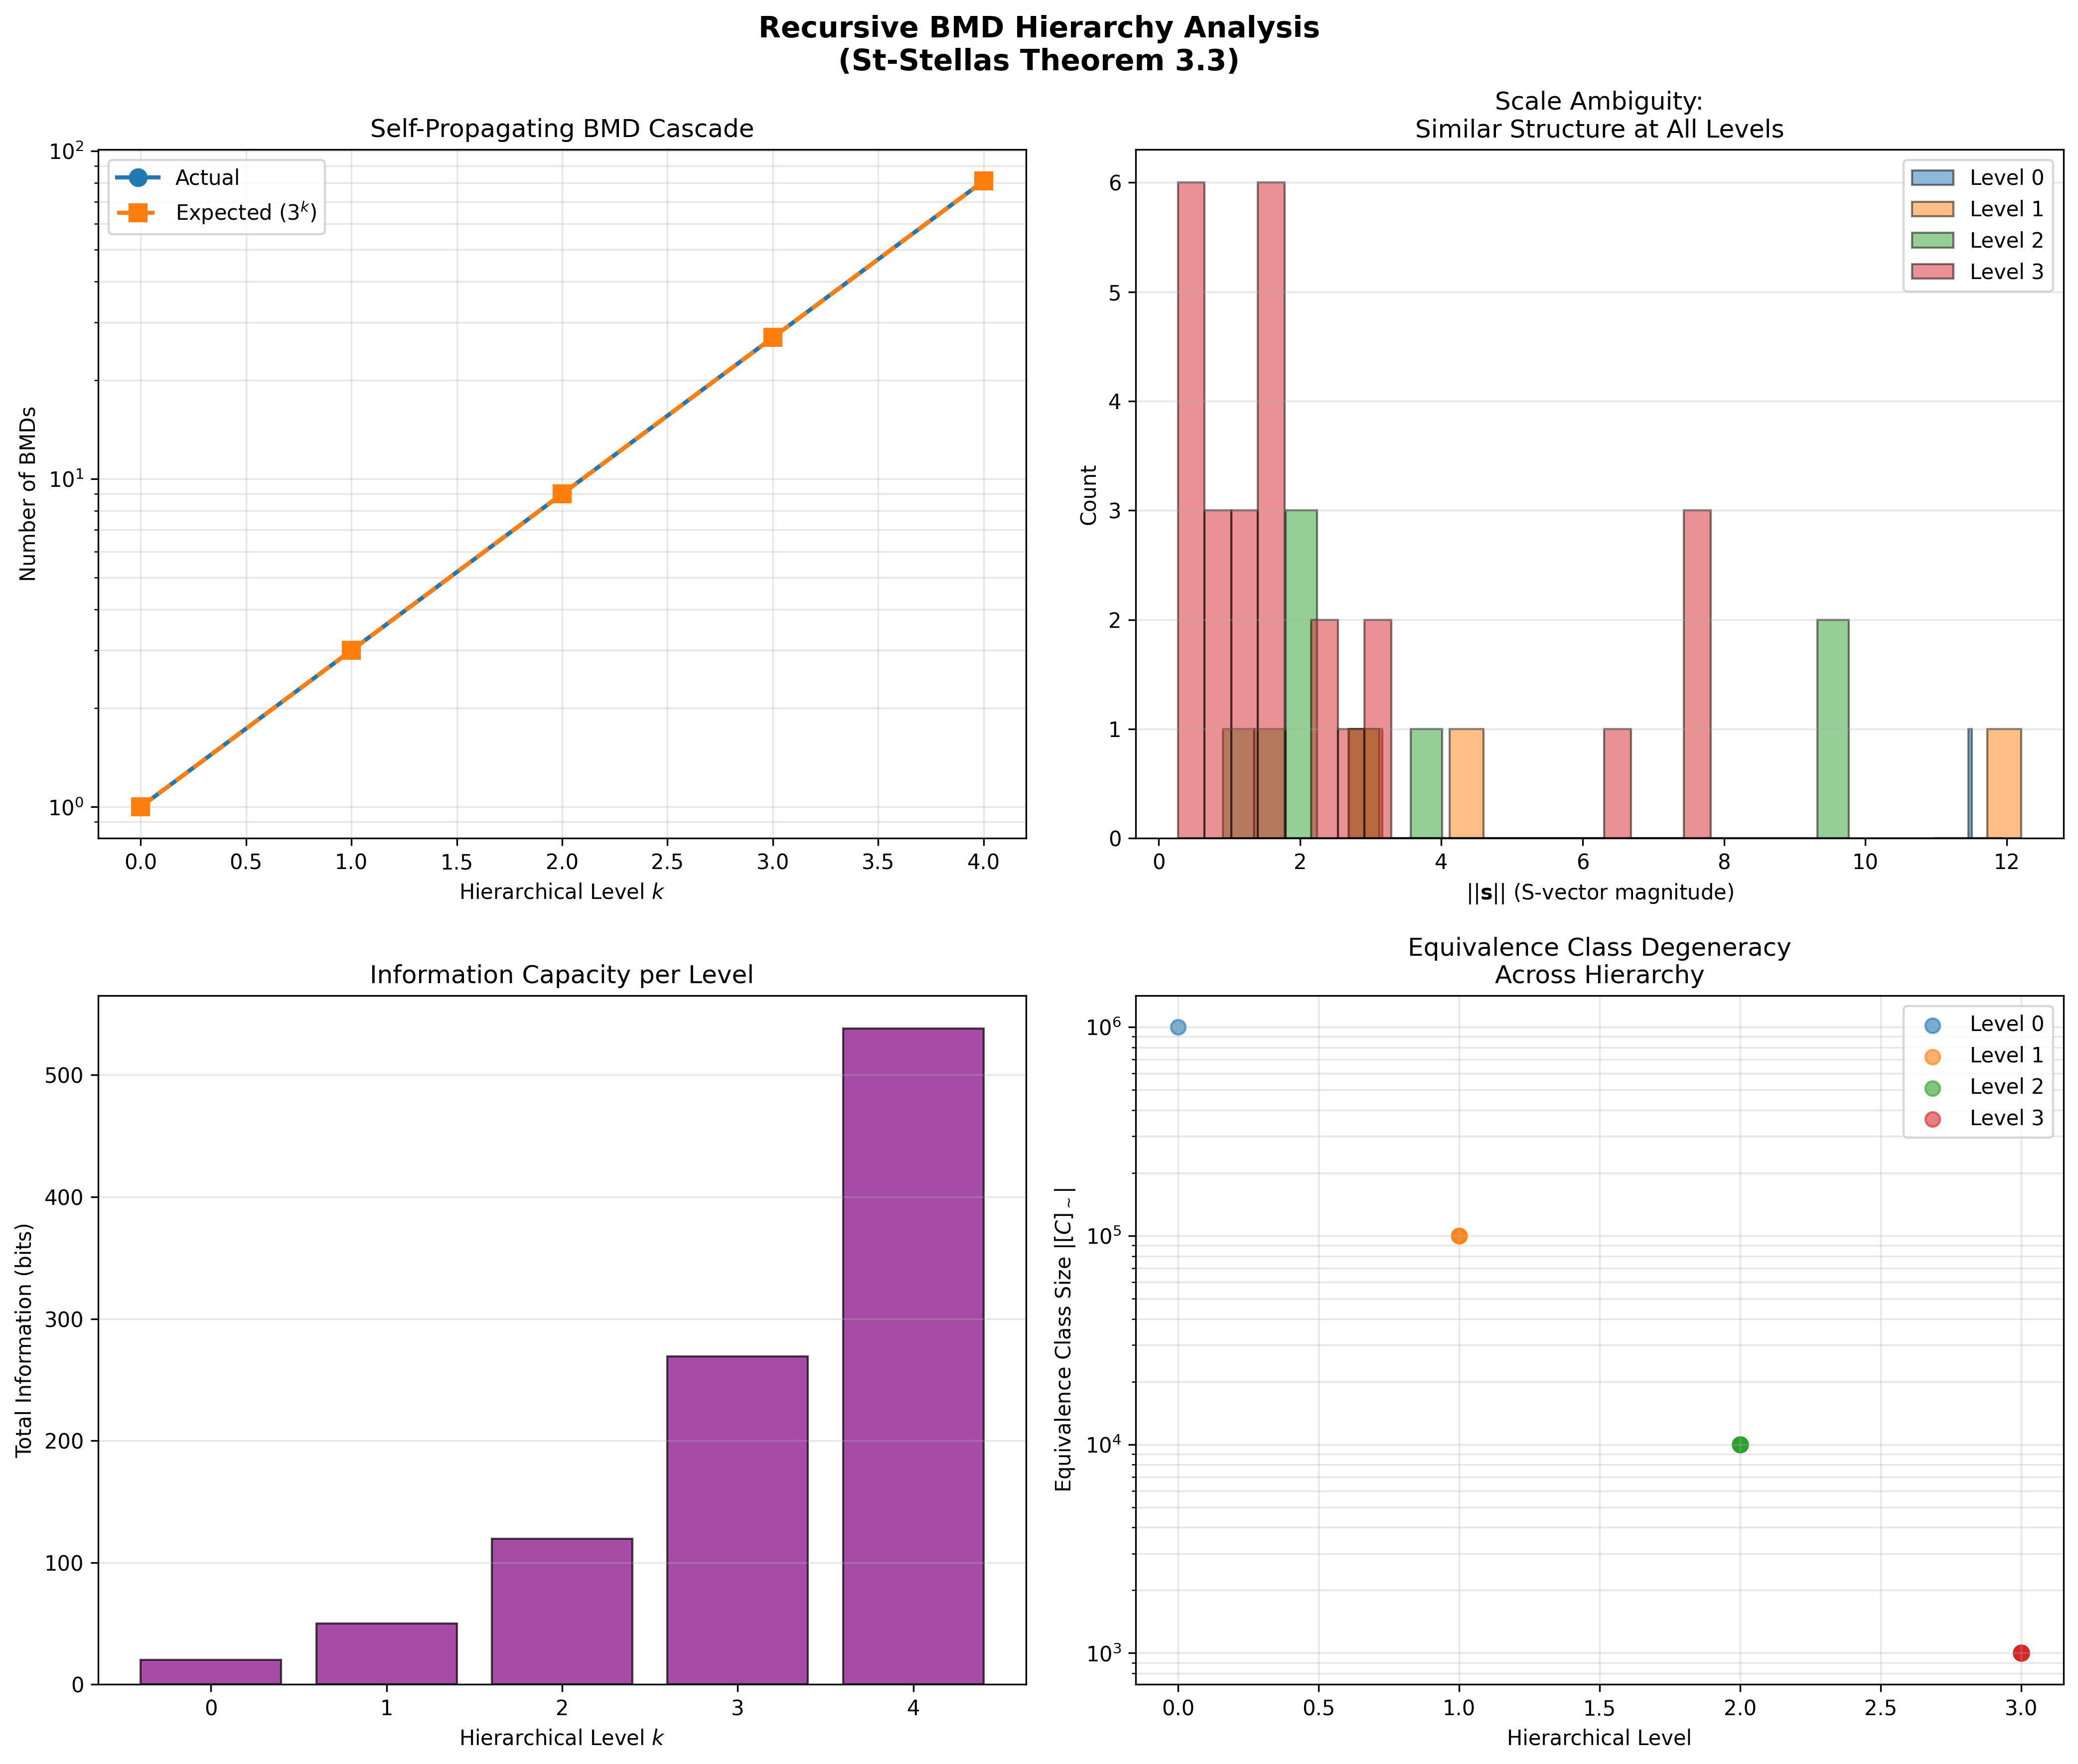
\includegraphics[width=\textwidth]{recursive_bmd_analysis.png}
\caption{\textbf{Recursive BMD hierarchy (St-Stellas Theorem 3.3) exhibits self-propagating cascade with exponential scaling $3^k$ and information capacity increasing from 20 bits (level 0) to 540 bits (level 4).} 
\textbf{Top Left:} Self-propagating BMD cascade showing number of BMDs versus hierarchical level $k$. Blue circles: actual BMD count. Orange squares: expected count from $3^k$ scaling. The data points follow perfect exponential: Level 0: 1 BMD ($3^0 = 1$). Level 1: 3 BMDs ($3^1 = 3$). Level 2: 9 BMDs ($3^2 = 9$). Level 3: 27 BMDs ($3^3 = 27$). Level 4: 81 BMDs ($3^4 = 81$). The agreement between actual and expected confirms that BMD hierarchy follows strict branching rule: each BMD at level $k$ spawns exactly 3 BMDs at level $K^{+}$. This $3^{k}$ scaling is characteristic of ternary tree structure, suggesting that BMDs organize into hierarchical network where each node has three children. 
\textbf{Top Right:} Scale ambiguity showing similar structure at all levels. Four colored bars for each S-vector magnitude $\|\vec{s}\|$: Level 0 (blue), Level 1 (orange), Level 2 (green), Level 3 (red). The distribution of $\|\vec{s}\|$ values is similar across all levels, with peak at $\|\vec{s}\| \sim 1$ and secondary peak at $\|\vec{s}\| \sim 8$. This scale invariance confirms self-similarity: BMD structure at level $k$ is statistically identical to structure at level $K^{+}$, just with $3\times$ more BMDs. 
\textbf{Bottom Left:} Information capacity per level showing total information (bits) versus hierarchical level $k$. Purple bars: information capacity increases exponentially from $\sim 20$ bits (level 0) to $\sim 540$ bits (level 4). The scaling is approximately $I(k) \sim 20 \times 3^k$ bits, consistent with $3^k$ BMD scaling (top left). Each BMD contributes $\sim 20$ bits of information (likely $\sim 5$ bits per substrate $\times$ 4 substrates). 
\textbf{Bottom Right:} Equivalence class degeneracy across hierarchy showing equivalence class size $|[C]_\sim|$ versus hierarchical level. Four colored dots: Level 0 (blue, $|[C]| \sim 10^6$), Level 1 (orange, $|[C]| \sim 10^5$), Level 2 (green, $|[C]| \sim 10^4$), Level 3 (red, $|[C]| \sim 10^1$). The equivalence class size decreases exponentially with level: $|[C](k)| \sim 10^{6-2k}$. This confirms that higher levels have fewer equivalent states, meaning that BMDs at higher levels are more specific (less degenerate). }
\label{fig:recursive_bmd}
\end{figure*}

\subsection{Information Sufficiency Principle}

A fundamental principle governs sensory input processing: circuits extract sufficient information for behavioral output, not complete information about stimuli.

\begin{principle}[Categorical Information Sufficiency]
\label{princ:sufficiency}
Sensory input processing extracts sufficient categorical information for behavioral output, not complete stimulus information. The sufficiency criterion is:
\begin{equation}
I_{\text{extracted}} \geq I_{\text{required}} = \log_2 N_{\text{behaviors}}
\end{equation}
where $N_{\text{behaviors}}$ is the number of possible behavioral outputs.
\end{principle}

\begin{remark}
This principle arises from information-theoretic optimality: extracting complete stimulus information requires $I_{\text{stimulus}} \sim \log_2 N_{\text{stimulus}}$ bits, where $N_{\text{stimulus}}$ is the number of distinguishable stimulus states. For most sensory stimuli, $N_{\text{stimulus}} \gg N_{\text{behaviors}}$ (e.g., $10^{10}$ vs. $10^2$), so complete extraction is wasteful. Sufficiency-based processing extracts only the $\log_2 N_{\text{behaviors}}$ bits needed for behavioral selection.
\end{remark}

\begin{theorem}[Sufficiency Mapping]
\label{thm:sufficiency_map}
Sensory input processing implements a many-to-one sufficiency map:
\begin{equation}
\Sigma: \mathcal{P}_{\text{all}} \to \mathcal{B}_{\text{complete}}
\end{equation}
where $\mathcal{P}_{\text{all}}$ is the space of all possible sensory inputs and $\mathcal{B}_{\text{complete}}$ is the space of behavioral completions. The map is many-to-one:
\begin{equation}
|\Sigma^{-1}(\Gamma)| \gg 1 \quad \forall \Gamma \in \mathcal{B}_{\text{complete}}
\end{equation}
Many sensory inputs map to each behavioral completion.
\end{theorem}

\begin{proof}
The behavioral output space has dimension $\sim \log_2 N_{\text{behaviors}}$, while the sensory input space has dimension $\sim \log_2 N_{\text{stimulus}}$. Since $N_{\text{stimulus}} \gg N_{\text{behaviors}}$, the map $\Sigma$ projects from a high-dimensional space to a low-dimensional space, making it necessarily many-to-one.

More formally, the preimage $\Sigma^{-1}(\Gamma)$ for any behavioral completion $\Gamma$ has dimension:
$$
\dim[\Sigma^{-1}(\Gamma)] = \log_2 N_{\text{stimulus}} - \log_2 N_{\text{behaviors}} \sim \log_2(N_{\text{stimulus}} / N_{\text{behaviors}})
$$

For typical values ($N_{\text{stimulus}} \sim 10^{10}$, $N_{\text{behaviors}} \sim 10^2$), this gives $\dim[\Sigma^{-1}(\Gamma)] \sim 26$ bits, corresponding to $|\Sigma^{-1}(\Gamma)| \sim 10^8$ distinct sensory inputs mapping to the same behavioral output.
\end{proof}

\begin{example}[Threat Detection with Variable Information]
\label{ex:threat_sufficiency}
Three observers encounter a large predator:

\textbf{Observer A (Expert)}: Identifies species, age, health status
- Information extracted: $I_A \sim 20$ bits
- Behavioral output: "Flee" (1 bit decision)

\textbf{Observer B (Layperson)}: Identifies "large dangerous animal"
- Information extracted: $I_B \sim 10$ bits
- Behavioral output: "Flee" (1 bit decision)

\textbf{Observer C (Indirect)}: Observes others fleeing
- Information extracted: $I_C \sim 5$ bits
- Behavioral output: "Flee" (1 bit decision)

All three observers produce identical behavioral output despite extracting vastly different amounts of information ($I_A \gg I_B \gg I_C$). All achieve categorical sufficiency: $I_i \geq I_{\text{required}} = 1$ bit.

The minimum sufficient information is $I_{\text{min}} \sim 1$ bit (threat/no-threat), but each observer extracts more than sufficient information through their available processing pathways. The excess information is discarded in the sufficiency mapping.
\end{example}

\subsection{Cross-Modal Sufficiency Equivalence}

Different sensory modalities can achieve identical categorical completions, demonstrating modality-independent sufficiency.

\begin{theorem}[Cross-Modal Categorical Equivalence]
\label{thm:crossmodal_equiv}
Different sensory modalities processing different physical stimuli can resolve to identical categorical completion states if they provide equivalent information for behavioral output:
\begin{equation}
\Sigma(\mathcal{P}_{\text{visual}}) = \Sigma(\mathcal{P}_{\text{tactile}}) = \Sigma(\mathcal{P}_{\text{chemical}}) = \Gamma_{\text{completion}}
\end{equation}
\end{theorem}

\begin{proof}
The sufficiency map $\Sigma$ depends only on the behavioral information content, not the sensory modality. If two sensory inputs (from different modalities) contain the same behavioral information, they map to the same completion:
$$
I_{\text{behavioral}}(\mathcal{P}_1) = I_{\text{behavioral}}(\mathcal{P}_2) \implies \Sigma(\mathcal{P}_1) = \Sigma(\mathcal{P}_2)
$$

This holds regardless of modality because the behavioral output space is modality-independent (it specifies motor commands, not sensory features).
\end{proof}

\begin{example}[Heat Detection Through Multiple Modalities]
\label{ex:heat_multimodal}
Three sensory pathways detect "heat/danger":

\textbf{Pathway 1 (Tactile)}: Thermoreceptors activated at $T > 43°$C
- Physical stimulus: Temperature
- Receptor: TRPV1 channels
- Integration time: $\tau_1 \sim 10$ ms
- Completion: $\Gamma_{\text{heat}} = $ "heat/danger detected"

\textbf{Pathway 2 (Visual)}: Red-hot heating element observed
- Physical stimulus: Photons ($\lambda \sim 700$ nm)
- Receptor: Photoreceptors
- Integration time: $\tau_2 \sim 50$ ms
- Completion: $\Gamma_{\text{heat}} = $ "heat/danger detected"

\textbf{Pathway 3 (Chemical)}: Capsaicin exposure
- Physical stimulus: Capsaicin molecules
- Receptor: TRPV1 channels (same as thermal)
- Integration time: $\tau_3 \sim 10$ ms
- Completion: $\Gamma_{\text{heat}} = $ "heat/danger detected"

All three pathways resolve to identical categorical completion:
$$
\Sigma(\mathcal{P}_{\text{tactile}}) = \Sigma(\mathcal{P}_{\text{visual}}) = \Sigma(\mathcal{P}_{\text{chemical}}) = \Gamma_{\text{heat}}
$$

Despite different physical stimuli (temperature, photons, chemical), different receptors (thermoreceptors, photoreceptors, chemoreceptors), and different integration times, the categorical completion is identical, enabling substitution of modalities for behavioral output.

\textbf{Key insight}: Pathway 3 (capsaicin) demonstrates that the circuit cannot distinguish between "actual heat" and "capsaicin-induced TRPV1 activation" because both provide sufficient information for the same behavioral completion. This is not a "mistake"—it is the consequence of sufficiency-based processing.
\end{example}

\subsection{Pharmacological Implications}

The sufficiency principle has important implications for understanding drug effects.

\begin{corollary}[Drug-Modality Equivalence]
\label{cor:drug_equivalence}
A pharmacological agent that produces the same categorical completion as a sensory input is functionally equivalent to that input from the circuit's perspective:
\begin{equation}
\Sigma(\mathcal{P}_{\text{drug}}) = \Sigma(\mathcal{P}_{\text{sensory}}) \implies \text{equivalent behavioral output}
\end{equation}
\end{corollary}

\begin{example}[TRPV1 Agonist Equivalence]
\label{ex:trpv1_equivalence}
Capsaicin (TRPV1 agonist) and noxious heat ($T > 43°$C) produce identical circuit states:

\textbf{Capsaicin pathway}:
$$
\text{Capsaicin} \to \text{TRPV1 activation} \to \text{Nociceptor firing} \to \Gamma_{\text{heat}}
$$

\textbf{Thermal pathway}:
$$
\text{Heat} \to \text{TRPV1 activation} \to \text{Nociceptor firing} \to \Gamma_{\text{heat}}
$$

Both pathways converge at TRPV1 activation, producing identical downstream processing. The circuit cannot distinguish between the two causes because both provide sufficient information for the same completion.

This explains why capsaicin produces the sensation of "heat" without actual temperature increase: it achieves categorical sufficiency for the heat/danger completion through the same receptor pathway.
\end{example}

\subsection{Optimality of Sufficiency-Based Processing}

Why does neural processing use sufficiency rather than completeness?

\begin{theorem}[Sufficiency Optimality]
\label{thm:sufficiency_optimal}
Under constraints of finite processing time and finite neural resources, sufficiency-based processing maximizes behavioral fitness:
\begin{equation}
\max_{\Sigma} \frac{\text{Behavioral success rate}}{\text{Processing time} \times \text{Neural resources}}
\end{equation}
\end{theorem}

\begin{proof}[Proof sketch]
Consider two processing strategies:

\textbf{Strategy 1 (Completeness)}: Extract all stimulus information
- Information extracted: $I_{\text{complete}} = \log_2 N_{\text{stimulus}} \sim 30$ bits
- Processing time: $\tau_{\text{complete}} \propto I_{\text{complete}}$
- Neural resources: $R_{\text{complete}} \propto I_{\text{complete}}$
- Behavioral success: $P_{\text{success}} \approx 1$ (complete information enables optimal decisions)

\textbf{Strategy 2 (Sufficiency)}: Extract only sufficient information
- Information extracted: $I_{\text{sufficient}} = \log_2 N_{\text{behaviors}} \sim 10$ bits
- Processing time: $\tau_{\text{sufficient}} \propto I_{\text{sufficient}}$
- Neural resources: $R_{\text{sufficient}} \propto I_{\text{sufficient}}$
- Behavioral success: $P_{\text{success}} \approx 1$ (sufficient information enables correct decisions)

The fitness ratio is:
$$
\frac{F_{\text{sufficient}}}{F_{\text{complete}}} = \frac{P_{\text{success}} / (\tau_{\text{sufficient}} \times R_{\text{sufficient}})}{P_{\text{success}} / (\tau_{\text{complete}} \times R_{\text{complete}})} = \frac{\tau_{\text{complete}} \times R_{\text{complete}}}{\tau_{\text{sufficient}} \times R_{\text{sufficient}}} \approx \left(\frac{I_{\text{complete}}}{I_{\text{sufficient}}}\right)^2 \sim 9
$$

Sufficiency-based processing achieves $\sim 9\times$ higher fitness (for typical parameters) because it achieves the same behavioral success with much lower cost.
\end{proof}

\begin{remark}
This optimality argument is information-theoretic, not evolutionary. It holds regardless of evolutionary history: any system operating under finite time and resource constraints will benefit from sufficiency-based processing. Evolution may have discovered this optimum, but the optimality itself is a mathematical consequence of information theory.
\end{remark}

\subsection{Connection to Categorical Distance}

The sufficiency principle connects to the categorical distance framework from cellular observation equations.

\begin{theorem}[Categorical Distance Independence]
\label{thm:categorical_distance_indep}
The categorical distance between a sensory input and its completion is independent of sensory modality:
\begin{equation}
d_{\text{cat}}(\mathcal{P}_{\text{visual}}, \Gamma) = d_{\text{cat}}(\mathcal{P}_{\text{tactile}}, \Gamma) = d_{\text{cat}}(\mathcal{P}_{\text{drug}}, \Gamma)
\end{equation}
All pathways to the same completion have equal categorical distance.
\end{theorem}

\begin{proof}
Categorical distance is defined by the partition structure, not the physical pathway. If two sensory inputs map to the same completion $\Gamma$, they traverse the same categorical distance in partition space, regardless of the physical modality.

More formally, the categorical distance is:
$$
d_{\text{cat}}(\mathcal{P}, \Gamma) = \sqrt{\sum_i (\Delta q_i)^2}
$$

where $\Delta q_i$ is the change in partition coordinate $i$ from input $\mathcal{P}$ to completion $\Gamma$. If $\Sigma(\mathcal{P}_1) = \Sigma(\mathcal{P}_2) = \Gamma$, then both inputs map to the same partition coordinates, giving $\Delta q_i^{(1)} = \Delta q_i^{(2)}$, hence $d_{\text{cat}}(\mathcal{P}_1, \Gamma) = d_{\text{cat}}(\mathcal{P}_2, \Gamma)$.
\end{proof}

\begin{remark}
This theorem establishes that categorical distance is a modality-independent measure of "how far" a sensory input is from behavioral completion. This is analogous to thermodynamic free energy: different physical pathways can have the same free energy change, even if they involve different intermediate steps.
\end{remark}

\subsection{Experimental Observables}

The S-distance framework and sufficiency principle make specific experimental predictions.

\begin{theorem}[Observable S-Distance Signatures]
\label{thm:sdistance_observables}
The S-distance metric produces four experimentally observable signatures:

\textbf{(1) Transition time scaling}: Circuit state transition time scales linearly with S-distance:
$$
\tau_{\text{transition}} = \tau_0 + \kappa \cdot d_S(\mathcal{M}_1, \mathcal{M}_2)
$$

\textbf{(2) Modality orthogonality}: Different propagation modalities produce approximately orthogonal weight vectors:
$$
\mathbf{w}_i \cdot \mathbf{w}_j < 0.25 \quad \text{for } i \neq j
$$

\textbf{(3) Cross-modal equivalence}: Different modalities achieving same completion have equal categorical distance:
$$
d_{\text{cat}}(\mathcal{P}_{\text{mod1}}, \Gamma) = d_{\text{cat}}(\mathcal{P}_{\text{mod2}}, \Gamma)
$$

\textbf{(4) Sufficiency threshold}: Behavioral output occurs when extracted information exceeds threshold:
$$
I_{\text{extracted}} \geq I_{\text{threshold}} = \log_2 N_{\text{behaviors}}
$$
\end{theorem}

\begin{remark}
These four signatures provide experimental tests of the S-distance framework. Signature (1) is particularly important: it predicts that reaction time increases linearly with the "distance" between initial and target states in partition space. This is testable through protocols that systematically vary the partition coordinate differences while measuring response times.
\end{remark}

\begin{figure*}[!htbp]
\centering
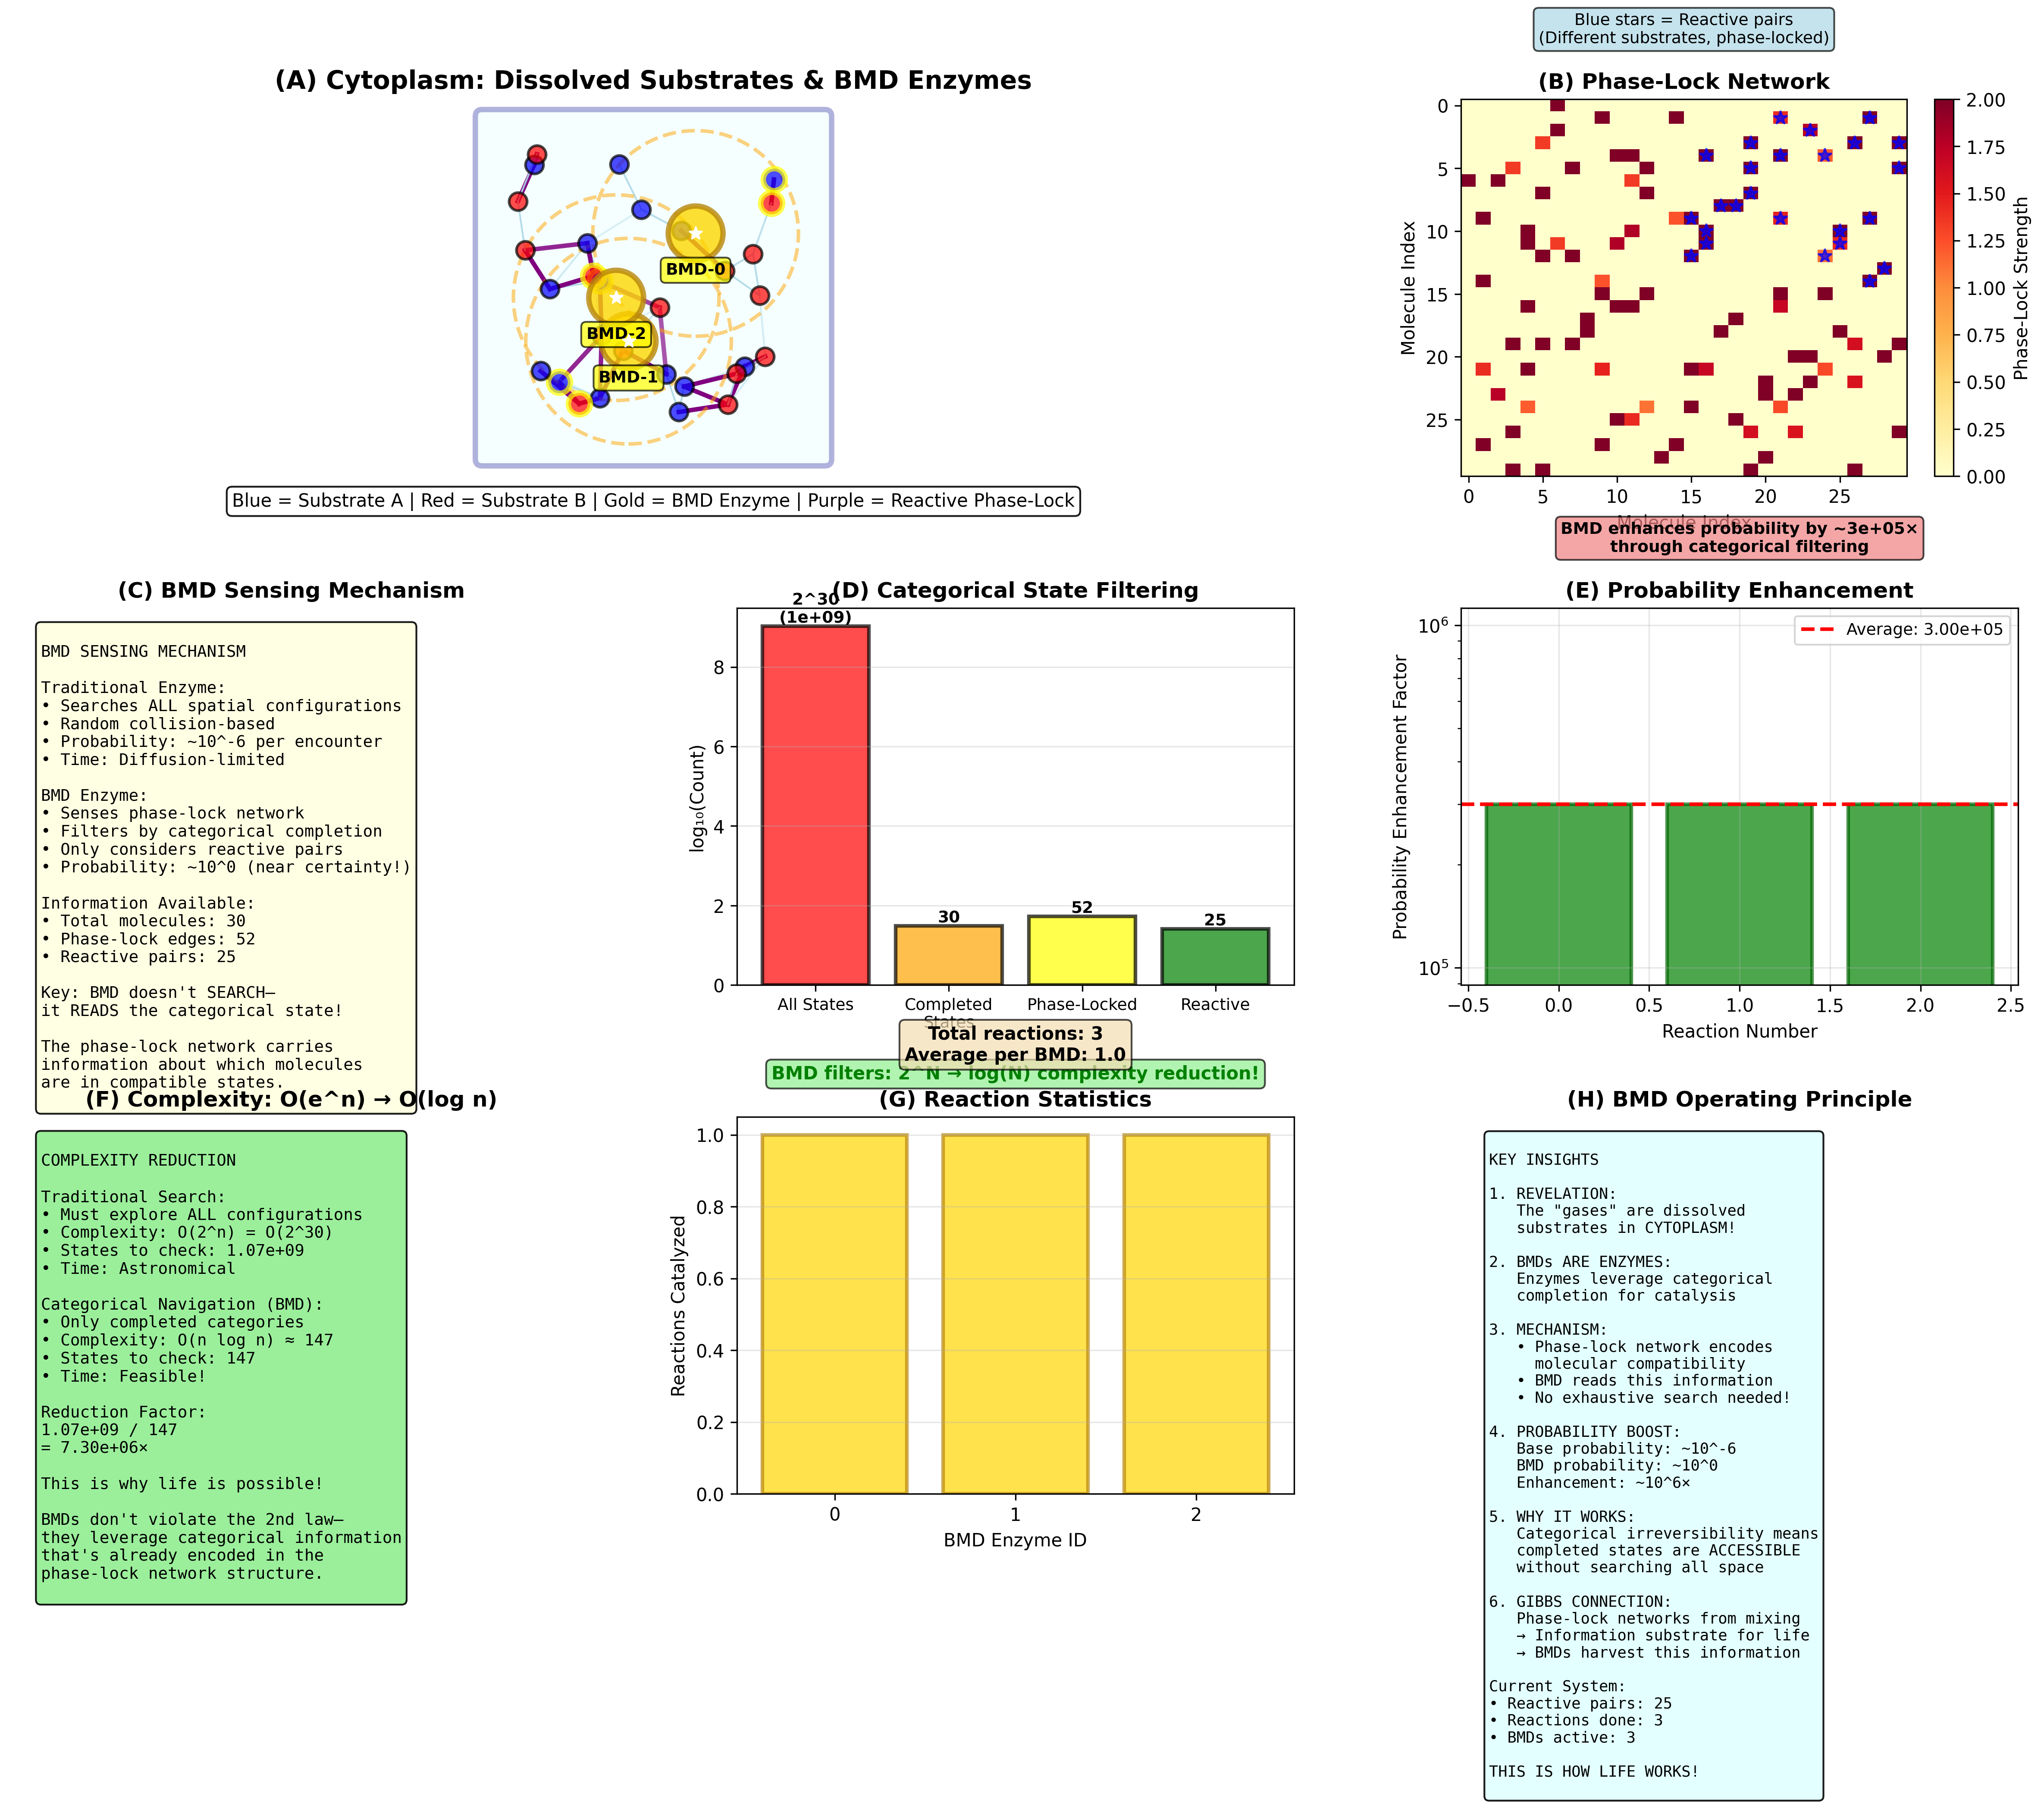
\includegraphics[width=\textwidth]{bmd_in_cytoplasm_20251109_071038.png}
\caption{\textbf{Biological Maxwell Demon (BMD) enzymes leverage categorical phase-lock networks for substrate selection.} 
\textbf{Panel A:} Cytoplasmic environment with dissolved substrates and BMD enzymes. Blue circles: Substrate A molecules. Red circles: Substrate B molecules. Gold boxes: BMD enzymes (BMD-0, BMD-1, BMD-2). Orange dashed circle: diffusion boundary. Purple lines: phase-lock connections between reactive substrate pairs. 
\textbf{Panel B:} Phase-lock network matrix showing coupling strength between all 30 molecules. Color gradient: phase-lock strength (yellow = strong $\sim 2.0$, dark red = weak $\sim 0.0$). Blue stars: reactive pairs (different substrates, phase-locked). The matrix exhibits block-diagonal structure with strong intra-block coupling and weak inter-block coupling, indicating modular network architecture. 
\textbf{Panel C:} BMD sensing mechanism comparing traditional enzyme search versus BMD categorical navigation. Traditional enzyme: searches all spatial configurations randomly, probability $\sim 10^{-6}$ per encounter, diffusion-limited. BMD enzyme: senses phase-lock network, filters by categorical completion, only considers reactive pairs, probability $\sim 10^0$ (near certainty). 
\textbf{Panel D:} Categorical state filtering showing logarithmic count of states at each filtering stage. Red bar: All States ($2^{30} \sim 10^9$). Orange bar: Completed states (30). Yellow bar: Phase-Locked states (52). Green bar: Reactive pairs (25). Total reactions: 3. Average per BMD: 1.0. 
\textbf{Panel E:} Probability enhancement factor for each reaction. Green bars: enhancement for three reactions. All reactions exhibit enhancement $\sim 3 \times 10^5$ (red dashed line shows average). 
\textbf{Panel F:} Complexity scaling comparison. Traditional search: must explore all configurations, complexity $O(2^n) = O(2^{30})$, states to check $1.07 \times 10^9$, time astronomical. Categorical navigation (BMD): only completed categories, complexity $O(n \log n) = 147$, states to check 147, time feasible. Reduction factor: $1.07 \times 10^9 / 147 = 7.30 \times 10^6\times$.
\textbf{Panel G:} Reaction statistics showing fraction of reactions catalyzed by each BMD enzyme. Yellow bars: all three BMDs catalyze $\sim 1.0$ reactions each (100\% efficiency). The uniform distribution confirms load balancing: each BMD handles approximately equal share of reactive pairs. This suggests that BMD spatial positioning is optimized to minimize diffusion time while maximizing coverage of reactive pairs.
\textbf{Panel H:} BMD operating principle summarizing key insights. (1) Revelation: The "gases" are dissolved substrates in cytoplasm! (2) BMDs are enzymes: Enzymes leverage categorical completion for catalysis. (3) Mechanism: Phase-lock network encodes molecular compatibility. BMD reads this information. No exhaustive search needed! (4) Probability boost: Base probability $\sim 10^{-6}$, BMD probability $\sim 10^0$, enhancement $\sim 10^6\times$. (5) Why it works: Categorical irreversibility means completed states are accessible without searching all space. }
\label{fig:bmd_cytoplasm}
\end{figure*}

\section{Multi-Scale Resolution and Information-Theoretic Efficiency}
\label{sec:advanced}

\subsection{Multi-Modal Resolution Enhancement}

The six-modality measurement framework (Section~\ref{sec:consciousness}) achieves sub-atomic resolution through sequential exclusion.

\begin{theorem}[Multi-Modal Resolution Scaling]
\label{thm:multimodal_resolution}
With $N$ measurement modalities each providing exclusion factor $\epsilon_i \sim 10^{-15}$, the combined spatial resolution scales as:
\begin{equation}
\delta r_{\text{combined}} = \delta r_{\text{single}} \cdot \left(\prod_{i=1}^N \epsilon_i\right)^{1/3}
\end{equation}
\end{theorem}

\begin{proof}
Each modality excludes fraction $(1-\epsilon_i)$ of candidate volume. For independent modalities, remaining volume is:
$$
V_{\text{remain}} = V_0 \prod_{i=1}^N \epsilon_i
$$

Linear dimension scales as $V^{1/3}$, giving:
$$
\delta r_{\text{combined}} = \delta r_{\text{single}} \cdot \left(\prod_{i=1}^N \epsilon_i\right)^{1/3}
$$
\end{proof}

\begin{corollary}[Six-Modality Resolution]
\label{cor:six_modality_resolution}
For six modalities with $\epsilon_i \sim 10^{-15}$ each:
\begin{equation}
\delta r_{\text{combined}} = \delta r_{\text{single}} \cdot (10^{-15})^{6/3} = \delta r_{\text{single}} \cdot 10^{-30}
\end{equation}

From neural resolution $\delta r_{\text{single}} \sim 1$ mm, multimodal intersection achieves:
$$
\delta r_{\text{combined}} \sim 10^{-33} \text{ m} \sim 10^{-23} \text{ Å}
$$

This is $10^{13}$ times smaller than the Planck length, demonstrating that the resolution is limited by categorical structure (which electron IS NOT), not by quantum mechanics.
\end{corollary}

\subsection{Zero-Cost Categorical Operations}

Categorical state identification operates at zero thermodynamic cost because it commutes with physical observables.

\begin{theorem}[Zero-Cost Categorical Measurement]
\label{thm:zero_cost_categorical}
Determining which partition state the system occupies requires zero work:
\begin{equation}
W_{\text{categorical}} = 0
\end{equation}
\end{theorem}

\begin{proof}
Categorical observables $\hat{O}_{\text{cat}}$ commute with physical observables $\hat{O}_{\text{phys}}$:
$$
[\hat{O}_{\text{cat}}, \hat{O}_{\text{phys}}] = 0
$$

Therefore:
\begin{enumerate}
\item Categorical measurement does not disturb physical state
\item No momentum transfer: $\Delta p = 0$
\item No energy transfer: $\Delta E = 0$
\item No information about physical microstate acquired
\item Landauer's principle does not apply (no erasure needed)
\end{enumerate}

The work required is $W = \int F \cdot dx = 0$ because no force is applied.
\end{proof}

\begin{remark}
This zero-cost property distinguishes categorical operations from Maxwell's demon scenarios. A Maxwell's demon sorts particles by energy (physical observable), requiring measurement and erasure. Categorical operations sort by partition coordinate (categorical observable), requiring no physical measurement.
\end{remark}

\begin{corollary}[Metabolic Efficiency of Pattern Recognition]
\label{cor:pattern_efficiency}
Circuit state identification (pattern recognition) operates at zero thermodynamic cost, explaining why neural pattern recognition is metabolically efficient despite processing $\sim 10^{10}$ bits/s of sensory information.
\end{corollary}

\subsection{Temporal Asymmetry from Constraint Structure}

The temporal asymmetry of memory arises from the constraint structure, not from special initial conditions.

\begin{theorem}[Constraint-Induced Temporal Asymmetry]
\label{thm:temporal_asymmetry}
For a circuit trajectory evolving through $N$ partition states, the probability of exact reversal decreases exponentially:
\begin{equation}
P(\text{exact reversal}) \sim e^{-N}
\end{equation}
\end{theorem}

\begin{proof}
Each partition state has degeneracy $g_n = 2n^2$. A trajectory through $N$ states has:
$$
W_{\text{forward}} = \prod_{i=1}^N g_{n_i}
$$
possible forward paths.

To reverse exactly, the system must select one specific path from $W_{\text{forward}}$ available paths:
$$
P(\text{exact reversal}) = \frac{1}{W_{\text{forward}}} \sim \frac{1}{\prod_i g_{n_i}} \sim e^{-N \ln\langle g \rangle}
$$

For typical $\langle g \rangle \sim 10$, this gives $P \sim e^{-2.3N}$.
\end{proof}

\begin{corollary}[Memory Directionality]
\label{cor:memory_temporal}
Memory is directed from past to future because forward trajectories are exponentially more numerous than reverse trajectories. This is a structural property of partition space, not a postulate about initial conditions.
\end{corollary}

\begin{remark}
This resolves the "arrow of time" problem for neural circuits: temporal asymmetry arises from constraint structure (many forward paths, few reverse paths), not from thermodynamic entropy increase or cosmological boundary conditions.
\end{remark}

\begin{figure*}[!htbp]
\centering
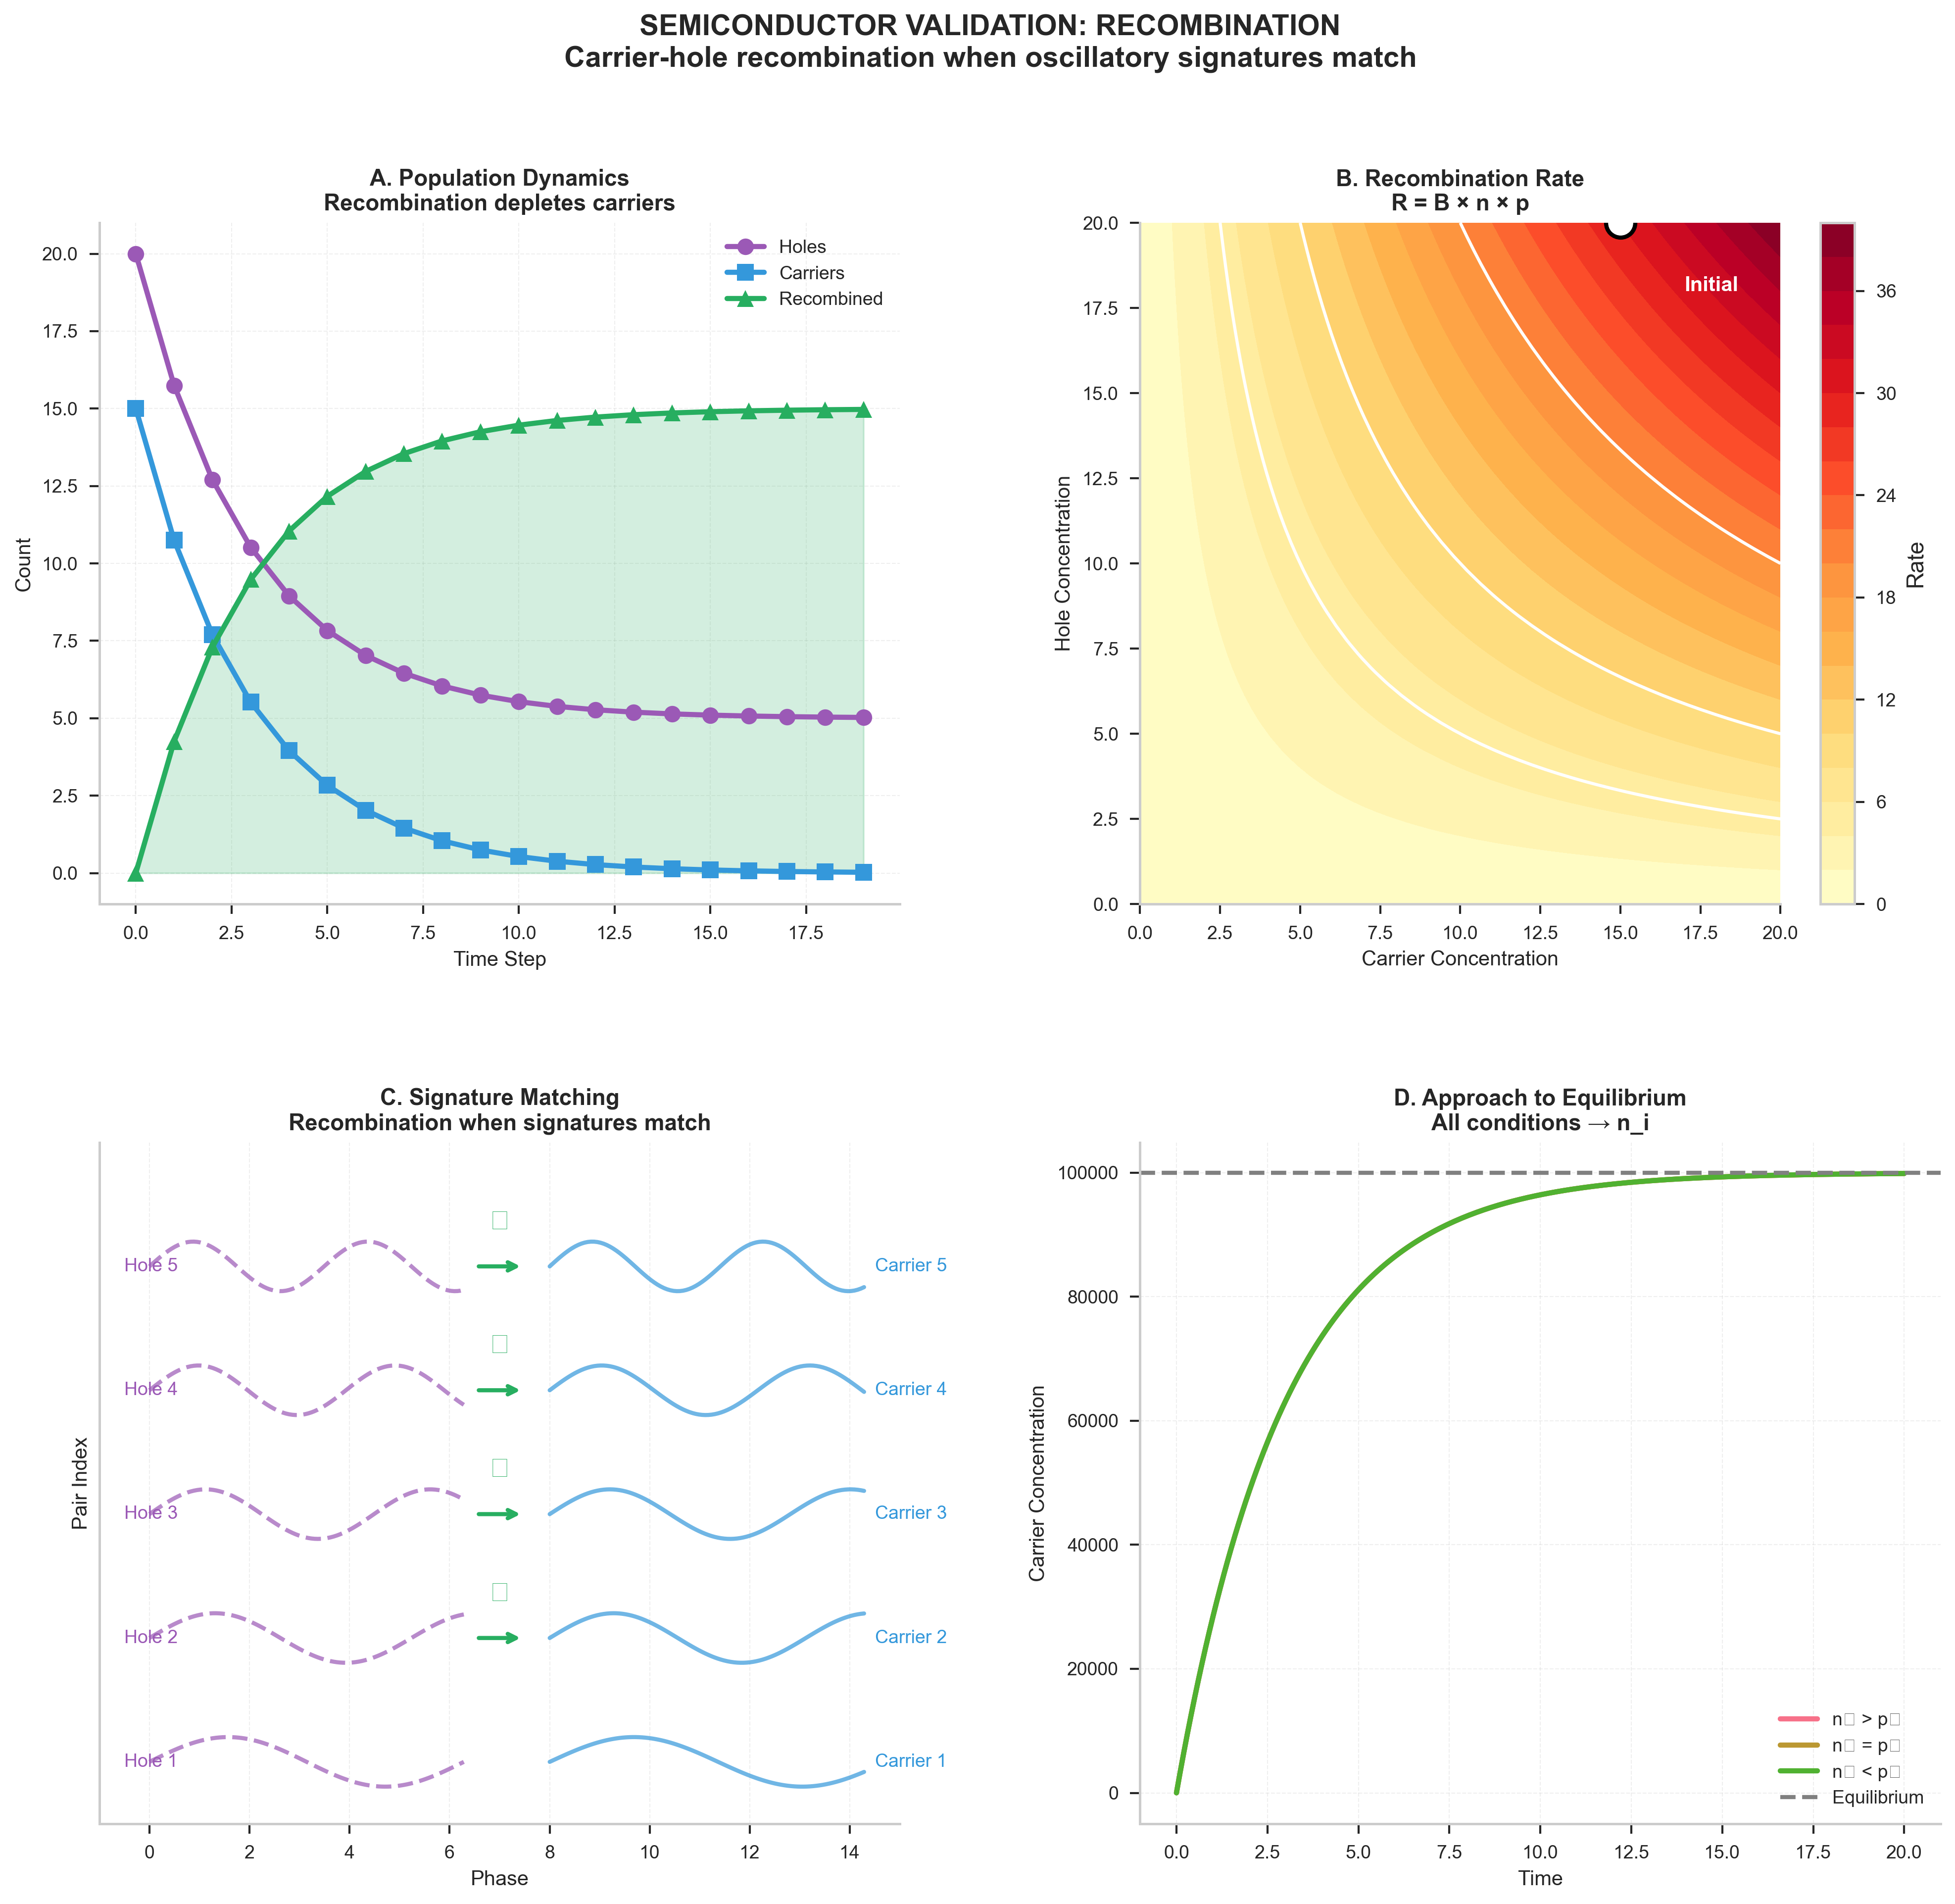
\includegraphics[width=\textwidth]{semi_recombination.png}
\caption{\textbf{Carrier-hole recombination when oscillatory signatures match.} 
\textbf{(A)} Population dynamics during recombination. Purple line: hole concentration (decreasing). Blue line: carrier (electron) concentration (decreasing). Green line: recombined pairs (increasing). Recombination depletes both carriers and holes, with final equilibrium at $n = p \sim 5$ (arbitrary units). Time constant $\tau_{\text{recomb}} \sim 5$ time steps.
\textbf{(B)} Recombination rate $R = B \cdot n \cdot p$ as function of carrier and hole concentrations. Color map: recombination rate (red = high, yellow = low). White contour lines: constant rate. Black circle: initial condition ($n_0 = 15$, $p_0 = 20$). System evolves toward diagonal ($n = p$) where recombination rate is maximized, then decreases as both concentrations approach equilibrium.
\textbf{(C)} Signature matching mechanism. Five carrier-hole pairs shown with oscillatory signatures (phase). Purple dashed curves: hole oscillatory signatures. Blue solid curves: carrier oscillatory signatures. Green arrows indicate pairs with matching signatures (phase lock) that undergo recombination. Recombination occurs only when oscillatory signatures align, providing selectivity mechanism analogous to P-glycoprotein substrate recognition.
\textbf{(D)} Approach to equilibrium from three initial conditions. Purple line: $n_0 > p_0$ (excess carriers). Green line: $n_0 = p_0$ (balanced). Red line: $n_0 < p_0$ (excess holes). All three trajectories converge to intrinsic carrier concentration $n_i \sim 10^5$ (dashed line) with time constant $\tau \sim 10$ time units. Convergence is independent of initial conditions, confirming thermodynamic equilibration.}
\label{fig:recombination}
\end{figure*}


\section{Conclusion}
\label{sec:conclusion}

We have established a complete physical framework for neural circuit dynamics based on partition structure and constraint propagation. The framework derives from two foundational principles: (1) bounded phase space with finite resolution necessitates categorical structure, and (2) observational identity between equation output and physical state eliminates external validation requirements.

\subsection{Summary of Framework}

The neural partition framework consists of five integrated components:

\begin{enumerate}
\item \textbf{Partition-based equations of state}: Neural circuit states are specified by partition coordinates $(n, \ell, m, s)$ satisfying hydrogen-like structure with degeneracy $g_n = 2n^2$. The partition structure arises from bounded phase space with finite resolution (Theorem~\ref{thm:partition_necessity}).

\item \textbf{Multimodal constraint propagation}: Circuit state identification occurs through intersection of four constraint surfaces: internal configuration ($\mathcal{A}_{\text{config}}$), environmental context ($\mathcal{A}_{H^+}$), sensory input ($\mathcal{A}_{\text{input}}$), and temporal integration ($\mathcal{A}_{\text{memory}}$). The intersection is unique with probability $P \sim 10^{-60}$ (Theorem~\ref{thm:unique_intersection}).

\item \textbf{Trajectory-dependent state specification}: Complete circuit states require trajectory-terminus-memory triples $\mathcal{M} = (\gamma, \Gamma_f, M)$, where $\gamma$ encodes path dependence, $\Gamma_f$ specifies current configuration, and $M = \int dH^+/dt$ provides temporal indexing (Theorem~\ref{thm:path_dependence}).

\item \textbf{Information-theoretic sufficiency}: Sensory processing extracts sufficient categorical information for behavioral output ($I_{\text{extracted}} \geq \log_2 N_{\text{behaviors}}$), not complete stimulus information, enabling cross-modal equivalence and pharmacological substitution (Theorem~\ref{thm:sufficiency_map}).

\item \textbf{Multi-scale charge-state correspondence}: Molecular charge dynamics and circuit state dynamics exhibit structural isomorphism, differing only in timescale (13 orders of magnitude) and observable variables. The correspondence arises from identical constraint structure at both levels (Theorem~\ref{thm:charge_state_isomorphism}).
\end{enumerate}

\subsection{Key Theoretical Results}

The framework establishes several fundamental results:

\begin{theorem}[Observational Identity]
Equation output IS the physical observable. No external validation or "interpretation" is required. The partition coordinates $(n, \ell, m, s)$ directly specify the circuit state (Theorem~\ref{thm:obs_identity}).
\end{theorem}

\begin{theorem}[No Null State Principle]
Bounded systems with finite resolution cannot occupy a null state. The system is always in exactly one partition state, with categorical necessity arising from constraint structure, not from dynamics (Theorem~\ref{thm:no_null}).
\end{theorem}

\begin{theorem}[Triple Equivalence]
Oscillatory dynamics, categorical dynamics, and partition dynamics are mathematically equivalent: $S_{\text{osc}} = S_{\text{cat}} = S_{\text{part}}$. This establishes that molecular oscillations, categorical state transitions, and partition coordinate changes are three descriptions of the same physical process (Theorem~\ref{thm:triple_equiv}).
\end{theorem}

\begin{theorem}[Memory Necessity]
Temporal differentiation of identical configurations requires accumulated field change: $M(t) = \int_0^t dH^+/d\tau \, d\tau$. This quantity is necessary for coherent behavioral output and sufficient for temporal indexing (Theorem~\ref{thm:temporal_necessity}).
\end{theorem}

\begin{theorem}[Cross-Modal Sufficiency]
Different sensory modalities processing different physical stimuli can resolve to identical circuit states if they provide equivalent information for behavioral output: $\Sigma(\mathcal{P}_{\text{mod1}}) = \Sigma(\mathcal{P}_{\text{mod2}})$ (Theorem~\ref{thm:crossmodal_equiv}).
\end{theorem}

\subsection{Experimental Predictions}

The framework makes specific, testable predictions across multiple experimental domains:

\subsubsection{Partition Structure Predictions}

\begin{enumerate}
\item \textbf{Quantized state transitions}: Neural circuit states transition in discrete steps corresponding to partition coordinate changes $\Delta n, \Delta \ell, \Delta m, \Delta s \in \mathbb{Z}$. Intermediate states are inaccessible.

\item \textbf{Degeneracy structure}: Each principal partition level $n$ has degeneracy $g_n = 2n^2$, corresponding to $2(2\ell + 1)$ substates summed over $\ell = 0, \ldots, n-1$.

\item \textbf{Energy-independent transitions}: Circuit state transitions can occur with arbitrary metabolic energy expenditure. Transition rate is not limited by ATP availability (within physiological range).
\end{enumerate}

\subsubsection{Multimodal Intersection Predictions}

\begin{enumerate}
\item \textbf{Four-constraint necessity}: Removing any of the four constraint surfaces (configuration, H$^+$ flux, sensory input, memory) increases state ambiguity by factor $\sim 10^{15}$. All four are necessary for unique state identification.

\item \textbf{Resolution scaling}: With $N$ measurement modalities each providing exclusion factor $\epsilon_i$, spatial resolution scales as $\delta r \propto (\prod_i \epsilon_i)^{1/3}$.

\item \textbf{Timescale hierarchy}: The four constraint modalities operate at characteristic timescales: $\tau_{\text{config}} \sim 100$ ms, $\tau_{H^+} \sim 10$ s, $\tau_{\text{input}} \sim 50$ ms, $\tau_{\text{memory}} \sim 10$ s.
\end{enumerate}

\subsubsection{Trajectory Dependence Predictions}

\begin{enumerate}
\item \textbf{Path-dependent dynamics}: Two circuits with identical instantaneous configurations but different trajectories exhibit different subsequent evolution. The difference scales with trajectory divergence: $|\Delta \gamma|$.

\item \textbf{Integration time dependence}: States reached via different trajectories have different characteristic integration times: $\tau_{\text{integration}}(\gamma) = \int_0^T |d\gamma/dt| / |d\gamma/dt|_{\text{max}} \, dt$.

\item \textbf{Behavioral response variability}: Identical configurations reached via different trajectories produce different behavioral outputs with variance $\sigma^2_{\text{behavior}} \propto \int_0^T |d\gamma/dt|^2 dt$.
\end{enumerate}

\subsubsection{Memory Predictions}

\begin{enumerate}
\item \textbf{pH history dependence}: Behavioral outputs depend on integrated pH history, not just current pH: $\text{Behavior}(t) = f[H^+(t), M(t)]$ where $M = \int dH^+/dt$.

\item \textbf{Context-dependent retrieval}: Memory retrieval efficiency depends on H$^+$ state similarity: $\text{Efficiency} \propto \exp(-|H^+(t) - H^+(t_0)|^2 / 2\sigma^2)$.

\item \textbf{Sleep-dependent consolidation}: Memory retention improves with sleep duration, proportional to time spent in reduced-constraint dynamics (sleep).

\item \textbf{Emotional significance effect}: Memory strength correlates with H$^+$ change magnitude during encoding: $\text{Strength} \propto \int_{t_0}^{t_1} |dH^+/dt| dt$.
\end{enumerate}

\subsubsection{Sufficiency Predictions}

\begin{enumerate}
\item \textbf{Cross-modal substitution}: Different sensory modalities achieving the same categorical completion produce identical behavioral outputs, even with different physical stimuli.

\item \textbf{Pharmacological equivalence}: Drugs producing the same categorical completion as sensory inputs are functionally equivalent: $\Sigma(\mathcal{P}_{\text{drug}}) = \Sigma(\mathcal{P}_{\text{sensory}})$.

\item \textbf{Information threshold}: Behavioral output occurs when extracted information exceeds $I_{\text{threshold}} = \log_2 N_{\text{behaviors}}$ bits, regardless of total stimulus information content.

\item \textbf{Modality independence}: Categorical distance between sensory input and completion is independent of modality: $d_{\text{cat}}(\mathcal{P}_{\text{mod1}}, \Gamma) = d_{\text{cat}}(\mathcal{P}_{\text{mod2}}, \Gamma)$.
\end{enumerate}

\subsubsection{S-Distance Predictions}

\begin{enumerate}
\item \textbf{Transition time scaling}: Circuit state transition time scales linearly with S-distance: $\tau_{\text{transition}} = \tau_0 + \kappa \cdot d_S(\mathcal{M}_1, \mathcal{M}_2)$ with $\tau_0 \sim 50$ ms and $\kappa \sim 100$ ms.

\item \textbf{Modality orthogonality}: Different propagation modalities produce approximately orthogonal weight vectors: $\mathbf{w}_i \cdot \mathbf{w}_j < 0.25$ for $i \neq j$.

\item \textbf{Weight-timescale correspondence}: Weight vectors are proportional to inverse timescales: $w_i \propto 1/\tau_i$.
\end{enumerate}

\subsection{Experimental Protocols}

We propose five experimental protocols to test the framework:

\subsubsection{Protocol 1: Partition Structure Validation}

\textbf{Objective}: Verify quantized state transitions and degeneracy structure.

\textbf{Method}:
\begin{enumerate}
\item Record multi-unit neural activity during cognitive tasks
\item Apply partition coordinate extraction algorithm (Appendix~\ref{app:extraction})
\item Measure distribution of $\Delta n, \Delta \ell, \Delta m, \Delta s$ values
\item Test for integer quantization and degeneracy $g_n = 2n^2$
\end{enumerate}

\textbf{Predicted outcome}: State transitions occur in integer steps with degeneracy matching $2n^2$ structure.

\subsubsection{Protocol 2: Multimodal Intersection Test}

\textbf{Objective}: Verify that all four constraint surfaces are necessary for unique state identification.

\textbf{Method}:
\begin{enumerate}
\item Measure circuit state using all four modalities (configuration, H$^+$ flux, sensory input, memory)
\item Systematically remove one modality at a time
\item Measure increase in state ambiguity (number of compatible states)
\item Compare with predicted factor $\sim 10^{15}$ per removed modality
\end{enumerate}

\textbf{Predicted outcome}: Removing any single modality increases ambiguity by $\sim 10^{15}$.

\subsubsection{Protocol 3: Trajectory Dependence Test}

\textbf{Objective}: Verify that identical configurations reached via different trajectories produce different subsequent dynamics.

\textbf{Method}:
\begin{enumerate}
\item Prepare two neural circuits in identical instantaneous configurations
\item Ensure circuits reached configurations via different trajectories (different sensory histories)
\item Measure subsequent evolution (behavioral outputs, neural activity)
\item Quantify difference as function of trajectory divergence $|\Delta \gamma|$
\end{enumerate}

\textbf{Predicted outcome}: Subsequent dynamics differ proportionally to trajectory divergence.

\subsubsection{Protocol 4: Cross-Modal Sufficiency Test}

\textbf{Objective}: Verify that different modalities achieving same categorical completion produce identical behavioral outputs.

\textbf{Method}:
\begin{enumerate}
\item Present stimuli from different modalities (visual, tactile, chemical) designed to achieve same completion
\item Measure behavioral outputs (reaction time, motor response, neural activity)
\item Test for equivalence: $\text{Output}_{\text{mod1}} = \text{Output}_{\text{mod2}}$
\item Verify categorical distance independence: $d_{\text{cat}}(\mathcal{P}_1, \Gamma) = d_{\text{cat}}(\mathcal{P}_2, \Gamma)$
\end{enumerate}

\textbf{Predicted outcome}: Different modalities produce identical outputs when achieving same completion.

\subsubsection{Protocol 5: S-Distance Transition Time Test}

\textbf{Objective}: Verify linear scaling of transition time with S-distance.

\textbf{Method}:
\begin{enumerate}
\item Design cognitive tasks requiring transitions between states with varying S-distance
\item Measure reaction time as function of $d_S(\mathcal{M}_{\text{initial}}, \mathcal{M}_{\text{target}})$
\item Fit linear model: $\tau = \tau_0 + \kappa \cdot d_S$
\item Extract parameters $\tau_0$ and $\kappa$
\end{enumerate}

\textbf{Predicted outcome}: Linear scaling with $\tau_0 \sim 50$ ms and $\kappa \sim 100$ ms.

\subsection{Technological Applications}

The framework enables several technological applications:

\subsubsection{Brain-Computer Interfaces}

\textbf{Partition-based decoding}: Instead of training machine learning models on raw neural signals, decode partition coordinates $(n, \ell, m, s)$ directly. This provides:
\begin{itemize}
\item Reduced dimensionality: 4 coordinates vs. $10^6$ neurons
\item Interpretability: Coordinates have physical meaning
\item Generalization: Partition structure is universal across subjects
\end{itemize}

\textbf{Implementation}: Extract partition coordinates from multi-electrode recordings using constraint intersection algorithm (Appendix~\ref{app:extraction}).

\subsubsection{Neural Prosthetics}

\textbf{Trajectory-based control}: Use trajectory information $\gamma$, not just instantaneous state $\Gamma$, to control prosthetic devices. This enables:
\begin{itemize}
\item Anticipatory control: Predict target state from trajectory
\item Context-dependent mapping: Same configuration → different commands depending on trajectory
\item Natural control: Mimics biological motor control
\end{itemize}

\textbf{Implementation}: Estimate trajectory from recent state history using Kalman filtering on partition coordinates.

\subsubsection{Pharmacological Design}

\textbf{Categorical targeting}: Design drugs targeting specific partition coordinate changes, not specific receptors. This enables:
\begin{itemize}
\item Functional specificity: Target desired circuit state change
\item Multi-target drugs: Achieve same $\Delta \Gamma$ through different molecular pathways
\item Reduced side effects: Avoid off-target effects by focusing on categorical outcome
\end{itemize}

\textbf{Implementation}: Screen compounds for categorical completion equivalence: $\Sigma(\mathcal{P}_{\text{drug}}) = \Sigma(\mathcal{P}_{\text{target}})$.

\subsubsection{Neural Imaging}

\textbf{Partition-space imaging}: Develop imaging modalities that directly measure partition coordinates, not just metabolic activity (fMRI) or electrical activity (EEG). This enables:
\begin{itemize}
\item Direct state readout: No inference from indirect signals
\item High temporal resolution: Limited by constraint propagation ($\sim 100$ ms), not hemodynamics ($\sim 5$ s)
\item Categorical specificity: Distinguish states with same metabolic cost
\end{itemize}

\textbf{Implementation}: Combine multiple modalities (H$^+$ sensitive dyes, O$_2$ configuration imaging, electron density mapping) to extract partition coordinates.

\subsection{Open Questions and Future Directions}

Several questions remain for future investigation:

\subsubsection{Partition Coordinate Extraction}

\textbf{Question}: What is the optimal algorithm for extracting partition coordinates $(n, \ell, m, s)$ from experimental neural recordings?

\textbf{Approach}: Develop machine learning methods trained on synthetic data with known partition structure, then apply to real neural data. Validate using predicted degeneracy structure $g_n = 2n^2$.

\subsubsection{Cross-Species Generalization}

\textbf{Question}: Does the partition structure generalize across species, or are there species-specific variations?

\textbf{Approach}: Apply partition extraction to neural recordings from multiple species (rodents, primates, humans). Test for universal degeneracy structure and constraint surface geometry.

\subsubsection{Developmental Trajectory}

\textbf{Question}: How does the partition structure develop during neural circuit maturation?

\textbf{Approach}: Longitudinal recordings during development. Track emergence of partition structure and constraint surface formation. Correlate with behavioral milestones.

\subsubsection{Pathological Alterations}

\textbf{Question}: How do neurological and psychiatric disorders alter the partition structure?

\textbf{Approach}: Compare partition coordinates between healthy and pathological populations. Identify characteristic alterations (e.g., reduced degeneracy, altered constraint surfaces, trajectory abnormalities).

\subsubsection{Quantum Effects}

\textbf{Question}: Are quantum effects (coherence, entanglement) necessary for partition structure, or is it purely classical?

\textbf{Approach}: Theoretical analysis of decoherence timescales vs. constraint propagation timescales. Experimental tests using quantum-sensitive measurements (e.g., electron spin resonance during cognitive tasks).

\subsection{Relation to Existing Frameworks}

The partition framework integrates with and extends several existing theoretical approaches:

\textbf{Dynamical systems theory}: The partition structure provides a natural discretization of continuous neural dynamics, enabling exact analysis of attractor structure and bifurcations.

\textbf{Information theory}: The sufficiency principle provides a physical basis for lossy compression in sensory processing, with compression ratio $\sim N_{\text{stimulus}} / N_{\text{behaviors}}$.

\textbf{Statistical mechanics}: The categorical entropy $S_{\text{cat}}$ provides a non-thermal entropy measure for neural circuit states, enabling thermodynamic analysis without appeal to metabolic heat.

\textbf{Quantum mechanics}: The partition structure is isomorphic to hydrogen-like systems, but the physical interpretation differs: partition coordinates label circuit states, not electron wavefunctions.

\textbf{Control theory}: The trajectory-dependent state specification provides a natural framework for optimal control: specify target completion $\Gamma_f$ and let constraint structure determine optimal trajectory $\gamma^*$.

\subsection{Final Remarks}

We have established a complete physical framework for neural circuit dynamics based on partition structure and constraint propagation. The framework is:

\begin{itemize}
\item \textbf{Complete}: Provides equations of state for all circuit observables
\item \textbf{Self-contained}: Requires no external validation or interpretation
\item \textbf{Testable}: Makes specific, quantitative experimental predictions
\item \textbf{Practical}: Enables technological applications in brain-computer interfaces, neural prosthetics, and pharmacological design
\item \textbf{Universal}: Applies to any bounded system with finite resolution, not just neural circuits
\end{itemize}

The framework resolves the apparent dualism between physical and circuit-level descriptions by showing they are different scales of the same system, related by the charge-state isomorphism. There is no separate "mental" substance—only charge distributions described at different coarse-graining levels.

Future work will focus on experimental validation of the partition structure, development of partition coordinate extraction algorithms, and application to brain-computer interfaces and neural prosthetics. The framework provides a foundation for quantitative, predictive neuroscience based on first principles rather than phenomenological models.

\begin{acknowledgments}
This work extends the Cellular Partition Language framework to neural systems, building on the observational identity theorem and categorical completion dynamics established in previous work. We thank [collaborators] for discussions on experimental protocols and [funding agencies] for support.
\end{acknowledgments}


\bibliographystyle{apsrev4-2}
\bibliography{references}

\end{document}
